% ###########################
%
% snana Manual
% Started Aug 10, 2007
%
%   SNANA PAPER POSTED TO arXiv:0908.4280
%   and published in PASP, 121, 1028 (2009)
%
% ##########################

\documentclass[12pt]{article}

\usepackage{epsfig}      
\usepackage[T1]{fontenc}
\usepackage{fancyvrb}
\usepackage{color}
\usepackage{enumitem}
\usepackage{hyperref}
%\usepackage{epsfig}
\usepackage{graphicx}

\setlength{\textheight}{9.5in}
\setlength{\textwidth}{7.0in}
\setlength{\oddsidemargin}{-0.2in}
% xxx \setlength{\topmargin}{+0.2in}
\setlength{\topmargin}{-0.5in}
%\setlength{\footheight}{0.4in}
\setlength{\headsep}{0.0in}

\newcommand{\ROOT}{{\tt ROOT}}
\newcommand{\HBOOK}{{\tt HBOOK}}

\newcommand{\unc}{uncertainty}
\newcommand{\uncs}{uncertainties}
\newcommand{\Uncs}{Uncertainties}
\newcommand{\Tobs}{T_{\rm obs}}
\newcommand{\Trest}{T_{\rm rest}}
\newcommand{\Tfall}{T_{\rm fall}}
\newcommand{\Trise}{T_{\rm rise}}

\newcommand{\absTrest}{\vert T_{\rm rest}\vert}
\newcommand{\snfitter}{{\tt snlc\_fit.exe}}
\newcommand{\simexe}{{\tt snlc\_sim.exe}}
\newcommand{\psnid}{{\tt psnid.exe}}

\newcommand{\mlcs}{{\tt MLCS2k2}}
\newcommand{\SALTII}{{\sc salt-ii}}
\newcommand{\BAYESN}{{\sc BayeSN}}
\newcommand{\snoopy}{{\tt SNooPy}}
\newcommand{\SIMSED}{{\tt SIMSED}}
\newcommand{\BYOSED}{{\tt BYOSED}}
\newcommand{\NONIA}{{\tt NONIASED}}
\newcommand{\NONIAGRID}{{\tt NONIAGRID}}
\newcommand{\FIXMAG}{{\tt FIXMAG}}
\newcommand{\RANMAG}{{\tt RANMAG}}
\newcommand{\LCLIB}{{\tt LCLIB}}

\newcommand{\SPEC}{{\tt SPECTROGRAPH}}
\newcommand{\SNRlam}{{\rm SNR}(\lambda)}
\newcommand{\Texpose}{T_{\rm expose}}
\newcommand{\ZP}{{\rm ZP}}
\newcommand{\sigSky}{\sigma_{\rm sky}}
\newcommand{\Flam}{dF/d\lambda}

\newcommand{\env}{environment}
\newcommand{\snana}{{\tt SNANA}}
\newcommand{\SNANA}{{\tt SNANA}}
\newcommand{\DOCANA}{{\tt DOCANA}}
\newcommand{\snanadir}{{\tt SNANA\_DIR}}
\newcommand{\sndataroot}{{\tt SNDATA\_ROOT}}
\newcommand{\simlib}{{\tt SIMLIB}}
\newcommand{\mwebv}{MWEBV}
\newcommand{\hostlib}{{\sc hostlib}}

\newcommand{\Zphot}{z_{\rm phot}}
\newcommand{\Zspec}{z_{\rm spec}}

\newcommand{\eff}{efficiency}
\newcommand{\effs}{efficiencies}
\newcommand{\simeffsub}{\epsilon_{\rm subtr}}
\newcommand{\simeffspec}{\epsilon_{\rm spec}}
\newcommand{\magdim}{{\mathcal M}_{\rm dim}}

\newcommand{\spec}{spectroscopic}
\newcommand{\specy}{spectroscopically}
\newcommand{\obs}{observation}
\newcommand{\obss}{observations}
\newcommand{\trans}{transmission}
\newcommand{\transs}{transmissions}

\newcommand{\DMXV}{\Delta{\rm M}_{15}}

\newcommand{\sigSIM}{\sigma_{\rm SIM}}
\newcommand{\sigZPT}{\hat\sigma_{\rm ZPT}}
\newcommand{\sigSMP}{\sigma_{\rm SMP}}
\newcommand{\sigOFF}{\hat\sigma_0}
\newcommand{\sigHOST}{\sigma_{\rm host}}
\newcommand{\SSNR}{\hat{S}_{\rm SNR}}

\newcommand{\ZPTpe}{{\rm ZPT}_{\rm pe}}
\newcommand{\Rsig}{R_{\sigma}}
\newcommand{\rh}{r_{h}}
\newcommand{\SZP}{{\cal S}_{ZP}}
\newcommand{\NADU}{ {\cal N}_{\rm ADU}}
\newcommand{\Npe}{N_{\rm pe}}
\newcommand{\logSNR}{\log_{10}({\rm SNR})}
\newcommand{\degsq}{deg$^2$}
\newcommand{\hostmass}{M_{\rm host}}

\newcommand{\lam}{\lambda}
\newcommand{\lamg}{\lambda_g}
\newcommand{\lamz}{\lambda_z}
\newcommand{\lamY}{\lambda_Y}
\newcommand{\lamU}{\lambda_U}
\newcommand{\lamobs}{\lambda_{\rm obs}}
\newcommand{\lamrest}{\lambda_{\rm rest}}

\newcommand{\zmin}{Z_{\rm min}}
\newcommand{\zmax}{Z_{\rm max}}
\newcommand{\zhelio}{z_{\rm hel}}
\newcommand{\zcmb}{z_{\rm cmb}}
\newcommand{\zsun}{z_{\odot}}
\newcommand{\vpec}{{\rm v}_{\rm pec}}

\newcommand{\ztruecmb}{{\tt ZTRUE\_CMB}}
\newcommand{\ztrue}{{\tt ZTRUE}}

\newcommand{\Nseason}{N_{\rm season}}

\newcommand{\OM}{\Omega_M}
\newcommand{\OL}{\Omega_{\Lambda}}
\newcommand{\Ok}{\Omega_k}

\newcommand{\jobend}{\mbox{~$^\dagger$}}

\newcommand{\indx}{{\bf\tt INDEX}}
\newcommand{\fpkrat}{F/F_0}

\newcommand{\MXSIM}{300,000,000}
\newcommand{\MXFILTOBS}{62}
\newcommand{\MXFILTREST}{10}
\newcommand{\vCMB}{370}

\newcommand{\wwwMINUIT}{http://wwwasdoc.web.cern.ch/wwwasdoc/minuit/minmain.html}
\newcommand{\minuit}{{\sc minuit}}

\newcommand{\sndump}{{\tt sntable\_dump.py}}
\newcommand{\SNmix}{\tt sim\_SNmix.pl}
\newcommand{\splitFit}{\tt split\_and\_fit.pl}
\newcommand{\submit}{\tt submit\_batch\_jobs.sh}

% ========================================
\title{ \snana\ User's Manual: \\ 
         Simulation, Lightcurve Fits, BBC, 
         Create-Covariance, Batch Utilities}

\author{Richard Kessler \\ University of Chicago \\ 
    Kavli Institute for Cosmological Physics \\
    Department of Astronomy \& Astrophysics }


\begin{document}

\maketitle
\tableofcontents
\clearpage

% -------------------------------------------------------
%                       START
% -------------------------------------------------------

% ####################################
   \section{Introduction}
   \label{sec:intro}
% ####################################

This manual describes how to use the lightcurve simulation 
and fitting programs in the \snana\ product. This code was 
originally developed for the SDSS-II Supernova Survey, 
and then it was  modified to simulate and fit 
SN~Ia lightcurves for an arbitrary survey.
Current SN models include 
\mlcs\ \cite{JRK07}, 
\SALTII\ \cite{Guy07},
\BAYESN\ \cite{Mandel2022},
\snoopy\ \cite{Burns11},
stretch \cite{Gold01}, 
two-stretch \cite{Hayden09}, 
  and
Core Collapse \cite{K10_challenge}.


The simulation is designed to be fast, generating $\sim 10^2$-$10^3$
lightcurves per second, and still provide an accurate and
realistic description of supernova lightcurves.
In particular, the simulation accounts for variations in
noise, atmospheric \trans, and cadence.
The reliability of the simulation is based on the accuracy
of the ``observing conditions''  in a ``{\simlib}'' file that 
describes the seeing, sky-noise, zeropoints, and cadence.
A \simlib\ file is easy to prepare post-survey;
predicting the \simlib\ file before the survey is crucial
to making reliable predictions for the lightcurve quality.
This simulation does not use pixels or images directly,
although it makes use of information generated from the images,
such as scaling the flux-errors.


The underlying programs are binary executables based on
a mix of fortran and C. Each program (fitting or simulation)
requires an input file as an argument, plus optional command-line
overrides (\S\ref{sss:override}).
The command-line overrides allow making small perturbations
so that a new input file is not needed for each variation.
For typical analyses that require many variations in both
the fitting and simulations, 
``{\submit}'' is a utility (\S\ref{sss:submit_batch})
to launch job sequences on multiple cores using batch systems 
such as ``qsub'' or ``sbatch.'' 


Finally, while the simulation is a stand-alone program
with no user interface, the analysis programs allow for
user interaction in multuple ways using the {\it private}
option ({\S\ref{subsec:private_fitter}). The idea is
to layer code on top of the underlying {\tt snana} code that
reads data (real and sim) and applies basic selection cuts.
This architecture allows users to focus on writing new  
analysis features without worrying about the overhead of 
reading data files.
Three ways to use the private interface are
1) write an entire analysis or fitting package
(e.g., {\tt snlc\_fit} or {\tt psnid}),
2) use existing code, but modify an underlying algorithm, and
3) add private code in the user-interface routines 
({\tt USRINI,USRANA,USREND}), such as computing a new variable,
writing information in a specific format, etc.


% ####################################
\clearpage
   \section{\snana\ Basics}
   \label{sec:basics}
% ####################################

After installing \snana\ (see install guide), make sure
that the two main \env\ variables are defined:
%
\begin{verbatim}
> echo $SNANA_DIR/
> echo $SNDATA_ROOT/
\end{verbatim}
%
The \env\ variable \$\snanadir\ points to the software that
should be accessible to a group of users.
The \snana\ developers use 
githib\footnote{\url{https://github.com/RickKessler/SNANA}}
to share and distribute code, and occasional tags are released.
\snana\ codes are updated often with bug fixes and improvements;
each {\tt github} update follows a successfull regression test checking
more than 100 \snana\ jobs.
The main science codes are:
\begin{verbatim}
  > $SNANA_DIR/src/snlc_sim.c     # simulation
  > $SNANA_DIR/src/snlc_fit.car   # light curve fitting
  > $SNANA_DIR/src/psnid.car      # psnid classifier
  > $SNANA_DIR/src/SALT2mu.car    # implement BBC to create hubble diagram

  > $SNANA_DIR/util/create_covariance.py # create stat+syst cov matrix
  > $SNANA_DIR/util/submit_batch.sh      # submit batch jobs
\end{verbatim}
%
The \env\ variable \$\sndataroot\ points to a directory that
contains publicly released information from survey teams,
and is downloadable from 
zenodo.\footnote{\url{https://zenodo.org/record/4728252}}
\$\sndataroot\ includes 
public data, 
filter transmissions,
CalSpec SEDs, 
SN models,
cadence libraries (SIMLIB),
host libraries (HOSTLIB),
Milky Way extinction map, etc.


A 200+ page manual is part of github 
(\$\snanadir/{\tt doc/snana\_manual.pdf}).
For beginners, however, it is recommended to get help
from an expert.

% -------------------------------------------
\subsection{Dr. Evil-ABORT-Face}
\label{abort}
% -------------------------------------------

The \snana\ programs include intensive error checking throughout 
the execution. If anything looks fishy, 
the program aborts with an easy-to-identify message looking like
%
\begin{Verbatim}[frame=single]

   `|```````|`    
   <| o\ /o |>    
    | ' ; ' |     
    |  ___  |     ABORT program on Fatal Error. 
    | |' '| |     
    | `---' |     
    \_______/ 

 FATAL ERROR ABORT called by RDSNNML
   Could not open namelist file:
   dummy.nml   
\end{Verbatim}
%
While some of these aborts may at first seem frustrating,
they are crucial for catching bugs as early as possible
so that you don't waste months (years) doing something silly.


% -------------------------------------------
\subsection{Data Files}
\label{dataFiles}
% -------------------------------------------

Data files can be written in 
TEXT (\S\ref{sss:text_format}) or 
FITS (\S\ref{sss:fits_format}) 
format.
Large data \& sim samples should use FITS format because
it is much more compact and much faster to read.
With TEXT format, each event is written to a separate ASCII file.
With FITS format, there are two FITS files: a summary HEAD file
with a one-row summary per event (Fig.~\ref{fig:data_format_head}), 
and a PHOT file with the light curves (Fig.~\ref{fig:data_format_phot}).
For fast reading, the HEAD file includes pointers
to the PHOT table ({\tt PTROBS\_MIN, PTROBS\_MAX}), 
so do not catenate FITS files without updating these pointers.

\begin{figure} [ht] 
\begin{center}
\begin{Verbatim}[frame=single]
HEAD file:   
  variable name              description
# ---------------------------------------------------------------------
* SNID                      integer or character ID
* FAKE                      0=real data, 1=fake overlaid on image, 2=SNANA sim, 
* RA,DEC                    sky coordinates (degrees)
* SNTYPE                    integer type assigned by survey (e.g., SPEC type)
* NOBS                      number of obs (all bands)
* PTROBS_MIN                pointer to 1st light curve obs in PHOT file
* PTROBS_MAX                pointer to last light curve obs
* MWEBV[_ERR]               E(B-V) for Milky way
* REDSHIFT_HELIO[_ERR]      best heliocentric redshift;
                            zSpec if available; else zPhot; else -9
* REDSHIFT_FINAL[_ERR]      best CMB redshift (no VPEC correction)
* VPEC_[ERR]                pec velocity (km/sec) and error on correction

* PEAKMJD                   approx PEAKMJD; useful to init light curve fit
* MJD_TRIGGER               MJD when survey trigger is satisfied
* MJD_DETECT_FIRST          MJD of first detection
* MJD_DETECT_LAST           MJD of last detection

* HOSTGAL_SB_FLUXCAL_[band] Surface brightness mag at SN location
* HOSTGAL_NMATCH            number of host matches with DDLR < 4
* HOSTGAL_NMATCH2           number of host matches with DDLR < 7
* HOSTGAL_OBJID             integer id of host (long long int)
* HOSTGAL_RA                R.A. (deg) for center of host
* HOSTGAL_DEC               declination (deg) for center of host
* HOSTGAL_SNSEP             transient-host separation, arcsec
* HOSTGAL_DDLR              SN-host sep in distance-light-radii (d_DLR)
* HOSTGAL_SPECZ[_ERR]       zSpec of host  (-9 -> not available)
* HOSTGAL_PHOTOZ[_ERR]      zphot (mean of PDF); -9 -> not available
* HOSTGAL_ZPHOT_Q[PPP]      redshift containing PPP percent of zPDF prob
* HOSTGAL_LOGMASS[_ERR]     logmass and error
* HOSTGAL_LOGSFR[_ERR]      log(star formation rate) and error
* HOSTGAL_MAG_[band]        host mags for band=u,g,r,i,z,Y
* HOSTGAL_MAGERR_[band]     uncertainty on above mags
    [Each hostgal_xxx has hostgal2_xxx for 2nd host-match;
     -999 indicates no 2nd host; else values are filled.
     First listed host has smallest DDLR and may not be the true host]
    
     For simulated data:
* SIM_TYPE_INDEX            true integer transient type (e.g., 1 for SNIa)
* SIM_[SSS]                 true sim property SSS
\end{Verbatim}
\end{center}
\vspace{-0.5cm}
\caption{
  FITS data structure for header file (*HEAD.FITS).
 }
\label{fig:data_format_head}
\end{figure}
%
%
\begin{figure} [ht] 
\begin{center}
\begin{Verbatim}[frame=single]
PHOT file:
* MJD                      modified Julian date (-777 -> end of light curve)
* BAND                     e.g.,  'u', 'g', 'r' etc ...
* CCDNUM                   CCD or detector number
* IMGNUM                   image number; e.g. exposure number, visit id ...
* FIELD                    name of field; e.g., SHALLOW, DEEP, etc ...
* PHOTFLAG                 bit-mask of information (check data README)
* PHOTPROB                 float metric; e.g, RealBogus score, chi2, ...
* FLUXCAL                  calibrated flux : mag = 27.5 - 2.5*log10(FLUXCAL)
* FLUXCALERR               Poisson uncertainty on FLUXCAL; sky+galaxy+source

     image properties
* PSF_SIG1                 PSF Gauss sigma, pixels
* SKY_SIG                  sky noise (ADU/pixel)
* SKY_SIG_T                template sky noise (for DIFFIMG, not for SMP)
* ZEROPT                   image zero point
* GAIN                     N_photoelectron/ADU
* XPIX                     x-locaton on CCD (pixels)
* YPIX                     y-locaton on CCD (pixels)

    For simulated data:
* SIM_MAGOBS               true model mag
\end{Verbatim}
\end{center}
\vspace{-0.5cm}
\caption{
  FITS data structure for photometry file (*PHOT.FITS)
 }
\label{fig:data_format_phot}
\end{figure}

\bigskip\bigskip

% -------------------------------------------
\subsection{Citations}
\label{subsec:cite}
% -------------------------------------------

While an \snana\ citation is always appreciated
(\cite{SNANA09}), please make sure to reference 
underlying work that is used by \snana.
Referencing the appropriate light curve model 
(\S\ref{sec:intro}) is the most obvious example.
However, there may be other features to reference such as 
the source of spectra for the {\tt SIMSED} model,
survey efficiencies,
host-galaxy correlations, 
etc ...
If you read a published article and suspect \snana\ usage 
with a missing reference, please contact the lead author
and one of the \snana\ authors.

% -------------------------------------------
\clearpage
\subsection{Community Code Contributions}
\label{subsec:code_contributor}
% -------------------------------------------

First and most important, avoid the temptation to make quick-and-dirty
fixes for your private use. Anything you need is likely to be useful
for somebody else, so please work with \SNANA\ developers to integrate
your updates into the public github repository.

Before making code modifications, it is good practice to 
inform the primary \snana\ developers, but permission is not
needed, especially for urgent fixes.
The \snana\ code is stored on 
  github\footnote{\url{https://github.com/RickKessler/SNANA}},
and you need to become a collaborator to submit a pull request (PR).
If it is not practical to become a code collaborator
(e.g., one-line code fix),
an update may be sent to \SNANA\ developers via e-mail.

Before submitting a PR, it is important to perform
a regression test using the command
\begin{verbatim}
    SNANA_code_tests.py --snana_dir <my_snana_dir>
\end{verbatim}
%
This regression test has been setup on clusters at 
Fermilab (des*.fnal.gov), U.Chicago (midway2 at RCC), and NERSC (Cori).
Please contact \SNANA\ developers for help on setting up
regression tests on other clusters. If you create a code update 
on a private laptop or cluster, 
an \SNANA\ developer can run the regression test for you.

A few other requests for coding habits:
\begin{itemize}
   \itemsep0em 
   \item post github issue.
   \item clone or update \SNANA\ code before making changes.
%
   \item Verify that update/fix actaully works;
          successful compilation is not adequate.
%
   \item Do not fall into this dangerous logic trap:
         ``{\it I only changed one line of code, so no need to test it.}'' 
         As a post-doc working on the KTeV experiment, I accepted this 
         logic and installed a one-line code fix that 
         crashed the entire experiment.
%
   \item annotate history section at top of file and/or function so 
         that future code editors can easily notice who/when 
         previous changes were made.
         A very brief description is adequate.
% 
  \item annotate end of {\tt doc/README\_UPDATES} in the appropriate
        category of {\tt IMPORTANT} (e.g., major bug-fix or new feature),
        {\tt USEFUL} (new feature with limited scope), or
        {\tt MISCELLANEOUS} (little interest to anyone
          except the person posting issue).
        While this document is redundant with github comments, 
        searching key-words in this file has been
        very useful to track histories.
% 
   \item for a significant new feature, consider updating \SNANA\ manual
         (pdf you are reading now).
%
   \item To avoid conflicts that are difficult to resolve,
         avoid editing code for long time periods without merging. 
         Rather than waiting several weeks for all coding to finish,
         send multiple PR's, each with small changes.
         Make sure that your development does not
         interfere with normal code usage; 
         e.g., use {\tt DEBUG\_FLAG} or new input key to invoke
         your new code.         
%  
   \item  after submitting PR, contact Kessler or Narayan to merge it
          (free github usage does not include automated e-mail alert).
%
   \item for major bug-fixes or improvements, inform your
         collaborators.
\end{itemize}


% ##########################################
   \clearpage
   \section{The Calibration + K-Correction file}
   \label{sec:kcorFile}
% ###########################################

Before running the simulation or light curve fitting program,
a ``K-correction'' file must be created.
This file contains 
\begin{itemize}[noitemsep]
  \item filter transmissions.
  \item native mag for each filter.
  \item SED of the primary reference (i.e., AB, BD17, ...)
           and each SN epoch.
  \item zeropoint offsets (native $-$ synthetic mags)
  \item Optional AB offsets (to apply to data)
  \item for rest-frame models requiring K-correction,
  \begin{itemize}[noitemsep]
    \item K-correction tables vs. 
             redshift, epoch, $A_V$-warp.
    \item rest-frame magnitudes.
    \item Galactic extinction corrections.
  \end{itemize}
\end{itemize}
The purpose of this file is two-fold:
(1) collect the relevant information in one file
that can be used for any model such as  SALT2 or mlcs2k2, and
(2) for K-corrections, pre-compute quantities that vastly
speeds up the simulation and fitting programs.
The $A_V$-warp parameter warps the SN SED to match a grid
of colors, and is used to quickly find the warped SN SED
that matches the observed colors.
Example kcor-input files are here:
   {\tt \$SNDATA\_ROOT/sample\_input\_files/kcor} \\
%
and the command to create a K-corr file is
\begin{verbatim}
   kcor.exe  myKcor.Input
\end{verbatim}
%
The output file is specified by the kcor-input file key
%
\begin{verbatim}
  OUTFILE:  mySurvey.fits
\end{verbatim}


% ------------------------------------
\subsection{Changing the Mean Filter Wavelength}
% ------------------------------------

The mean filter wavelength can be adjusted via the command-line
argument
\begin{verbatim}
   kcor.exe  myKcor.Input  FILTER_LAMSHIFT  r 2.1  i 3.2
   kcor.exe  myKcor.Input  FILTER_LAMSHIFT  r 2.1  i 3.2  OUTFILE kcor_lamshift.fits
\end{verbatim}
which shifts the mean $r$- and $i$-band  wavelengths
by 2.1 and 3.2~\AA, respectively. These shifts can be entered
only via command-line arguments, and it is therefore recommended
to also include a unique {\tt OUTFILE} name as well, as shown
in the 2nd example above. The LAMSHIFT info is written into
the output header. Note that to implement more complex wavelength
variations requires a new set of 
transmission-vs-$\lam$ curves.


\S\ref{subsec:lamshift} shows how to define a duplicate set
of filters with a common wavelength shift, and how to select
the $\lambda$-shifted band(s) in the fitting program.


% ---------------------------------
 \clearpage
\subsection{Defining a {\SPEC} }
\label{subsec:kcor_spectrograph}
% ---------------------------------


A \SPEC\ instrument is defined as a list of SNR-vs-wavelength,
$\SNRlam$, for two distinct magnitudes. 
$\SNRlam$ is defined for two (and only two) mag values so that in each
$\lam$-bin an effective zero point and skyNoise is 
computed analytically, allowing $\SNRlam$ to computed for any mag.
For each \spec\ bin-center, the zeropoint ($\ZP$) and skyNoise ($\sigSky$) 
are given by
%
\begin{eqnarray}
   \ZP & = &
      2.5\log_{10}\left[ \frac{  10^{-0.4m_1} - 10^{-0.4m_2} }
           {  (10^{-0.4m_1}/{\rm SNR}_1)^2 - (10^{-0.4m_2}/{\rm SNR}_2)^2 }
      \right]
     \\
   \sigSky^2 & = & (F_1/{\rm SNR}_1)^2 - F_1 ~~ ; ~~~ 
            F_1 \equiv 10^{-0.4(m_1-\ZP)}
  \label{eq:ZPspec}
\end{eqnarray}
%
where $m_{1,2}$ are the two AB mag-reference values,
and ${\rm SNR}_{1,2}$ are the corresponding SNR.
Beware that there is no solution if
$m_2-m_1 < 2.5\log_{10}({\rm SNR}_1/{\rm SNR}_2)$.
%
To account for exposure-time ($\Texpose$) dependence, 
$\SNRlam$ can be defined for multiple $\Texpose$ values.
The \SPEC\ is defined in a custom table file as shown 
in Fig.~\ref{fig:spectro_table}.
%
\begin{figure} [ht] 
\begin{center}
\begin{Verbatim}[frame=single]
# required keys:
INSTRUMENT: MYSPECDEVICE
MAGREF_LIST:  20 28           # defines SNR1 and SNR2 (ony 2 allowed)
TEXPOSE_LIST: 300 1000 2000   # seconds (arbitrary list size)

# optional keys to check for bad SNR inputs
SNR_POISSON_RATIO_ABORT_vsMAGREF:  5     # default
SNR_POISSON_RATIO_ABORT_vsTEXPOSE: 1.2   # default

#         LAM   LAM   LAM
#         MIN   MAX   RES    SNR1 SNR2      SNR1 SNR2      SNR1 SNR2
SPECBIN:  4200  4210  12.4  11.39 0.017    24.78 0.063    50.72 0.168   
SPECBIN:  4210  4222  14.5  12.39 0.018    24.94 0.066    50.82 0.172   
etc ...
\end{Verbatim}
\end{center}
\caption{
  Spectrograph table format for kcor program and simulation.
 }
\label{fig:spectro_table}
\end{figure}
%
The required keys include name of instrument,
two ref mag values ($m_1,m_2$ in Eq.~\ref{eq:ZPspec}),
and a list of exposure times. The optional keys to 
check for bad SNR inputs are described below.

Each $\lam$-bin ({\tt SPECBIN} key) includes 
$\lam_{\rm min}$ and $\lam_{\rm max}$ (\AA)
to avoid confusion with non-uniform $\lam$ bins. 
The {\tt LAMRES} column specifies the wavelength resolution
as Gaussian $\sigma$ in \AA.
Since there are three $\Texpose$ values in the example above
(see {\tt TEXPOSE\_LIST} key),
three SNR pairs are given, where each SNR pair corresponds
to the two mag values following the {\tt MAGREF\_LIST} key.
An abritrary number of $\Texpose$ values can be defined,
with the corresponding number of SNR pairs.
For the simulation, $\Texpose$ can be defined in the
\simlib\ file (\S\ref{sssec:simlib_spectrograph})
or in the sim-input file (\S\ref{subsec:sim_spec}).
${\rm SNR}(\Texpose)$ is interpolated based on the $\Texpose$ grid.

The above \SPEC\ file is not read directly by the simulation,
but instead it is ingested into a kcor file along with the
filters and calibration references.
If the above file is named {\tt MYSPECDEVICE.DAT},
the following keys can be added to a kcor-input file,
after a {\tt FILTPATH} key:

\clearpage
%
\begin{Verbatim}[frame=single]
SPECTROGRAPH:  MYSPECDEVICE.DAT
#            name    minLam  maxLam  ABoff
SYN_FILTER:  IFU-0    4200    4500    0.0
SYN_FILTER:  IFU-1    6000    6600    0.0
SYN_FILTER:  IFU-2    7200    7600    0.0 
\end{Verbatim}
The \SPEC\ key defines the file containing the noise properties.
Optional {\tt SYN\_FILTER} keys define IFU-like synthetic
filters from the \SPEC. 

The \SPEC\ $\lam$-bins can be re-binned in the kcor file
as follows,
\begin{verbatim}
   SPECTROGRAPH:  MYSPECDEVICE.DAT(rebin=3)
\end{verbatim}
%
In this example, every three consecutive $\lam$-bins are combined
into one, and the SNR values are added in quadrature. 
With 200 $\lam$-bins in {\tt MYSPECDEVICE.DAT}, the {\tt rebin=3}
option results in keeping 66 combined bins. Since $3\times 66=198 < 200$,
the last two $\lam$-bins are ignored.

\bigskip
%With a somewhat complicated text format, it is easy to make
%mistakes that are difficult to trace. To catch some mistakes
%in computing SNR values, automatic crosschecks are performed 
%using SNR-ratios and expectations based on Poisson noise.

\newcommand{\Rpredict}{{\rm R}_{\rm SNR-Poiss}}  % SNR-ratio prediction
\newcommand{\RSNR}{{\rm R}_{\rm SNR}}           % input SNR-ratio
\newcommand{\RRabort}{{\cal R}_{\rm Abort}}    % SNR-ratio/SNR-ratio abort

\noindent {\bf SNR\_POISSON\_RATIO\_ABORT\_vsMAGREF} 
($\RRabort$) is used to check each SNR pair: SNR1 and SNR2. 
The {\tt MAGREF} difference is used to predict the
SNR-ratio ($\RSNR=$SNR2/SNR1) from Poisson statistics,
%
\begin{equation}
  \Rpredict = 10^{0.2*({\rm MAG1}-{\rm MAG2})} ~.
\end{equation}
%
The kcor program aborts if
\begin{equation}
  \vert \log_{10}[\RSNR/\Rpredict] \vert  > \log_{10}(\RRabort)
\end{equation}
%
The cut on absolute-value of log conveniently cuts on both
$\RSNR/\Rpredict$ and $\Rpredict/\RSNR$~.
Note that ``R'' refers to SNR ratios, while user-input 
$\RRabort$ is a ratio of R values.

\bigskip
\noindent {\bf SNR\_POISSON\_RATIO\_ABORT\_vsTEXPOSE}
($\RRabort$)
performs a similar test for SNR vs. exposure time. 
If the exposure time doubles, the naive Poisson noise expectation
is that SNR increases by $\sqrt{2}$.
With default $\RRabort=1.2$, the kcor program aborts if
the SNR-ratio differs by more than 20\% from the
$\sqrt{2}$ expectation.


% -----------------------------------------------
\newcommand{\makeSpec}{{\tt make\_spectrograph\_table.py}}
\subsubsection{{\makeSpec}: Convert ETC output into {\SPEC} Table }

Spectroscopic instruments typically provide an exposure time calculator (ETC)
to estimate SNR vs. wavelength for an arbitrary magnitude. To convert the ETC
output into a \SPEC\ table, first translate the ETC output into a simple
csv format with 3 columns: ``wave flux fluxerr.'' 
The flux and fluxerr units don't matter here.
Run the ETC for 2 reference mags that roughly correspond to brightest and
faintest source, and also for several $\Texpose$ value in roughly logarithmic bins.
If there are separate spectra for blue and red wavelength regions,
create separate blue and red csv files. As an example, with 2 reference mags,
four $\Texpose$ values and blue \& red components, 
the total number of ETC-generated
files should be $2\times 4\times 2 = 16$.
To combine these 16 files into a single \SPEC\ table file for \SNANA,
run the following commands
\begin{verbatim}
    make_spectrograph_table.py -H
     [follow directions to construct config_file that 
      includes all ETC-generated csv files ]

    make_spectrograph_table.py <config_file>
\end{verbatim}


% ##########################################
   \clearpage
   \section{The \snana\ Simulation:  \simexe}
   \label{sec:snlc_sim}
% ###########################################

% ------------------------------------
   \subsection{Overview of Model Magnitudes and Noise Calculation }
   \label{subsec:overview}
% ------------------------------------

The available lightcurve models are described in \S\ref{sec:models}.
For a rest-frame model of supernova, such as \mlcs\ or \snoopy,
here is a brief overview of how the simulation generates
observed fluxes in CCD counts,
%
\begin{enumerate}
  \item	pick random shape parameter (e.g., $\Delta$, DM15) 
        and random extinction ($A_V$) according to measured 
        distributions.
  \item	generate rest-frame light curve: $U,B,V,R,I$ mag vs. time.
  \item	apply host-galaxy extinction to $UBVRI$ mags.
  \item	add K-correction to transform $UBVRI$  to observer-frame filters.
  \item	apply Galactic (MilkyWay) extinction.
  \item	apply zero-points to translate generated magnitude into
        CCD counts; this step account for atmospheric transmission
        and telescope \eff.
\end{enumerate}
%
For an observer-frame mode such as \SALTII,
steps 2-4 are replaced by a function that generates
observer-frame magnitudes.

The noise in the simulation is computed as follows,
\begin{equation}
  \sigSIM^2 = \left[ F + (A\cdot b) 
                 + (F\cdot\sigZPT)^2 
                 + (\sigOFF \cdot 10^{0.4\cdot\ZPTpe})^2
                 + \sigHOST^2
           \right]{\SSNR}^2
  \label{eq:noiseModel}
\end{equation}
%  
where 
\begin{itemize}
  \item $F$ is the simulated flux in photoelectrons (p.e.).
  \item $A$ is the noise-equivalent area given by 
        $[2\pi\int PSF^2(r,\theta) r dr]^{-1}$.
  \item  $b$ is the background per unit area 
         (includes sky + CCD readout + dark current).
  \item $\sigZPT$ is the zeropoint \unc.
  \item $\sigOFF$ is a constant {\tt FLUXCAL} \unc, and
    $\ZPTpe$ transforms $\sigOFF$ into an \unc\ in p.e.
  \item $\SSNR$ is an empirically determined scale that depends 
           on the signal-to-nose  ratio (SNR)
  \item $\sigHOST$ is from the underlying host galaxy.
\end{itemize}
%
The terms with hats ($\sigOFF$, $\sigZPT$, $\SSNR$)
may be difficult to compute from first principles,
but these terms can be determined empirically from 
fits that match simulated \uncs\ to those from the data.
The $A,b,\sigZPT$ terms are discussed in 
\S\ref{subsec:simlib}.
The $\sigOFF$, $\SSNR$ terms are discussed in 
\S\ref{subsec:noise_cor}.
The host-galaxy noise ($\sigHOST$) is discussed in
\S\ref{subsec:hostlib}.

% ------------------------------------
   \subsection{Getting Started Quickly }
   \label{subsec:sim_start}
% ------------------------------------

In this section, you should be able to start simulating
lightcurves in a few minutes. There are many options that
may take some practice to use properly.
The first step is to copy a sample input file to your
private area,
\begin{verbatim}
   > cp $SNDATA_ROOT/sample_input_files/SALT2/sim_[SURVEY].input  . 
\end{verbatim}
%
where {\tt [SURVEY]} is one of the surveys for which
a sample sim-input file is available.
Edit the file and change the {\tt GENVERSION} name:
\begin{verbatim}
   GENVERSION: CHANGE_ME
\end{verbatim}
We recommend just adding your initials and/or project name
so that you do not over-write somebody else's files.
Now you can run the simulation, for example, with
%
\begin{verbatim}
   > snlc_sim.exe  sim_SDSS.input
\end{verbatim}
%
which should generated 100 lightcurves using the SALT2 model.
The next step is to modify the input file to suit your needs.
The input parameters are internally commented within the
source code; for example, to get more information about
the {\tt GENMAG\_SMEAR} keyword,
%
\begin{verbatim}
   > grep GENMAG_SMEAR $SNANA_DIR/src/snlc_sim.h
   > grep GENMAG_SMEAR $SNANA_DIR/src/snlc_sim.c
\end{verbatim}
%
will help you trace the meaning of this variable.
All of the input options are defined in a structure
called {\tt INPUTS} in {\tt snlc\_sim.h}.
Please report variables that are not commented, or that
have confusing comments.
Don't hesitate requesting help from other people familiar with \snana.

The simulated lightcurves are located in
\$\sndataroot/{\tt SIM}. Do NOT try `ls' !!!
Instead, try `{\tt ls~-d *}' to see all versions.
To avoid sifting through hundreds of versions from multiple
users, use your initials (or project acronym) as a prefix 
for your versions.
%
Each simulated version has an auto-generated README file. 
If your version is called `MYFIRSTSIM', then do
\begin{verbatim}
   > more $SNDATA_ROOT/SIM/MYFIRSTSIM/MYFIRSTSIM.README
\end{verbatim}
%
which contains a list of all your simulation options.
The default sim-data format is FITS: one FITS file for the
header info with one row per SN, and a second FITS
file with all of the light curves. 
Instead of FITS format, you can generate a text file per SN
with the option ``{\tt FORMAT\_MASK: 2}'' 
(\S\ref{subsec:sim_formats}).
The \snana\ fitting programs read both the FITS and TEXT formats.
You can get a list of files with the commands
%
\begin{verbatim}
   cd  $SNDATA_ROOT/SIM/MYFIRSTSIM/
   ls  MYFIRSTSIM_SN*
      or
   more MYFIRSTSIM.LIST
\end{verbatim}


% ------------------------------------
   \subsection{Search Hierarchy for Supplemental Input Files}
   \label{subsec:sim_inpfiles}
% ------------------------------------

The simulation has input options for more than a dozen different 
maps that are read in as supplemental files. These maps include:
cadence, host galaxy, detection efficiency vs. SNR, 
spectroscopic selection efficiency, etc ...
To see all maps in your simulation job, 
see dashboard utility in \S\ref{sss:sim_dashboard}.
The simulation will search for each supplemental file with
the following priority
\begin{enumerate}[noitemsep]
  \item current diretory (i.e., no path appended to file name)
  \item path specified by sim-input~~~ {\tt PATH\_USER\_INPUT: <path>}
  \item default path under \$\sndataroot.
\end{enumerate}
%
Priority (1) allows over-riding defaults by
simply copying a map file to your local directory.
Priority (2) is useful in higher-level pipelines that
copy the top-level sim-input file to a spearate directory, 
but doesn't copy the supplemental files.
Priority (3) checks for default files from
previous analyses or publications. For example,
a SIMLIB file is checked under 
{\tt \$SNDATA\_ROOT/simlib},
a k-correction file is checked under
{\tt \$SNDATA\_ROOT/kcor},
trigger files are checked under
{\tt \$SNDATA\_ROOT/models/searcheff}, etc ...

Note that the most robust method is to specify file names with a 
full path that has an environment (ENV) variable; the ENV ensures that
the sim job will run on other computer platforms.

% ------------------------------------
   \subsection{Cosmological Parameters}
   \label{subsec:sim_cosmopar}
% ------------------------------------

The default cosmological parameters are specified in {\tt sntools.h};
as of March 2020,
%
\begin{Verbatim}[frame=single]
// cosmo params from Planck 2018 (https://arxiv.org/abs/1807.06209)
#define OMEGA_MATTER_LCDM   0.315 
#define OMEGA_LAMBDA_LCDM   0.685 
#define w0_LCDM            -1.0
#define wa_LCDM             0.0
#define H0_SALT2            70    // km/s/Mpc : tied to SALT2 training
#define H0_MLCS             65    // km/s/Mpc : tied to MLCS training
#define H0_Planck          67.4   // 1807.06209 (Planck 2018)
#define H0_SH0ES           74.03  // 1903.07603 (Riess 2019)
\end{Verbatim}
%
The default H0 value is {\tt H0\_SALT2};
if an MLCS model is requested, then {\tt H0\_MLCS} is used.
The {\tt Planck} and {\tt SH0ES} values of H0 are not used 
in the simulation.
For specific analyses requiring different cosmo parameters, 
use the following sim-input keys:
%
\begin{Verbatim}[frame=single]
  OMEGA_MATTER:  <value>  # default = OMEGA_MATTER_LCDM
  OMEGA_LAMBDA:  <value>  # default = OMEGA_LAMBDA_LCDM
  w0_LAMBDA:     <value>  # default = -1.0  [legacy W0_LAMBDA accepted too]
  wa_LAMBDA:     <value>  # default =  0.0
  H0:            <value>  # default = 70(SALT2), 65(MLCS)
    or
  HzFUN_FILE:  <fileName>  # non-wCDM:  2 columns with  z  H(z)

  MUSHIFT: <value>       # mag shift for all distances (default=0)
\end{Verbatim}
%
It is recommended to {\it NOT} specify cosmological parameters and thus
use the defaults; global default updates are easily propagated thru 
Github rather than modifying numerous sim-input files.
The curvature is computed internally as $\Ok = 1 - \OM - \OL$,
and the radiation term is ignored. 

For non-standard $H(z$), {\tt HzFUN\_FILE} specifies an aribtrary
function with 2-columns: $z$ and $H(z)$. 
The $z$-bins need not be uniform; i.e., $\log(z)$-binning. 
Since some of the cosmology functions integrate from $z=0$, 
the first map bin must have $z=0$ (sim aborts if not satisfied).

Finally, {\tt MUSHIFT} is not a physical model, but may be useful
to generate bias-corrections with different {\tt MUSHIFT} values
in order to interpolate distances in a cosmology fitting program.

% ------------------------------------
   \clearpage
   \subsection{Synchronizing Random Numbers}
   \label{subsec:sim_ransync}
% ------------------------------------

The simulation is designed to preserve the random number sequence
when input parameters and options are changed. This feature allows
generating the exact same SNe (redshift, sky-coords, SN properties)
when making changes such as the 
\simlib, \hostlib, exposure time, mag-offsets, intrinsic smearing, and 
model parameters.
To ensure that different simulations are synchronized to the
same random numbers, use the same random seed ({\tt RANSEED} key)
in each simulation job, 
and verify that the following output to the README file
is identical:
\begin{verbatim}
  Random Number Sync: 
   RANDOM SEED: 128473   (RANLIST_START_GENSMEAR: 1)
   FIRST/LAST Random Number (List=1): 0.816247 0.216962  AVG(wrap) = 0.7 +_ 0.2 
   FIRST/LAST Random Number (List=2): 0.622194 0.875059  AVG(wrap) = 0.6 +_ 0.1 
\end{verbatim}
The first list is for the nominal generation, 
the second list is for the intrinsic scatter models,
The optional sim-input key {\tt RANLIST\_START\_GENSMEAR} 
can be used to pick different random numbers for the intrinsic
scatter without affecting the main random sequence.
Note that {\tt RANLIST\_START\_GENSMEAR} is an offset 
in a list (not a SEED).
The {\tt AVG(wrap)} numbers is the average number of times
that each finite list of randoms is re-used each event.
Ideally, {\tt AVG(wrap)}$<1$ so that randoms are not re-used.

Selection cuts may result in a different number of generated
SNe, and hence a different last random number; in this case
use the {\tt SIMGEN\_DUMP} option (\S\ref{sss:simgen_dump})
to verify the sync.

For simulating spectra (\S\ref{subsec:sim_spec}), the number
of randoms can be too large for practical storage;
e.g., events with several spectra, each with $\sim 10^4$ wavelength bins.
A  list of randoms that is too small results in obvious spectral ringing.
To avoid this problem, two independent streams are used:
1st stream for generation and intrinsic scatter (List=1,2),
and 2nd stream for unlimited spectral noise. The number of
streams is controlled by sim-input ``{\tt NSTREAM\_RAN: 2}''
and the default is 2. Only values of 1 or 2 are allowed.

The native C functions needed for two streams result in 
failed compilation on Macbook, although it works on many
other platforms including Fermilab, NERSC, and U.Chicago RCC.
For Mac, enable the pre-processor flag
\begin{verbatim}
   #define  ONE_RANDOM_STREAM   // enable for Mac only, in sntools.h
\end{verbatim}
in {\tt sntools.h}, which will force one and only one random
stream, and avoid the native functions that don't work on Mac.
The default Github release has this flag commented out. 
Enabling {\tt ONE\_RANDOM\_STREAM} should work fine, 
but the random-sync feature won't work if spectra are generated.

% -------------------------------------------------
  \clearpage
  \subsection{Simulated TYPE}
  \label{subsec:sim_sntype}
% -------------------------------------------------


The simulation produces an SNTYPE value for the data header,
allowing specific sub-types to be analyzed.\footnote{See
{\tt \&SNLCINP} namelist variable {\tt SNTYPE\_LIST}
in the {\tt snana.exe} and {\tt snlc\_fit.exe} programs.}
There are two basic SNTYPEs assigned: 
SNTYPE for spec-confirmed SNe (\S\ref{subsec:simeff}),
and a different SNTYPE for unconfirmed SNe;
the latter correspond to a photometrically identified sample.
By default, the integer SNTYPE for unconfirmed SNe 
is 100 + the SNTYPE of spec-confirmed SNe. 



The SNIa-SNTYPE is determined with the sim-input key 
``{\tt SNTYPE\_Ia}'' or ``{\tt SNTYPES\_Ia}''. 
For example, the SDSS--II code for type Ia is
\begin{verbatim}
   SNTYPE_Ia:  120       # spec Ia -> type 120; photo-Ia -> type 220
      or
   SNTYPES_Ia: 120  106  # spec-Ia -> type 120; photo-Ia -> type 106
\end{verbatim}
where the 2nd key allows specifying the photometric-id type
to be different than 100 + spec-confirmed type.
This integer code appears in the header of each output 
data file after the ``{\tt SNTYPE:}'' key. 
For spec-confirmed SNIa, the default {\tt SNTYPE\_Ia} value is 1.


The SNTYPE values for {\tt NON1ASED} and {\tt NON1AGRID} models 
are given in the sim-input file as described in \S\ref{subsec:NON1A}.
To specify TYPE for non-SN models, or over-ride the above,
use {\tt GENTYPE} as follows:
\begin{verbatim}
   GENTYPE:  80       # specType=80, photoType=180
      or
   GENTYPES: 80 81    # specType=80, photoType=81
\end{verbatim}


\bigskip
{\bf Beware of SNTYPE collisions !}
The user must beware of SNTYPE collisions between SNIa and Non-Ia.
For example, consider the example above with 
``{\tt SNTYPE\_Ia: 120}'' in the SNIa sim-input file,
and a separate Non-Ia input file in which SNTYPE=20
for one of the species. The unconfirmed Non-Ia SNTYPE
value will be $20+100 = 120$, which conflicts with the
SNIa-SNTYPE value. There is no problem if the SNIa and
Non-Ia samples are analyzed separately, but there could
be a problem if the samples are combined. There is no
way for the simulation code to identify these conflicts because
the Ia and Non-Ia are generated separately; hence the
user must check.


% ----------------------------------------------------------
  \clearpage
  \subsection{The `{\simlib}' Cadence Library File }
  \label{subsec:simlib}
% ----------------------------------------------------------

A user-generated `{\simlib}' 
file\footnote{``{\simlib}'' is an abbreviation for 
   {\tt SIM}ulation {\tt LIB}rary, although ``cadence library'' 
   is a more appropriate name.}
is needed to define the cadence (MJD, ZP, PSF, SKY), 
translate magnitudes into CCD counts, 
and compute the \unc\ as described in Eq.~\ref{eq:noiseModel}.
%
As an example, the start of the \simlib\ file for the 
SDSS-II 2005 survey is shown in  Fig.~\ref{fig:simlib}.
The public \simlib\ files are located in \$\sndataroot/{\tt simlib},
and a \simlib\ file is specified in the sim-input file with 
the keyword
%
\begin{verbatim}
    SIMLIB_FILE: SDSS2005_ugriz.SIMLIB
\end{verbatim}
%

A \simlib\ file is created by someone with knowledge of the
telescope and \obs\ conditions. There is a C-code utility, 
\snanadir/{\tt src/simlib\_tools.c}, 
that can be used to create the \simlib\ file in the correct format.
This utility has a lot of error checking to avoid
accidentally writing absurd values such as negative PSF.
In principle, a \simlib\ file need be created only once per survey,
although systematic studies may require multiple \simlib s.
If there are several exposures per filter per night,
the utility {\tt simlib\_coadd.exe} (\S\ref{sss:simlib_coadd})
re-makes a \simlib\ file with all exposures per filter combined
into a single effective exposure per night.

The \simlib\ file begins with a required {\tt DOCUMENTATION} block
(\S\ref{sss:DOCANA}).
Next is a global header with the following keys:
\begin{verbatim}
# Required keys:
  SURVEY:  <SURVEY>     # must find match in $SNDATA_ROOT/SURVEY.DEF
  FILTERS: <filtList>   # must find match in kcor/calib file 

# Optional keys:
  SKYSIG_UNIT: ADU_PER_SQARCSEC # change SKYSIG unit from default per-pixel
  PSF_UNIT:    ARCSEC_FWHM      # change PSF unit from default pixels
  PSF_UNIT:    NEA_PIXEL        # give Noise-Equiv-Area instead of PSF1,PSF2,PSFRATIO
  NPE_PIXEL_SATURATE: <VAL>     # pixel-flux Saturation, photo-electrons
  PHOTFLAG_SATURATE:  <MASK>    # saturation mask in output PHOTFLAG column
  NLIBID:             <VAL>     # Number of obs-sequences (LIBIDs) in file
  PIXSIZE:            <VAL>     # size of pixel, arcSec
  SOLID_ANGLE:        <VAL>     # sr, used if SOLID_ANGLE=0 in input file
\end{verbatim} 
%
For batch jobs submitted with {\submit} script,
{\tt NLIBID} is used to assign a different starting {\tt LIBID}
(see below) for each batch core, ensuring uniform library sampling.

\clearpage
Following the global header is a list of \obs\ sequences.
Each sequence starts with a header as follows:
\begin{verbatim}
# Required
  LIBID: <ID>    # integer id (does not have to be sequential)
  NOBS:  <VAL>   # number of observations
  RA:    <VAL>   # Right ascension, degrees
  DEC:   <VAL>   # Declination, degrees

# Optional
  MWEBV:   <VAL>    # MW E(B-V). If zero, use software options.
  PIXSIZE: <VAL>    # pixel size, arcSec
  FIELD:   <NAME>   # name of FIELDl e.g., DEEP, WIDE, etc
  CCDNUM:  <VAL>    # CCD number (to locate on focal plane)
\end{verbatim}
%
For a non-overlapping field, the ``{\tt FIELD:}'' header should appear
only once per MJD-sequence. For overlapping fields, 
the {\tt FIELD} key appears more than once as indicated
in Fig.~\ref{fig:simlib}.  
Different {\tt FIELD} names can be repeatedly toggled withing a LIBID,
or simply list all the MJDs for one field (i.e, 82N) followed by all 
of the MJDs for the other field (i.e., 82S).
The MJDs need not be chronological in the \simlib, as the simulation
will sort them internally. You can ignore the {\tt FIELD} key in the
\simlib\ as well, in which case the SNDATA files and analysis lose
track of the field.


% \clearpage
Following the {\tt LIBID} header,
below is a brief explanation for each column in the \obs\ table,
along with references to terms in Eq.~\ref{eq:noiseModel},
\begin{enumerate}
%
  \item  {\bf S:} key starts a line with search-image info.
%
  \item {\bf IDEXPT:} arbitrary identifier. You can set this to zero 
        if you want. For SDSS, it glues together the run and field numbers.
%
  \item {\bf FLT:} single character to specify a filter for this observation.
%
  \item {\bf CCD Gain:} Number of photo-electrons per ADU or DN.
%
  \item {\bf CCD Noise:} CCD read noise in photo-electrons, per pixel.
        This term is usually much smaller than the SKYSIG term below.
%
  \item {\bf SKYSIG:}  Standard deviation of sky (including dark current), 
        in ADU (or DN) per pixel.
        See \S\ref{subsec:noise_calc} for noise calculation.
	You can optionally enter the skysig values per arcsec$^2$ 
	by specifying the simlib global header key 
        \vspace{-0.4cm}
	\begin{verbatim} 
           SKYSIG_UNIT: ADU_PER_SQARCSEC 
	\end{verbatim} 
        \vspace{-0.4cm}
	The simulated README file includes the {\tt SKYSIG\_UNIT}
	value.
%
  \item {\bf PSF1,2 and RATIO:} The PSF is specified by a double-Gaussian
         with $\sigma$-widths (pixels) of 
	 $\sigma_1 = {\rm PSF1}$ and 
	 $\sigma_2 = {\rm PSF2}$.
	 {\bf RATIO} refers to the ratio at the origin,
	 PSF2(origin)/PSF1(origin). Note that the default PSF unit
	 is in pixels, not arcsec. You can optionally give the PSF 
	 values in the more astronomy-friendly units of arcsec-FWHM 
	 by specifying the simlib header key
        \vspace{-0.4cm}
	\begin{verbatim} 
           PSF_UNIT:  ARCSEC_FWHM
	\end{verbatim} 
        \vspace{-0.4cm}
	The simulated README file includes the {\tt PSF\_UNIT} value.
	These PSF values are used to determine a noise-equivalent
	area ($A$ in Eq.~\ref{eq:noiseModel} and Eq.~\ref{eq:NEA_formula}). 
	If you have computed $A$ from the measured PSF, 
	then you can simply define 
	${\rm PSF1} = \sqrt{A/4\pi}$ and set {\bf PSF2}={\bf RATIO}=0.
%
  \item {\bf NEA:} Rather than providing 3 PSF parameters, the noise-equiv-area
       (NEA) can be provided using header key {\tt PSF\_UNIT: NEA\_PIXEL}
       (see Fig.~\ref{fig:simlib_nea}).
%
  \item {\bf ZPTAVG:} Zero point relating the source magnitude ($m$) 
    to the CCD flux measured in ADU: 
       $$ {\rm Flux(ADU)} = 10^{-0.4(m-{\rm ZPTAVG})}~.  $$
    For example, if $F_{20}$ is the flux (in ADU) for a point source
    with mag$=20$, then {\bf ZPTAVG}$= 20 + 2.5\log_{10}(F_{20})$.
    Note that {\bf ZPTAVG} encodes information about the 
    atmospheric transparency, telescope aperture \& efficiency,
    and the exposure time. 
    For any given simlib file, the simulated {\bf ZPTAVG} can be changed
    globally or by filter as explained in \S\ref{subsec:exposure_time}.
    Note that the zeropoint in photoelectrons is given by
    $\ZPTpe = {\rm ZPTAVG} + 2.5\log_{10}({\rm GAIN})$.
%
  \item {\bf ZPTSIG:} See $\sigZPT$ term in Eq.~\ref{eq:noiseModel}.
\end{enumerate}


A sequence of MJDs that span the survey constitutes one entry
in the {\simlib}, and the index ``LIBID'' labels each entry.
A \simlib\ can have one LIBID, or hundreds. Large-area surveys,
like SDSS-II, need hundreds of LIBIDs to properly sample the sky.
A small area survey, like DES, may need just one LIBID per pointing,
and per season.


\begin{figure} [ht] 
\begin{center}
\begin{Verbatim}[frame=single]
DOCUMENTATION:
    PURPOSE:  SDSS 1st-year cadence for SNANA simulation
    [provide doc in YAML format]
DOCUMENATION_END:
# ========================
SURVEY: SDSS     
FILTERS: gri 
BEGIN LIBGEN  Tue Apr 17 13:32:33 2007
 
# -------------------------------------------- 
LIBID: 1 
RA: 26.430172    DECL: 0.844033   NOBS: 42    MWEBV: 0.026   PIXSIZE: 0.400 
FIELD: 82N
#                           CCD  CCD         PSF1 PSF2 PSF2/1                    
#     MJD      IDEXPT  FLT GAIN NOISE SKYSIG (pixels)  RATIO  ZPTAVG ZPTSIG
S: 53616.383  556600405 g  4.05  4.25  4.04  1.85 3.61 0.247  28.36  0.020 
S: 53616.383  556600405 r  4.72  4.25  5.28  1.64 3.62 0.142  28.17  0.022 
S: 53616.383  556600405 i  4.64 12.99  6.95  1.60 3.81 0.103  27.84  0.017 
FIELD: 82S
S: 53622.395  558200552 g  4.03  5.45  4.09  1.58 3.31 0.107  28.45  0.018 
S: 53622.395  558200552 r  4.89  4.65  5.00  1.46 3.55 0.065  28.15  0.028 
S: 53622.395  558200552 i  4.76 10.71  6.43  1.53 3.65 0.075  27.85  0.029 
S: 53626.359  560300625 g  4.05  4.25  4.40  1.83 3.50 0.282  28.24  0.020 
etc ...
\end{Verbatim}
\end{center}
\caption{
  Header and part of first entry of the \simlib\ file used for
  the SDSS-II survey.
 }
\label{fig:simlib}
\end{figure}


\begin{figure} [ht] 
\begin{center}
\begin{Verbatim}[frame=single]
DOCUMENTATION:
    PURPOSE:  SDSS 1st-year cadence for SNANA simulation
    [provide doc in YAML format]
DOCUMENATION_END:
# ========================
SURVEY: SDSS     
FILTERS: gri 
PSF_UNIT: NEA_PIXEL  # <== describe PSF with noise-equiv-area (NEA) in pixels
BEGIN LIBGEN  Tue Apr 17 13:32:33 2007
 
# -------------------------------------------- 
LIBID: 1 
RA: 26.430172    DECL: 0.844033   NOBS: 42    MWEBV: 0.026   PIXSIZE: 0.400 
FIELD: 82N
#                           CCD  CCD        
#     MJD      IDEXPT  FLT GAIN NOISE SKYSIG  NEA    ZPTAVG ZPTSIG
S: 53616.383  556600405 g  4.05  4.25  4.04  80.38   28.36  0.020 
S: 53616.383  556600405 r  4.72  4.25  5.28  61.64   28.17  0.022 
S: 53616.383  556600405 i  4.64 12.99  6.95  57.23   27.84  0.017 
FIELD: 82S
S: 53622.395  558200552 g  4.03  5.45  4.09  48.43  28.45  0.018 
S: 53622.395  558200552 r  4.89  4.65  5.00  41.15  28.15  0.028 
S: 53622.395  558200552 i  4.76 10.71  6.43  46.53  27.85  0.029 
etc ...
\end{Verbatim}
\end{center}
\caption{
  Same as Fig.~\ref{fig:simlib}, but using NEA column instead of
  three PSF params.
 }
\label{fig:simlib_nea}
\end{figure}



% ----------------------------------------------------------
\clearpage
\subsubsection{{\simlib} Options in the Sim-Input File}
\label{sssec:simlib_options}
% ----------------------------------------------------------

\begin{Verbatim}[frame=single]
  SIMLIB_MSKOPT:  nnn     # bit-mask of options (see below)
  SIMLIB_MINOBS:  nnn     # require at least this many obs per LIBID
  SIMLIB_MAXOBS:  nnn     # require fewer than this many obs per LIBID
  SIMLIB_IDSTART: nnn     # start at LIBID nnn
  SIMLIB_IDLOCK:  nnn     # use only LIBID nnn ; skip all others
  SIMLIB_MAXRANSTART: nnn # start at random LIBID among first nnn entries
  SIMLIB_NSKIPMJD:  n     # use every 'n+1'th observation
  SIMLIB_NSKIPMJD:  2(50),4(100)  # PS=1 for Trest>50, PS=4 for Trest>100 days.
  SIMLIB_IDSKIP:  nn1     # ignore LIBID nn1
  SIMLIB_IDSKIP:  nn2     # ignore LIBID nn2 (add as many as you want)  
  SIMLIB_DUMP:      1     # dump summary of simlib 
  SIMLIB_NREPEAT:  nn     # repeat each LIBID nn times (for speed)
  SIMLIB_FIELDLIST xyz    # plus-separated list of field-substrings
  SIMLIB_MINSEASON nn     # remove seasons less than nn day duration
  USE_SIMLIB_PEAKMJD:  1  # use peakMJD in header (if there)
  USE_SIMLIB_REDSHIFT: 1  # use redshift in header (if there)
  USE_SIMLIB_DISTANCE: 1  # use lumi-distance in header (invert to get zCMB)
  USE_SIMLIB_SPECTRA:  1  # use TAKE_SPECTRUM keys in header 
  USE_SIMLIB_SALT2:    1  # use SALT2c & SALT2x1 keys in header

  SMEARFLAG_FLUX:    1  # apply Poisson noise to fluxes
  SMEARFLAG_ZEROPT:  1  # apply ZPTSIG to true flux, but not reported flux
  SMEARFLAG_ZEROPT:  3  # apply ZPTSIG to true and reported flux
\end{Verbatim}

More information about the {\tt SIMLIB\_DUMP} option
is in \S\ref{sssec:simlib_dump}.
The {\tt SIMLIB\_MSKOPT} options are 
\begin{itemize}
   \item {\tt MSKOPT} += 2~: for each {\tt LIBID} in the simlib,
      keep generating until an event is accepted. 
      The number generated for each {\tt LIBID} is stored in
      the output tables(s) and SIMGEN-DUMP file as {\tt NGEN\_LIBID}.
      To avoid infinite loop, generation for a given LIBID stops 
      when  ${\tt NGEN\_LIBID} > {\tt MXGEN\_LIBID}$. 
      To preserve {\tt NGEN\_LIBID} information for no-accept LIBIDs,
      these events are forced to be accepted with 
      {\tt NOBS = NEPOCH = 0} 
      to ensure that forced events fails all analysis cuts.
%
   \item {\tt MSKOPT} += 4~: 
        stop generating after one pass through \simlib\ file.
        Set {\tt NGENTOT\_LC} to large value to avoid stopping
        before end of \simlib. Beware: if {\tt APPLY\_CUTWIN\_OPT} is set,
        the number of events written to data file may be fewer
        than number of \simlib\ entries.
%
   \item {\tt MSKOPT} += 8~: debug option to replace correlated
      template noise ({\tt TEMPLATE\_XXX} keys below) with
      random (uncorrelated) noise.
%
   \item {\tt MSKOPT} += 16~: ignore template noise in \simlib\ file.
%
   \item {\tt MSKOPT} += 32~: ignore {\tt FLUXERR\_COR} map in \simlib\ file.
%
   \item {\tt MSKOPT} += 128~: if any part of $\Trest$ range overlaps
      a season, include entire season in light curve. Season defined
      by gap $\ge 90$ days.
%
   \item {\tt MSKOPT} += 256~: include every MJD in survey, 
      regardless of $\Trest$-range.
%
   \item {\tt MSKOPT} += 512~:  see\S\ref{sssec:IDEAL_GRID}
\end{itemize}

\medskip
When the trigger efficiency is low, such as for {\tt NON1A} models
at high redshift, the simulation speed is limited by reading the
ascii {\tt SIMLIB} file. The simulation speed can be improved by
a factor of few using  `{\tt SIMLIB\_NREPEAT: 10}', where 10
is a suggested value.
This option generates 10 SNe with each {\tt SIMLIB} entry before
reading the next {\tt SIMLIB} entry, and thus reduces the amount
of reading by a factor of 10. Be careful to make sure that your
{\tt SIMLIB} is fully sampled. For example, if a {\tt SIMLIB} has
1000 entries and 1000 SNe are generated with {\tt SIMLIB\_NREPEAT=10},
then the first 100 {\tt SIMLIB} entries are  used
and the remaining 900 are ignored. In this situation at least
$10,000$ SNe should be generated to sample each {\tt SIMLIB} entry.

{\bf {\tt SIMLIB\_NREPEAT} BEWARE}: this option results in non-uniform
sampling of the SIMLIB, and it can be corrected with {\tt NGEN\_LIBID}
in the output table. However, if you are not sure how to correct 
with {\tt NGEN\_LIBID} then you should not be using this option.

\medskip
For {\tt SIMLIB\_FIELDLIST}, see  \S\ref{sss:field_subset}.


\bigskip
{\tt SIMLIB\_MAXRANSTART} is useful when using {\submit}
(\S\ref{sss:submit_batch}) and each job generates fewer events than
the number of \simlib\ entries. For example, suppose a \simlib\ has 
1000 entries, and a sim-job generating 2000 events
is distributed among 50 cores using {\submit}. 
The problem is that each of the 50 jobs generates $2000/50=40$ events, 
and each job samples only the first 40 \simlib\ entries, 
which does not properly sample the \simlib. Using
\begin{verbatim}
   SIMLIB_MAXRANSTART: 1000
\end{verbatim}
%
each job will start at a random entry among the
first 1000 \simlib\ entries, thereby assuring a
proper sampling of the full \simlib.
If each of the 50 jobs has enough statistics to sample
the full \simlib, there is no need to use this feature.
However, be careful when using  {\tt SIMLIB\_NREPEAT}
because the number of sampled \simlib\ entries is reduced
by this {\tt NREPEAT} factor.

% ----------------------------------------------------------
% \clearpage
\subsubsection{{\simlib} \SPEC\ }
\label{sssec:simlib_spectrograph}
% ----------------------------------------------------------

A \SPEC\ instrument is defined in the kcor-input file 
as described in \S\ref{subsec:kcor_spectrograph}.
The \simlib\ Search-epoch key for a broadband filter is ``S:''
and the corresponding \simlib\ key for a spectrum is
%
\begin{verbatim}
  SPECTROGRAPH:  54997.3  1840   # MJD  & Texpose (seconds)
\end{verbatim}
An arbitrary number of {\SPEC} keys are allowed in a \simlib\ file.
In addition to computing a spectrum at the listed MJD,
the optional synthetic magnitudes ({\tt SYN\_FILTERS} key
in kcor-input filers) are evaluated in the same way
as any other broadband filter. 

Correlated template noise in both the spectra and synthetic filters
can be included by specifying the template exposure time in the 
LIBID header as follows:
\begin{verbatim}
  TEMPLATE_TEXPOSE_SPECTROGRAPH:  5010   # seconds
\end{verbatim}
%

% ----------------------------------------------------------
\clearpage
\subsubsection{{\simlib} Options for each LIBID}
\label{sssec:libid_options}

The following header options can follow each {\tt LIBID} key 
in a \simlib\ file.

\begin{Verbatim}[frame=single]
   RA:       xxx   # right ascension, degrees
   DECL:     xxx   # declination, degrees
   NOBS:     nnn   # number of obs to follow (i.e., number of 'S:' rows)
   PIXSIZE:  xxx   # size of each pixel, arcsec

#      optional
   MWEBV:     xxx   # E(B-V) from Galactic extinction
   FIELD:     sss   # name of field (optional)
   REDSHIFT:  xxx   # force this redshift 
   PEAKMJD:   xxx   # force this peak-MJD 

   CUTWIN_REDSHIFT: xxx xxx  # reject if zCMB is not in this range
   REDSHIFT_RANGE:  xxx xxx  # idem with legacy key

   GENRANGE_REDSHIFT: xxx xxx # regenerate zCMB in this range

   GENRANGE_PEAKMJD:  xxx xxx # regenerate PEAKMJD in this range
   GENSIGMA_PEAKMJD:  xxx     # pick from Gaussian profile; otherwise flat

   GENRANGE_SALT2x1:  xxx xxx # regenerate SALT2x1 in this range
   GENSIGMA_SALT2x1:  xxx     # pick from Gaussian profile; otherwise flat

   GENRANGE_SALT2c:   xxx xxx # regenerate SALT2c in this range
   GENSIGMA_SALT2c:   xxx     # pick from Gaussian profile; otherwise flat

#    correlated template noise
   TEMPLATE_ZPT:    <value for each filter>   # ADU     
   TEMPLATE_SKYSIG: <value for each filter>   # ADU/pix 
   TEMPLATE_CCDSIG: <value for each filter>   # e-/pix  
\end{Verbatim}
%
\noindent
If {\tt GENSIGMA\_XXX} is not specified, a flat distribution is generated
within {\tt GENRANGE\_XXX}.
If the {\tt GENSIGMA\_XXX} are specified, each XXX value
is generated from a Gaussian distribution whose peak value
is the center of the {\tt GENRANGE\_XXX} window.

For more info on the {\tt TEMPLATE\_XXX} keys, 
see \S\ref{subsec:template_noise}. 
The {\tt USE\_SIMLIB\_XXX} keys are specified in the sim-input file
(\S\ref{sssec:simlib_options}).

% -----------------------------------
\clearpage
\subsubsection{Saturation Option}
\label{sssec:saturation}

Saturation is specified by two \simlib\ keys in the global header
before the ``{\tt BEGIN LIBGEN}'' key:
\begin{verbatim}
  NPE_PIXEL_SATURATE:  65000  # Npe to saturate central pixel, per exposure
  PHOTFLAG_SATURATE:   2048   # add this to PHOTFLAG for each epoch
\end{verbatim}
%
The central PSF-pixel fluxes are summed for source, galaxy and sky.
If the resulting number of photoelectrons exceeds 
{\tt NPE\_PIXEL\_SATURATE}, then this epoch is flagged 
as saturated as follows:
\begin{itemize}[noitemsep]
   \item {\tt PHOTFLAG = PHOTFLAG\_SATURATE}
   \item {\tt FLUXCAL} $= 0 \pm 10^8$
\end{itemize}
%
Saturated epochs are not used to form trigger logic,
and \snana\ programs (snana.exe, snlc\_fit.exe) ignore saturated epochs.

For co-added observations, the exposure-averaged flux is compared 
with {\tt NPE\_PIXEL\_SATURATE}. The number of exposures in the 
co-add ({\tt NEXPOSE}, default=1) can be optionally included 
with the IDEXPT column as follows:
\begin{verbatim}
#                                            PSF1 PSF1 PSF
#     MJD   ID*NEXPOSE  FLT GAIN NOISE SKYSIG (pixels) RATIO  ZPTAVG ZPTERR  MAG 
S: 59770.366  13819*6   r  1.00  1.12 138.55 1.45 0.00 0.000  34.89  0.005    99
etc ..
\end{verbatim}
%
which corresponds to 6 exposures in the co-add. 
Note that {\tt ID*NEXPOSE} is a single string with no blank spaces 
between the characters.
In this example, a saturated epoch is flagged if 
\begin{verbatim}
   FLUX(central pixel)/6 > NPE_PIXEL_SATURATE
\end{verbatim}

\medskip
\newcommand{\fA}{f_{A}}
\noindent The fraction of flux in the central pixel ($\fA$) 
is computed analytically using a Talyor expansion of a Gaussian:
$$ \fA = \frac{P^2}{2\pi\sigma^2} 
   \left[ 1 - \frac{P^2}{4\pi\sigma^2} \right] 
$$
%
where $P$ is the pixel size and $\sigma$ refers to the PSF.
Beware that when $P > \sigma$, the analytic approximation degrades.
However, the computation of $\fA$ only affects the saturation flag,
and is not used in determining the broadband fluxes.

\medskip Finally, the total number of saturated/unsaturated
\obss\ can be included in the {\tt SIMGEN\_DUMP} file
(\S\ref{sss:simgen_dump}):
{\tt NOBS\_SATURATE} and {\tt NOBS\_NOSATURATE}.
{\tt CUTWIN} options can be used to select based on
the number of [un]saturated \obss\ per filter
(\S\ref{subsec:simcuts}).


% ------------------------------------------------
\clearpage
\subsubsection{{\tt APPEND} Option}
\label{sssec:simlib_append}

The {\tt SIMLIB-APPEND} feature prevents epochs from 
being MJD-sorted. This feature allows appending {\tt SIMLIB}
\obss\ without changing the original light curve fluxes
and their Poisson fluctuations.
The {\tt SIMLIB} syntax is shown below. Epochs after the
{\tt APPEND} key are not MJD-sorted, and thus won't change
the random sync for epochs before the {\tt APPEND} key.
The integer argument after the {\tt APPEND} key is a mask
that is added to the {\tt PHOTMASK} column in the data file.

\begin{Verbatim}[frame=single]
...
S: 53616.383  556600405 g  4.05  4.25  4.04  1.85 3.61 0.247  28.36  0.020 
S: 53616.383  556600405 r  4.72  4.25  5.28  1.64 3.62 0.142  28.17  0.022 
S: 53616.383  556600405 i  4.64 12.99  6.95  1.60 3.81 0.103  27.84  0.017 
APPEND: 4
S: 53612.395  558200552 g  4.03  5.45  4.09  1.58 3.31 0.107  28.45  0.018 
S: 53612.396  558200552 r  4.89  4.65  5.00  1.46 3.55 0.065  28.15  0.028 
S: 53612.397  558200552 i  4.76 10.71  6.43  1.53 3.65 0.075  27.85  0.029 
...
\end{Verbatim}


% ------------------------------------------------
\subsubsection{SNR Monitor}
\label{sssec:SNRMON}

To monitor the quality of observing conditions at each epoch,
the SNR for a fixed magnitude can be computed with the 
following sim-input:
\begin{verbatim}
    MAGMONITOR_SNR:  20  # only integer mag allowed
\end{verbatim}   
%
which results in computing SNR for mag$=20$ at each MJD in the \simlib.
The results are stored in the data files under a photometry column 
labelled {\tt SIM\_SNRMAG20}.
Beware that {\tt SIM\_SNRMAG20} depends on the \simlib\
quantities (ZP,PSF,SKY) and does not depend on the light curve model.
The argument of {\tt MAGMONITOR\_SNR} must be an integer in order
to construct the variable name of the output photometry column.

If {\tt SIM\_SNRMAG\#\#} exists, it is automatically read
by the analysis programs and included in output tables with epoch columns:
in particular, the tables {\tt SNANA+EPOCHS} and {\tt FITRES+RESIDUALS}.


% ------------------------------------------------
\subsubsection{Ideal Cadence with fixed MJD Grid}
\label{sssec:IDEAL_GRID}

This option ({\tt SIMLIB\_MSKOPT | 512}) is designed to reduce the necessary
size of an ideal \simlib\ cadence that 
i) has fixed MJD grid, ii) has no seasonal gaps, and iii) has the same
SKYSIG/ZP/PSF for every epoch. An ideal cadence is useful to generate model
magnitides (and SEDs) without instrumental signatures. 

To illustrate the potential problem, consider an ideal 0.1 day cadence for
a fast transient such as Kilonova, 10 passbands, and a 5 year (1825 day)
survey duration in which we want to randomly generate model light curves.
The size of the ideal \simlib\ cadence is $10\times 1825/0.1$ = 182,500 rows,
which vastly exceeds the default {MXOBS\_SIMLIB = 15,000}.

A practical solution is to define an ideal \simlib\ with an MJD range
that covers the min-to-max $\Tobs$ range of the model, and shift the resulting
light curve to an MJD range outside of the \simlib\ range. This strategy is
implemented by settig the 512-bit of {\tt SIMLIB\_MSKOPT}. More specifically,
this option does the following:
\begin{itemize}
   \item defines required MJD range to be \\
        ~~~~~{\tt ( GENRANGE\_TREST[1] - GENRANGE\_TREST[0] ) * (1+GENRANGE\_REDSHIFT[1])} \\
        The sim aborts if the \simlib\
        MJD-range is smaller than the required MJD range.
% 
   \item after picking a random peak-MJD ({\tt PEAKMJD\_SURVEY})
         within {\tt GENRANGE\_PEAKMJD}, a temporary {\tt PEAKMJD\_TMP} is selected
         inside the \simlib\ cadence such that 
          (i) {\tt TRESTMIN(1+z)} to {\tt TRESTMAX*(1+z)} is contained, and 
         (ii) the MJD-difference, \\
         ~~~~~{\tt MJD\_SHIFT} = {\tt PEAKMJD\_SURVEY - PEAKMJD\_TMP}, \\
         is an integer multiple of the MJD grid size.
% 
   \item After reading and storing the cadence, all MJDs are shifted by {\tt MJD\_SHIFT}.
\end{itemize}

% ----------------------------------------------------------
%   \clearpage
 \subsection{Simulating Coordinates and Random Shifts}
 \label{subsec:simCoords}
% ----------------------------------------------------------

The RA and DEC coordinates are read from each {\tt SIMLIB} entry  
(\S\ref{subsec:simlib}), which has the advantage of exactly correlating
\obs\ properties (ZP,PSF,SKY,MWEBV) with each coordinate.
The host galaxy coordinate option
(see {\tt MSKOPT+=8} in \S\ref{sss:hostlib_options})
enables generating SN light curves to overlay on real images.
An artifact of these strategies is that coordinates are repeated
for large samples that read through the {\tt SIMLIB} (or {\tt HOSTLIB})
mulitple times. This artifact can be problematic, for example,
when using/testing codes that spatially match \obss.

To significantly reduce spatial overlaps, there is an option to shift
the coordinates to a random location in a circle centered on the originally
chosen coordinate,
\begin{verbatim}
   MXRADIUS_RANDOM_SHIFT: 0.01  # circle radius, degrees
\end{verbatim}  
The assumption is that shifts are $\ll~1$~deg, and thus
{\tt MWEBV} and CMB-redshift are {\it not} updated. 
The RA,DEC shifts are not stored in the data files, but the shifts
can be monitored via the {\tt SIMGEN\_DUMP} utility
(\S\ref{sss:simgen_dump}), e.g.,
\begin{verbatim}
 SIMGEN_DUMP: CID,ZCMB,DLMAG,RA,DEC,shift_RA,shift_DEC,shift_RADIUS,shift_PHI
\end{verbatim}  


% ----------------------------------------------------------
%   \clearpage
 \subsection{Simulating Fields}
 \label{subsec:simFields}
% ----------------------------------------------------------

% - -- - - - - - - - - - - - - - - -  -
 \subsubsection{Overlapping Fields}
 \label{sss:overlap}
% - -- - - - - - - - - - - - - - - -  -

The simulation can handle overlapping fields, 
such as for the SDSS {\bf 82N/82S} overlap, 
and the 20\% overlap of the LSST fields.
Overlapping fields are specified in the \simlib\ file by
specifying the {\tt FIELD} keyword as needed.
Figure~\ref{fig:simlib} above illustrates an overlap between 
the SDSS fields  {\bf 82N} and {\bf 82S}. 
Note that overlapping fields make no sense if there is just 
one simlib entry per field with the position selected at the
(non-overlapping) center of the field. 
To generate light curves in overlapping fields,
the \simlib\ should include many LIBID entries per field,
where each LIBID is associated with a random RA \& DEC.
This mechanism accounts for dithering as well as variations
within a field from Galactic extinction and observing conditions.


If the fields are small and non-overlapping (e.g., SNLS),
then a single LIBID per field, with the RA \& DEC at the center,
may work reasonably well. However, this simlib will not probe
variations in Galactic extinction that can occur even on
small angular scales.


The {\tt \&SNLCINP} namelist includes two FIELD-selection variables
(\S\ref{subsec:select})
that work for both data and simulations.
First you can pick specific fields with
\begin{verbatim}
   SNFIELD_LIST = 'field1', 'field2', 'field3'
\end{verbatim}
By default all fields are analyzed when running the fitting program.
The second option is {\tt CUTWIN\_NFIELD} so that you can select
SN that overlap more than 1 field.


% - -- - - - - - - - - - - - - - - -  -
% \clearpage
 \subsubsection{Field Subset and Field Prescales}
 \label{sss:field_subset}
% - -- - - - - - - - - - - - - - - -  -

There are two distinct methods to simulate a subset of fields,
and the difference is important for getting the right normalization
of generated events.
The FIELD-subset options are illustrated here with a hypothetical survey 
with 10 fields: 8 of them are called SHALLOW and 2 of them are called DEEP.
Assume that each field has the same area of 10~\degsq, or 100~\degsq\ total.
Finally, consider a {\tt SIMLIB} file with 200 DEEP-field entries and 800
SHALLOW-field entries.
If we select only DEEP fields, there are two different ways in 
which the simulation can work: 1) count every SHALLOW and DEEP field
as part of {NGENTOT\_LC}, or 2) ignore SHALLOW fields as if they
were not in the {\tt SIMLIB}.  For the first option, only 20\%
of the events land on a DEEP field, and thus the efficiency will
be less then 20\%. For the 2nd option, all events are processed
with a DEEP field {\tt SIMLIB} entry, and thus the efficiency
can be as high as 100\%. For the 2nd option, one should reduce
the solid angle by a factor of 5 in order to get the same
number of events as in the first option.

These two {\tt SIMLIB}-counting options are implemented in 
the sim-input file as follows:
\begin{verbatim}
   SOLID_ANGLE:       0.03    # 100 deg^2
   SIMLIB_FIELDLIST:  DEEP1+DEEP2    # NGENTOT counts both SHALLOW and DEEP
       or
   SOLID_ANGLE(DEEP1+DEEP2):  0.006  # 20 deg^2 for DEEP only   
\end{verbatim}
%
Used with {\submit}, both options result in the same number of output 
events (within statistical errors), but 2nd efficiency will
be $\times 5$ larger than the first to compensate the first job
generating $\times 5$ more events.

Be careful with {\tt SIMLIB\_FIELDLIST} because it checks for 
substring matches rather than an exact match. 
For the example above,
\begin{verbatim}
   SIMLIB_FIELDLIST:  DEEP    # select all fields with DEEP in name
\end{verbatim}
%
is equivalent to explicitly selecting {\tt DEEP1+DEEP2}.
This sub-string select feature is convenient when there are many
fields, but it can also lead to undesirable behavior as illustrated
in the following example. 
Consider ten {\tt SIMLIB} fields: {\tt F1,F2,...F10}. 
Naively, the first field is selected with 
``{\tt SIMLIB\_FIELDLIST: F1},''  but it actually selects both
{\tt F1} and {\tt F10} since {\tt F1} is a sub-string of both.
To avoid such mistakes, define ten fields as {\tt F01,F02, ... F10}, 
and select ``{\tt SIMLIB\_FIELDLIST: F01}.''

To simulate large bias-correction (biasCor) samples for 
BBC,\footnote{BBC = ``Beams with Bias Corrections; 
     see \S\ref{sec:SALT2mu} and \S\ref{sss:simgrid_forSALT2mu}}
it may be useful to {\it prescale} some fields to reduce processing 
time for simulation and light curve fitting.
In the above {\tt DEEP+SHALLOW} example, suppose that BBC needs
few$\times 10^5$ events in SHALLOW and DEEP separately, 
but the physical distribution results in $\times 4$ more 
SHALLLOW events. To generate enough DEEP-field events requires
over-generating SHALLOW field by a factor of 4. To balance
the biasCor load, a prescale can be used as follows,
\begin{verbatim}
   SIMLIB_FIELDLIST:  SHALLOW/4+DEEP 
      or
   SIMLIB_FIELDLIST:  DEEP+SHALLOW/4
\end{verbatim}
A few warnings:
1) DEEP fields have a larger redshift range and thus it may be 
prudent to generate a larger DEEP sample by prescaling shallow by 5 or 6.
2) data/sim overlays using the biasCor will give good agreement only
   if a FIELD-select cut is applied:
   will have very poor agreement if all fields are combined.
3) Rather than matching biasCor statistics in BBC, another approach
   is to match BBC loss per FIELD 
    (see IDSAMPLE losses printed at top of BBC output FITRES files).

\medskip
Finally, there is a subtle issue using ``{\tt SOLID\_ANGLE(DEEP)}''
as a command line argument. Unix tries to parse the parentheses,
resulting in bad arguments passed to the simulation. To avoid
this problem, use single quotes or back-slashes:
\begin{verbatim}
   snlc_sim.exe mySim.input  `SOLID_ANGLE(DEEP)' 0.006
      or
   snlc_sim.exe mySim.input  SOLID_ANGLE\(DEEP\) 0.006
\end{verbatim}
The {\submit} script automatically adds the backslashes,
so there is no need to modify the {\tt GENOPT} argument.



% ----------------------------------------------------------
\clearpage
\subsection{Correlated Template Noise}
\label{subsec:template_noise}

Coherent template noise is simulated with the following \simlib\ keys:
%
\begin{Verbatim}[frame=single]
  TEMPLATE_ZPT:    <value for each filter>   # ADU      [required]
  TEMPLATE_SKYSIG: <value for each filter>   # ADU/pix  [optional]
  TEMPLATE_CCDSIG: <value for each filter>   # e-/pix   [optional]
\end{Verbatim}
%
where the list of `{\tt NFILT}' values corresponds to the list of 
{\tt NFILT} filters following the {\tt FILTERS} key in the header.
For example, if 6 filters are defined by ``{\tt FILTERS: ugrizY}''
then each {\tt TEMPLATE\_XXX} key must be followed by 6 values,
even for LIBIDs that use a subset of filters.
The {\tt TEMPLATE\_XXX} keys can appear before the first LIBID 
to specify a global set of values for every generated SN.
Alternatively, these {\tt TEMPLATE\_XXX} keys can appear after each 
LIBID (along with RA, DECL, etc ...) to specify an independent 
template noise for each LIBID entry.
Note that {\tt TEMPLATE\_ZPT} is required if one or
both of the noise keys (SKYSIG or CCDSIG) is specified.
For each generated SN epoch, 
a filter-dependent random template fluctuation is normalized 
to the search image using the ZPT information,
and the normalized fluctuation added to the flux.

Internally the simulation adds two sets of fluctuations:
all errors excluding the template are used to pick one
fluctuation and the template error is used for the 
other fluctuation. The first fluctuation is independent
for all epochs; the 2nd fluctuation is coherent among
epochs in the same filter.  The reported {\tt FLUXCAL\_ERR}
combines these two sources in quadrature. 

\bigskip
{\tt Off-diagonal errors coming soon ...}


% ----------------------------------------------------------
   \clearpage
   \subsection{Simulating Multiple Instruments}
   \label{subsec:multi_telescope}
% ----------------------------------------------------------

SN photometric observations may come from more than one instrument,
such as optical and infrared observations. 
To simulate all of the light curves together, 
each simlib entry can contain information from multiple
instruments. The only caveat is the that FIELD name and
pixel size must be re-defined as illustrated in 
Fig.~\ref{fig:simlib_merge}.

Since the default units for the noise (CCD and SKY)
and the PSF are both in pixels, the {\tt PIXSIZE} value
has no practical effect. However, when using optional 
units of arcsec (\S\ref{subsec:simlib}),
the correct {\tt PIXSIZE} values are important.
%
\begin{figure} [hb] 
\begin{center}
\begin{Verbatim}[frame=single]
LIBID: 4 
FIELD: F4  RA: 0.50    DECL: -43.0    MWEBV: 0.008
TELESCOPE: CTIO  PIXSIZE: 0.270 asec
NOBS:  120
#                           CCD  CCD           PSF1 PSF2 PSF2/1                    
#     MJD   IDEXPT FLT GAIN NOISE  SKYSIG  (pixels)  RATIO ZPTAVG ZPTSIG MAG 
S: 56249.039  1002  g  1.00 10.00   91.90  1.93 0.00 0.000  33.02  0.020  99.
S: 56249.000  1003  r  1.00 10.00  151.40  1.49 0.00 0.000  33.29  0.020  99.
S: 56249.008  1004  i  1.00 10.00  275.66  1.62 0.00 0.000  33.42  0.020  99.
S: 56249.016  1005  z  1.00 10.00  442.18  1.40 0.00 0.000  34.31  0.020  99.

FIELD: V8    PIXSIZE:  0.339  # <== for different instrument
S: 56250.323  1006  Y  4.0  160.0  114.22  1.09 0.0  0.0    31.70  0.010  99.
S: 56256.033  1007  J  4.0  160.0  282.14  1.16 0.0  0.0    31.99  0.010  99.
\end{Verbatim}
\end{center}
\caption{
  Excerpt from \simlib\ with two instruments:
  DES optical ($griz$) and VIDEO infrared ($YJ$).
 }
\label{fig:simlib_merge}
\end{figure}


% ----------------------------------------------------------
%   \clearpage
   \subsection{Simulating Multiple Seasons}
   \label{subsec:multi_seasons}
% ----------------------------------------------------------

Multiple seasons can be simulated with a separate \simlib\ file
for each season, but this strategy requires multiple generations
and bookkeeping to generate a full multi-season sample. 
An alternative is to construct a single \simlib\ file containing 
all seasons, either as separate LIBID entries for each season
or as long LIBID entries that each spans all of
the seasons/years.

For the latter option using a single \simlib\ for multiple seasons,
there are typically long MJD gaps with no observations, leading
to inefficient generation. MJD masks can be specified in the
\simlib\ header, as illustrated here for the SDSS-II,
%
\begin{Verbatim}[frame=single]
  GENSKIP_PEAKMJD:   53710  53970  # skip the off-season
  GENSKIP_PEAKMJD:   54070  54340  # idem
\end{Verbatim}
%
Each {\tt GENSKIP\_PEAKMJD} key must appear before the
``{\tt BEGIN LIBGEN}'' key, and it specifies an MJD-range
to ignore in the generation.

% ----------------------------------------------------------
   \clearpage
   \subsection{Simulating a Filter as a Sum of Components}
   \label{subsec:filterSum}
% ----------------------------------------------------------

{\Large\bf OBSOLETE as of SNANA version v10\_50m}
\medskip

There are some cases where the flux in a filter should be 
simulated as a sum of components in order to avoid ambiguities 
in the zeropoint. Examples are red-leakage in a UV filter,
cross-correlation filters, or a very broad filter.
If the filter transmission for '0' is the sum of 
filter-transmissions 1+2+3+4, the following SIMLIB 
entries are needed:

\begin{Verbatim}[frame=single]
#                       CCD  CCD           PSF1 PSF2 PSF2/1                    
#     MJD   IDEXPT FLT GAIN NOISE  SKYSIG (pixels)  RATIO ZPTAVG ZPTSIG MAG 
...
S: 56190.000  1000  0  1.00   10  100.00   2.00  0   0   1+2+3+4 0.020  99
S: 56190.000  1001  1  1.00   10   47.63   2.35  0   0    32.98  0.020  99
S: 56190.000  1002  2  1.00   10   98.63   2.35  0   0    32.33  0.020  99
S: 56190.000  1003  3  1.00   10  122.63   2.35  0   0    32.21  0.020  99
S: 56190.000  1004  4  1.00   10  147.63   2.35  0   0    32.16  0.020  99
...
\end{Verbatim}
The {\tt ZPTAVG} value for filter-0 is assumed to be ambiguous 
because it depends on the magnitude of the object (see below), 
and hence this entry is replaced by 1+2+3+4 to indicate that 
its flux is a sum of filters that have well-determined properties.
Filters 01234 must all be defined in the usual way in the 
kcor/calib file, and the {\tt GENFILTERS} key must include
these five filters. The MJDs for 012345 must be exactly the
same; if not, the simulation will abort.
The SIMLIB entries for 1234 must be
accurately defined, and any reasonable values for '0' are sufficient
since the filter-0 flux will get over-written with the sum
of fluxes from 1+2+3+4. The zeropoint ($Z_0$) for filter-0 
is calculated to be
\begin{equation}
    Z_0 = 2.5 \times \log_{10}
  \left[
       \sum_i 10^{-0.4(m_i - M_0 - Z_i) }
  \right]
\end{equation}
%
where $m_i$ are the simulated magnitudes in 
filter components $i=1,2,3,4$,
$Z_i$ are the user-determined zeropoints in $i=1,2,3,4$,
and $M_0$ is the simulated magnitude in filter-0.
Note that for a coadd we have $m_i = M_0$  and recover
the usual expression for the co-added zeropoint.


% ------------------------------------------
   \clearpage
   \subsection{Noise Corrections: $\SSNR$ and $\sigOFF$ }
   \label{subsec:noise_cor}
% -------------------------------------------

From the noise calculation in Eq.~\ref{eq:noiseModel} there
are two quantities which the simuation cannot determine
from the \simlib\ file:  
1) global scale $\SSNR$, and 2) offset $\sigOFF$.
\S\ref{sss:fluxerrmap} explains how a survey team provides 
this information via tables, and
\S\ref{sss:fluxerrmap_ideas} suggests a general strategy on how
to determine $\SSNR$.

% - - - - - - - - - - - - - - - - - - - - - - - 
\subsubsection{ {\tt FLUXERRMODEL} Tables }
\label{sss:fluxerrmap}
% - - - - - - - - - - - - - - - - - - - - - - - 

\newcommand{\obsvec}{\vec{O}_{\sigma}}

$\SSNR$ and $\sigOFF$ are each defined as an aribtrary
multi-dimensional function of the following 8 variables:
%
\begin{verbatim}
   MJD:      Modified Julian date
   PSF:      FWHM, arcsec
   SKYSIG:   ADU/pixel
   ZP:       zero point, ADU
   LOGSNR:   log10(SNR)  # calculated SNR before error fudge
   SBMAG:    surface-brightness mag, per arcsecond^2
   GALAMG:   total galaxy mag
   SNSEP:    SN-host separation, arcsec
\end{verbatim}
%
For each \obs, the set of 8 values is called $\obsvec$.
Several 1D maps can be defined, or a single multi-dimensional
map can be used to capture correlations. The 1D maps are
illustrated for the 3-year SDSS sample in
%
\begin{verbatim}
     $SNDATA_ROOT/simlib/SDSS/SDSS_fluxErrModel.DAT
\end{verbatim}
%
The first {\tt NVAR-1} columns are input variables among the
8 variables above. The last column is either
{\tt ERRSCALE} ($=\SSNR$) or {\tt ERRADD} ($=\sigOFF$).
The {\tt BAND} key specifies that each map corresponds
only to that band. There is also an optional {\tt FIELD}
key,  but since the {\tt FIELD} key is not used in this example, 
the map is applied to all fields (82-N and 82-S). 
Similarly, leaving out the {\tt BAND}
key would apply the map to all filters.

The {\tt MAPNAME} is chosen by the user, and only one of
each {\tt MAPNAME} can be used per \obs. If the simulation
finds two valid maps with the sampe {\tt MAPNAME}, the code
will abort.  Muliple maps can be applied per \obs, as long
as each map has a different {\tt MAPNAME}. In the SDSS example,
two maps are applied for each \obs:
{\tt FLUXERR\_ADD} and {\tt FLUXERR\_SCALE}.
For a given $\obsvec$, $\SSNR$ and $\sigOFF$ are computed
from linear interpolation of the map. The map binning must
be uniform, and the maps are not extrapolated which means that
the map range must cover all possible $\obsvec$ values 
from the survey: violating either criteria results in an abort.


While the example file above ({\tt SDSS\_fluxErrModel.DAT}) illustrates
1D maps, Fig.~\ref{fig:fluxerrmap_2D} shows an explicit example of a 
2D map for the Dark Energy Survey (DES).
This map has 3 {\tt ZP} bins and 5 {\tt PSF} bins;
the total map size is $3\times 5 = 15$ bins.
Fig.~\ref{fig:fluxerrmap_2D} illustrates an optional feature,
{\tt DEFINE\_FIELDGROUP}, to associate a key with a group of fields.
The map corresponds to the {\tt DEEP} fields, which is internally
translated to {\tt C3} and {\tt X3} fields. The map applies to all
four ($griz$) passbands.


The maps can be applied to simulations and to data.
For simulations, 
the following sim-input command will use the SDSS set of maps:
\clearpage
\begin{verbatim}
  FLUXERRMODEL_FILE:  SDSS_fluxErrModel.DAT

# option: suppress map(s) in reported errors for systematic tests:
  FLUXERRMAP_IGNORE_DATAERR:  FLUXERR_ADD   
    or
  FLUXERRMAP_IGNORE_DATAERR:  FLUXERR_SCALE
    or
  FLUXERRMAP_IGNORE_DATAERR:  FLUXERR_ADD,FLUXERR_SCALE

# Option: re-write maps in FITRES format (for plotting,analysis, etc...)
# One output text file per MAPNAME
  FLUXERRMODEL_OPTMASK: 256 
\end{verbatim}
% 
The maps are always applied to the generated fluxes to modify
the true scatter on $F-F_{\rm true}$. By default the maps 
also modify the reported errors,
but {\tt FLUXERRMAP\_IGNORE\_DATAERR} allows suppressing
some maps from the reported errors in the data file to 
study the impact of under-estimated errors.
The third {\tt IGNORE} key suppresses both maps, which
is equivalent to removing the {\tt FLUXERRMODEL\_FILE} key.

To modify data \uncs\ in the analysis programs
({\tt snana,exe,snlc\_fit.exe,psnid.exe}),
\begin{verbatim}
   &SNLCINP
      FLUXERRMODEL_FILE     = 'SDSS_fluxErrModel.DAT'  ! data only
      FLUXERRMODEL_OPTMASK  = 256  ! optional text dump of maps
      SIM_FLUXERRMODEL_FILE = 'SDSS_fluxErrModel.DAT'  ! force on SIMs
\end{verbatim}
%
By default, the {\tt FLUXERRMODEL\_FILE} key operates only on real data
by adjusting the reported errors.  
{\tt FLUXERRMODEL\_FILE} is ignored for simulated samples because 
the simulated scatter and errors can be altered during generation.
To force simulated errors to be altered in the analysis stage, use
the optional key {\tt SIM\_FLUXERRMODEL\_FILE}.

Finally, the {\tt FLUXERRMODEL\_OPTMASK=256} option 
(for simulation and analysis) writes out the maps
in the same TEXT format as the {\tt FITRES} files,
and writes one TEXT file per {\tt MAPNAME}.
This format may be more useful for making plots and debugging.

\begin{figure} [hb] 
\begin{center}
\begin{Verbatim}[frame=single]
DEFINE_FIELDGROUP:  SHALLOW   E1+E2+S1+S2+C1+C2+X1+X2 
DEFINE_FIELDGROUP:  DEEP      C3+X3

REDCOV: g:0.3,r:0.5  # reduced corr = 0.3 & 0.5 for g & r, respectively
REDCOV: iz:0.4       # reduced corr = 0.4 for i+z combined

MAPNAME:  ERRSCALE_2D_ZPPSF
BAND: griz    FIELD:  DEEP 
SCALE_FLUXERR_DATA: 1.2   # scale reported error, but not true err
SCALE_FLUXERR_TRUE: 1.1   # scale true error, but not reported err
VARNAMES:  ZP  PSF  ERRSCALE
ROW:       29  0.5    1.02
ROW:       29  1.5    1.25
ROW:       29  2.5    1.72
ROW:       29  3.5    2.06 
ROW:       29  4.5    2.20
ROW:       32  0.5    1.0
ROW:       32  1.5    1.05
ROW:       32  2.5    1.12
ROW:       32  3.5    1.19 
ROW:       32  4.5    1.30
ROW:       35  0.5    1.0
ROW:       35  1.5    1.05
ROW:       35  2.5    1.12
ROW:       35  3.5    1.19 
ROW:       35  4.5    1.30
ENDMAP:
\end{Verbatim}
\end{center}
\caption{
  Illustration of {\tt FLUXERRMODEL\_FILE} with 2D map to 
  define $\SSNR$ for DEEP fields in DES.
  While the bands and fields correspond to DES, this map is made up
  for illustration and  should not be used in any analysis.
 }
\label{fig:fluxerrmap_2D}
\end{figure}

% - - - - - - - - - - - - - - - - - - - - - - - 
\clearpage
\subsubsection{Modeling Flux Correlations }
\label{sss:fluxCov}
% - - - - - - - - - - - - - - - - - - - - - - - 

The anomolous flux uncertainty may be from a process that is 
correlated among each epoch: e.g, image-subtraction artifacts. 
Optional flux correlations in the {\it anomalous} scatter can be 
defined with reduced covariances among bands and fields.
Since the Poisson noise components are independent,
the correlation is introduced only in the anomalous part of
the uncertainty. Defining $\sigma_{\rm final} = \SSNR \sigma_{\rm calc}$,
where $\SSNR$ is the error scale from the map, the simulation
breaks the final \unc\ into two components:
%
%\begin{equation}
 $\sigma_{\rm final}^2 = \sigma_{\rm calc}^2 + \sigma_{\rm fudge}^2$~.
%\end{equation}
%
Correlations are introduced among the $\sigma_{\rm fudge}$ components, 
while the Poisson-$\sigma_{\rm calc}$ components are independent.


Reduced covariances are specified with  {\tt REDCOV} 
keys (Fig.~\ref{fig:fluxerrmap_2D}).
The first key ({\tt REDCOV: g:0.3,r:0.5}) specifies a 30\% 
reduced correlation among g-band epochs, and 50\% correlation
among r-band epochs; there are no correlations
between the g \& r bands.  This one-line specifier can 
also be broken into two lines: ``{\tt REDCOV: g:0.3}'' and 
``{\tt REDCOV: r:0.5}.''
The second key ({\tt REDCOV: iz:0.4}) specifies a 40\%
reduced correlation among the i \& z bands. 
For correlations among all bands, {\tt REDCOV: griz:0.4}.

A field dependence can be specified in parentheses as follows:
\begin{Verbatim}
   REDCOV(DEEP): griz:0.6
   REDCOV(SHALLOW): g:0.1,r_0.2,i_0.3,z:0.4
     or
   REDCOV(C3+X3): griz:0.6
   REDCOV(E1+E2+S1+S2+C1+C2+X1+X2): g:0.1,r_0.2,i_0.3,z:0.4
\end{Verbatim}
%
where {\tt DEEP} and {\tt SHALLOW} are convenient 
{\tt FIELDGROUP} definitions in Fig.~\ref{fig:fluxerrmap_2D}.
Note that the {\tt FIELDGROUP}s are defined only in the
{\tt FLUXERRMODEL\_FILE}, and not in the sim-input file.
However, the {\tt FIELDGROUP} names can be used in the
sim-input file and command-line overrides.

\medskip
To vary the correlations without modifying {\tt FLUXERRMODEL\_FILE}
(e.g., systematic studies using {\submit}),
use the following sim-input keys;
\begin{Verbatim}
   FLUXERRMODEL_REDCOV:  g:0.3,r:0.5,iz:0.5
     or 
   FLUXERRMODEL_REDCOV(DEEP): griz:0.6
     or 
   FLUXERRMODEL_REDCOV: NONE  # disable flux covariances.
  
   FLUXERRMODEL_SNRMIN_REDCOV:  2.0  # default to avoid slow Cholesky decomp
\end{Verbatim}
For command line overrides and {\tt GENOPT} options for {\submit},
remove the colon. The parenetheses are properly handled by
{\submit}, but for command-line overrides quotes are needed,
e.g., 
\begin{Verbatim}
  snlc_sim.exe <inpFile> 'FLUXERRMODEL_REDCOV(DEEP) griz:0.6'
\end{Verbatim}
%
Just as multiple {\tt REDCOV} keys are allowed in the
{\tt FLUXERRMODEL\_FILE},
multiple {\tt FLUXERRMODEL\_REDCOV} keys are allowed
in the sim-input file, or as command line overrides.

With very dense sampling over a long survey time, 
the Cholesky decomposition for the resulting large covariance matrix 
can be very slow because the decomposition time scales as $N_{\rm obs}^3$.
To avoid this potentional CPU bottleneck, and
1) covariance is applied among subset with SNR$>2$
(change default with {FLUXERRMODEL\_SNRMIN\_REDCOV}), and
2) the {\tt REDCOV} feature is disabled for {\tt LCLIB} (Galactic)
and AGN models.

% - - - - - - - - - - - - - - - - - - - - - - - 
\clearpage
\subsubsection{ Suggested Strategy for Determining {\tt FLUXERRMODEL} Tables }
\label{sss:fluxerrmap_ideas}
% - - - - - - - - - - - - - - - - - - - - - - - 

For analyses requiring simulated bias corrections,
here is a general strategy for determiming the {\tt FLUXERRMODEL} 
maps from fake SN-like objects overlaid on images and processed 
through the same photometry pipeline as the data. 
We do not make proposals for surveys without fakes.

Two {\tt FLUXERRMODEL} maps are needed.
The first map corrects the simulated scatter to match the
scatter in the fake data. 
Correcting $\sigSIM$ with $\SSNR$ (Eq.~\ref{eq:noiseModel}) will correct
both the true and reported \uncs\ in the simulations.
The second map corrects the reported \unc\ in the fake data
to reflect the true scatter. This 2nd map is applied in the
analysis stage via namelist parameter,
\begin{verbatim}
   &SNLCINP
       FLUXERRMODEL_FILE = 'DataCorMap.dat'
\end{verbatim}
%
This map is applied to the fake data and the real data.
It is not applied in the simulation because the simulated
true scatter corresponds to the reported \unc.

\newcommand{\Ftrue}{F_{\rm true}}

There are two reasons for using fakes: 
1) the true flux is known, and 2) the true model and rate are known.
The first $\SSNR$ map is created from both the fakes and the 
\snana\ simulation:
\begin{equation}
  \SSNR(\obsvec) = 
       \frac{ {\rm RMS}[(\Ftrue-F)/\sigSIM ]_{\rm fake} }
            { {\rm RMS}[(\Ftrue-F)/\sigSIM ]_{\rm sim} }
   \label{eq:SSNRmap1}
\end{equation}
%
where the $\obsvec$-dependence is also on the right-hand side,
and RMS indicates root-mean-square in a bin of $\obsvec$.
The fakes and \snana\ simulation  must be generated
with exactly the same light curve model and redshift-dependent rate.
Any bugs or features used to generate fakes should be reproduced 
in the simulation. An example of such a feature is interpolating
the fake flux on a pre-computed grid in few-day bins; this same
interpolation should be used in the \snana\ simulation.
While Eq.~\ref{eq:SSNRmap1} shows a general strategy, each survey
team must decide 
the appropriate subset of $\obsvec$ variables to use,
if the maps depend on band and field, and
if there are sufficient correlations to motivate multi-dimensional maps.
Note that dividing by $\sigSIM$ (Eq.~\ref{eq:noiseModel}) is optional, 
but may be useful for debugging since each term should be near unity.

\newcommand{\sigPIPE}{\sigma_{\rm PhotPipe}}

The second map is created soleley from the fakes,
%
\begin{equation}
  \SSNR(\obsvec) = 
       \frac{ {\rm RMS}[(\Ftrue-F)/\sigSIM ]_{\rm fake} }
            { \langle~~\sigPIPE/\sigSIM ~~\rangle_{\rm fake} }
   \label{eq:SSNRmap2}
\end{equation}
%
where $\sigPIPE$ is the \unc\ from the photometry pipeline,
and $\langle~~\rangle$ indicates an average in the $\obsvec$ bin.
If there are flux-outliers, it may be prudent to replace RMS
with $1.48\times {\rm median}$.

% - - - - - - - - - - - - - - - - - - - - - - - 
%\clearpage
\subsubsection{Extracting Information for {\tt FLUXERRMODEL} }
\label{sss:fluxerrmap_info}
% - - - - - - - - - - - - - - - - - - - - - - - 

Here are some suggestions for extracting the 8 variables
at the top of \S\ref{sss:fluxerrmap}. The first suggestion
is to simply parse the data file with your own script.
The second method is to use the {\tt FITRES+RESIDUALS} table
feature (\S\ref{subsec:anavar}) 
in the light curve fitting program ({\tt snlc\_fitexe}).
This feature produces information
for each \obs\ in {\tt ROOT} or {\tt HBOOK} format.
The epoch information can be extracted into {\tt TEXT} format
using the {\tt sntable\_dump.py} utulity (\S\ref{sss:sntable_dump}):
\begin{verbatim}
   sntable_dump.py  myFile.root  FITRES  obs
\end{verbatim}
A few of the output variables must be converted for the
{\tt FLUXERRMAP}:
%
\begin{verbatim}
   SBMAG       = 27.5 - 2.5*log10(SBFLUXCAL)  [and protect SBFLUXCAL<0]
   sigma_SIM   = ERRTEST * FLUXCAL_DATA_ERR
   PSF(arcSec) = PSF(sig,pixels) * 2.35 * PIXSIZE
\end{verbatim}
%
BEWARE that full epoch information is available {\it only}
with FITS format (not with TEXT format).

% - - - - - - - - - - - - - - - - - - - - - - - 
\clearpage
\subsubsection{ Legacy Noise Corrections }
\label{sss:noise_cor_legacy}
% - - - - - - - - - - - - - - - - - - - - - - - 

Here is a legacy correction based on a table near the top
of a \simlib\ file. These corrections are still supported,
but it is recommended to use the newer and more general
flux-error maps in \S\ref{subsec:noise_cor}.
Note that if the flux-error maps are used, the \simlib\ noise
terms below are ignored.

Global noise-terms $\sigOFF$ and $\SSNR$ (Eq.~\ref{eq:noiseModel})
can be specified in the simlib header.
The $\sigOFF$ term can be used to account for
additional noise from the SN-photometry.
$\SSNR$ is a global correction as a function of
the log of the signal-to-noise ratio, $\logSNR$;
this correction may be useful for PSF forms
that are highly non-Gaussian (e.g., in space),
or as a global correction so that the simulated
\uncs\ better match the those from the data.

%
\begin{Verbatim}[frame=single]
FLUXERR_ADD:  YJH  33  55 85   # sig_0 term for each filter

# Below is the S_SNR map,
#           FILTs  LOG10(SNR)   ERROR/ERROR(SNANA)
FLUXERR_COR:  YJH   -5.00     1.0000  1.0000  1.0000
FLUXERR_COR:  YJH   -4.80     1.0000  1.0000  1.0000
FLUXERR_COR:  YJH   -4.60     1.0000  1.0000  1.0000
...
FLUXERR_COR:  YJH    0.40     1.1387  1.1719  1.1775
FLUXERR_COR:  YJH    0.60     1.1368  1.1704  1.1751
FLUXERR_COR:  YJH    0.80     1.1295  1.1611  1.1654
FLUXERR_COR:  YJH    1.00     1.1189  1.1470  1.1512

BEGIN LIBGEN
\end{Verbatim}
%
For SNR values outside the map-range, the correction at the 
min or max edge of the map is used.
Thus for the above map, ${\rm SNR} > 10$ results in corrections
corresponding to the last {\tt FLUXERR\_COR} row.

\bigskip
To determine $\sigOFF$, plot the calibrated flux-\unc\ 
``{\tt FLUXCAL\_ERRTOT}'' (or {\tt FLUXERR} in ntuple 7799) 
for both data and simulation; 
adding the best-fit $\sigOFF$ in quadrature to the simulated \unc\ 
should match the measured distribution. It is recommended
to check the data-simulation comparison in PSF bins.
There is a utility in the SNANA fitting program that calculates 
the noise analytically,  allowing a more direct comparison
of the true \unc\ to the \unc\ that would be computed
in a simulation. This feature is automatically enabled
for verbose-formatted data that includes the SKY, PSF and
ZPTAVG for each \obs. See the SDSS data as an example
of the  verbose format. The quantity ``{\tt ERRTEST},''
the ratio of calculated-to-true \unc, is included
in ntuple 7799 for each \obs. 

To determine $\SSNR$, plot {\tt ERRTEST} vs. $\logSNR$
and the construct the {\tt FLUXERR\_COR} map from 
a polynomial fit or spline fit.

Finally, note that there are no SNANA utilities to
construct these maps.

% ------------------------------------
   \clearpage
   \subsection{Example Noise Calculation}
   \label{subsec:noise_calc}
% ------------------------------------

Here is an example of how the simulation analytically computes the 
noise from the signal and sky-background.
The error on the signal (in photoelectrons) is simply $\sqrt{\Npe}$.
To get the error in observed CCD counts (ADU),
we start by relating the signal counts in ADU to the
number of photoelectrons,
%
\begin{equation}
  \NADU = \Npe \times G^{-1} \times \SZP
\end{equation}
%
where 
$\Npe$ is the number of observed photoelectrons,
$G$ is the number of photoelectrons per ADU (CCD gain),
and $\SZP$ is a scale factor applied to the signal so 
that the SN magnitude is referenced to the template zeropoint.
This factor is
%
   $\SZP = 10^{0.4(ZP_t - ZP_s)} $ ~,
%
where $ZP_{s,t}$ are the zeropoints for the search and template runs.
In cloudy conditions, $\SZP >> 1$ because the signal is much smaller
than it would have been in the template run.
If no template is given, then $\SZP = 1$.
The error on the signal (in ADU) is
%
\begin{equation}
   \sigma^2(\NADU) = \NADU \times G^{-1} \times \SZP
   \label{eq:sigmaNADU}
\end{equation}

\bigskip
The sky-background error is computed from
%
\begin{equation}
   \sigma_{skytot} = 
   \SZP \times 
   \sqrt{ A \times (\sigma_{skypix}^2 + \bar{\sigma}_{skypix}^2 ) }
\end{equation}
%
where $\sigma_{skypix}$ is the search-run skynoise per pixel,
$\bar{\sigma}_{skypix}$ is the template-run skynoise,
$A$ is the noise-equivalent area in square-pixels, 
and the units are ADU.
There is a similar term for the CCD readout noise per pixel
(summed over the area), but it is left out here in this example.


Using double-Gaussian fit
parameters for the PSF, in which $\sigma_{1,2}$ are the
PSF-sigma for the two Gaussians, and $h_{1,2}$ are the
heights at the origin\footnote{A double-Gaussian PSF with normalization
  $\int PSF(r,\theta) r drd\theta = 1$
  has $2\pi(\sigma_1^2 h_1 + \sigma_2^2 h_2) = 1$}, 
the noise-equivalent area is
%
\begin{equation}
   A = \frac{1}{\int PSF^2(r,\theta) r dr d\theta}
  = \frac{4\pi ( \sigma_1^2 + \sigma_2^2) }
    {1 + 4\pi^2\sigma_1^2\sigma_2^2(h_1 + h_2)^2 }
  = 4\pi\sigma_1^2 \left[ 
      \frac{ (1+\Rsig^2)(1+\Rsig^2\rh)^2 }{\Rsig^2(1+\rh)^2 + (1+\Rsig^2\rh)^2}
      \right]~,
   \label{eq:NEA_formula}
\end{equation}
%
where in the second step $\Rsig \equiv \sigma_2/\sigma_1$
and $\rh \equiv h_2/h_1$.
For a single-Gaussian PSF, $\rh \to 0$ for any value of $\Rsig$,
and the area is just $4\pi\sigma^2$.
For typical ground-based surveys $A/(4\pi\sigma_1^2) \sim 1.5$.



\bigskip
The rest of this section will perform an explicit calculation
of the noise, using an example from a DES simulation.
Here is the information for a random epoch on a random
simulated lightcurve:

\clearpage
\begin{Verbatim}[frame=single]
        PASSBAND:      g        r        i        z        Y   
             GAIN:     1.000    1.000    1.000    1.000    1.000   e/ADU 
          RDNOISE:    10.000   10.000   10.000   10.000   10.000   e- 
          SKY_SIG:    108.81   105.36   217.58   378.84   848.53   ADU 
         PSF_SIG1:     1.500    1.500    1.500    1.500    1.500   pixels 
             FLUX:  14707.89 12515.67 30756.55 28334.23 62748.97   ADU 
      FLUX_ERRTOT:   590.695  571.406 1170.485 2022.083 4518.783   ADU  
          FLUXCAL:     18.52    42.21    46.13    46.59    51.71   (x10^11) 
   FLUXCAL_ERRTOT:     0.986    2.403    2.385    3.683    4.141     
              MAG:   24.3311  23.4364  23.3402  23.3292  23.2160     
      MAG_ERRPLUS:    0.0569   0.0624   0.0565   0.0898   0.0892     
     MAG_ERRMINUS:    0.0569   0.0624   0.0565   0.0898   0.0892     
           ZEROPT:   34.7500  33.6800  34.5600  34.4600  35.2100 
       ZEROPT_SIG:    0.0350   0.0340   0.0350   0.0340   0.0350 
\end{Verbatim}
%
For simplicity, note that the PSF is modeled as a single-Gaussian,
and that the gain is unity.  Now let's compute that flux and noise
for $i$-band.

The measured flux (in ADU) and the calibrated flux (for lightcurve fits)
are given in terms if the magnitude ($m_i$) and zeropoint ($Z_i$),
%
\begin{eqnarray}
   {\tt FLUX}    & = & 10^{-0.4(m_i - Z_i)}  =  10^{-0.4(23.3402 - 34.56)} 
        = 30755~{\rm ADU} \\
   {\tt FLUXCAL} & = & 10^{-0.4m_i} \times 10^{11}   =   46.13
\end{eqnarray}
%
which agrees with the simulated values above.
Since the gain is unity, 1 ADU = 1 photoelectron (p.e.),
and the noise from signal-photostatistics is
$\sigma_{sig} = \sqrt{N_{pe}} = 175.4~p.e.$.

To include the sky-noise, we use the following information from the
simulation library (see above dump): 
{\tt SKYSIG}$= 217.58$~ADU/pixel, ${\rm PSF}(\sigma) = 1.50 \sqrt{pixels}$, 
and 1 pixel is $0.27'' \times 0.27''$.
The effective aperture area is $A=4\pi \times {\rm PSF}^2 = 28.27$~pixels.
The total skynoise is thus 
$\sigma_{sky} = {\tt SKYSIG} \times \sqrt{A} = 1156.95~p.e.$
The total noise on the flux is
${\tt FLUX\_ERRTOT} = \sqrt{\sigma_{sig}^2 + \sigma_{sky}^2}
  = \sqrt{1156.94^2 + 175.4^2} = 1170.2~p.e = 1170.2$~ADU.
The signal-to-noise ratio (SNR) is 
$30755/1170 \simeq 26$.

% ------------------------------------
   \clearpage
   \subsection{K-corrections }
   \label{subsec:simKcor}
% ------------------------------------

For the stretch and \mlcs\ models,
K-corrections are needed in both the simulation and the fitter.
K-corrections are applied using a technique very
similar to that used in \cite{Nugent2002,JRK07}.
The basic idea is that
for each epoch and each pass-band, the spectral template
is warped by applying the CCM89 extinction law with
a variable $A_V$;  ``$A_V$-warp'' is the value
of $A_V$ for which the synthetic color
matches the color of the rest-frame lightcurve.
The K-correction is then determined from this
$A_V$-warped spectral template.
Note that this method is model-independent and can 
therefore be applied to any lightcurve model.


The K-corrections and synthetic magnitudes are NOT computed internally
because this would result in slow code, especially for the fitter.
To speed up the calculations of these convolution-integrals,
K-corrections and synthetic mags are read from a lookup table generated 
with \snanadir{\tt /bin/kcor.exe}.
Before running the simulation or fitter, the program {\tt kcor.exe} 
must run, although it runs once and only once
until you need K-corrections that are not defined.
The {\tt kcor} program reads a self-documented input file 
such as
%
\begin{verbatim}
    $SNDATA_ROOT/sample_input_files/kcor/kcor_[SURVEY].input
\end{verbatim}
%
and then generates lookup tables as a function of
redshift, epoch, and extinction parameter $A_V$.
A typical table binning is 0.05 in redshift,
1~day in rest-frame epoch, and 0.25 in $A_V$;
this binning is used to store every user-defined $K_{xy}$,
and to store synthetic lightcurves for every user-defined filter.

A linear interpolation routine\footnote{ a double precision version
   of {\tt CERNLIB}'s {\tt FINT} is used for multi-dimensional linear
   interpolations.}
determines a K-correction for arbitrary $z$,epoch,$A_V$.
A special function, {\tt GET\_AVWARP}, finds the magic $A_V$-warp
parameter such that the warped spectral template has the same color
as your lightcurve.
The table format is {\tt CERNLIB}'s {\tt HBOOK},
and is stored in 
\begin{verbatim}
        $SNDATA_ROOT/kcor  .
\end{verbatim}
%
The subroutines that read and interpolate the {\tt kcor} tables 
are written in fortran, and are stored in {\tt snana.car}.
The \snana\ product includes a fortran library {\tt ../lib/libsnana.a},
which allows C programs to use the fortran utilities.
The {\tt extern} statements at the top of {\tt snlc\_sim.c}
declare the fortran functions used to lookup K-corrections.

% ------------------------------------
   \clearpage
   \subsection{Intrinsic Brightness Variations}
   \label{subsec:magsmear}
% ------------------------------------

\subsubsection{Supernova Brightness Variations}
\label{sss:SNmagsmear}

There are six general methods to introduce intrinsic variations
that result in anomalous scatter in the Hubble diagram:
%
\begin{Verbatim}[frame=single]
# method 1: coherent variation in all epochs & passbands
#           note: colors are not varied.
GENMAG_SMEAR: 0.1  # coherent mag-smear in all measurements

# method 2: independent variation in each passband (coherent among epochs)
#           that results in color variations
GENMODEL_ERRSCALE: 1.1         # scale MLCS peak-model error
GENMAG_SMEAR_FILTER: UBV 0.05  # and/or fixed smearing per filter
GENMAG_SMEAR_FILTER: RI  0.08  # and/or fixed smearing per filter

# method 3: Pick model name from specialized code in genSmear_models.c
GENMAG_SMEAR_MODELNAME:   G10         # or C11 
GENMAG_SMEAR_SCALE:       1.2         # scale all magSmear values
GENMAG_SMEAR_SCALE(c):    0.95,0.3    # scale magSmear by 0.95 + 0.3*c
GENMAG_SMEARPAR_OVERRIDE: BLA  1.234  # optional param override
GENMAG_SMEARPAR_OVERRIDE: BLALIST[3] 1.8  2.2  3.4  # idem
GENMAG_SMEAR_ADDPHASECOR: 0.03 7.0    # magSmear  expTau(days)

# method 4: vary RV with asymmetric Gaussian distribution
GENPEAK_RV:         1.6             # location of Gauss peak
GENSIGMA_RV:        0.1   0.9       # lower,upper Gaussian-sigmas
GENRANGE_RV:        1.3   4.5       # gen-range for RV

# method 5: apply intrinsic scatter matrix (SALT2 only)
COVMAT_SCATTER_SQRT[0][0]:    0.10  ! mB    : sqrt(COV) = uncertainty
COVMAT_SCATTER_SQRT[1][1]:    0.22  ! x1    : sqrt(COV) = uncertainty
COVMAT_SCATTER_SQRT[2][2]:    0.05  ! color : sqrt(COV) = uncertainty
COVMAT_SCATTER_REDUCED[0][2]: 0.50  ! rho(mB,c) = COV/[sig(mB)*sig(c)]

# method 6: function of wavelength (SALT2 only); see text for details
GENMAG_SMEAR_USRFUN:  <SIGCOH> <A5500> <LAMSEP> <LAMPHASE>  <TAU_LAM>  <TAU_DAY>  
                      0.  0.
\end{Verbatim}
%
Note that methods 1\&2 can be used together, as well as
methods 1\&3. However, methods 2\&3 cannot be used together.
Methods 5-6 (scatter matrix) cannot be combined with any other method.

For rest-frame models, the argument of {\tt GENMAG\_SMEAR\_FILTER}
should be a list of rest-frame filters; for observer-frame models,
the argument is a list of observer-frame filters.


{\tt GENMAG\_SMEAR\_MODELNAME} allows the most flexibility
with an arbitrarily complex function
to describe the smearing as a function of wavelength and/or phase.
These functions are in a separately compiled module 
({\tt \$SNANA\_DIR/src/sntools\_genSmear.c}), and these 
functions can in principle be used in non-{\snana} applications.
The top of {\tt sntools\_genSmear.c}  
provides a list of model-name options.
The models include a ``PRIVATE'' option so that anyone can 
quickly implement a model of intrinsic smearing by adding 
code to the blank functions 
{\tt init\_genSmear\_private} and {\tt get\_genSmear\_private}.
The ``NONE'' option can be used as a command-line override
to turn off this option.
{\tt GENMAG\_SMEARPAR\_OVERRIDE} allows overriding default 
smear-model parameters; a list of allowed keys can be seen
by grepping the source code,
\begin{verbatim}
  grep  exec_genSmear_override  $SNANA_DIR/src/sntools_genSmear.c
\end{verbatim}
% $
Finally, {\tt GENMAG\_SMEAR\_ADDPHASECOR} is a phase dependent
brightness variation that can be combined with {\tt GENMAG\_SMEAR\_MODELNAME}.
The two {\tt ADDPHASECOR} arguments are 1)  Gaussian sigma, and 2)
coherence parameter ($\tau$) such that for epoch separation 
$\Delta T$ days, the reduced correlation is  
$\rho = \exp(-\Delta T/\tau)$.
Note that $\rho=1$ for $\Delta T = 0$.

While these smearing models are functions of rest-frame
wavelength, there are two implementation modes 
for the SNIa models. The mode is controlled by {\tt FLAG\_GENSMEAR}
that is internally initialized in the simulation.
The first mode is to properly include the wavelength dependence, 
and this mode is currently set only for the \SALTII\ model. 
The second mode is an approximation in which the smearing value at 
$\bar\lamobs/(1+z)$ is applied to the magnitude of the entire passband,
where $\bar\lamobs$ is the central wavelength of the passband.
This mode is set for rest-frame models (i.e., {\snoopy}, {\mlcs}).
If/when the wavelength-dependent smearing is upgraded to work for
rest-frame models, {\tt FLAG\_GENSMEAR} will be modified accordingly.


Each element of the intrinsic scatter matrix (method 5) can be 
entered as a covariance, as an \unc, or as a reduced covariance.
It is recommended to enter \uncs\ for the diagonal elements,
and to enter reduced covariances ($-1$ to $+1$) for the
off-diagonal terms.  This model-smearing option currently
works only for SALT2, but can easily be extended to other
models as needed.


The function for method 6 is as follows.
{\tt SIGCOH} is a coherent scatter term that is added independent
of the other parameters. The wavelength-dependent part is first
defined at $\lambda$-nodes separated by {\tt LAMSEP}~{\AA} with an initial
phase of {\tt LAMPHASE}~{\AA}. The $1\sigma$ scatter magnitude
($\sigma_{\rm mag}$) at each $\lambda$-node ($\lambda_n$) is
\begin{equation}
  \sigma_{\rm mag} = A_{5500} \times \exp[ -(\lambda_n - 5500)/\tau_{\lambda} ] 
    \times \exp[ \Trest/\tau_{\rm day}]
\end{equation}
%
where 
$\tau_{\lambda}=$ {\tt TAU\_LAM} and
$\tau_{\rm day}=$ {\tt TAU\_DAY}.
The last two zeros (7th and 8th params) are reserved for future upgrades.
After a Gaussian random scatter at each node is selected, a continuous
function of $\lambda$ is made by connecting the nodes with cosine functions
that ensure that the derivative is zero at each node.


% -----------------------------------
\subsubsection{Weak Gravitational Lensing}
\label{sss:weak_lensing}

The effect of weak lensing is simulated using a pre-computed
map of lensing probability as a function of redshift and
$\Delta\mu \equiv -2.5\log({\rm magnification})$.
Maps are stored in \$\sndataroot/{\tt models/lensing},
and the lensing effect is implemented with the following
sim-input keys:
%
\begin{verbatim}
  WEAKLENS_PROBMAP_FILE:  LENSING_PROBMAP_LogNormal+MICE.DAT
  WEAKLENS_DMUSCALE:      2.1     # default is 1.0
     or
  LENSING_PROBMAP_FILE:  LENSING_PROBMAP_LogNormal+MICE.DAT # legacy key
  LENSING_DMUSCALE:      2.1                                # legacy key
\end{verbatim}
%
A MICE simulation \cite{MICE2015} is used for $z<1.4$, 
and a log-normal approximation \cite{LogNormal2013}
is used for $z>1.4$.\footnote{We thanks Jacobo Asorey for
creating this lensing library.}
The magnification grid extends to about 4 ($\Delta\mu \simeq -1.5$),
and thus does not include strong lensing, nor multiple lenses.
The distance-modulus ($\mu$) scatter is about $0.04\times z$,
about a factor of 2 smaller than the largest scatter values
found in the literature. Input key {\tt LENSING\_DMUSCALE}
is used to increase or decrease the scatter.

The randomly chosen {\tt SIM\_LENSDMU} is stored in the
simulated data files, and also stored in the output tables
created by the analysis programs.
Users should examine and validate the distribution of
{\tt SIM\_LENSDMU} vs. redshift.

% -----------------------------------
\subsubsection{Strong Gravitational Lensing}
\label{sss:stronglens}

Strong lensing is simulated by including a library of lenses with
sim-input 
%
\begin{verbatim}
      STRONGLENS_FILE:  <fileName>
\end{verbatim}
%
and the library contents are as follows:
%
\begin{verbatim}
RESOLVED: 1  
VARNAMES: LENSID NIMG ZLENS ZSRC     XIMG         YIMG       MAG      DELAY
LENS:     101    2    0.286 0.68   0.71,+0.02  -0.15,-0.02  0.1,2.2  1.8,5.2
LENS:     102    2    0.328 0.87  -2.85,-0.12  -1.01,+0.08  0.2,2.8  2.2,6.4
LENS:     103    3    0.966 3.39  -.2,-.3,.4   -0.1,-.2,.7  .8,.3,2.  4,2,3
\end{verbatim}
%
where ...

Simulated data files include {\tt SIM\_STRONGLENS\_XXX} variables, 
where XXX includes
\begin{verbatim}
    ID z DELAY XIMG YIMG MAGSHIFT NIMG IMGNUM
\end{verbatim}
%
For resolved light curves, each light curve has a unique CID.
{\tt SIM\_STRONGLENS\_ID} has the same integer value for
lensed light curves from the same event, and the redshifts
are also the same.
For unresolved light curves ... TBD ...

The {\tt SIMGEN\_DUMP} list can include {\tt STRONGLENS\_MAGSHIFT}
(or {\tt SL\_MAGSHIFT}).

If the number of light curves from a lens exceeds {\tt NGENTOT\_LC},
then additional light curves are generated so that all lensed
events are included. For example, suppose {\tt NGENTOT\_LC} is 100,
and on the 99th event there are 4 lensed events. The simulation
will generate 102 light curves, not 100, in order to include
all of the lensed events for the last SN.

Beware of {\tt GENRANGE\_PEAKMJD} clipping events. For example,
a common debugging feature is to set {\tt GENRANGE\_PEAKMJD} to 
a delta function (e.g., {\tt MJD0}). 
For strong lenses, however, the time delays will move each generated 
{\tt PEAKMJD} away from the generated {\tt MJD0} value.
Therefore, zero events would be generated unless some of the 
time delays are zero. With finite range for {\tt GENRANGE\_PEAKMJD},
keep in mind that the time delays will push events outside the
generation range.


% ------------------------------------
   \clearpage
   \subsection{Search Efficiency }
   \label{subsec:simeff}
% ------------------------------------ 

\newcommand{\nospec}{unconfirmed}
\newcommand{\Nospec}{Unconfirmed}

The simulation includes options to model the search \eff\
of the survey. The search \eff\ is broken into three parts:
(i) image subtraction pipelines characterized by \eff\ vs. S/N or mag,
(ii) \spec\ \eff\ that describes visual scanning and 
\spec\ targeting and selection, and 
(iii) for {\specy}-{\nospec} SNe, the ``{\tt zHOST}'' efficiency 
for obtaining an accurate host-galaxy redshift.
%
Some explicit examples of sim-input options will be given
at the end of this section.
To ensure that your settings are correct,
it is {\em essential} to always check that the
simulated redshift distribution matches that
of the data, and to check separately for the
\specy-confirmed and \nospec\ sub-samples.



Default efficiency files  are stored in the directory  
{\tt \$SNDATA\_ROOT/models/searcheff},
and the file-name includes the name of the survey.
However, you can specify an efficiency file in
your private directory, or ignore the efficiency
file by specifying a file-name as 
{\tt NULL} or {\tt NONE}.

% -----------------------------------------------
\subsubsection{Software-Pipeline Efficiency }
\label{sss:eff_pipeline}

The image subtraction pipeline \eff, $\simeffsub$,
is based on software algorithms and therefore
in principle this part of the \eff\ can be 
rigorously determined.
The simplest $\simeffsub$ requirement
is a minimum number of observations with
the sim-input keyword ``{\tt MINOBS\_SEARCH: <MINOBS>}''
(default is 2).
The simulation also parametrizes $\simeffsub$ as a function
of signal-to-noise (SNR) or magnitude in each filter.
The motivation is that fake SNe overlaid onto
images during the survey can be used to measure 
the \eff\ curves. Examples of each type of \eff\
curve (vs. SNR and vs. MAG) are in 
%
\begin{Verbatim}[frame=single]
  $SNDATA_ROOT/models/searcheff/SEARCHEFF_PIPELINE_SDSS.DAT  (vs  SNR)
  $SNDATA_ROOT/models/searcheff/SEARCHEFF_PIPELINE_HST.DAT   (vs. MAG)
\end{Verbatim}
%  $
and one can add more files corresponding to different surveys.
If no {\tt SEARCHEFF\_PIPELINE} file is found, then $\simeffsub=1$.
Warning: do NOT define both the SNR-based and MAG-based
\eff\ for a survey. For ground-based surveys we recommend
using the SNR-based \eff\ to properly account for variations
in observing conditions. The sim-input keyword
\begin{verbatim}
      SEARCHEFF_PIPELINE_EFF_FILE:  MY_PIPELINE.DAT
         or
      SEARCHEFF_PIPELINE_FILE:      MY_PIPELINE.DAT
         or
      SEARCHEFF_PIPELINE_EFF_FILE:  NONE   # disable feature
\end{verbatim}
%
overrides the default file or disables this feature.
The simulation always checks first if a file exists
in your private directory: if not there then the
public directory above is checked. 
The {\tt SEARCHEFF\_PIPELINE\_FILE} allows for two kinds
of maps as shown in Fig.~\ref{fig:pipeline_maps}.
These maps are very course for illustration, but
much finer-grid maps can be used.
The first and more common map is the detection \eff\
vs. {\tt SNR}, or {\tt MAG} or {\tt ABS(SNR)}.
The {\tt ABS(SNR)} option is useful for galactic transients,
which can have positive or negative signals in a subtracted image.
The map must be contained betweem the keys 
``{\tt MAPNAME\_DETECT: <name>}'' and ``{\tt ENDMAP:}''. 
The example below shows one map valid
for $griz$ bands, but a separate map for each band can be included.

The {\tt PHOTFLAG\_DETECT} key (Fig.~\ref{fig:pipeline_maps})
is a mask that is added to the {\tt PHOTFLAG} column in the data
file for each detection. The {\tt PHOTFLAG\_TRIGGER} key specifies
the {\tt PHOTFLAG} mask to add on the first epoch satisfying
the trigger logic (see {\tt LOGIC} file below).
In the analysis, setting {\tt \&SNLCINP} input 
{\tt PHOTFLAG\_DETECT=nnn} results in the following variables
added to the SNANA \& FITRES tables: 
{NEPOCH\_DETECT} (number of detections) and 
{TLIVE\_DETECT} (time between first and last detection).

\clearpage
The second type of optional map is used to specify a {\tt PHOTPROB}
value between zero and one. This quantity is not used in the simulation,
but is passed to the output data files so that cuts can be applied.
For example, {\tt PHOTPROB} can represent a machine-learning score 
from difference-imaging, or from cuts that reject flux-outliers.
The map consists of a {\tt PHOTPROB} distribution  in bins
of {\tt SNR} (or {\tt LOGSNR}) and/or {\tt SBMAG} (surface brightness),
and/or {\tt REDSHIFT}.
The {\tt PHOTPROB\_WGTLIST} is a histogram of events in each bin.
The simulation internally determines the cumulative distribution
function (CDF) for each {\tt SNR-SBMAG} bin, and interpolates
for each simulated epoch based on the generated 
{\tt SNR}, {\tt SBMAG}, and {\tt REDSHIFT}.
The interpolated CDF is used to generate a random {\tt PHOTPROB} value
for each \obs. Finally, this example applies to all fields and bands,
but separate maps can be read for each band and/or each field.

\newcommand{\NPHOTPROB}{N_{\rm PhotProb}}
\newcommand{\UNIRAN}{U[0,1]}

The optional {\tt REQUIRE\_DETECTION} flag results in {\tt PHOTPROB=0}
when there is no detection, and {\tt PHOTPROB>0} for detections.
By default the {\tt PHOTPROB} are independent for each \obs.
Optional {\tt PHOTPROB} correlations are introduced with the key
``{\tt REDUCED\_CORR: <rho>},'' where {\tt -1~<~rho~<~+1.}
The example below introduces 50\% correlations.
If there is a separate map for each band, the correlation
between epochs in different bands is the geometric mean of each
map-correlation, 
${\tt CORR}_{12} =\sqrt{{\tt CORR1}\cdot{\tt CORR2}}$, 
where {\tt CORR1,CORR2} are the reduced correlations.
Note that if either correlation is zero, ${\tt CORR}_{12}=0$.
The correlation method for $\NPHOTPROB$ {\tt PHOTPROB} 
values is as follows. 
First, the Cholesky decomposition technique is used to determined
$\NPHOTPROB$ correlated randoms from Gaussians with $\sigma=1$.
Call these correlated Gaussian randoms $G_i,~i=1,\NPHOTPROB$.
Each $G_i$ is converted to a uniform random between
zero and one, $\UNIRAN$, from the Gaussian distribution:
\begin{equation}
  \UNIRAN_i = (2\pi)^{-1/2} \int_{-\infty}^{G_i} dx~\exp(-x^2/2)
\end{equation}
where the explicit $\sigma$ terms are dropped since $\sigma=1$.
The correlations between the $G_i$ are transferred to the $\UNIRAN_i$.
Finally, $\UNIRAN_i$ and the {\tt PHOTPROB} CDF are used
to compute {\tt PHOTPROB}$_i$:
\begin{equation}
   \UNIRAN_i = \int_0^{{\tt\rm PHOTPROB}_i} d{\tt P}~{\tt CDF(P)}
\end{equation}
%
Beware that while generating correlated $G_i$ is rigrous and robust,
the {\tt PHOTPROB} correlations are ad-hoc and not rigorous.
It is therefore recommended to check the correlations using the
{\tt NDUMP} option,
which produces a one-line per event dump to standard-out as follows:
\begin{verbatim}
   777777  [SNID]  [PHOTROB-1]  [PHOTROB-2] . . . [PHOTROB-NDUMP]
\end{verbatim}
%
The ``777777'' string allows using grep to extract the dump rows.
The first {\tt NDUMP} {\tt PHOTPROB>0} values per event are included.
If there are not enough {\tt PHOTPROB} values for the dump, 
the dump is skipped for the event. 

% ---------------------------------
\begin{figure}[hb] 
\begin{center}
\caption{Illustration of {\tt SEARCHEFF\_PIPELINE\_FILE} }
\label{fig:pipeline_maps}
\begin{Verbatim}[frame=single]

# optional keys to set bit(s) in PHOTFLAG column of data files.
PHOTFLAG_DETECT:  4096  # set this bit for each detection
PHOTFLAG_TRIGGER: 2048  # set this bit on epoch when trigger forms

MAPNAME_DETECT:  EFFDETECT_SNR-g
FILTER: griz
SNR:   0.0  0.0002
SNR:   2.0  0.22
SNR:   4.0  0.45
SNR:   6.0  0.75
SNR:   8.0  0.87
SNR:  10.0  0.98
SNR:  12.0  1.00
ENDMAP:


MAPNAME_PHOTPROB:  MLSCORE_FAKES
BAND: griz   FIELD: ALL  # map applies to all fields and bands
REQUIRE_DETECTION: 1   # generate PHOTPROB only for detections, 0 otherwise
REDUCED_CORR:  0.6     # induce correlation among all PHOTROB per event
CUTVAL:        0.5     # require PHOTPROB>0.5 for detection
NDUMP: 3               # DEBUG: one-line dump of 3 PHOTPROB per event
NVAR:  6               # LOGSNR, SBMAG + 4 PHOTPRPB_WGTLIST bins
VARNAMES:   LOGSNR  SBMAG  PHOTPROB_WGTLIST
ROW:         0.0      20   W11 W12 W13 N14
ROW:         1.0      20   W21 W22 W23 W24
ROW:         2.0      20   W31 W32 W33 W34
ROW:         0.0      22   W12 W12 W13 N14
ROW:         1.0      22   W22 W22 W23 W24
ROW:         2.0      22   W32 W32 W33 W34
ROW:         0.0      24   W13 W12 W13 N14
ROW:         1.0      24   W23 W22 W23 W24
ROW:         2.0      24   W33 W32 W33 W34
ENDMAP:
\end{Verbatim} 
\end{center} 
\end{figure}

\clearpage
The above {\tt SEARCHEFF} information gives the probability
of a single-epoch detection in a particular filter, but does
not specify if the supernova would have been discovered.
The {\it discovery} or {\it trigger} logic is defined for each 
survey in the file:
%
\begin{Verbatim}[frame=single]
 more  $SNDATA_ROOT/models/searcheff/SEARCHEFF_PIPELINE_LOGIC.DAT
 SDSS: 3 gr+ri+gi  # require 3 epochs, each with detection in two bands.
 DES   2 g+r+i+z   # require 2 epochs, any band
 HST:  1 6         # require 1 epoch with detection in filter '6' = F850LP_ACS
\end{Verbatim}
%  $
where the first number is the minimum number of epochs required,
and the string that follows defines the logic for a detection.
In the above examples, the SDSS discovery logic requires
three epochs, where each epoch has a detection in at least
two of the three $gri$ filters. 
The DES logic requires two single detections in any band.
The HST discovery logic requires a single detection in filter '6'.
As described above, a single detection is defined by the 
efficiency curves in {\tt SEARCHEFF\_PIPELINE\_[SURVEY].DAT}.
The final caveat is the epoch time-window used to 
count a detection. The sim-input key
\begin{verbatim}
   NEWMJD_DIF:  0.4  # days
\end{verbatim}
%
specifies combining all observations within 0.4 days (i.e., one night)
into a single detection. For the DES logic, observations of
all four $griz$ bands in one night would count as one epoch
and fail the trigger; an additional \obs\ on a different night
is required to pass the trigger.  If {\tt NEWMJD\_DIF} is
reduced to 0.001 (1.4 minutes), then \obss\ with any two of the
four DES filters in one night would pass the trigger.


The pipeline \eff\ can be applied in the simulation,
or the results can be stored in the data files for future
analysis: the user control flag {\tt APPLY\_SEARCHEFF\_OPT} 
is discussed below after the \spec\ \eff\ is discussed.

The LOGIC file can be specified explicitly with sim-input key
%
\begin{verbatim}
SEARCHEFF_PIPELINE_LOGIC_FILE:  $SNDATA_ROOT/models/searcheff/SEARCHEFF_PIPELINE_LOGIC.DAT
\end{verbatim}



\subsubsection{Spectroscopic-Confirmation Efficiency }
\label{sss:eff_spec}
% \bigskip  % \clearpage

The human/\spec\ \eff\ ($\simeffspec$) cannot be rigorously computed
since it involves human decision making during the survey.
The \snana\ simulation parametrizes $\simeffspec$ as an arbitrary
function of redshift, peak-mags, peak colors, and closest time to peak.
\S\ref{sssec:simeffspec} suggests how to determine
this function from the data and simulations.
Rather than using an analytical form for $\simeffspec$,
the simulated efficiency is defined on a multi-dimensional
grid of redshift, peak-magnitudes and peak-colors.
An example is shown here,
\begin{verbatim}
  SEARCHEFF_SPEC_FILE:  $SNDATA_ROOT/models/searcheff/SEARCHEFF_SPEC_SDSS.DAT
  SEARCHEFF_SPEC_SCALE: 0.8  # default=1.0
       or
  SEARCHEFF_SPEC_FILE:  ZERO  # force EFF_SPEC=0 without map
       or
  SEARCHEFF_SPEC_FILE:  ONE   # force EFF_SPEC=1 without map
       or
  SEARCHEFF_SPEC_FILE:  NONE  # force EFF_SPEC=1 without map
\end{verbatim}
% $
%illustrating both the format and the default location.
%If this file does not exist for a particular survey 
%(i.e, ``SDSS'' replaced by your survey in the filename)
If this file is not specified, then $\simeffspec=1$.
For each simulated SN, $\simeffspec$ is determined from 
multi-dimensional (linear) interpolation. 
If more than one grid is given 
the logical OR among the efficiencies is used;
this feature may be useful in cases where different telescopes
take spectra for SNe in different magnitude ranges.
It is important to note that $\simeffspec=0$ outside
the redshift/magnitude range given by the grid.
This feature allows using different telescopes to cover
different magnitude ranges, but be careful that very bright
SNe can have $\simeffspec=0$ if the magnitude range is not
wide enough at the bright end. To avoid mistakenly losing 
very bright SNe, we recommend adding an artificial 
grid with 100\% efficiency for low redshifts;
this is the first grid-map in Fig.~\ref{fig:speceff}.


Fig.~\ref{fig:speceff} below illustrates a
\spec-\eff\ grid with three tables.
The first table ensures 100\% \eff\ for redshifts $z<0.1$.
The second table describes the \eff\ for $r$-band magnitudes 
below 22, and the last table defines the \eff\ for
$i$ band magnitudes above 22. 
The second map depends on the absolute peak $r$-band magnitude
and the $g-r$ color at peak.
The 3rd map depends on the $i$-band magnitude and redshift,
and applies only for the field named 'DEEPFIELD':
the 'FIELD:' option allows for field-dependent maps.
There essentially is no limit to the complexity: 
for example, one could define 
``{\tt VARNAMES: g  r  i  g-r  r-i  REDSHIFT SPECEFF}''
assuming that such a function could be determined.
A list of valid {\tt VARNAMES} is shown in 
Fig.~\ref{fig:speceff_varnames}.

% ----------------
\begin{figure}[hb] 
\begin{center}
\caption{Illustration of \spec\ \eff\ format for the \snana\ simulation.}
\label{fig:speceff}
\begin{Verbatim}[frame=single]
# TABLE 1 -- ensure 100% eff at low redshift
  VARNAMES:  REDSHIFT  SPECEFF
  SPECEFF:    0.0      1.00
  SPECEFF:    0.1      1.00

# TABLE 2 -- 4m telescope
  VARNAMES:  g-r   r   SPECEFF  # can add comments here
  SPECEFF:  -0.5  18.0  1.0
  SPECEFF:  -0.5  20.0  0.6
  SPECEFF:  -0.5  22.0  0.3
  SPECEFF:  +0.5  18.0  0.2
  SPECEFF:  +0.5  20.0  0.08
  SPECEFF:  +0.5  22.0  0.02

# TABLE 3 -- 8m telescope
  VARNAMES: REDSHIFT  i   SPECEFF  
  FIELD:    DEEPFIELD
  SPECEFF:    0.0    22.0  1.0
  SPECEFF:    0.0    24.0  0.66
  SPECEFF:    0.0    26.0  0.31  # can add comments here
  SPECEFF:    0.5    22.0  0.22
  SPECEFF:    0.5    24.0  0.14
  SPECEFF:    0.5    26.0  0.022
\end{Verbatim} 
\end{center} 
\end{figure}


% ----------------
\begin{figure}[hb] 
\begin{center}
\caption{ Valid {\tt VARNAMES} to describe $\simeffspec$ in Fig.~\ref{fig:speceff} }
\label{fig:speceff_varnames}
\begin{Verbatim}[frame=single]
  * g r i            # peak mag in any band
  * PEAKMAG_[band]   # idem for any [band]
  * g-r              # peak color
  * g-i              # another peak color
  * REDSHIFT         # redshift
  * PEAKMJD          # MJD at time of peak brightness
  * DTPEAK           # closest T-Tpeak; can be pos or negative
  * DTSEASON_PEAK    # positive if PEAK is in-season; else negative
  * SALT2mB          # SALT2 mB 
  * SALT2x1          # SALT2 stretch parameter
  * SALT2c           # SALT2 color parameter
  * LOGMASS          # hsot galaxy LOGMASS
  * HOSTMAG_[band]   # mag of host galaxy in [band]
  * SBMAG_[band]     # surface brightness mag/arcsec^2 in [band]
\end{Verbatim}
\end{center}
\end{figure}


In principle there is just one function of redshift and
peak-magnitudes to describe the \spec\ \eff. In practice,
however, this \eff\ can depend on the particular SN model
for two reasons. First, there is an overall magnitude offset
between different SN models. Second, asymmetric 
(dim-side) tails in the stretch and color distributions
may not be properly modeled. To correct for the first 
case there is a sim-input parameter 
``{\tt MAGSHIFT\_SPECEFF: <shift>}'' 
to shift the peak magnitude used to determine $\simeffspec=0$
from the grid-map.  The second problem can be fixed only
by using distributions with appropriate tails.

\bigskip
For multiple maps in one {SEARCHEFF\_SPEC\_FILE} file,
the default logic is ``OR'', meaning that
random selection from any map results in spectroscopic confirmation.
This logic accomodates multiple telescopes covering different
mag ranges, but is not appropriate for selection {\it requirements}
such as {\tt PEAKMJD}, {\tt DTPEAK}, or {\tt DTSEASON\_PEAK}.
To force selection from a particular map, add a {\tt REQUIRE}
key before the {\tt VARNAMES} key as shown in this example:
%
\begin{verbatim}
  REQUIRE:   1
  VARNAMES:  DTSEASON_PEAK  SPECEFF
  SPECEFF:   0    1.0   # 100% eff for in-season peakMJD
  SPECEFF:  999   1.0
\end{verbatim}
%
which forces spec-confirmed events to have {\tt PEAKMJD} in-season;
i.e., between the first and last observation of a season, where
a season is defined as a set of observations with gaps less than 90 days.
This map alone would select every in-season event as spec-confirmed,
but addition peakmag-dependent maps can be added to the same file.


\bigskip
For each simulated SN, the search algorithm
is evaluated separately for the image-subtraction
and \spec\ \effs. Random numbers are compared against
the \effs\ to determine which epochs/SNe are selected.
The results of these two search algorithms are stored
in a bit-mask in each data file, defined as follows:

%
\begin{Verbatim}[frame=single]
   SIM_SEARCHEFF_MASK += 1   # detected by image-subtraction
   SIM_SEARCHEFF_MASK += 2   # spectroscopically confirmed
   SIM_SEARCHEFF_MASK += 4   # unconfirmed with host redshift (next section)
\end{Verbatim}
%
And here are some command examples,
%
\begin{Verbatim}[frame=single]
   SIM_SEARCHEFF_MASK = 1   # detected by image-subtr; spec-unconfirmed
   SIM_SEARCHEFF_MASK = 2   # failed image-subtr, but spec-confirmed
   SIM_SEARCHEFF_MASK = 3   # detected by image-subtr & spec confirmed
   SIM_SEARCHEFF_MASK = 5   # detected by image-subtr, unconfirmed with zHOST
\end{Verbatim}
%
Note that {\tt SIM\_SEARCHEFF\_MASK}$ = 2$ corresponds
to an unphysical case since it is unlikely to get a spectrum
of a SN that was not identified by the image-subtraction pipeline.
Although the search \effs\ are always evaluated, the user has
the option to apply these efficiencies in the simulation,
or to write out all simulated SNe and use the 
{\tt SIM\_SEARCHEFF\_MASK} for further investigation.
The following sim-input keys control trigger selection:
%
\begin{Verbatim}[frame=single]
   APPLY_SEARCHEFF_OPT: 0  # keep all SNe (default)
   APPLY_SEARCHEFF_OPT: 1  # keep SN if software trigger passes
   APPLY_SEARCHEFF_OPT: 3  # keep SN if software and spec triggers pass
   APPLY_SEARCHEFF_OPT: 5  # keep SN if software trigger and zHOST
\end{Verbatim}
%
When ``{\tt APPLY\_SEARCHEFF\_OPT: 3}'' is set,
then {\tt SIM\_SEARCHEFF\_MASK=3} for all SNe
because those that fail either of the search 
criteria are rejected. 
Setting  ``{\tt APPLY\_SEARCHEFF\_OPT: 1}'' results
in SNe with {\tt SIM\_SEARCHEFF\_MASK=1} and 3;
i.e., SNe with and without \spec\ confirmation.


Finally, {\tt SIM\_SEARCHEFF\_MASK} can be specified 
as a {\tt SIMGEN\_DUMP} variable (\S\ref{sss:simgen_dump}) 
and it appears in the analysis tables (\S\ref{subsec:anavar}).

% --------------
\clearpage
\subsubsection{\Nospec\ Efficiency for Host-Galaxy Redshift }
\label{sss:eff_zHOST}

For the unconfirmed SNe, i.e., those with {\tt SIM\_SEARCHEFF\_MASK=1},
the default redshift is assumed to have the same precision as for 
the confirmed SNe, presumably from a host-galaxy \spec\ redshift. 
However, a redshift-dependent fraction of unconfirmed 
\spec\ (host-galaxy) redshifts can be specified with
%
\begin{verbatim}
      SEARCHEFF_zHOST_FILE:  <fileName>
          or
      SEARCHEFF_zHOST_FILE:  ONE       # Eff(zHOST) = 1.0
          or
      SEARCHEFF_zHOST_FILE:  ZERO      # Eff(zHOST) = 0.0
          or
      SEARCHEFF_zHOST_FILE:  NONE      # Eff(zHOST) = 1.0
\end{verbatim}
%
where the file contains an \eff\ map.  There are two kinds of maps:
1) legacy map which depends only on true redshift, and 
2) nominal map (starting with {\tt v10\_70}) defining an arbitrary 
function of {\tt HOSTLIB} parameters
(see ``{\tt VARNAMES:}''  key in Fig.~\ref{fig:hostlib}).

Here we show an example of the redshift-dependent legacy map:
\begin{Verbatim}[frame=single]
# LEGACY SEARCHEFF_zHOST map:
CUTWIN_SNRMAX:  5 1E8  # optional SNRMAX cut on source (not on host)

FIELDLIST:  F1+F2       # optional 
HOSTEFF:  0.0     1.0   # required: args are redshift & effic.
HOSTEFF:  0.50    0.8
HOSTEFF:  1.00    0.6
HOSTEFF:  1.50    0.2

FIELDLIST:  F3+F4+F5
HOSTEFF:  0.0     1.0
HOSTEFF:  0.50    0.9
HOSTEFF:  1.00    0.8
HOSTEFF:  1.50    0.7
 etc ...
\end{Verbatim}                             
The {\tt FIELDLIST} arguments are optional, as leaving this out
will apply the map to all fields. {\tt HOSTEFF} keys are required.
In analogy with the \spec\ efficiency, the default 
survey-dependent file is
\begin{verbatim}
     $SNDATA_ROOT/models/searcheff/SEARCHEFF_zHOST_SDSS.DAT
\end{verbatim}
%$
and similary with `SDSS' replaced by an arbitray survey name.
This feature can be used even if there is no host-galaxy 
simulation (\S\ref{subsec:hostlib}).

\clearpage
Next, we given an example of a map with more complex function
of {\tt HOSTLIB} properties:
%
\begin{Verbatim}[frame=single]
OPT_EXTRAP: 1               # default is 0=>abort; 1=>use value at grid edge
PEAKMJD_RANGE: 55600 58900  # default is 10000 90000
FIELDLIST:  C3+X3           # default is ALL
VARNAMES: g_obs i_obs  HOSTEFF
HOSTEFF:  18  20    1.
HOSTEFF:  18  22    0.95
HOSTEFF:  18  24    0.55
HOSTEFF:  20  20    1.
HOSTEFF:  20  22    0.9
HOSTEFF:  20  24    0.5
HOSTEFF:  22  20    1.
HOSTEFF:  22  22    0.8
HOSTEFF:  22  24    0.4
HOSTEFF:  24  20    0.9
HOSTEFF:  24  22    0.7
HOSTEFF:  24  24    0.2

FIELDLIST:  C1+C2+S1+S2+X1+X2+E1+E2
PEAKMJD_RANGE: 55600 58900 
VARNAMES: g_obs  i_obs  HOSTEFF
HOSTEFF:  18  20    1.
HOSTEFF:  18  22    0.98
HOSTEFF:  18  24    0.58
HOSTEFF:  20  20    0.95
HOSTEFF:  20  22    0.85
HOSTEFF:  20  24    0.45
HOSTEFF:  22  20    0.95
HOSTEFF:  22  22    0.75
HOSTEFF:  22  24    0.34
HOSTEFF:  24  20    0.85
HOSTEFF:  24  22    0.65
HOSTEFF:  24  24    0.15
\end{Verbatim} 
%
{\tt OPT\_EXTRAP} is zero by default, which means that any 
parameter outside the map range results in an abort.
{\tt OPT\_EXTRAP=1} forces the map-edge value for parameters outside 
the map range. {\tt FIELDLIST} is optional for FIELD-dependent maps;
{\tt C3+X3} means that the map applies to both C3 and X3 fields.
Sub-string matching is used, and therefore ``{\tt FIELDLIST: X}'' 
would apply to {\tt X1, X2, X3}.
Also note that {\tt FIELDLIST} must come before the {\tt VARNAMES} key.
{\tt PEAKMJD\_RANGE} allows for season-dependent maps.
Finally, the first $N-1$ {\tt VARNAMES} specifies arbitrary
{\tt HOSTLIB} propertes from the {\tt VARNAMES} key in 
Fig.~\ref{fig:hostlib}. The last ($N$th) {\tt VARNAME} must be {\tt HOSTEFF}.


\clearpage
For unconfirmed SNe that have no redshift information,
the redshift and its error are set to $-9$; 
this value flags the photo-z fitting option in {\tt snlc\_fit.exe}
to ignore redshift-prior information
({\tt OPT\_PHOTOZ=2}, (\S\ref{subsec:photoz}).
When an accurate host-galaxy redshift is used, 
the 4-bit is set in {\tt SIM\_SEARCHEFF\_MASK}. 
There is a valid (i.e, positive) redshift when 
{\tt SIM\_SEARCHEFF\_MASK} has either the 2-bit or 4-bit set.
{\tt SIM\_SEARCHEFF\_MASK=1} means that the SN is
detected by the pipeline (\S\ref{sss:eff_pipeline})
but that there is no valid redshift
({\tt REDSHIFT\_FINAL = -9}).
Finally, recall from \S\ref{subsec:sim_sntype} 
that the unconfirmed SNTYPE in the data header is 
100 plus the spec-confirmed SNTYPE.


%\clearpage
Below are a few examples of sim-input settings.
First, to simulate a \specy\ confirmed sample
using private search-\eff\ files,
%
\begin{Verbatim}[frame=single]
   APPLY_SEARCHEFF_OPT: 3         # apply PIPELINE+SPEC efficiencies
   SEARCHEFF_PIPELINE_EFF_FILE: TESTEFF_PIPELINE.DAT  # private file
   SEARCHEFF_SPEC_FILE:         TESTEFF_SPEC.DAT      # private file
\end{Verbatim}
%
To simulate a mix of confirmed and unconfirmed SN~Ia:
%
\begin{Verbatim}[frame=single]
   APPLY_SEARCHEFF_OPT: 1        # apply only the software trigger
\end{Verbatim}
Events with {\tt SIM\_SEARCHEFF\_MASK=3} or 5 have a \spec\ redshift
with \unc\ given by the {\tt GENSIGMA\_REDSHIFT} key.
Events with {\tt SIM\_SEARCHEFF\_MASK=1} (unconfirmed and no
host spec-z) have a host-galaxy photo-z
if such information is availabe in the {\tt HOSTLIB};
otherwise the redshift is set to -9.

\bigskip\noindent
To simulate and select events with \spec\ host redshift,
\begin{Verbatim}[frame=single]
   APPLY_SEARCHEFF_OPT: 5        # apply software trigger & zHOST
   SEARCHEFF_zHOST_FILE:  SEARCHEFF_zHOST.DAT
\end{Verbatim}

{\bf zHOST VALIDATION:}
to validate the zHOST efficiency, include {\tt SIM\_EFFMASK} in the
variable list for the {\tt SIMGEN\_DUMP} option (\S\ref{sss:simgen_dump}), 
and use command-line override  ``{\tt APPLY\_SEARCHEFF\_OPT 1}.'' 
The simulated zHOST efficiency is defined to be
\begin{verbatim}
                          N[SIM_EFFMASK=5]
    EFF(zHOST) = ------------------------------------- ,
                 N[SIM_EFFMASK=1] + N[SIM_EFFMASK=5] 
\end{verbatim}
and note that spectroscopically-confirmed events ({\tt SIM\_EFFMASK=3})
are ignored here.
{\tt EFF(zHOST)} can be defined as a function of the {\tt HOSTLIB}
property(s) and compared against the expected efficiency defined
in the file argument of {\tt SEARCHEFF\_zHOST\_FILE}.


\bigskip\noindent
Lastly, for published results we recommend putting measured \eff\ 
files in the public area \\ {\tt \$SNDATA\_ROOT/models/searcheff}.

% ------------------------------------
  \clearpage
   \subsubsection{Simulating and Fitting Mix of $\Zspec$ and $\Zphot$ From Host Galaxy}
   \label{sssec:sim_zmix}
% ------------------------------------

For future surveys, it may be interesting to consider a mix of redshift sources:
spectroscopic host redshifts ($\Zspec$) measured at lower redshifts, 
and photometric host redshifts ($\Zphot$) measured at higher redshifts.
This mix-$z$ simulation requires two inputs: 1) {\tt SEARCHEFF\_zHOST\_FILE} 
specifying \eff\ vs. redshift of acquiring $\Zspec$ of the host, and
2) {\tt ZPHOT} and {\tt ZPHOTERR} columns in the {\tt HOSTLIB}, or use the
{\tt HOSTLIB\_GENZPHOT\_FUDGEPAR} input (\S\ref{sss:hostlib_options}).
The relevant sim-inputs are:
%
\begin{Verbatim}
   APPLY_SEARCHEFF_OPT:   1        # apply software trigger only
   SEARCHEFF_zHOST_FILE:    SEARCHEFF_zHOST.DAT
\end{Verbatim}
%
The {\tt zHOST} efficiency map is used first to determine if the event has an accurate $\Zspec$.
If there is no $\Zspec$, then the redshift is taken from {\tt ZPHOT} and {\tt ZPHOTERR}.
Note that {\tt REDSHIFT\_FINAL[\_ERR]} in the data file is either $\Zspec$ or {\tt ZPHOT},
so there is only one redshift variable to access in the analysis. Supplemental data variables
{\tt HOSTGAL\_ZSPEC} and {\tt HOSTGAL\_ZPHOT} are also available, for example,
to compare $\Zphot$ against $\Zspec$ in the subset for which both are available.

In the light curve fitting stage, use {\tt \&FITINP} namelist option  {\tt OPT\_PHOTOZ=2}
to perform a  5-parameter $\Zphot$ fit with the host redshift as a prior (\S\ref{subsec:photoz}).
The $z$-prior is a Gaussian with mean and $\sigma$ taken from {\tt REDSHIFT\_FINAL[\_ERR]}. 
The value of  {\tt REDSHIFT\_FINAL\_ERR} is much smaller for $\Zspec$
events compared with $\Zphot$ events. For $\Zspec$ events, the small $\sigma$ value
results in such a strong $z$-prior that the fit is essentially a 4-parameter fit with fixed redshift.
To validate this process, plot the following
from the output {\tt FITRES} table,
\begin{Verbatim}
    zHD - SIM_ZCMB vs. SIM_ZCMB
    zHDERR vs. SIM_ZCMB
\end{Verbatim}

\medskip
\noindent Example input files for WFIRST are provided in
\vspace{-0.2cm}
\begin{Verbatim}
  $SNDATA_ROOT/sample_input_files/WFIRST_zspec+zphot 
\end{Verbatim}

% ------------------------------------
%  \clearpage
   \subsubsection{Determining $\simeffspec$}
   \label{sssec:simeffspec}
% ------------------------------------

\newcommand{\Ndata}{N_{\rm DATA}}
\newcommand{\Nsim}{N_{\rm SIM}}

Since there is no rigorous method to determine $\simeffspec$,
one must essentially start with a guess at the functional 
form and fit for parameters such as an exponential slope or power law.
The \spec\ \eff\ must have the form
$\simeffspec(z,\vec{m},\vec{E})$, where 
$z$ is the redshift, $\vec{m}$ are the peak magnitudes and 
$\vec{E}$ are \eff-function parameters
to be determined. Next generate a large simulated
sample that includes the pipeline \eff\
(i.e, {\tt APPLY\_SEARCHEFF\_OPT: 1}) and the same
selection requirements that are applied to the data.
The last step is to fit for $\vec{E}$ by minimizing
\begin{equation}
   \chi^2 = \sum_i  
  [( {\Ndata}^i - 
   {\Nsim}^i \times E_0\simeffspec(z,\vec{m},\vec{E}) )/\sigma_i^2 ]
\end{equation}
% 
where $E_0$ is an overall scale such that
the integrated data and simulation have the same
statistics, $i$ is an index over bins,
and $\sigma_i$ is the statistical \unc\ on the data.
The bins can be simply redshift bins, 
or multi-dimensional bins of redshift and the peak magnitude(s).
We suggest starting with the simple case of redshift bins,
and trying more complex binning only of the simple case
is not adequate. After determining $\vec{E}$ from the fit,
it is important to check data-simulation comparisons
on distributions of other quantities, namely the
fitted stretch and color parameters.


% ------------------------------------
   \clearpage
   \subsubsection{Time Above Detection and Number of Detections}
   \label{sssec:detect_var}
% ------------------------------------

In some analyses, it is useful to cut on the time above detection
(e.g., looking for fast or long-live transients), and also the
number of detections. This section explains how to access this
information in the {\tt SNANA} and {\tt FITRES} tables via
the following variables:
%
\begin{verbatim}
  TLIVE_DETECT    # MJD_DETECT(last) - MJD_DETECT(first)
  NEPOCH_DETECT   # Nobs with detection
\end{verbatim}
%
The detection information must be stored as one of the bits in the
{\tt PHOTFLAG} column of the data files. For real data, the survey
team is responsible for setting this bit. For simulations, set the
{\tt PHOTFLAG\_DETECT} mask as shown Fig.~\ref{fig:pipeline_maps}.
To get {\tt TLIVE\_DETECT} and {\tt NEPOCH\_DETECT} in the
analysis-output tables, set the following analysis input:
\begin{verbatim}                                                               
   &SNLCINP
     PHOTFLAG_DETECT = nnn      ! defines detection bt in PHOTFLAG
     CUTWIN_PHOTPROB = xxx, yyy ! optional cut on PHOTPROB, each epoch
\end{verbatim}                                                                
%
where nnn is the mask value (e.g., 4096).
If {\tt PHOTPROB} values are included in the data files,
{\tt CUTWIN\_PHOTPROB} can be used to reject poor-quality 
observations. For simulations, default {\tt PHOTPROB=1},
or a {\tt PHOTPROB} map can be defined (Fig.~\ref{fig:pipeline_maps}).

% ------------------------------------
%   \clearpage
   \subsubsection{Trigger on Single-Detections instead of Coadd}
   \label{sssec:detect_single}

{\simlib} cadences are typically co-added within a night to achieve
optimal search depth. If the ID column of the \simlib\ includes
the number of exposures that were co-added 
(see {\tt NEXPOSE} in \S\ref{sssec:saturation}),
there is a sim-input flag to trigger on single detections instead
of the coadd,
\begin{verbatim}
   APPLY_DETECT_SINGLE: 1
\end{verbatim}
This flag results in the following changes in the pipeline-detection:
\begin{itemize}
   \item ${\rm SNR} \to {\rm SNR}/\sqrt{\rm NEXPOSE}$ is used to
      determine the detection efficiency ($\simeffsub$) 
      from the efficiency-vs-SNR map
      (\S\ref{sss:eff_pipeline})
   \item While SNR is reduced in each exposure, there are {\tt NEXPOSE}
      opportunities for detection; thus the final detection efficiency
      is re-computed as
  \begin{equation}
     \simeffsub \to 1 - (1-\simeffsub)^{\rm NEXPOSE}
  \end{equation}
\end{itemize}

% ------------------------------------

% ------------------------------------
   \clearpage
   \subsection{Selection Cuts }
   \label{subsec:simcuts}
% ------------------------------------

Although selection cuts are usually applied with the
fitting program (\S~\ref{sec:snlc_fit}) 
or some external program, the simulation
allows for some basic selection cuts. This feature
is particularly useful, for example, to simplify and 
speed up the generation of a large efficiency grid,
and to estimate rates.
The global flag to implement the ``{\tt CUTWIN\_XXXX}'' 
selection criteria is
%
\begin{Verbatim}[frame=single]
   APPLY_CUTWIN_OPT: 0  # => ignore selection cuts (default)
   APPLY_CUTWIN_OPT: 1  # => implement selection cuts 
   APPLY_CUTWIN_OPT: 3  # => apply cuts to data files; NOT to SIMGEN_DUMP
\end{Verbatim}
%
For option 1 the selection cuts are applied to both the data files
and to the entries in the {\tt SIMGEN\_DUMP} file
(\S\ref{sss:simgen_dump}).
The last option (3) is useful for keeping track of absolute
efficiencies, along with the {\tt SIMGEN\_DUMPALL:} key.
%

A list of available cut-commands are as follows:
%
\begin{Verbatim}[frame=single]
EPCUTWIN_LAMREST: 3000 9500   # cut-window for <lamobs>/(1+z)
EPCUTWIN_SNRMIN:  +3 1E8      # min SNR for each observation
CUTWIN_TRESTMIN: -19  -5      # at least 1 epoch before -5 d (rest-frame) 
CUTWIN_TRESTMAX: +30 +80      # at least 1 epoch past +30 d
CUTWIN_TGAPMAX:    0  20      # largest Trest gap (days)
CUTWIN_T0GAPMAX:   0  10      # largest Trest gap near peak (days)
CUTWIN_NOBSDIF:    6  999     # Number of obs passing MJDDIF cut
CUTWIN_MJDDIF:     0.4 999    # NOBSDIF++ if this much later than last MJD
CUTWIN_NEPOCH:     7  +5      # require 7 epochs with SNR>5
CUTWIN_SNRMAX: 10 griz 1 -20 60  # SNR>10 for at least 1 of griz filters
CUTWIN_SNRMAX: 5  griz 3 -20 60  # SNR>5  for at least 3 of griz filters
CUTWIN_SNRMAX: 5  griz 3   0 60  # idem, but after max
CUTWIN_SNRMAX: 5   ri  2 -20 60  # r & i must each have SNR > 5
CUTWIN_MWEBV:  0.0  0.1          # Galactic E(B-V)
CUTWIN_PEAKMAG:     10 27            # any filter-peakmag between 10 and 27
CUTWIN_PEAKMAG_ALL: 15 30            # ALL filter-peakmag between 15 and 30
CUTWIN_EPOCHS_SNRMIN: 5 20 iz    # SNR(iz) > 5 for < 20 days
CUTWIN_NOBS_SATURATE: 0 3  griz  # require <=3 saturations in each griz band
CUTWIN_NOBS_NOSATURATE: 5 500 griz  # require >=5 unsaturated epochs each band
CUTWIN_REDSHIFT_TRUE:  0 1       # cut on true cmb redshift
CUTWIN_REDSHIFT_FINAL: 0 1       # cut on best redshift (zSpec or zPhot)
CUTWIN_HOST_ZPHOT:     0 1       # cut on host photo-z
\end{Verbatim}
%
Each cut-command can be specified in the sim-input file,
or using the command-line override (\S\ref{sss:override})
without the colon.  Any {\tt CUTWIN\_XXX} that is not specified
results in no cut.
The cuts beginning with {\tt EPCUTWIN} apply to every epoch 
(observation), and only measurements passing these {\tt EPCUTWIN\_XXX} 
requirements are used to evaluate cuts on global 
light curve properties.
{\tt CUTWIN\_NEPOCH} includes its own SNR requirement;
thus you could set ``{\tt EPCUTWIN\_SNRMIN: -5 1E8}''  so that
all measurements,  regardless of SNR, 
are used for cuts on {\tt TRESTMIN}, {\tt TRESTMAX} and {\tt TGAPMAX}, 
while still requiring 7 observations to have SNR$>5$.


Multiple {\tt CUTWIN\_SNRMAX} requirements can be specified.
Note that this cut requires a certain number of passbands to
have a minimum SNR value, but does not specify which bands.
For the example above, ``{\tt CUTWIN\_SNRMAX: 5  griz 3  -20 60}''
is satisfied if the maximum SNR is $>5$ for either $gri$,
$grz$, $giz$, or $riz$.  You can require SNR cuts for specific 
filters as illustrated above with 
``{\tt CUTWIN\_SNRMAX: 5  ri 2  -20 60}''; this requires both
$r$ and $i$ to have a measurement with SNR$>5$.


The {\tt TGAPMAX} requirement applies to \obs s
between the lower-{\tt TRESTMIN} and upper-{\tt TRESTMAX} cuts;
i.e., $-19$ to $+80$ days in the example above.
The {\tt T0GAPMAX} requirement applies to \obs s near peak,
meaning that the gap must overlap the range between 
the upper-{\tt TRESTMIN} and lower-{\tt TRESTMAX} cuts;
i.e., $-5$ to $+30$ days.  
In this example, a gap defined by $-12$ to $-6$ days 
is included in the evaluation of the {\tt TGAPMAX} cut, 
but not in the {\tt T0GAPMAX} cut. 
Gaps of $-6$ to $+2$ and  $+20$ to $+35$ days
are included in the evaluation of both cuts. 
A gap of $+8.0$ to $+85$ is ignored for both cuts.


Adding ``{\tt CUTMASK} to the {\tt SIMGEN\_DUMP} variable list 
shows which cuts pass/fail each generated event. The {\tt CUTMASK}
bit-definitions are obtained by grepping the source-code,
%
\begin{Verbatim}[frame=single]
  grep CUTBIT $SNANA_DIR/src/snlc_sim.h | grep define
  #define CUTBIT_TRESTMAX     0   // (1)
  #define CUTBIT_TRESTMIN     1   // (2)
  #define CUTBIT_SNRMAX       2   // (4)   max SNR cut 
  #define CUTBIT_TGAPMAX      3   // (8)   max Tgap
  #define CUTBIT_T0GAPMAX     4   // (16)  idem near peak
  #define CUTBIT_NOBS_SNR     5   // (32)  NOBS with special SNR cut
  #define CUTBIT_NOBS_MJDDIF  6   // (64)  NOBS with MJDDIF cut
  #define CUTBIT_MWEBV        7   // (128) galactic extinction
  #define CUTBIT_REDSHIFT     8   // (256) redshift
  #define CUTBIT_PEAKMAG      9   // (512) peak mag
\end{Verbatim}
%$

The generation and cut-selection statistics are printed 
at the end of the sim-{\tt README} file 
(\S~\ref{subsec:sim_start}).
Here is an example when selection cuts are applied,
while the search efficiency is not:
%
\begin{Verbatim}[frame=single]
  Generation Statistics: 
         Generated   250 simulated light curves. 
         Wrote       100 simulated light curves to SNDATA files. 
  Rejection Statistics: 
             1 rejected by GEN-RANGE cuts. 
             0 rejected by SEARCH-TRIGGER
           149 rejected by CUTWIN-SELECTION
  SEARCH+CUTS Efficiency:  0.402 +-  0.031 
\end{Verbatim}
%
An efficiency grid can be quickly computed by
looping over the variables of interest (redshift, SN brightness, etc )
and using {\tt grep ``SEARCH+CUTS''}  to extract the efficiencies.

The number of generated events is specified by the keyword
``{\tt NGEN\_LC: 100}'',
which instructs the simulation to generate 100 lightcurves
that pass the SEARCH-TRIGGER \& CUTWIN-SELECTION
(\S\ref{subsec:NGEN}).

% xxxxxxxxxxxxxxxxxxxxxxxxxxxxxxxxxxxxxxxxxxxxxxxxxxxxxxxx
%        STOPGEN logic removed at v10_41b
%To prevent an infinite loop when the efficiency is 
%(accidentally) zero, specify
%\begin{verbatim}
%   EFFERR_STOPGEN:   0.001  # stop sim when effic error is this small
%\end{verbatim}
%so that the simulation will stop gracefully 
%after generating 1,000 lightcurves that all fail cuts.
%To avoid unwanted program exits, make sure that the
%{\tt EFFERR\_STOPGEN} value is much smaller than
%the expected \eff.
% xxxxxxxxxxxxxxxxxxxxxxxxxxxxxxxxxxxxxxxxxxxxxxxxxxxxxxxx


% ------------------------------------
   \clearpage
   \subsection{Varying the Exposure Time/Aperture/Efficiency}
   \label{subsec:exposure_time}
% ------------------------------------

For testing future (i.e, non-existent) surveys,
the exposure times can be varied relative to that of the SIMLIB,
and avoids the need to create a new SIMLIB for each sequence
of exposure times.  The sim-input syntax is
%
\begin{Verbatim}[frame=single]
   EXPOSURE_TIME:    2.0            # global increase for all filters
   EXPOSURE_TIME_FILTER: g   3.0    # x3.0 more exposure in g-band
   EXPOSURE_TIME_FILTER: r   4.6    # x4.6 more exposure in r-band
   EXPOSURE_TIME_FILTER  izY 8.0    # x8 more exposure in izY bands
\end{Verbatim}
%
Since the global {\tt EXPOSURE\_TIME} multiples the
filter-dependent exposure times, the net exposure-time
increase for the above example is 6 and 9.2 for $g$ and $r$, 
respectively, and 16 for the $izY$ filters.
The default exposure-time increase is one.

This option is equivalent running each exposure longer
by the specified amount, or increasing the aperture or efficiency.
Technically, the simulation does the following
for each filter:
%
\begin{Verbatim}[frame=single]
   ZPT(SIMLIB)  -> ZPT + 2.5*LOG10(EXPOSURE_TIME)
   SKYSIG       -> SKYSIG * sqrt(EXPOSURE_TIME)
   CCDNOISE     -> CCDNOISE * sqrt(EXPOSURE_TIME)
\end{Verbatim}
%
The changes in the {\tt ZPT} and {\tt SKYSIG} are unambiguous
for a given {\tt EXPOSURE\_TIME}, but the {\tt CCDNOISE}
should not change if the {\tt EXPOSURE\_TIME} is assumed
to increase the efficiency without increasing the number
of times that the CCDs are read out. There is an option-mask
to control which parameters to modify,
\begin{verbatim}
   EXPOSURE_TIME_MSKOPT:  7  # bits 1,2,3 => ZPT, SKYSIG, CCDNOIST
\end{verbatim}
The default is to modify all three SIMLIB parameters.
To modify {\tt ZPT} and {\tt SKYSIG} while leaving
the {\tt CCDNOISE} fixed, set ``{\tt EXPOSURE\_TIME\_MSKOPT: 3}''


% ------------------------------------
   \clearpage
   \subsection{Simulating Galactic Extinction}
   \label{subsec:sim_MWEBV}
% ------------------------------------

The following sim-input parameters control MilkyWay (MW) 
Galactic extinction:
%
\begin{Verbatim}[frame=single]
  RV_MWCOLORLAW:        3.1    # default
  OPT_MWCOLORLAW:       94     # default: CCM89+ODonnel94
  PARLIST_MWCOLORLAW:   p0,p1, # optional: additional parameters
  OPT_MWEBV:            1      # default: MWEBV key in SIMLIB file
  GENSIGMA_MWEBV_RATIO: 0.16   # default: smear by sig(MWEBV) = .16*MWEBV

  APPLYFLAG_MWEBV: 1   # correct FLUXCAL for MWEBV (e.g., for PLASTICC)

  # for systematic tests:
  GENSIGMA_MWEBV:       0.0      # smear by fixed sig(MWEBV) 
  GENSHIFT_MWEBV:       0.0      # fixed shift relative to dust map
  GENSCALE_MWEBV:       1.0      # scale MWEBV 
  GENRANGE_MWEBV:  xxx yyy       # genrate flat distrib between xxx and yyy
\end{Verbatim}
%
The first four keys control the $R_V$ value, color law, 
source of {\mwebv}$= E(B-V)$,
and the fractional uncertainty on $E(B-V)$. 
The remaining keys are intended for additional systematic tests.
In {\tt MWgaldust.c}, the function `{\tt GALextinct}'
applies the selected color law (based on {\tt OPT\_MWCOLORLAW}) 
to compute the extinction at arbitrary wavelengths,
and `{\tt modify\_MWEBV\_SFD}' determines $E(B-V)$
according to {\tt OPT\_MWEBV}. The color laws currently
implemented within the `{\tt GALextinct}' function are mostly
$R_V$-dependent extinction laws derived from observations
in the Milky Way (\S\ref{sss:GALextinc_curves}). However,
there are curves with different parameters, which must be
passed as a comma-separated list via the key
\verb!PARLIST_MWCOLORLAW!. To see what these curves require,
see \S\ref{sss:GALextinc_altparam}, or search for \verb!PARLIST!
in the `{\tt GALextinct}' function.

To turn off Galactic extinction, set either
{\tt OPT\_MWCOLORLAW} or {\tt OPT\_MWEBV} to zero.
Analogous control keys exist in the fitting programs 
(\S\ref{subsec:fit_MWEBV}),
and thus systematic tests can be performed using
both simulations and fitting.

Since options may change over time, a robust
way to see the current options is to grep the definition keys,
%
\begin{Verbatim}[frame=single]
grep  OPT_MWCOLORLAW  $SNANA_DIR/src/MWgaldust.h
#define OPT_MWCOLORLAW_OFF              0 // No Extinction applied.
#define OPT_MWCOLORLAW_CCM89           89 // Cardelli, Clayton, & Mathis (1989)
#define OPT_MWCOLORLAW_ODON94          94 // O'Donnel (1994) update
#define OPT_MWCOLORLAW_FITZ99_APPROX  -99 // approx Fitzpatrick (1999)
#define OPT_MWCOLORLAW_FITZ99_EXACT    99 // exact Fitzpatrick (1999)
#define OPT_MWCOLORLAW_GORD03         203 // Gordon et al. (2003)
#define OPT_MWCOLORLAW_FITZ04         204 // Fitzpatrick (2004)
#define OPT_MWCOLORLAW_GOOB08         208 // Goobar (2008) power law
#define OPT_MWCOLORLAW_MAIZ14         214 // Maiz Apellaniz et al. (2014)
#define OPT_MWCOLORLAW_GORD16         216 // Gordon et al. (2016)
#define OPT_MWCOLORLAW_FITZ19_LINEAR -219 // approx Fitzpatrick et al. (2019)
#define OPT_MWCOLORLAW_FITZ19_CUBIC   219 // Fitzpatrick et al. (2019)
#define OPT_MWCOLORLAW_GORD23         223 // Gordon et al. (2023)
#define OPT_MWCOLORLAW_SOMM25         225 // Sommovigo et al. (2025)

grep  OPT_MWEBV  $SNANA_DIR/src/MWgaldust.h
#define OPT_MWEBV_OFF            0  // no extinction
#define OPT_MWEBV_FILE           1  // FILE value (simlib or data header)
#define OPT_MWEBV_SFD98          2  // use SFD98 value
#define OPT_MWEBV_Sch11_PS2013   3  // PS1-2013 implementation of Schlafly 2011
\end{Verbatim}
%   # $
The default keys are indicated above, and these defaults are 
trivially implemented by running the simulation without specifying
any of the \mwebv\ keys in the sim-input file.
With the default {\tt OPT\_MWEBV=1},
the value of $E(B-V)$ is taken from the simlib 
``{\tt MWEBV: xxx}'' key. If this key is missing,
or the entry value is zero, then {\tt MWEBV} is calculated
internally using the dust maps from \cite{Schlegel_98},
which is equivalent to {\tt OPT\_MWEBV=2}.
{\tt OPT\_MWEBV>2} are intended for SFD98 recalibrations
such as in Schlafly \& Finkbeiner \cite{Schlafly_11}. 
For each simulated SN, the nominal map-value of $E(B-V)$ and its
uncertainty are written to the header, and this value is used
in the fitting programs (\S\ref{subsec:fit_MWEBV}).
{\tt GENSIGMA\_MWEBV\_RATIO} controls the $E(B-V)$ scatter
relative to the nominal map value,
and the smeared values are used to redden the true
magnitudes in the simulation.
If the smearing for a given SN results in negative extinction, 
the extinction is set to zero.

Finally, the reported {\tt FLUXCAL} are corrected for {\tt MWEBV}
if {\t APPLYFLAG\_MWEBV} is set, as was done for the PLASTICC 
classification challenge. Use caution with this flag to avoid
double-correcting in both the simulation and in the analysis.

%\clearpage
\subsubsection{Some Details on Galactic Extinction Computations}
\label{sss:GALextinc_misc}

The implementation of Galactic extinction is quite different
for observer-frame and rest-frame models, although the 
sim-input keys work the same for both.
The discussion here is relevant for both the simulation
and fitting programs.

For observer-frame models (e.g., SALT2, BAYESN, S11DM15) 
the extinction is computed exactly for each filter-wavelength 
bin in the flux integrals.
For rest-frame models that require K-corrections (e.g., mlcs2k2, snoopy) 
the Galactic extinctions are stored in the kcor/calib file;
the resulting lookup improves CPU speed. In the kcor/calib file, 
the extinction is computed and stored for 
$E(B-V)=0$ and $E(B-V)=0.1$~mag, and interpolation is used 
to compute the extinction for arbitrary $E(B-V)$.
The treatment of {\tt RV} and {\tt OPT\_MWCOLORLAW} is more subtle.
These two keys in the sim-input file are also used in the 
kcor-input file to define the Galactic extinction values.
If {\tt RV} and/or {\tt OPT\_MWCOLORLAW} are varied in the 
sim-input file or in the fit-input namelist (\S\ref{subsec:fit_MWEBV}),
i.e., are different than what was used to generate the kcor/calib file, 
an extinction correction is computed at the central wavelength 
of the observer-frame 
filter.\footnote{See function {\tt GET\_MWXT8} in {\tt snana.car.}}
The correction is the extinction difference between using the
sim-input (or fit-input) parameters and those used to generate 
the kcor/calib file.
With this strategy,  a new kcor/calib file is {\em not} required
to use a different {\tt RV} value or color law.
However, for large variations it would be prudent to make an 
explicit crosscheck by re-generating another kcor/calib file.


\subsubsection{Milky-Way Extinction Curves}
\label{sss:GALextinc_curves}
There are a number of extinction laws now present and
accessible via the `\texttt{GALextinct}' function. The
form used is selected by the {\tt OPT\_MWCOLORLAW} key.
The default option is the CCM89 law with O'Donnell's
modification \cite{Cardelli1989, ODonnell1994}. Also
included are variants of the Fitzpatrick law 
\cite{Fitzpatrick1999, Fitzpatrick2004}, the CCM-like law
by Ma\'{i}z Apell\'{a}niz et al.~\cite{MaizApellaniz2014},
the more recent Fitzpatrick et al.\ curve \cite{Fitzpatrick2019},
and a new UV--optical--NIR--MIR
curve from Gordon et al.~\cite{Gordon2023}. All of these are $R_V$-dependent.
The `\texttt{GALextinct}' function will abort if called 
outside the valid wavelength range of these models. Some curves with
alternative (beyond $R_V$) parameterizations are included
in \texttt{SNANA} and described in \S\ref{sss:GALextinc_altparam}.
Any $R_V$ restrictions are not enforced, but they are defined via 
the variables \verb!RVMIN_*! and \verb!RVMAX_*! in 
\verb!$SNANA_DIR/src/MWgaldust.h!.

\textbf{A Note About F99-like Dust Laws:} Extinction laws of the
form introduced by Fitzpatrick \cite{Fitzpatrick1999} have a troubled history in
\texttt{SNANA}. The current implementation of F99 is set by the
`\verb!GALextinct_Fitz99_exact!' function, and is based on a ``natural''
cubic spline that mirrors Fitzpatrick's \verb!FM_UNRED.pro! IDL routine.
This is accessed via `\verb!OPT_MWCOLORLAW : 99!', and also forms the
basis of several other extinction laws 
\cite{Fitzpatrick2004, Gordon2016, Gordon2003}.
Prior to September 2024, \texttt{SNANA}'s F99 implementation was based
on a polynomial fit to the ratio of F99 and O94. This is only reliable for 
$R_V=3.1$. For legacy reasons, this remains available via the 
`\verb!OPT_MWCOLORLAW : -99!' key. Another caveat to keep in mind is that
the F99-like curves currently have $\sim$mmag disagreements with the public
\verb!dust_extinction! package \cite{Gordon2024} due to differences in
the spline boundary conditions. 

Similar caveats apply to the 
F19 \cite{Fitzpatrick2019} curve; our implementation
uses either a natural cubic spline, or a faster linear interpolation of
the tabulated values from table 3 of ref.\ \cite{Fitzpatrick2019}. The 
reference implementation in \verb!dust_extinction! uses a B-spline. Our
cubic spline implementation agrees with this excellently below $10000$~\AA, 
and well (within $\sim2$~mmag) below $20000$~\AA.

\subsubsection{Different Extinction Curve Parameterizations}
\label{sss:GALextinc_altparam}
There are several extinction curves that are not neatly
parameterized by $R_V$. For these, the \verb!RV_MWCOLORLAW!
simulation input key will be ignored, and a list of parameters
will be read from a comma seperated list passed via the
\verb!PARLIST_MWCOLORLAW! key. The `\texttt{GALextinct}' function
should abort if it cannot find valid instances of these parameters,
for whatever color law has been requested.

\texttt{SNANA} now includes the two-parameter $(R_V^A,f_A)$-dependent curve
from Gordon et al.~\cite{Gordon2016}. This gives a mixture of $A$-type MW-like 
\cite{Fitzpatrick1999} and $B$-type SMC-bar-like \cite{Gordon2003} dust. 
The fraction of $A$-type dust with $R_V=R_V^A$ is set by $f_A$. The
$B$-type component has $R_V=R_V^B=2.74$ and no UV bump.
\texttt{SNANA} will try to read $R_V^A$ and $f_A$ from, respectively, 
the first and second entries in the list given to \verb!PARLIST_MWCOLORLAW!.
The curve generated will have an effective $R_V$ given by
$R_V^\mathrm{eff}=[f_A/R_V^A + (1-f_A)/R_V^B]^{-1}$, where $R_V^B=2.74$ 
\cite{Gordon2016}. This is only valid for $0.0\leq f_A\leq1.0$ 
and $2.0\leq R_V^A\leq6.0$, and will abort outside these ranges.
The space of $R_V^\mathrm{eff}$ accessible can be seen in 
fig.\ 7 of ref. \cite{Gordon2016}.

The SMC bar curve \cite{Gordon2003} can also be accessed via its own key, 
although it will abort for $R_V\neq2.74$.

The two-parameter $(p, a)$-dependent G08 power-law from Goobar \cite{Goobar2008}
is also available, with power-law index $p$, and amplitude $a$ being read
from the first and second entries in the list given to \texttt{PARLIST\_MWCOLORLAW}. 
This form of extinction law is motivated by circumstellar dust, and is defined by
$A(\lambda) = A_V\times[1 - a + a\times(\lambda/5495)^p]$. Requires
$0.0<a\leq 1.0$ to ensure the resulting $A(\lambda)$ is positive, and
$-2.5\leq p\leq -0.5$ based on the range of literature values used 
\cite{Goobar2008, Amanullah2015}. Has $R_V^\mathrm{eff}=[a\times (0.8^p-1)]^{-1}$,
based on eq.\ 4 in ref. \cite{Goobar2008}. Ref.\ \cite{Goobar2008} quote 
parameter values of $(p,a)=(-2.5,0.8)$ and $(-1.5, 0.9)$ for fits to the 
scattering properties of LMC-like \cite{Weingartner2001}
and MW-like \cite{Draine2003} dust.

The one-parameter $A_V$-dependent attenuation curve from the Learning the
Universe (LtU) collaboration \cite{Sommovigo2025} is available. This is based
on a four-parameter $(c_1, c_2, c_3, c_4)$ fitting function \cite{Pei1992, Li2008},
with the four shape parameters being tied to $A_V$ using some scaling relations
from the Sommovigo et al.\ LtU paper \cite{Sommovigo2025}. 
Specifically, $\log_{10}(c_1)=-0.37\times\log_{10}(A_V) + 0.75$, $c_2=1.88$, 
$c_3 = 1.21\times\log_{10}(c_1) - 1.33$, 
and $\log_{10}(c_4) = -0.59\times\log_{10}(A_V) - 1.42$.
The `\texttt{GALextinct}' function does not need any extra parameters from 
\verb!PARLIST_MWCOLORLAW! here, and will ignore the input $R_V$; the shape of 
the curve and the amount of extinction are completely set by $A_V$.


\subsection{Simulating Intergalactic Extinction}
\label{sss:IGM}

...


% ------------------------------------
\clearpage
\subsection{Simulating the Host Galaxy}
\label{subsec:hostlib}
% ------------------------------------

The simulation includes a host-galaxy
package designed to model the following effects:
\begin{itemize}
%
  \item select host galaxy based on arbitrary user-function
        of host properties; see {\tt WGTMAP} (\S\ref{sss:hostlib_wgtmap}).
%
  \item Generate SN propertes (e.g., stretch \& color) correlated
        with host properties; see {\tt VARNAMES list}.
%
  \item two methods to shift SN magnitudes 
        (coherent for all epochs and wavelengths) 
        based on host properties;
	add {\tt SNMAGSHIFT} to  {\tt VARNAMES} list or use {\tt WGTMAP}.
%
  \item host-galaxy photo-z to use as photo-z fitting prior 
    (\S~\ref{subsec:photoz});
    include {\tt ZPHOT} \& {\tt ZPHOT\_ERR} in {\tt VARNAMES} list.	
%
  \item select random SN location (near host galaxy)
    weighted by surface brightness; see Sersic params
    and set {\tt HOSTLIB\_MSKOPT += 8}.
%
  \item host-galaxy contribution to [SN] Poisson noise at each epoch;
    set {\tt HOSTLIB\_MSKOPT += 2}.
%
\end{itemize} 

The host-galaxy information is stored in a library,
hereafter denoted ``{\hostlib}''. An example \hostlib\
is shown in Fig.~\ref{fig:hostlib}.
This self-documented file contains a list of ''{\tt VARNAMES},''  
and there are two mandatory variables: {\tt GALID} and 
true heliocentric redshift \ztrue\ 
(or {\tt ZTRUE\_CMB};' see \S\ref{sss:ZTRUE_CMB}) ; 
the simulation will abort if either variable is missing. 
The integer {\tt GALID} must be the first element,
but \ztrue\ can be anywhere on the {\tt VARNAMES} list.
The library need not be sorted by \ztrue\ since
the simulation internally sorts the library by redshift.

In principle a \hostlib\ needs to contain only
{\tt GALID} and \ztrue, but such a library would
not be useful to simulate interesting effects.
The remaining {\tt VARNAMES} in Fig.~\ref{fig:hostlib}
are optional, and enable different effects based on {\tt HOSTLIB\_MSKOPT}.
The {\tt ZPHOT} and {\tt ZPHOTERR} specify 
an externally-computed photometric redshift, 
and ``[filt]\_obs'' are the observer-frame galaxy
magnitudes needed to compute the Poisson noise.
The coordinate variable names can be {\tt RA, RA\_GAL or RA\_HOST},
and similarly for {\tt DEC}; one of the latter two is recommended
to avoid potential conflict with the RA,DEC of the SN in one of the
output tables.

The galaxy shape is described by an arbitrary sum of Sersic profiles
using the following {\tt VARNAMES}:
\begin{verbatim}
     a0_Sersic - a9_Sersic   # half-light radius, major axis
     b0_Sersic - b9_Sersic   # half-light radius, minor axis
     n0_Sersic - n9_Sersic   # Sersic index; 0.5, 1, 4 -> Gauss, exp, deVauc
     w0_Sersic - w9_Sersic   # weights (if 2 or more profiles per galaxy)
\end{verbatim}
%
The a and b are major- and minor-axis half-light sizes (arcseconds) 
for up to 10 Sersic components.
There are two options for defining the the Sersic index 
{\tt n0\_Sersic - n9\_Sersic}: 
1) include in {\tt VARNAMES} list 
(e.g., see {\tt n0\_Sersic} in Fig.~\ref{fig:hostlib})
to allow a different Sersic index for each host galaxy, and 
2) define a fixed Sersic index for all host galaxies using 
a key after the {\tt VARNAMES} list as shown in Fig.~\ref{fig:hostlib}.
The first Sersic-index method is recommended because the 
2nd method may break python readers.
Commonly used Sersic indices are $n=0.5, 1, 4$ 
for Gaussian, exponential and  deVaucouleurs,
respectively. 
If there are 2 or more Sersic profiles per galaxy, 
weights ({\tt w0\_Sersic}-{w9\_Sersic}) are needed;
the sum of Sersic weights is 1.

Finally, ``{\tt a\_rot}'' 
is the rotation angle (in degrees) of the major axis  w.r.t. 
the +RA coordinate.  If North is up and East is to the right, 
{\tt a\_rot} is measured clockwise, from the East toward the South.

%\clearpage


% ----------------
\begin{figure}[!] 
\begin{center}
\caption{  Example \hostlib\ for the \snana\ simulation. }
\label{fig:hostlib}
\begin{Verbatim}[frame=single]
VARNAMES: GALID RA_GAL DEC_GAL ZTRUE ZERR  u_obs g_obs r_obs i_obs z_obs
          r_ABS n0_Sersic  a0_Sersic  b0_Sersic  a_rot  ZPHOTFLAG

n0_Sersic: 0.5    # optional: fix sersic index for each host
                  # Note that n0_Sersic can be defined only once;
                  # either among the VARNAMES or here.

GAL:   2940448741  52.67432  -27.17716   0.3964    0.0828    99  
       22.06580    20.99990  20.65600  20.33090  -21.43 0.50  0.99290  
       0.73811  154.40625  1
GAL:   2940535300  52.67437   -28.42170   0.7860    0.0580    99    
       25.78030    23.14940    22.0693   21.4904  -22.98 0.50   1.14660  
       0.51003     77.85583  1
etc ...
\end{Verbatim}
\end{center}
\end{figure}


\begin{figure}[!] 
\begin{center}
\caption{  Example {\tt HOSTLIB\_WGTMAP\_FILE} for the \snana\ simulation. }
\label{fig:hostlib_wgtmap}
\begin{Verbatim}[frame=single]
VARNAMES_WGTMAP: LOGMASS   LOG_SFR   WGT  SNMAGSHIFT
WGT:  4.50 -12.5  9.119e-04  0.
WGT:  4.50 -12.3  1.114e-03  0.
WGT:  4.50 -12.1  1.360e-03  0.
etc ...
\end{Verbatim}
\end{center}
\end{figure}

The host-galaxy selection starts by finding a ``near-$z$''
subset of host galaxies, where sim-input {\tt HOSTLIB\_DZTOL} 
(\S\ref{sss:hostlib_options})
defines the zSN-zGAL tolerance.
A random host among this near-$z$ subset is 
picked based on the weight map.
A \hostlib\ should have adequate statistics to densely
cover the redshift range and parameter space used by
the weight map.


% ------------------------------------
\clearpage
\subsubsection{{\hostlib} Options}
\label{sss:hostlib_options}
% ------------------------------------

The following {\hostlib} options can be set in
the sim-input file (or via command-line override):
%
\begin{Verbatim}[frame=single]
   HOSTLIB_FILE:         DES.HOSTLIB  # required
# optional
   HOSTLIB_MSKOPT:       8            # default=0
   HOSTLIB_WGTMAP_FILE:   xxxx        # default=none
   HOSTLIB_WGTMAP_EXTRAP: 1           # decault=0
   HOSTLIB_ZPHOTEFF_FILE: xxxx        # default=none
   HOSTLIB_SPECBASIS_FILE: xxxx       # default=none
   HOSTLIB_SPECDATA_FILE:  xxxx       # default=none
   HOSTLIB_MAXREAD:      10000        # default=billion
   HOSTLIB_MNINTFLUX_SNPOS: .20       # default=0.0
   HOSTLIB_MXINTFLUX_SNPOS: .97       # default=0.99
   HOSTLIB_SNR_DETECT:   xxx          # default=0  SNR>xxx for detection (see below)
   HOSTLIB_MAG_DETECT:   xxx          # default=99 MAG>xxx for detection
   HOSTLIB_MAXDDLR:      xxx          # default=4 (for host matches)
   HOSTLIB_MAXDDLR2:     xxx          # default=7 (for HOST_CONFUSION calculation)
   HOSTLIB_SBRADIUS:     xxx          # default=1.2 arcsec
   HOSTLIB_GENRANGE_RA:    xxx yyy    # default= -999 to +999
   HOSTLIB_GENRANGE_DEC:   xxx yyy    # default= -999 to +999)   
   HOSTLIB_STOREPAR:  var1,var2,var3  # default = ''
   HOSTLIB_MINDAYSEP_SAMEGAL: xxx     # default=9999999
   HOSTLIB_DZTOL:  a0,a1,a2,,,aN      # default=0.002,0.040
   HOSTLIB_GALID_PRIORITY: xxx yyy    # default= 0 0 
   HOSTLIB_GALID_UNIQUE: 0            # default=0; 1-> assign unique GALID
   HOSTLIB_VARNAME_ZPHOT:  ZPHOT_xxx  # use this column for ZPHOT[_ERR]
   HOSTLIB_GENZPHOT_FUDGEMAP: 'z0:rms0,z1:rms1,z2:rms2,etc..' #no pad spaces
   HOSTLIB_GENZPHOT_FUDGEPAR: a0 a1 a2 bprob b1 # default = all -9
   HOSTLIB_GENZPHOT_BIAS:     b0 b1 b2 b3  # 3rd order poly(ztrue)
   HOSTLIB_SCALE_SERSIC_SIZE:  xxx         # default= 1.0
   HOSTLIB_SCALE_LOGMASS_ERR:  xxx         # default= 1.0 (Legacy key)
   HOSTLIB_SCALE_PROPERTY_ERR: 0.8(LOGMASS),0.9(LOGSFR),0.1(LOGsSFR)   
                                      # default= 1.0 for all properties
# debug options
   HOSTLIB_GALID_FORCE:    ####       # forced GALID 
   HOSTLIB_FIXRAN_RADIUS:  #.##       # fix radial random number (0-1)
   HOSTLIB_FIXRAN_PHI:     #.##       # fix phi random number (0-1)
   HOSTLIB_FIXSERSIC:  a b n a_rot    # a,b in arcsec, a_rot in deg
   HOSTLIB_ABMAG_FORCE:   #.##        # force mag for galmag and host spectrum
   HOSTLIB_ABMAG_OFFSET:  #.##        # add this mag offset to all galmags
\end{Verbatim}
Only the {\tt HOSTLIB\_FILE} key is required, while the
other keys are optional. Ideally all surveys would use
the same {\tt HOSTLIB\_FILE}, but in practice each survey
will have its own \hostlib\ with a specific focus.
Also note that there is no standard method for creating 
a \hostlib. The optional {\tt WGTMAP\_FILE} overrides the 
default weight map embedded in the
\hostlib\ file. 
{\tt HOSTLIB\_ZPHOTEFF\_FILE} specifies a 2-column file with
true redshift and efficiency of finding a host photo-z.
For very large \hostlib\ files,
the {\tt MAXREAD} key may be useful to reduce the 
initialization time or limit memory usage.
The next options ({\tt MNINTFLUX\_SNOPOS,MXINTFLUX\_SNPOS}) sets the
fraction range of total galaxy flux used to generate the
SN position; this option truncates extreme galaxy-SN
separations, and can be used to keep events away from the core.
{\tt HOSTLIB\_STOREPAR} is a comma-separated
list of parameters (case-insensitive, but no blank spaces
before or after each comma) to store in the data files;
these ``{\tt STOREPAR}'' paramaters are automatically propagated 
into the SNTABLEs  and ascii fitres file.
{\tt HOSTLIB} variables defined in 
{\tt SEARCHEFF\_zHOST\_FILE},
{\tt GENPDF\_FILE}, and
{\tt WGTMAP}
are automatically included in the {\tt HOSTLIB\_STOREPAR} list.


{\tt HOSTLIB\_SNR\_DETECT} works only if both mags and mag-uncertainties
are defined in the \hostlib\ as {\tt [band]\_obs} and {\tt [band]\_obs\_err}.
Setting ``{\tt HOSTLIB\_SNR\_DETECT: 5}'' requires at least one band with
SNR>5; an argument of '5,5' requires two bands to satsify SNR>5;
'5,5,3' requires at least two bands with SNR>5 and a 3rd band with SNR>3.
If the true host fails the SNR cut, the event will either be host-less
(no matches), or matched to a different nearby galaxy that
passes SNR cut.

{\tt HOSTLIB\_MINDAYSEP\_SAMEGAL} specifies the minimum
{\tt PEAKMJD} separation (in days) for re-using a galaxy.
This option can be useful, for example, in multi-year surveys 
with long seasonal gaps, and in very low-z simulations that have 
a limited number of galaxies.


\newcommand{\dztol}{dz_{\rm tol}}
A redshift tolerance, 
$\dztol \equiv {\rm max}|z_{\rm SN} - z_{\rm GAL}|$,
sets a limit on the max difference between the SN redshift
and the redshift of the host galaxy picked from the {\tt HOSTLIB}.
This tolerance is needed because for each generated SN redshift there 
is no host with the exact same redshift. Requiring stricter
z-tolerance (and allowing only 1 SN per host) generally
requires a larger {\tt HOSTLIB} to avoid running out of
hosts and aborting. The input key {\tt HOSTLIB\_DZTOL}
defines $\dztol$ as a polynomial function of redshift:
$a_0 + a_1z + a_2z^2 ... + a_Nz^N$, 
where $a_{0,1,2,,,N}$ are $N+1$ comma-separated parameters
following the {\tt HOSTLIB\_DZTOL} key.
The default is $0.002,0.040$ so that
$\dztol=  0.002$ at $z=0$ and increases to $\dztol= 0.042$ at $z=1$.
To require a fixed 0.01 $z$-dif tolerance at all redshifts set
``{\tt HOSTLIB\_DZTOL: 0.01}.''
To monitor $z_{\rm SN} - z_{\rm GAL}$,
include {\tt GALZDIF} in the {\tt SIMGEN\_DUMP} list
(\S\ref{sss:simgen_dump}).
The legacy syntax of space-separated $a_i$ values is allowed,
but only for a 2nd-order polynomial: 
{\tt HOSTLIB\_DZTOL: a0 a1 a2}.

%\clearpage
{\tt HOSTLIB\_GALID\_PRIORITY} allows giving priority to a
subset specified by a GALID range. For example, if there only
a few real host galaxies with {\tt GALID > 0}, 
and the majority are fake galaxies on random sky
with {\tt GALID < 0}, then setting 
``{\tt HOSTLIB\_GALID\_PRIORITY: 0 99999999}''  will preferentially
select the real galaxies before picking the fake galaxies.

{\tt HOSTLIB\_GALID\_UNIQUE} sets a unique {\tt GALID} for every event, 
even if the same {\tt HOSTLIB} galaxy is re-used many times. This 
feature is useful, for example, in simulated data challenges.
The algorithm uses the already unique 
{\tt CID}\footnote{To ensure unique CIDs, set ``{\tt RESET\_CID: 2}''
   in the sim-master-input file for {\tt submit\_batch\_jobs}.}
and computes 
\vspace{-0.1in}
\begin{verbatim}
       GALID = 57 * CID + int[ ran(0:1) x 57 ]
\end{verbatim}
\vspace{-0.1in}
If there are multiple hosts per event and a duplicate GALID,
another random GALID is selected. To avoid posible confusion with
duplicate host-galaxy mags (e.g., {\tt r\_obs} column), 
each mag is shifted by a Gaussian-random fluctuation based on the 
mag-uncertainty (e.g., {\tt r\_obs\_err} column).

{\tt HOSTLIB\_GENZPHOT\_FUDGEPAR} specifies an analytic description
of the host photo-z profile and its error.
This {\tt FUDGEPAR} implemenation does not require
{\tt ZPHOT} and {\tt ZPHOTERR} keys in the {\tt HOSTLIB}; 
if these keys exist in the {\tt HOSTLIB}, 
their values are overwritten by the
{\tt FUDGEPAR} description. 
The {\tt ZPHOT-ZTRUE} profile is described by a sum of two 
Gaussian profiles. The first Gaussian (G1) has a width described 
by the first 3 {\tt FUDGEPAR} parameters:
$\sigma_1 = a_0 + a_1(1+z) + a_2(1+z)^2$. 
The second Gaussian (G2) is described by the remaining two parameters:
1) {\tt bprob} is the probability of selecting from G2,
and {\tt 1-bprob} is the prob of selecting from G1,
and 2) $\sigma_2 = b_1(1+z)$ is the width of G2.
G2 is intended to be broader than G1, 
and to account for outliers and wrong-host matches.
The reported {\tt ZPHOTERR} is $\sigma_1$, and thus G2
introduces non-Gaussian outliers which are not described
by the reported \unc.

%\clearpage
\newcommand{\sigplus}{\sigma_{+}}
\newcommand{\sigminus}{\sigma_{-}}
\newcommand{\zpeak}{z_{\rm peak}}
To avoid negative photo-z with {\tt FUDGEPAR}, 
the Gaussian distribution is internally modified to an asymmetric
Gaussian if the true redshift is less than $3\sigma$ away from 0.01.
Defining $\sigminus$ and $\sigplus$ to be bifurcated Gaussian sigmas,
and $\zpeak$ to be the redshift with max probability,
these 3 quantities are constrained by
%
\begin{eqnarray}
  \zpeak      &  = & 0.01 + 3\sigminus \\
%
  {\tt ZTRUE} &  = & \zpeak + 
      \left[ (\sigminus - \sigplus)\sqrt{2/\pi}\right] \\
%
  {\tt ZPHOTERR}^2 & = & 
   \left[ (\sigplus+\sigminus)^2 + 
          (\sigplus-\sigminus)^2 (1-2/\pi) \right]/4  
    ~~~~{\rm (variance)} \label{eq:ZPHOTERR}
\end{eqnarray}
%
Although an exact solution exists for this quadratic equation,
the solution for $\zpeak,\sigminus,\sigplus$ is found numerically.
If {\tt ZPHOTERR/ZTRUE} ratio is too large, a solution cannot be found.
In this case of no solution, the mean \ztrue\ is preserved while 
the variance will be smaller than the requested {\tt ZPHOTERR}$^2$.
The reported {\tt ZPHOTERR} reflects the calculated variance on
the r.h.s of Eq.~\ref{eq:ZPHOTERR}.

If $b_1 \ge 10$, the G2 distribution is flat over
the redshift range of the {\tt HOSTLIB}. 
To specify a different outlier photo-z range (e.g., $0.01 < \Zphot < 2.5$), 
set the {\tt b1} (5th) 
element to the following string: 'FLAT(.01:2.5)'


{\tt HOSTLIB\_GENZPHOT\_BIAS} introduces a z-dependent bias on {\tt ZPHOT}.
The parmaeters {\tt b0,b1,b2,b3} describe a 3rd order polynomial function
of true redshift. This bias applies to {\tt HOSTLIB\_GENZPHOT\_FUDGEPAR} 
or to the {\tt ZPHOT[ERR]} columns in the {\tt HOSTLIB}.

{\tt HOSTLIB\_SCALE\_SERSIC\_SIZE} scales the a0 and b0 half-light radii
to make the galaxy sizes bigger or smaller.

{\tt HOSTLIB\_SCALE\_LOGMASS\_ERR} scales the {\tt LOGMASS} \unc.

{\tt HOSTLIB\_SCALE\_PROPERTY\_ERR} scales the error of the property in parenthesis as illustrated above.

%\clearpage
The {\tt HOSTLIB\_MSKOPT} options can be 
viewed with the grep-command
\begin{verbatim}
       grep MSKOPT $SNANA_DIR/src/sntools_host.h 
\end{verbatim}
%
\begin{itemize}
  \itemsep0em 
\item {\tt MSKOPT} += 2~: compute the host-galaxy Poisson noise within
       an aperture of radius $2\sigma_{\rm PSF}$ 
       (added to total error per epoch), and also compute
       the local surface brightness.\footnote{see 
         ``{\tt HOSTGAL\_SB\_FLUXCAL}'' key in data header: 
         units are {\tt FLUXCAL} per arcsec$^2$.}
       This option requires defining \hostlib\ header keys
       ``f\_obs'' for each filter 
       (see {\tt VARNAMES} in Fig.~\ref{fig:hostlib}), 
       where 'f' is the one-character filter representation.
       These observer-frame {\tt HOSTLIB} mags should be corrected for 
       MW Galactic extinction and correspond to the entire galaxy flux.
%
\item {\tt MSKOPT} += 4~: apply SN mag shift from WGTMAP.
      Does not control SNMAGSHIFT in VARNAMES list.
%
\item {\tt MSKOPT} += 8~: replace originally selected SN coordinates 
      (i.e., randomly selected in field or from {\tt SIMLIB})
      by SN coordinates near the host galaxy 
      (i.e., randomly selected from the surface brightness profile).
      This option is useful to generate SNe for image simulations.
      SN-generated $\zcmb$ is preserved; $\zhelio$ is updated to
      account for new coordinates and generated $\vpec$. 
      Generated distance ($\mu$) is also updated.
%
\item {\tt MSKOPT} += 16~: adjust the SN redshift, SN mags, and $\mu$ 
      to galaxy redshift, \ztrue\  (useful for image simulations).
      $\zhelio=$~\ztrue;  $\zcmb$ and $\mu$ are updated
      to account for new $\zhelio$ and generated $\vpec$.
%
\item {\tt MSKOPT} += 32~: allow only one SN per host galaxy 
                         (results in abort if library is too small)
%
\item {\tt MSKOPT} += 64~: 
  use SN properties in hostlib to override default generation:
  c, x1, Delta, AV, RV.
  Case-insensitive so that x1 and X1 both work.
  Sim aborts if no SN parameters are found.
%
\item {\tt MSKOPT} += 128~: set {\tt ZTRUE = ZPHOT} 
     (e.g., study impact of {\tt HOSTLIB} based on photo-z).
%
\item {\tt MSKOPT} += 256~: increase init verbosity to screen.
%
\item {\tt MSKOPT} += 512~: use peculiar velocity columns in {\tt HOSTLIB}
       ({\tt VPEC,VPEC\_ERR}). \\
       Overrides sim-input keys {\tt GENSIGMA\_VPEC} and {\tt VPEC\_ERR}.
%
\item {\tt MSKOPT} += 1024~: detailed screen dump
        for each event (for small tests only)
%
\item {\tt MSKOPT} += 32768~: force Gaussian PDF (debug test) for quantiles with
        mean,sigma = {\tt ZPHOT,ZPHOTERR}. Overwrite quantile values in 
        {\tt HOSTLIB}, or force 10 quantile redshifts.
%
\end{itemize}
%
Options can be combined, such as {\tt HOSTLIB\_MSKOPT}=10
will transfer the SN redshift and coordinates to that of
the galaxy, and compute the galaxy noise.

% ------------------------------------ 
\subsubsection{Poisson Noise from Host}
\label{sss:host_noise}

\newcommand{\COVHOST}{C_{\rm host}}
\newcommand{\FHOST}{F_{\rm host}}
\newcommand{\redr}{\rho_g}
\newcommand{\Rhalf}{R_{1/2}}

If the 2-bit of {\tt HOSTLIB\_MSKOPT} is set,
the noise covariance from the host ($\COVHOST$) is computed as the
PSF-convolved galaxy flux contained within the noise-equivalent-area (NEA)
centered on the Supernova,as illustrated in Fig.~\ref{fig:host_noise};
\begin{equation}
  \COVHOST = \int_{\rm host} \large\left[
    \int_{\rm NEA} \FHOST(\redr,\theta_g) PSF(x-x_g, y-y_g) dx dy
     \large\right] \redr d\redr d\theta_g
\end{equation}
%
where $\redr$ is the reduced radius\footnote{($\redr \equiv R/\Rhalf$,
    where $\Rhalf$ is the half-light radius.}
$\theta_g$ is the azimuthal angle, and
$\FHOST$ is the host Sersic profile flux at coordinate $\{\redr,\theta_g\}$
  (w.r.t. center of host).
The inner PSF integral is over the circular NEA region; for computational speed,
the Gaussian-PSF integrals are pre-computed and stored on a grid as a
function of $R=\sqrt{(x-x_g)^2 + (y-y_g)^2}$, where $\{x_g,y_g\}$ are
Cartesion coordinates converted from polar coordinates.
The outer integral is over the entire host galaxy with 100 $\redr$ bins
and 36 $\theta_g$ bins. To avoid computing this integral for each \obs\ per event,
$\COVHOST$ is pre-computed on a grid of about 10 {\tt PSFSIG} values
at the start of each generated event, and interpolated at the {\tt PSFSIG}
value of each \obs.

\begin{figure}[h]
  \vspace{-0.5in}
  \centering
  \includegraphics[width=0.5\linewidth, angle= -90]{Fig_hostgal_noise.ps}
  \vspace{-0.8in}  
\caption{
  Diagram of host galaxy, SN, NEA and coordinates
  used to compute Poisson noise.
 }
\label{fig:host_noise}
\end{figure}




% ------------------------------------ 
\subsubsection{Hostgal properties}
\label{sss:hostgal_properties}
In the {\tt HOSTLIB} columns you can define true, observed, and error 
for up to four properties;
\begin{verbatim}
   LOGMASS  LOGMASS_TRUE  LOGMASS_OBS  LOGMASS_ERR 
   LOGSFR   LOGSFR_TRUE   LOGSFR_OBS   LOGSFR_ERR
   LOGsSFR  LOGsSFR_TRUE  LOGsSFR_OBS  LOGsSFR_ERR
   COLOR    COLOR_TRUE    COLOR_OBS    COLOR_ERR
\end{verbatim}
%
Item in the left column is the ``{\tt BASENAME},'' and defining a {\tt HOSTLIB}
column as {\tt BASENAME} is interpreted as {\tt BASENAME\_TRUE}.
If {\tt BASENAME\_ERR} is specified, {\tt BASENAME\_OBS} is computed as \\
%
{\tt Gauss(BASENAME\_TRUE,BASENAME\_ERR)}.
%
Non gaussian errors can be simulated with {\tt BASENAME\_OBS} 
instead of {\tt BASENAME\_ERR}.
{\tt BASENAME\_ERR} can be rescaled using the sim-input key 
\begin{verbatim}    
HOSTLIB_SCALE_PROPERTY_ERR: 0.0(LOGMASS),0.0(LOGSFR) # set errors to zero
    or
HOSTLIB_SCALE_PROPERTY_ERR: 0.8(LOGMASS),0.9(LOGSFR),0.5(LOGsSFR)  
\end{verbatim}
%
where the first example sets errors to zero so that observed property 
equals the true value, and second example scales the error on 3 properties.
%
These host-property values are automatically propagated to the simulated data 
files, and after light-curve fitting they are propagated to output tables 
(e.g. {\tt SNANA}, {\tt FITRES}).

% ------------------------------------                                                                                                                        


% ------------------------------------
%\clearpage
\subsubsection{\hostlib\ Weight Map (WGTMAP)}
\label{sss:hostlib_wgtmap}
% ------------------------------------

Ideally the simulation would select a random galaxy in the universe,
and then select SN properties based on the host galaxy properties.
In practice, however, the reverse is more practical: SN properties 
are picked from a measured population, and after the SN is selected
a host galaxy is assigned.
Using the \hostlib\ properties, an optional ``weight map'' ({\tt WGTMAP}) 
defines a relative probability for assigning a host galaxy. 
The redshift is matched based on a tolerance
(see {\tt HOSTLIB\_DZTOL} key), and the {\tt WGTMAP} is applied among
all galaxies within the redshift tolerance.
An example {\tt HOSTLIB\_WGTMAP\_FILE} is shown in
Fig.~\ref{fig:hostlib_wgtmap}.
Any {\tt HOSTLIB} parameter may appear before the WGT column,
and the map dimension can be arbitrarily high provided that your computer
has sufficient memory to hold the entire weight map.
An important constraint is that binning in each dimension must be uniform.


Following the {\tt VARNAMES\_WGTMAP} key, the first ``$N-2$'' 
variables must be from the {\tt VARNAMES} list in Fig.~\ref{fig:hostlib},
which describe an arbitrary dependence on host properties.
The last two variables must be {\tt WGT} and {\tt SNMAGSHIFT},
where the latter is applied to the generated magnitudes if the
4-bit is set in {\tt HOSTLIB\_MSKOPT}.
All {\tt WGTMAP} variables are automatically included in the
data files, equivalent to internally appending these variables to 
{\tt HOSTLIB\_STOREPAR}. While there is no need to specify the
same variable in both the {\tt WGTMAP} and {\tt HOSTLIB\_STOREPAR} list,
there is no harm in doing so.

If no weight map is provided, the simulation will assign
a weight of unity to each host galaxy, with zero mag-shift.
Starting with \snana\ version v10\_70, the ``{\tt NVAR:}''
and ``{\tt NVAR\_WGTMAP:}" keys are obsolete, although leaving
them in the {\tt HOSTLIB} file will not cause any harm.

To include {\tt WGTMAP} correlations with SALT2 streth (x1) and color (c),
simply include x1 and/or c in the {\tt WGTMAP}. These are the only
{\tt WGTMAP} variables that are {\tt not} required to be in the
\hostlib\ {\tt VARANMES} list. If x1 and c are not in the \hostlib,
the generated value is snapped to the nearest {\tt WGTMAP} grid point
so that the simulation runs more efficiently. For example,
consider a {\tt WGTMAP} color grid from $-0.3$ to $+0.5$ in bins of 0.1;
for a generated color of $c=0.12$, the weight is the pre-computed value
at the grid point $c=0.1$. 

If a {\tt HOSTLIB} value is beyond the defined range of the {\tt WGTMAP},
the simulation aborts by default. To avoid the abort and fix out-of-range
values to the {\tt WGTMAP} edge, 
\begin{verbatim}
    HOSTLIB_WGTMAP_EXTRAP: 1
\end{verbatim}


{\bf MEMORY WARNING}: 
To maintain simulation speed, the {\tt WGT} and {\tt SNMAGSHIFT} are 
precomputed and stored in memory for each galaxy and each x1,c grid point;
beware that this memory storage can be large.
For example, consider a {\tt HOSTLIB} with a million galaxies and
a {\tt WGTMAP} that includes a $20\times 20$ ``x1~$\times$~c'' grid. 
The {\tt WGT} and {\tt SNMAGSHIFT} are stored for $20\times 20\times 10^6 = $
400~million values, consuming 4~Gb of memory.\footnote{While {\tt WGT}
  is stored as 8-byte double, {\tt SNMAGSHIFT*20000} is stored as
  2-byte short int to reduce memory.}
%
Check memory usage in the stdout from this output:
\begin{verbatim}
   Interpolate WGTMAP for each galaxy (68.47 MB)
\end{verbatim}


%\clearpage

\newcommand{\Sn}{{\cal S}_{n}}

% ------------------------------------

\clearpage
\subsubsection{Generating Host Spectra}
\label{sss:hostlib_spectra}
% ------------------------------------

Host spectra are generated with the {\tt SPECTROGRAPH} feature,
and with several inputs as follows:
\begin{itemize}[noitemsep]
  \item {\tt HOSTLIB\_SPECBASIS\_FILE} points to a file with spectral basis
         such as PCA. The header keys must include \\
         {\tt VARNAMES: ROW  WAVELENGTH  SPECBASIS00 SPECBASIS01 SPECBASIS02 ... etc}, \\
         where each vertical {\tt SPECBASIS} column is an SED basis. Following {\tt VARNAMES},
         a {\tt ROW:} key specifies $\lambda$ and $\Flam$ for each wavelength bin. \\
         Optional keys before the header are:
          \vspace{-0.5cm}
     \begin{verbatim}
         FLAM_SCALE: 1.55E-30    # global flux norm.
         FLAM_SCALE_POWZ1: -2    # z-norm: 1/(1+z)**2
     \end{verbatim}  \vspace{-1.0cm}
    If using {\tt EAZY} SED templates, reformatting to SNANA-table format can be avoided with
    key ``{\tt EAZY\_TEMPLATES\_LIST\_FILE: <list\_file>}'' that points to the template-list file
    in the {\tt EAZY} repository. With this {\tt EAZY}-direct read, 
    leave out the {\tt VARNAMES} and {\tt ROW} keys.
%
  \item {\tt HOSTLIB\_SPECDATA\_FILE} points to a file with spectral data.
         The header keys must include \\
         {\tt VARNAMES: ROW  WAVELENGTH  SPECDATA00 SPECDATA01 ... etc}, 
         where each vertical column is an SED.
         Optional keys before the header are the same as for {\tt SPECBASIS}.
%
  \item {\tt HOSTLIB\_FILE} that includes columns 
          {\tt COEFF\_SPECBASIS00}, {\tt COEFF\_SPECBASIS01}, etc..
          or for specdata there is a single {\tt IDSPECDATA} column
          to pick a specific {\tt specdata} column from the
          {\tt SPECDATA\_FILE}.
  \item {\tt TAKE\_SPECTRUM} key with {\tt HOST} argument as shown in 
           \S\ref{sss:SPEC_EPOCH}.
\end{itemize}
%
For a given hostlib entry, each basis spectrum ``{\tt specbasis[nn]}''
is multiplied by {\tt coeff\_specbasis[nn]}, and all of the spec-basis
terms are summed. The sum is multipled by {\tt FLAM\_SCALE} and
the z-norm term. 


% - - - - - - - -  -
\subsubsection{Computation of DDLR (SNSEP/DLR) }
\label{sss:hostlib_ddlr}

The Sersic parameters in the \hostlib\ are assumed to represent
the true galaxy profile, without PSF smearing, and this profile
is used to overlay a true SN location near the host galaxy. 
To compute {\tt DDLR=SNSEP/DLR}, a default DLR is computed from the 
true Sersic profile, which does not account for PSF smearing.
There are two approximate methods to account for PSF smearing
in the DLR computation:
%
\newcommand{\absmear}{ab_{\rm smear}}
\begin{enumerate}[noitemsep]
   \item define \hostlib\ columns {\tt a\_DLR} and {\tt b\_DLR} based
       on measured half-light radii. These quanitieis are used only
       to compute DLR, but are not used to overlay a true SN location.
%
   \item Use sim-input ``{\tt HOSTLIB\_SMEAR\_SERSIC: 1.0}'' which
     is loosely interpreted as FWMH (arcsec) for average PSF.
     This parameter does not impact placement of SN near galaxy,
     but it affects DLR; 
     defining $\absmear\equiv${\tt HOSTLIB\_SMEAR\_SERSIC}/2,
       \begin{equation}
         a \to \sqrt{a^2 + \absmear^2} ~~~~~
         b \to \sqrt{b^2 + \absmear^2}
       \end{equation}
     where $a,b$ are the semimajor/minor half-light radii.
\end{enumerate}

% ---------------------------------------------
\clearpage
\subsubsection{Generating HOST-less Events}

The following sim-input keys control the fraction of simulated
events reported by {\tt HOSTGAL\_NMATCH=0}; i.e., ``host-less.''
\begin{verbatim}
  # keys that require Sersic profile in HOSTLIB
   HOSTLIB_MAXDDLR:         4.0       # SEP/DLR
   HOSTLIB_MXINTFLUX_SNPOS: 0.94      # default=0.99

  # keys that require [band]_obs and [band]_obs_err in HOSTLIB
   HOSTLIB_SNR_DETECT:  5    # or 5,5 -> 2 bands with SNR>5
   HOSTLIB_SNR_SCALE:   0.5  # reduce by 2 -> impacts SNR_DETECT
       or
 # PEAKMJD-dependent SNR_SCALE
   HOSTLIB_SNR_SCALE(53000:53365): 0.3
   HOSTLIB_SNR_SCALE(53365:53720): 0.5
   HOSTLIB_SNR_SCALE(53720:54050): 0.7
\end{verbatim}
%
The first key ({\tt MAXDDLR}) defines host-less events based on
the separation from the host. 
Very broad profiles (e.g., de Vaucouleur with $n=4$) can lead
to excessive host-less fractions from large {\tt DDLR}.
To truncate the galaxy profile, {\tt MXINTFLUX\_SNPOS} removes
the high-probability region at large radii.

The last two keys simulate host-less events by excluding nearby galaxies
which fail a user-defined SNR cut.
Galaxy mags and uncertainties are required in the
\hostlib\ for this feature. 
In the example above, at least one band must satisfy SNR$>5$.

A \hostlib\ is often based on the full depth of a survey,
and is thus not appropriate for simulating samples before
the end of the survey.
For example, consider a \hostlib\ based on a 4-year co-add depth;
to simulate a 1 year co-add depth, set {\tt SNR\_SCALE: 0.5}
to reduce the galaxy SNR by a factor of $\sqrt{1/4}=1/2$.
An optional PEAKMJD-dependent {\tt SNR\_SCALE} can be given
by providing PEAKMJD-ranges as parenthetical arguments.

%\clearpage
\subsubsection{Generating Host Galaxy Photometric Redshifts}
\label{sss:quantiles}

Photometric redshifts are read from the {\tt HOSTLIB}.
The $\Zphot$ values are not used in the simulation for calculations,
but are simply written to the data files for analysis.
There are two ways to provide photo-z information into the {\tt HOSTLIB}.
First, provide {\tt ZPHOT} and {\tt ZPHOTERR} columns.
The second method is to provide 11 quantile redshift columns 
corresponding to integrated (CDF) probabilities of 
0, 10\%, 20\%, ... 100\%:
\begin{verbatim}
    ZPHOT_Q000  ZPHOT_Q010   ZPHOT_Q020   ZPHOT_Q030 ... ZPHOT_Q100
\end{verbatim}
One or both methods may be provided in the same {\tt HOSTLIB}.
A more general framework for arbitrary quantiles may be developed in the
future. 
The corresponding output data variables are
\begin{verbatim} 
    HOSTGAL_ZPHOT_Q000  HOSTGAL_ZPHOT_Q010   
    HOSTGAL_ZPHOT_Q020  HOSTGAL_ZPHOT_Q030 ... HOSTGAL_ZPHOT_Q100 
    NZPHOT_Q
\end{verbatim}
%
where {\tt NZPHOT\_Q=11}.

To select photo-$z$ in the light curve fitting program,
set {\&FITINP} namelist variable {\tt OPT\_PHOTOZ=4}
(\S\ref{subsec:photoz}). To override photo-$z$ information
in the data files (real or sim), 
see (\S\ref{sss:header_override}).
Note that quantile overrides are unique because they can
be appended even if the original data files do not have
quantile data.

% ------------------------------------
\clearpage
\subsubsection{Compute Synthetic \hostlib\ Magnitudes ({\tt +HOSTMAGS})}
\label{sss:hostlib_synmag}
% ------------------------------------

Using {\tt HOSTLIB\_SPECBASIS\_FILE}, synthetic galaxy mag is 
computed for each band in ``{\tt GENFILTERS:}'' key
using the command-line option
\begin{verbatim}
     snlc_sim.exe <iputFile> +HOSTMAGS
\end{verbatim}
A new \hostlib\ file is created with {\tt [band]\_obs} columns appended,
and then the simulation stops execution.
Note that {\tt +HOSTMAGS} is not read from the sim-input file, 
and thus can be specified only as a command-line argument.
This new \hostlib\ can be used to generate with galaxy mags,
compute additional Poisson noise, and model analmolous 
flux-scatter as a function of local surface brightness.

% ------------------------------------
\subsubsection{Generate List of \hostlib\ Neighbors ({\tt +HOSTNBR})}
\label{sss:hostlib_NBR}
% ------------------------------------

To simulate the effect of matching SN to the wrong galaxy 
with the DLR method,
a list of true galaxy neighbors is needed for each \hostlib\ entry. 
For a \hostlib\ that includes sky coordinates, a supplemental 
column with a comma-separated list of neighbors can be created with
%
\begin{verbatim}
   snlc_sim.exe <inputFile> +HOSTNBR
           or
   snlc_sim.exe <inputFile> +HOSTNBR   SEPNBR_MAX 10.0  NNBR_WRITE_MAX 10
\end{verbatim}
%
The sim-input file must include a {\tt HOSTLIB\_FILE} key,
but no other sim-input keys are required.
The optional command-line arguments are 
1) {\tt SEPNBR\_MAX}, the maximum angular separation between galaxies
  (default: $10^{\prime\prime}$), and
2) {\tt NNBR\_WRITE\_MAX}, the max number of neighbors to include
  (default: 10).
These commands work only on the command line, and do not work
as sim-input keys. A new \hostlib\ is created with {\tt +HOSTNBR}
extension, and the simulation quits without generating events.
If Sersic profiles are included, running the simulation again with the 
newly-created \hostlib\ results in computing DLR for the true galaxy and
each neighbor galaxy, and ordering the galaxy matches by 
{\tt DDLR = DLR/Angsep}, 
even if the smallest {\tt DDLR} is the wrong match.

To find the galaxy neighbors quickly when using the output 
{\tt HOSTLIB+NBR} in a simulation,
the galaxy identifiers are \hostlib\ row numbers (start at row 1)
rather than {\tt GALID}.
To allow for easy verification, the {\tt +HOSTNBR} option includes a 
screen-dump for several entries,
where the dump includes both row number and {\tt GALID}.

{\tt SIM\_HOSTLIB\_GALID} is the true galaxy ID, and is in 
output data files and output tables created by analysis codes.
An incorrect host-match is flagged by
{\tt SIM\_HOSTLIB\_GALID}$\ne${\tt HOSTGAL\_OBJID};
in this case, it is likely that
{\tt SIM\_HOSTLIB\_GALID = HOSTGAL2\_OBJID}.
To reject host-matches with a {\tt DDLR} cut
(\S\ref{sss:hostlib_options}),
set sim-input key ``{\tt HOSTLIB\_MAXDDLR: <cutval>}.''  
For analysis, host information can be added to TEXT-formatted
tables (\S\ref{subsec:anavar}) using 
\begin{verbatim}
       SNTABLE_LIST = 'SNANA(text:host) FITRES(text:host)'
\end{verbatim}

% ------------------------------------
\subsubsection{Append Arbitray Columns to {\tt HOSTLIB} ({\tt +HOSTAPPEND})}
\label{sss:hostlib_append}
% ------------------------------------

Contents from a supplemental \hostlib\ file can be appended to a
primary \hostlib\ with
\begin{verbatim}
   snlc_sim.exe <inputFile>  +HOSTAPPEND  <hostlib_append_file>
\end{verbatim} 
The sim-input file must include a {\tt HOSTLIB\_FILE} key,
but no other sim-input keys are required.
The supplemental {\tt hostlib\_append\_file} must include a
{\tt VARNAMES} key that begins with {\tt GALID}, and the
{\tt GALID} values should match those in the primary \hostlib.
Each row should begin with ``{\tt GAL:}'' key. 
The sim program ends after writing a new \hostlib,
and warnings are printed for the number of missing GALIDs.


% ------------------------------------
\subsubsection{Treatment of {\tt LOGMASS} }
\label{sss:hostlib_logmass}
% ------------------------------------

To propagate effects of  host-galaxy mass \unc,
the simulation treats the following {\tt HOSTLIB} columns:
%
\begin{Verbatim}
    LOGMASS_TRUE    # true log10(M/Msolar)
    LOGMASS         # same as above
    LOGMASS_ERR     # Gaussian uncertainty
    LOGMASS_OBS     # measured log10(M/Msolar)
\end{Verbatim}
%
If {\tt LOGMASS\_OBS} is not included, then the measured
mass is determined from a random Gaussian fluctuation
using {\tt LOGMASS\_ERR}. {\tt LOGMASS\_OBS} is propagated
to the output and used in cosmology fitting.
The sim-input parameter {\tt HOSTLIB\_SCALE\_LOGMASS\_ERR} scales 
the \unc\
(see Table near top of \S\ref{sss:hostlib_options}).



% ------------------------------------
\subsubsection{Notes on CPU Resources}
\label{sss:hostlib_CPU}
% ------------------------------------

The CPU generation time per host galaxy is dominated by the 
noise calculation that includes a convolution of the galaxy 
flux within a separate PSF-aperture for each epoch.  
The generation time is about 3~msec per host for a 
single Sersic profile, and 5~msec for a sum of 2 Sersic profiles.
The main tool to minimize the generation  time is to pre-compute
integral tables for 2-dimensional Gaussians,
and for Sersic profiles. 
Defining a reduced radius $\rho \equiv R/\Rhalf$ in terms
of the half-light radius $\Rhalf$,
the dimensionless Sersic integrals
%
\begin{equation}
  \Sn(\rho) = 2\pi\int_0^\rho  \exp{[-B_n (x^{1/n} -1)]}~ x dx 
\end{equation}
%
are tabulated and stored on a uniform grid as a function of
$1/n$ ($n=0.3 - 5$) and as a function of $\log_{10}(\rho)$
($\rho=10^{-4}$ to 100).  The $B_n$ coefficients are chosen
such that $\Sn(1)/\Sn(\infty) = 1/2$.
The galaxy flux ($F$) at local galaxy coordinates
$x_{\rm gal}$ and $y_{\rm gal}$
is the sum over Sersic components,
\begin{equation}
   F = \sum_n w_n \frac{ \exp{ [-B_n (\rho^{1/n}-1)] } }{a_n b_n\Sn(\infty)} 
\end{equation}
where $w_n$ is the Sersic weight such that $\sum_n w_n=1$,
$a_n$ and $b_n$ are the major and minor half-light axes, 
respectively, and 
$\rho^2 = (x_{\rm gal}/a_n)^2 + (y_{\rm gal}/b_n)^2$
is the reduced radius.



% ------------------------------------
\subsubsection{Ensuring Host PhotoZ in Fitting Program}
\label{sss:hostlib_photoz}
% ------------------------------------

%\noindent {\bf Ensuring Host PhotoZ in Fitting Program:} \\
To ensure that the light-curve fitter cannot cheat when doing
photoZ fits on simulated SNe, there is an option to replace the 
output {\tt REDSHIFT\_FINAL} with the host-galaxy (photoZ) redshift
so that the \spec\ redshift is not available in the data file;
this option is invoked by setting {\tt GENSIGMA\_REDSHIFT}$\ge 1$.
If there is no host-galaxy photo-z, {\tt GENSIGMA\_REDSHIFT}$\ge 1$
results in undefined {\tt REDSHIFT\_FINAL}$= -9 \pm -9$.


% ---------------------------------------
\label{sss:ZTRUE_CMB}
\subsubsection{\ztruecmb\ Column instead of Heliocentric {\ztrue} }

The \hostlib\ redshifts can be specified in the CMB frame using a
\ztruecmb\ column instead of the default \ztrue\ column.
For this \ztruecmb\ feature, the \hostlib\ coordinates 
({\tt RA\_GAL}, {\tt DEC\_GAL}) are used to transform
\ztruecmb\ back to heliocentric \ztrue\ during initialization.
Therefore, this CMB-frame feature works only with the {\tt HOSTLIB\_MSKOPT += 8}
option to use \hostlib\ coordinates intead of \simlib\ coordinates.
If \ztruecmb\ is specified without also using the
{\hostlib}-coordinate option, the simulation aborts.

% ---------------------------------------


% ---------------------------------------
\clearpage
\subsubsection{Connecting {\tt SIMGEN\_DUMP} to {\tt HOSTLIB} }
\label{sss:dump_to_hostlib}
% ---------------------------------------

Consider this example in the sim-input file:
\begin{verbatim}
  GENVERSION: MYTEST
  SIMGEN_DUMP: CID,ZCMB,ZHELIO,GALID,GALZTRUE,GALZPHOT,GALZPHOTERR,GALZDIF
  etc ...
\end{verbatim}
%
The simgen-dump file can be examined with command
\begin{verbatim}
  get_fitres_values.py \
    -f $SNDATA_ROOT/SIM/MYTEST/MYTEST.DUMP \
    -v ZCMB,ZHELIO,GALID,GALZTRUE,GALZPHOT,GALZPHOTERR,GALZDIF \
    --nrow 1

CID      ZCMB    ZHELIO   GALID  GALZTRUE  GALZPHOT  GALZPHOTERR   GALZDIF
2    0.732063  0.733324  328788    0.7359  0.736324       0.0155 -0.002576
\end{verbatim}

The original {\tt HOSTLIB} information is extracted using the
{\tt GALID}:
\begin{verbatim}
  get_fitres_values.py \
   -f <HOSTLIB_FILE_NAME> \
   -g 328788 -v ZTRUE,ZPHOT,ZPHOTERR
        
GALID    ZTRUE   ZPHOT  ZPHOTERR
328788  0.7359  0.7389    0.0155
\end{verbatim}
Here a few comments on how these two sets of variables are related
to each other:
\begin{itemize}[noitemsep]
  \item {\tt ZCMB} is randomly selected SN redshift (cmb frame) 
           from rate model.
%
  \item {\tt ZHELIO} is the SN helio-redshift, transformed from {\tt ZCMB}.
%
  \item {\tt GALZTRUE} is the original true helio-redshift of the 
            selected host with {\tt GALID=328788}.
%
  \item {\tt GALZTRUE(SIMGEN\_DUMP) = ZTRUE(HOSTLIB) = 0.7359}
%
  \item {\tt ZHELIO-GALZTRUE} $= 0.733324 - 0.7359 = -0.002576$
      is the difference between the SN redshift and randomly selected 
      host based on {\tt HOSTLIB\_DZTOL}; 
      this difference is {\tt GALZDIF}.
%
  \item {\tt GALZPHOT(SIMGEN\_DUMP) - ZPHOT(HOSTLIB)}
        $= 0.736324 - 0.7389 = -0.002576=$ {\tt GALZDIF}.
%
  \item  The original {\tt ZPHOT(HOSTLIB)} can be  computed as \\
       {\tt ZPHOT(HOSTLIB) = GALZPHOT(SIMGEN\_DUMP) - GALZDIF(SIMGEN\_DUMP)}
\end{itemize}


% ---------------------------------------
\clearpage
\subsubsection{Miscellaneous}
\label{sss:hostlib_misc}
% ---------------------------------------

\noindent {\bf HOSTLIB Variables for {\tt SIMGEN\_DUMP} file:} \\
The {\tt SIMGEN\_DUMP} option is described in 
\S\ref{sss:simgen_dump}. Here is an example showing
the \hostlib\ variables:
\begin{verbatim}
   SIMGEN_DUMP: 7 CID Z GALZTRUE GALZPHOT GALSNDM GALWGT r_obs
\end{verbatim}
%
The {\tt GAL*} quantities can always be added,
along with the subset of variables used to define
the weight map. 


% \clearpage
\bigskip
\noindent {\bf HOSTGAL vs. SIM\_HOSTLIB variables in Data Files:} \\
There are two sets of HOST-related parameters in the output.
The first set, {\tt HOSTGAL\_XXX}, corresponds to observables
which can appear in real data files. These obervables include
{\tt OBJID}, {\tt ZPHOT}, {\tt ZPHOT\_ERR}, {\tt LOGMASS\_TRUE}.
Additional obervables may be added later.  The second set,
{\tt SIM\_HOSTLIB\_XXX}, corresponds to the user-selected
parameters from the sim-input key {\tt HOSTLIB\_STOREPAR}.
If this user-list includes an observable such as {\tt ZPHOT},
then {\tt HOSTGAL\_ZPHOT} and {\tt SIM\_HOSTLIB\_ZPHOT} 
will both appear in the data files and in the 
analysis output (SNTABLEs and ascii fitres file).


\bigskip 
\noindent {{\tt\bf HOSTLIB\_ZPHOTEFF\_FILE} vs. {\tt\bf SEARCHEFF\_zHOST\_FILE:}}\\
The former determines the probability (vs. redshift) for finding
a host galaxy photo-$z$, and it has no impact on setting
{\tt SIM\_SEARCHEFF\_MASK}. This option also requres {\tt ZPHOT} 
in the {\tt HOSTLIB} file.
The latter determines the probability (vs. redshift) for finding
a {\it spectroscopic} galaxy redshift, and it sets the 4-bit of
{\tt SIM\_SEARCHEFF\_MASK}. This option does not depend on the
{\tt HOSTLIB}.



\bigskip
\noindent {\bf Visual Testing with HOSTLIB\_FIXRAN :} \\
To verify the ``{\tt a\_rot}'' convention, it is useful to fix the
radius and angle to known values and visually inspect the location
on a real image with the HOSTLIB galaxies. A relative
galaxy position and Sersic profile can be selected with
\begin{itemize}
  \item {\tt HOSTLIB\_FIXRAN\_PHI} is a random number ($0<r<1$) 
        that fixes the azimuthal angle to $r\times 360$:
        $r=0,~0.5,~1$ correspond to the major axis 
        ($0^{\circ},180^{\circ},360^{\circ}$); 
        $r=0.25$ and 0.75 correspond to the minor axis
        ($90^{\circ},270^{\circ}$).
  \item {\tt HOSTLIB\_FIXRAN\_RADIUS} is a random number ($0<r<1$)
         where the reduced radius contains a fraction  
         `$r$' of the total flux.
%
 \item {\tt HOSTLIB\_FIXSERSIC} fixes the Sersic parameters
       $a,b,n$, and also the galaxy major axis angle ({\tt a\_rot})
       w.r.t. Right Ascension.
\end{itemize}


\clearpage
\subsubsection{Anomalous Flux-Scatter on Bright Galaxies}

This is a near-obsolete utility, and it is recommended to use
{\tt FLUXERRMAP}s in \S\ref{subsec:noise_cor}.
With this legacy model, the true flux uncertainty is increased as a 
function of surface brightness, while the nominal uncertainty is 
reported in the data file.
The sim-input key word is
%
\begin{verbatim}
   HOSTNOISE_FILE:  <fileName>
\end{verbatim}
%
and the file syntax is
%
\begin{Verbatim}[frame=single]
NOISEMODEL_NAME: SB_ERRSCALE 

# SBMAG    = mag/arcsec^2 in template at SN location 
#          = 27.5 - 2.5*log10(FLUXCAL_SB) 
# ERRSCALE: fluxerr -> fluxerr x ERRSCALE 

LIBID: 1 
BAND: g    FIELD: E1+E2+S1+S2+C1+C2+X1+X2 
#          SBMAG  ERRSCALE  
HOSTNOISE:  20.50  4.60 
HOSTNOISE:  21.50  2.70 
HOSTNOISE:  22.50  1.78 
HOSTNOISE:  23.50  1.40 
HOSTNOISE:  24.50  1.09 
HOSTNOISE:  25.50  1.02 
HOSTNOISE:  26.50  0.99 
HOSTNOISE:  27.50  1.00 
HOSTNOISE:  28.50  0.99 

and repeat for each band and group of fields.
\end{Verbatim}
%
In the analysis, the data-file errors can be increased
with the same model using
\begin{verbatim}
    &SNLCINP
       FUDGE_HOSTNOISE_FILE = '<fileName>'
\end{verbatim}


% ------------------------------------
%   \clearpage
   \subsubsection{Simulating Mis-Matched Host Galaxy}
   \label{sss:sim_wronghost}
% ------------------------------------

WARNING: the recommended mis-match method is to use \hostlib\ neighbors
(\S\ref{sss:hostlib_NBR}) and DDLR matching. The {\tt WRONGHOST} method
here pre-dates the {\tt +HOSTNBR} feature, 
and should only be used for rapid testing.

For surveys that do not have SN \spec\ confirmation and instead
rely on a host galaxy \spec\ redshift, there is the issue of
matching each SN candidate to the correct host galaxy. 
This effect can be simulated by specifying a ``{\tt WRONGHOST}'' 
model with sim-input key 
%
\begin{verbatim}
   WRONGHOST_FILE:  <file> 
\end{verbatim}
%
and the {\tt WRONGHOST}  model is defined in the file with
%
\begin{Verbatim}[frame=single]
#
# PROB_WRONGHOST_POLY: 0.065  0.015  -0.066  0.0544  [hard-code 3rd order]
#         or
# PROB_WRONGHOST_POLY: 0.065,0.015,-0.066          [arbitrary order]
#
# ZTRUE ZMATCH 
0.921  1.019
0.875  1.455
0.517  0.499
0.174  0.1674
0.995  0.7651
0.325  0.861 
etc ...
\end{Verbatim}
%
The key {\tt PROB\_WRONGHOST\_POLY} specifies a 3rd order
polynomial function of redshift to compute the wrong-host
probability; first term is a constant, 2nd term is linear in redshift, etc.
For incorrectly matched host galaxies, the remainder of the file 
gives a list of the true SN redshift
({\tt ZTRUE}) and the redshift of the incorrectly matched
galaxy ({\tt ZMATCH}).
{\tt WRONGHOST} entries are rejected if either {\tt ZTRUE}
or {\tt ZMATCH} is outside the {\tt HOSTLIB} redshift range.

\newcommand{\zSN}{z_{\rm SN}}
\newcommand{\zHOST}{z_{\rm host}}
For a given SN redshift ($\zSN$), the {\tt WRONGHOST} library is 
searched for nearby {\tt ZTRUE} values within 0.01 of $\zSN$;
a random {\tt ZTRUE} is selected among these nearby values.
The host redshift is computed as
  $$ \zHOST = \zSN + ({\rm\tt ZMATCH - ZTRUE}). $$


Note that the {\tt WRONGHOST} model is created outside
of the \snana\ environment. 
Ideally, this model is based on matching simulated SN 
locations to galaxies in a catalog generated from the survey.


\medskip
There are two ways to identify mis-matched hosts from the data files.
First is an explicit flag, {\tt SIM\_ZFLAG=4} 
(see \S~\ref{sss:redshift_flag} for details).
Second, {\tt REDSHIFT\_FINAL - SIM\_REDSHIFT\_CMB} should 
show a tail from wrong-host matches.
In the output tables (SNANA,FITRES) from snana-analysis,
examine {\tt zCMB-SIM\_zCMB}, and extract {\tt SIM\_ZFLAG}
using the {\tt APPEND\_TABLE\_TEXT} feature in {\tt split\_and\_fit}.


% ------------------------------------
   \clearpage
   \newcommand{\groupid}{{\tt GROUPID}}
   \subsubsection{Correlating SIMLIB and HOSTLIB with {\groupid} }
   \label{sss:groupid}

% ------------------------------------

The default use of \simlib\ and \hostlib\ libraries assumes no correlation
between instrumental cadence and host properties. While this assumption
is largely correct, it fails for simulating large scale structure (LSS)
because the host properties (e.g., peculiar velocity) may depend on 
sky location and thus the cadence and host properties are correlated.
To efficiently connect the \simlib\ sky location to a host at the 
same (within user tolerance) sky location, 
use the {\groupid} feature.

For each \simlib\ entry, the header can include an optional 
{\groupid} key such as
\begin{verbatim}
  LIBID: 24
  HOSTLIB_GROUPID: 45,46
  RA: <RA>      DEC: <DEC>
  etc ...
\end{verbatim}
%
With sim-input key 
\begin{verbatim}
   USE_SIMLIB_GROUPID: 1  # enable GROUPID feature 
\end{verbatim}
%
the simulation selects a host with {\groupid} = 45 or 46.
The \hostlib\ must include a \groupid\ column to use
this option of forcing an \{RA,DEC\}-match between the 
\simlib\ and \hostlib.
This \groupid\  feature is compatible with {\tt WGTMAP} so
that host property distributions are preserved.

Beware of defining an \{RA,DEC\}-match tolerance that is too strict, 
otherwise a \groupid\  match will not be found and the 
simulation will abort. If the sim aborts with ``Unable to select GALID'',
try one of the following: 
i) create larger \hostlib,
ii) relax \{RA,DEC\} match tolerance between \simlib\ and \hostlib, or
iii) relax redshift match tolerance ({\tt see HOSTLIB\_DZTOL} key).


% ------------------------------------
   \clearpage
 \subsection{Simulating Rate vs. Redshift: Volumetric and per Season}
 \label{subsec:DNDZ}
% ------------------------------------

To simulate a constant volumetric rate at all redshifts,
include one of the following sim-input options:
%
\begin{verbatim}
   DNDZ: HUBBLE
\end{verbatim}
%
and to simulate a redshift-dependent rate that depends
on a power of $1+z$,
%
\begin{verbatim}
   DNDZ: POWERLAW  2.6E-5   1.5   # rate=2.6E-5*(1+z)^1.5 /yr/Mpc^3
\end{verbatim}
%
Note that setting the second {\tt POWERLAW} argument to zero
is equivalent to the {\tt HUBBLE} option of a constant rate.
Finally, to simulate multiple power laws in different 
redshift ranges,
\begin{verbatim}
  #                  R0      Beta  Zmin Zmax
  DNDZ:  POWERLAW2  2.2E-5   2.15  0.0  1.0  # rate = R0(1+z)^Beta
  DNDZ:  POWERLAW2  9.76E-5  0.0   1.0  2.0  # constant rate for z>1
\end{verbatim}
%
where {\tt R0} is the rate (/yr/Mpc$^3$) at $z=0$,
{\tt Beta} gives the $z$-dependence ({\tt Beta=0} for constant rate}),
and the last two entries give the min/max redshift range.
The output {\tt README} file includes a dump of the 
SN volumetric rate in redshift bins of 0.1
(grep ``{\tt MODEL-RATE}'').

To read and interpolate a table of $R(z)$,
\begin{verbatim}     
   DNDZ_FILE: <myrate.dat>
\end{verbatim}
containing two columns, redshift $z$ and volumetric rate (no keys).
Comment lines with \# are allowed.


\bigskip
Highly distorted redshift distribution for special tests
can be obtained with
%
\begin{verbatim}
  DNDZ:  FLAT                   # dN/dz = constant
     or
  DNDZ: ZPOLY a0,a1,,,,aN       # dN/dz = N'th-order polymon
  DNDZ: ZPOLY a0 a1 a2 a3       # LEGACY dN/dz = 3rd order polynom
     or
  DNDZ: CC_S15           # CC-Rate(z) from Strolger 2015 (Fig 6, green line)
     or
  DNDZ: CC_S15*.3        # 30% of S15 rate
     or
  DNDZ: MD14  Rate(z=0)              # Rate(z) from Madau & Dickenson 2014  
     or
  DNDZ_ZEXP_REWGT:  -2.0             # dN/dz *= 1/z^2
     or
  DNDZ_ZPOLY_REWGT: a0,a1,,,,aN      # dN/dz *= [N'th prder polynom]
  DNDZ_ZPOLY_REWGT: a0 a1 a2 a3      # LEGACY dN/dz *= [3rd prder polynom]
\end{verbatim}
%
The ``{\tt FLAT}'' command results in a flat redshift distribution,
and the {\tt ZPOLY} option specifies the redshift distribution with
an $N'th$-order polynomial function of redshift.
{\tt CC\_S15} is the HST-measured CC rate.
{\tt MD14} is the Star-formation rate, and there is one user-input 
parameter to define the rate (yr$^{-1}$Mpc$^{-3}$) at $z=0$.
The next two examples re-weight the distribution defined
by the {\tt DNDZ} key above.
The example with ``{\tt DNDZ\_ZEXP\_REWGT: -2}'' re-weights
by $z^{-2}$.
The last option allows the user to multiply the ``{\tt DNDZ}''
redshift distribution by an arbitrary 3rd-order polynomial
function of the redshift.

As a convenience, the absolute number of SN per season within your survey
($\Nseason$) is written into the output {\tt README} file as follows:
%
\begin{verbatim}
         Number of SN per season = 12345
\end{verbatim}
%
This value does not depend on 
{\tt NGEN\_LC} or {\tt NGENTOT\_LC},\footnote{
{\tt NGEN\_LC} is the number of SNe generated after trigger cuts and
{\tt NGENTOT\_LC} is the total number generated regardless of the
trigger and cuts (\S\ref{subsec:NGEN}).
} % end footnote
and it is not used in the simulation.
This calculated value depends on the
MJD range ({\tt GENRANGE\_PEAKMJD}),
redshift range ({\tt GENRANGE\_REDSHIFT}),
{\tt DNDZ} option above,
and coordinate ranges ({\tt GENRANGE\_RA} and {\tt GENRANGE\_DECL}).
The sky area specified by the RA and DECL ranges can be overwritten
by explicitly defining a solid angle in your sim-input file using
\begin{verbatim}
    SOLID_ANGLE: 0.0204  # solid angle (steridian) for SN/season estimate
\end{verbatim}
The {\tt SOLID\_ANGLE} option is useful when the survey consists
of several dis-connected patches of sky, thereby requiring the
RA and DECL ranges to represent a solid  angle that is much larger
than that of the survey.
%
$\Nseason$ can be used generate an arbitrary number of SN seasons. 
For example, to simulate 3 seasons set the following:
\begin{verbatim}
     NGENTOT_LC:  37035   # 3*12345 = 3 seasons
        or
     NGEN_SEASON: 3.0
\end{verbatim}

\bigskip
To scale the rates,
\begin{verbatim}
    DNDZ_SCALE:       xx yy  # xx= SNIa-scale; yy=scale for NON1A/SIMSED
      or
    DNDZ_SCALE_NON1A: yy     # scale NON1A and SIMSED rates (scaleIa=1.0)
      or
    DNDZ_ALLSCALE:  xx       # scale rate for all models
\end{verbatim}
This option is also useful for {\submit}:
e.g., to add a large Ia-biasCor sample, 
``{\tt GENOPT:  DNDZ\_SCALE 10 1.0E-8}'' scales the
Ia sample by a factor of 10 while turning off the NON1A.
Beware that the {\tt NON1A} scales apply specifically
to {\tt NON1ASED} and {\tt NON1AGRID} models.
{\tt SIMSED} models can be either Ia or NON1A, and thus
{\tt DNDZ\_ALLSCALE} applies to all models.

% ------------------------------------
\clearpage 
\subsection{Simulating Rate vs. Galactic Coordinates}
\label{subsec:DNDB}
% ------------------------------------

For the {\tt LCLIB} model, the relative rate is defined as a 
function of Galactic $b$-coordinates,
\begin{verbatim}
   DNDB:  COSBPOLY  b0,b1,b2,,,,bN     # Nth order polynomial in cos(b)
   DNDB:  COSBPOLY  b0 b1 b2 b3 b4 b5  # legacy input for 5th order polynom
      or
   DNDB:  BPOLY     b0,b1,b2,,,,bN     # Nth order polynomial in b
   DNDB:  BPOLY     b0 b1 b2 b3 b4 b5  # legacy input for 5th order polynom 

# ------- examples -------
   DNDB:  COSBPOLY   1       # isotropic
   DNDB:  COSBPOLY   1,0.3   # 1 + 0.3*cos(b)
\end{verbatim}
%
which defines the $b$-dependence with an $N'th$-order
polynomial function of $\cos(b)$ or $b$.
The absolute number of generated events is given by
{\tt NGENTOT\_LC}.  {\it Beware} of the following:
\vspace{-0.4cm}
\begin{itemize}[noitemsep]
  \item {\tt DNDB} is a re-weight function applied to the {\tt SIMLIB} 
         distribution. 
  \item For isotropic {\tt SIMLIB} and highly anisotropic {\tt DNDB}
        reweight, set {\tt SIMLIB\_NREPEAT} $\gg1$ for efficient generation.
\end{itemize}

With default ``{\tt SIMLIB\_NREPEAT: 1},'' the simulation randomly
selects/rejects each SIMLIB entry based on the input {\tt DNDB} function.
This procedure is efficient for nearly isotropic {\tt DNDB},
but for more realistic {\tt DNDB} with a very large anisotropy,
the simulation spends most of the time reading and skipping {\tt SIMLIB}
entries, and is thus very inefficient.

To reduce reading of \simlib\ entries,
and thus reduce processing time, 
use the {\tt SIMLIB\_NREPEAT} feature (\S\ref{sssec:simlib_options}).
While {\tt SIMLIB\_NREPEAT} is fixed for isotropic rate models
that depend on redshift (\S\ref{subsec:DNDZ}), 
here it is multiplied by the relative rate for each {\tt SIMLIB} entry $i$:
\begin{verbatim}
     SIMLIB_NREPEAT(i) = max(SIMLIB_NREPEAT) * DNDB(b)/max[DNDB(b)]
\end{verbatim}
The $b$-weight is implemented by how many times each
\simlib\ entry is read. Since {\tt SIMLIB\_NREPEAT(i)} is a float, 
the floating remainder is compared with random number
to determine whether to use 
{\tt NREPEAT=int(SIMLIB\_NREPEAT)} or {\tt int(SIMLIB\_NREPEAT)+1}.
If {\tt NREPEAT=0}, the \simlib\ entry is skipped.

\medskip
As an  example consider a $\cos^5(b)$ profile,
\vspace{-0.2cm}
\begin{verbatim}
   DNDB:  COSBPOLY  0,0,0,0,0,1
\end{verbatim}
With default ``{\tt SIMGEN\_NREPEAT: 1}'' using each
{\tt SIMLIB} entry once,
only $\int_0^1 x^5 = 1/6$ of the (isotropic) {\tt SIMLIB} entries
are processed.
However, with ``{\tt SIMGEN\_NREPEAT: 100}'', 
{\tt SIMLIB} entries with $|\cos(b)| > 0.4$ (60\%) have 
{\tt SIMLIB\_NREPEAT(i)}$>1$ and thus are processed.
A caveat is to generate enough events to sample most of
the {\tt SIMLIB}; e.g., if {\tt NGENTOT]\_LC = 100} then
only a few {\tt SIMLIB} entries are sampled in this example.


%\bigskip
\clearpage
The {\tt DNDB}-rate feature specifies a relative re-weight vs. $b$,
but the simulation has no mechanism to normalize separate simulations
of different sky regions. Here we describe how to determine
the relative normalization using the 
{\tt SIMLIB\_DUMP} feature (\S\ref{sssec:simlib_dump}).
Consider three sky regions, S1, S2, S3, with solid angles
$\Omega_1,~\Omega_2,~\Omega_3$, and each with a separate 
{\tt SIMLIB}-cadence file.
Running the simulation with an {\tt LCLIB model} and the
{\tt SIMLIB\_DUMP} option results in a calculation and screen-dump
of the average weight over the {\tt SIMLIB}: 
$\bar{w_1} = [\sum_i{\tt DNDB}_i]/{\tt NLIBID}_1$,
and similarly for $\bar{w}_2$ and $\bar{w}_3$. 
The sum over $i=1, {\tt NLIBID}$ runs over each entry in the 
{\tt SIMLIB} file. The {\tt NGENTOT\_LC} values to generate are
%
\begin{eqnarray}
 {\tt NGENTOT\_LC} & = & N \Omega_1 \bar{w}_1~~~~({\rm S1}) 
    \nonumber \\
 {\tt NGENTOT\_LC} & = & N \Omega_2 \bar{w}_2~~~~({\rm S2}) 
    \nonumber \\
 {\tt NGENTOT\_LC} & = & N \Omega_3 \bar{w}_3~~~~({\rm S3}) 
    \nonumber
\end{eqnarray}
%
where $N$ is an arbitrary number setting the global normalization.

% ------------------------------------
  \clearpage
   \subsection{Simulating a {\SPEC} }
   \label{subsec:sim_spec}
% ------------------------------------

As described in \S\ref{subsec:kcor_spectrograph}, 
a {\SPEC} instrument can be defined in a text file
and then ingested into a kcor file.
While the photometric (broadband) fluxes and SNR are computed 
from observational information (ZP,PSF,SKY), 
spectral SNR-vs-$\lambda$ are stored in the kcor file and 
read by the simulation.
Thus, users must estimate spectral SNR properties with an 
external calculator. There are two methods for simulating spectra.
First, the \SPEC\ can be included in the \simlib\ file
as described in \S\ref{sssec:simlib_spectrograph}.
This method results in spectra at fixed MJD values
regardless of the explosion date. Since \spec\ programs
tend to target SNe based on the time of peak brightness ($t_0$),
there is a second method to simulate spectra within arbitrary 
time windows with respect to $t_0$ (\S\ref{sss:SPEC_EPOCH}).


\medskip
Here are few warnings:
\begin{itemize}
  \item works for the following models: 
       {\tt SALT2},~~{\tt NON1ASED},~~{\tt FIXMAG},~~{\tt BYOSED} \\
         (WARNING: does not work for SIMSED)
  \item if true flux is negative, it is suppressed in the output. 
        So beware of \spec\ wavelength holes, 
        particularly at early epochs and the UV.
        To replace negative fluxes with zero, set {\tt GENMODEL\_MSKOPT=16}.
%
  \item there are no \snana\ programs which read the simulated spectra.
  \item Units: $\Flam$~, erg/s/cm$^2$/\AA.
\end{itemize}

\medskip
For {\tt TEXT} formatted data files ({\tt FORMAT\_MASK: 2}),
the spectra are appended to the ascii file for each SN; 
search for ``{\tt SPECTRUM\_}'' keys.
For FITS format ({\tt FORMAT\_MASK: 32}), 
a separate {\tt *SPEC.FITS} file is created
with two tables as follows:

\begin{Verbatim}[frame=single]
     TableName     |Ncol|     column names 
  --------------------------------------------------------------------
  SPECTRO_HEADER   | 9  | SNID MJD Texpose SNR_COMPUTE LAMMIN_SNR LAMMAX_SNR
                   |    | NBIN_LAM  PTRSPEC_MIN PTRSPEC_MAX
  SPECTRO_FLUX     |5-6 | LAMMIN LAMMAX FLAM FLAMERR  SIM_FLAM  SIM_WARP
\end{Verbatim}
%
The {\tt SPECTRO\_HEADER} table provides a one-row summary for 
each spectrum:
1) {\tt SNID} is the object ID, 
2) {\tt MJD} is the spectrum date, 
3) {\tt Texpose}  is the exposure time (sec), 
4) {\tt SNR\_COMPUTE} is computed SNR, or $-9$ if SNR-option not used,
5,6) {\tt LAMMIN\_SNR,LAMMAX\_SNR} is the observed $\lambda$-range
  whose flux-sum corresponds to {\tt SNR\_COMPUTE},
7) {\tt NBIN\_LAM} is the number of $\lambda$ bins
(see comment above about suppressing negative fluxes), 
8,9) {\tt PTRSPEC\_MIN,PTRSPEC\_MAX} are  pointers to extract the 
spectrum from the {\tt SPECTRO\_FLUX} table.

The {\tt SPECTRO\_FLUX} table contains information for every spectral 
bin for every SN: 
min and max wavelength,
{\tt FLAM} ($\Flam$), 
its \unc\ {\tt FLAMERR}, 
and the generated (true) flux, {\tt SIM\_FLAM}.
If a {\tt WARP\_SPECTRUM} key is used, 
there is an extra {\tt SIM\_WARP} column;
it is multiplied by 1000 and stored as short int.
After the last wavelength bin of a spectrum in the {\tt SPECTRO\_FLUX}
table,  the next row is an end-of-spectrum marker containing
``{\tt 777  -777  -777  0}''; 
this marker should be checked to ensure correct parsing.

The first table is small, and should read quickly and 
stored in memory for quick access. The 2nd ({\tt SPECTRO\_FLUX}) 
table can be very large (few GB), so beware of memory storage.
To avoid memory issues, each spectrum can be read quickly
from {\tt SPECTRO\_FLUX} table using pointers in the 
{\tt SPECTRO\_HEADER} table.

% ------------------------------------
%\clearpage
\subsubsection{Spectral MJD-Windows or Sequences }
\label{sss:SPEC_MJD}
% ------------------------------------

Spectra can be generated within MJD windows or with a cadence:
%
\begin{Verbatim}[frame=single]
TAKE_SPECTRUM:  MJD(59400:59407)    TEXPOSE_ZPOLY(1200)   # random within week
TAKE_SPECTRUM:  MJD(59400:59600:20) TEXPOSE_ZPOLY(1200)   # every 20 days

# define different exposure time in each field
TAKE_SPECTRUM(SHALLOW):  MJD(59400:59407)  TEXPOSE_ZPOLY(800) 
TAKE_SPECTRUM(DEEP):     MJD(59400:59407)  TEXPOSE_ZPOLY(1600) 
\end{Verbatim}
%
The {\tt MJD} argument defines either 
i) a pre-defined calendar window from which to select a random MJD, 
or 
ii) a pre-defined calendar sequence;
e.g,, {\tt MJD(59400:59600:20)} defines 11 spectra, one every 20 days.
The {\tt TEXPOSE\_ZPOLY} key defines a 1200~sec exposure time;
see \S\ref{sss:SPEC_EPOCH} for more details.

The latter two keus define field-dependent exposure times for
{\tt SHALLOW} and {\tt DEEP} fields. Beware that an invalid
field name (e.g., typing mistake) results in no spectra without 
any warnings.


% ------------------------------------
%\clearpage
\subsubsection{Spectral Time-Windows Relative to Peak Brightness }
\label{sss:SPEC_EPOCH}
% ------------------------------------

In the sim-input file, spectroscopic exposure times 
can be assigned with {\tt TAKE\_SPECTRUM} keys as follows:
%
\begin{Verbatim}[frame=single]
TAKE_SPECTRUM:  TREST(-12:-10) TEXPOSE_ZPOLY(2000,500)
TAKE_SPECTRUM:  TOBS(-7:7)     TEXPOSE_ZPOLY(600,200,-3)
TAKE_SPECTRUM:  TREST(0:2)     TEXPOSE_ZPOLY(1000) 
TAKE_SPECTRUM:  TREST(10:12)   TEXPOSE_ZPOLY(1500:2500,500)
TAKE_SPECTRUM:  HOST           TEXPOSE_ZPOLY(1200) 

# field-dependent exposure time
TAKE_SPECTRUM(SHAL):  TREST(0:2)     TEXPOSE_ZPOLY(1000) 
TAKE_SPECTRUM(DEEP):  TREST(0:2)     TEXPOSE_ZPOLY(2000) 
\end{Verbatim}
%
Each {\tt TREST} argument defines a 2-day rest-frame window from 
which to randomly select a \spec\ MJD.
The {\tt TOBS} argument defines a 2-week observer-frame window 
from which to randomly select a \spec\ MJD.
The {\tt TEXPOSE\_ZPOLY} key defines the exposure time (seconds) 
as a polynomial function of redshift. 
The {\tt TREST} exposure times are 
$2000+500z$~sec (10-12 days before peak),
$600+200z-3z^2$~sec ($7$ days before peak),
$1000$~sec (near-peak),
$[1500:2500]+500z$~sec (10-12 days after peak).

The values in parentheses can be float or integer: 
e.g., {\tt TREST(-2.5:2.5)}. Beware that no blank
spaces are allowed inside the (). The colon separates
a range, while commas separate a list; if you use the
wrong punctuation, the simulation will abort.
A range for a polynomial coefficient (4th example above)
results in a randomly selected coefficient. 
Arbitrary polynomial orders are specified with comma-separated values;
1st value is constant term, 2nd value is linear term, etc ...
Finally, the {\tt HOST} argument results in a host spectrum
based on {\tt HOSTLIB\_FILE} and {\tt HOSTLIB\_SPECBASIS\_FILE}.
HOST spectra have {\tt MJD = -9} in the data files.


The template exposure time is defined in the \simlib\ file
with the key \\ {\tt TEMPLATE\_TEXPOSE\_SPECTROGRAPH}.

\medskip
\noindent Rather than pre-defining exposure times, the exposure
time can be computed from a requested SNR value.
The {\tt TREST} and {\tt TOBS} arguments are the same as in 
the previous example.
{\tt SNR\_ZPOLY} specifies the requested SNR as a 
polynomial function of redshift. In the first pre-peak
example, ${\rm SNR} = 20-5z$, allowing the SNR to degrade
with increasing redshift in order to reduce exposure time.
The third argument, {\tt SNR\_LAMREST}, specifies the
rest-frame wavelength range for which SNR is defined:
for each event, the observer wavelength range is
$5000(1+z)$~{\AA} to $6000(1+z)$~{\AA}.
The third block of arguments shows that SNR can be
defined for observer-frame $\lambda$-ranges using
{\tt SNR\_LAMOBS}.

When {\tt SNR\_ZPOLY} keys are defined, the SNR and $\Texpose$
information is automatically added to the {\tt SIMGEN\_DUMP}
file (\S\ref{sss:simgen_dump}).
This allows checking $\Texpose$ vs. redshift, or vs
any other quantity allowed in the one-row-per-SN summary.

%\clearpage
\begin{Verbatim}[frame=single]
# 1) rest-frame epoch, rest-frame SNR def
TAKE_SPECTRUM:  TREST(-12:-10) SNR_ZPOLY(20,-5)  SNR_LAMREST(5000:6000)
TAKE_SPECTRUM:  TREST(0:2)     SNR_ZPOLY(20)     SNR_LAMREST(5000:6000)
TAKE_SPECTRUM:  TREST(10:12)   SNR_ZPOLY(20,-2)  SNR_LAMREST(5000:6000)

# 2) obs-frame window, rest-frame SNR def
TAKE_SPECTRUM:  TOBS(-7:7)      SNR_ZPOLY(20)    SNR_LAMREST(5000:6000)

# 3) rest-frame epoch, obs-frame SNR def
TAKE_SPECTRUM:  TREST(-3:3)    SNR_ZPOLY(20)   SNR_LAMOBS(8000:10000)
TAKE_SPECTRUM:  TREST(-3:3)    SNR_ZPOLY(20)   SNR_LAMOBS(13000:15000)

#4) host spectrum 
TAKE_SPECTRUM:  HOST           SNR_ZPOLY(20)   SNR_LAMOBS(3000:5000)
TAKE_SPECTRUM_HOSTFRAC:   0.1  # add 10\% of FLAM(host) to each SN spectrum
TAKE_SPECTRUM_HOSTSNFRAC: 0.1  # scale FLAM(HOST) so Sum(HOST)/Sum(SNPEAK) = 0.1

TAKE_SPECTRUM:  TEMPLATE_TEXPOSE_SCALE(1.2)
\end{Verbatim}


\medskip
\newcommand{\scaleFlamHost}{S_{\rm host}}
\newcommand{\dFlamHost}{dF_{\rm host}/d\lam}
\newcommand{\dFlamPeak}{dF_{\rm peak}/d\lam}
There are two methods to introduce host contamination in SN spectra.
The first method, {\tt TAKE\_SPECTRUM\_HOSTFRAC}, adds a specific fraction
of host spectrum to the SN spectrum; this option depends on correct
normalization of host spectrum. 
The 2nd method ({\tt TAKE\_SPECTRUM\_HOSTSNFRAC}) scales the host 
normalization relative to the SN at peak brightness;
the correct host normalization is not necessary because 
$\dFlamHost$ is scaled by $\scaleFlamHost$ such that
\begin{equation}
   {\rm\tt HOSTSNFRAC} =      
    \frac{\scaleFlamHost\int d\lam [\dFlamHost]}{ \int d\lam [\dFlamPeak ]}~,
\end{equation}
%
where $\dFlamPeak$ is the SN spectrum at peak brightness,
and the integration is over the spectrograph wavelength range
in which both $F_{\rm host}$ and $F_{\rm peak}$ are defined.


\medskip
There are two methods to define the template exposure time.
First is to defined a fixed exposure time in the \simlib\ file
with the key {\tt TEMPLATE\_TEXPOSE\_SPECTROGRAPH}.
The second option is defined in the example above with
%
\vspace{-0.4cm}
\begin{verbatim}
      TAKE_SPECTRUM:  TEMPLATE_TEXPOSE_SCALE(1.2)
\end{verbatim}
%
which sets the template exposure time to be 20\% longer than
that used at the epoch nearest peak brightness. 
The template exposure time and noise are computed for each SN
along with the search exposure times. While the search
exposure time varies with each epoch to acquire the specified
SNR, the template exposure time is the same for all epochs.
This key overrides the {\tt TEMPLATE\_TEXPOSE\_SPECTROGRAPH} 
key in the \simlib\ file.

\medskip
To turn off all spectra without commenting or removing all of the 
{\tt TAKE\_SPECTRUM} keys, 
\vspace{-0.4cm}
\begin{verbatim}
    snlc_sim.exe <inputFile>  TAKE_SPECTRUM NONE
\end{verbatim}

\medskip
WARNING: can use either the {\tt TAKE\_SPECTRUM} keys in sim-input file,
or the {\SPEC} keys in the \simlib\ file; using both results in an abort.


% ------------------------------------
\subsubsection{Calibration Warp vs. Wavelength}
\label{sss:SPEC_WARP}
% ------------------------------------

Smooth spectral mis-calibration can be defined as a polynominal
function of wavelength using the sim-input 
{\tt WARP\_SPECTRUM} key as follows:
%
\begin{Verbatim}[frame=single]
WARP_SPECTRUM:  LAMPOLY(1,1.0E-5)
TAKE_SPECTRUM:  TREST(-12:-10)  TEXPOSE_ZPOLY(2000,500,-20)
TAKE_SPECTRUM:  TREST(0:5)  SNR_ZPOLY(20:30,-5)  SNR_LAMREST(5000:6000)

WARP_SPECTRUM:  LAMPOLY(1,-1.0E-5:1.0E-5)
TAKE_SPECTRUM:  TREST(10:12)  TEXPOSE_ZPOLY(2000,500)
\end{Verbatim}
%
The first {\tt LAMPOLY} argument above is a multiplicative
calibration warp of $\Flam \to \Flam \times (1+10^{-5}\lambda$), 
and it is applied to the first two {\tt TAKE\_SPECTRUM} keys.
The 2nd {\tt LAMPOLY} argument specifies a warp range with a slope 
(dWARP/d$\lambda$) randomly selected between $-10^{-5}$ and $+10^{-5}$;
this random warp is applied to the 3rd {\tt TAKE\_SPECTRUM} key.
Analogous to the {\tt TEXPOSE\_ZPOLY} and {\tt SNR\_ZPOLY} arguments,
the {\tt LAMPOLY} argument can include an arbitrary polynomial order 
defined with more comma-separated terms. 
The warping is applied only to the measured $\Flam$ 
({\tt FLAM} column in output); 
the true $\Flam$ is not warped ({\tt SIM\_GENFLAM}).

% ------------------------------------
\clearpage
\subsubsection{Field-Dependent PreScale for SN Spectra}
\label{sss:SPEC_PRESCALE}
% ------------------------------------

Since SN spectra are typically limited to a subset of events,
field-dependent pre-scales for SN spectra can be specified in 
two distinct ways. First is a global prescale per field, such as:
%
\begin{verbatim}
# SN spectra for half of SHALLOW events
   TAKE_SPECTRUM_PRESCALE: SHALLOW/2  

# SN spectra for 1/4.2 of shallow and 1/2.05 of deep
   TAKE_SPECTRUM_PRESCALE: SHALLOW/4.2+DEEP/2.05
\end{verbatim}
The prescale is applied per event, not per spectrum.
Thus if 6 SN spectra are defined per event, the prescale
results in each event having either 6 SN spectra, or none.
While there is no host spectrum prescale,
there is a zHOST efficiency file (\S\ref{sss:eff_zHOST}).

The second prescale method allows controling the prescale as
a function of phase and exposure time (or SNR), even for the
same field:
\begin{verbatim} 
   TAKE_SPECTRUM(DEEP/4):   TREST(-3:3)     TEXPOSE_ZPOLY(1000)
   TAKE_SPECTRUM(DEEP/8):   TREST(-3:3)     TEXPOSE_ZPOLY(2000)
   TAKE_SPECTRUM(DEEP/10):  TREST(-10:-5)   TEXPOSE_ZPOLY(2500)
   TAKE_SPECTRUM(DEEP/15):  TREST(-10:-5)   TEXPOSE_ZPOLY(3500)

   TAKE_SPECTRUM(SHALLOW/2):  TREST(-3:3)  TEXPOSE_ZPOLY(500)
   TAKE_SPECTRUM(SHALLOW/5):  TREST(-3:3)  TEXPOSE_ZPOLY(800)
\end{verbatim}
%
The {\tt TREST} and {\tt TEXPOSE\_ZPOLY} keys can be replaced
with other valid keys at that location, and the integer prescales
shown here can be replaced with floats (e.g., {\tt DEEP/4.23}).
This option is useful to study multiple spec-follow up strategies 
with a single generation of the simulation, provided that the
FIELD-dependent exposure times are unique for each 
{\tt TAKE\_SPECTRUM} key.

% ------------------------------------
%\clearpage
\subsubsection{{\SPEC} Options}
\label{sss:SPEC_OPTMASK}
% ------------------------------------

The {\tt SPECTROGRAPH\_OPTMASK} key in the sim-input file
can be used as follows:
%
\begin{verbatim}
  SPECTROGRAPH_OPTMASK:  1   # turn off lambda smearing
  SPECTROGRAPH_OPTMASK:  2   # double LAMSIGMA smearing
  SPECTROGRAPH_OPTMASK:  4   # flux only in center lambda bin (delta function)
  SPECTROGRAPH_OPTMASK:  8   # SNR -> SNR x 100
  SPECTROGRAPH_OPTMASK: 16   # TREF -> TREF x 100 (template expose time)
  SPECTROGRAPH_OPTMASK: 32   # only template noise
  SPECTROGRAPH_OPTMASK: 64   # for SNR_REQUEST, extrap TEXPOSE if needed
  SPECTROGRAPH_OPTMASK: 2048 # skip spectra
  SPECTROGRAPH_OPTMASK: 32768# turn off all noise in spectra
  SPECTROGRAPH_OPTMASK:  6   # flux only in center bin & LAMSIGMA*=2

  SPECTROGRAPH_SCALE_TEXPOSE: 2.4  # scale exposure times by 2.4
  SPECTROGRAPH_SCALE_SNR:     0.9,0.02,-.003  # SNR *= [0.9 + 0.02*lam - 0.003*lam^2]
\end{verbatim}
%
Multiple options can be combined by adding values
as illustrated by the last option above with \\
{\tt SPECTROGRAPH\_OPTMASK=6}.
The default is {\tt SPECTROGRAPH\_OPTMASK=0},
and the options above are intended for testing and debugging.


{\tt OPTMASK+=64} is a little tricky, so here is added explanation.
By default, the exposure time is bounded by the min and max 
{\tt TEXPOSE\_LIST} values in the spectrograph table
(Fig.~\ref{fig:spectro_table}). For example, suppose {\tt SNR\_MAX=20}
at the max exposure time of {\tt TEXPOSE=2000}, and the user
requests {\tt SNR\_REQUEST=40} (via {\tt TAKE\_SPECTRUM} key);
the default behavior is to return {\tt TEXPOSE=2000} 
and {\tt SNR=20} to avoid exposing for longer than what has
been defined. With {\tt OPTMASK+=64}, however, the exposure
time is extended to give the requested SNR:
\begin{equation}
{\tt TEXPOSE} = {\tt TEXPOSE\_MAX} + [{\tt SNR\_REQUEST}/{\tt SNR\_MAX}]^2
\end{equation}
and a similar equation is used for requested {\tt SNR} below
the minimum-defined {\tt SNR\_MIN}.


The last option ({\tt SCALE\_TEXPOSE})
is a continuously tunable knob to scale
the exposure times (for search and template).

% ------------------------------------
% \clearpage
\subsubsection{Simulating a Single High-S/N Spectrum}
\label{sss:ONESPEC}
% ------------------------------------

A single high-S/N spectrum (rest-frame) can be simulated 
at arbitrary redshift using the {\tt NON1ASED} model 
(\S\ref{subsec:NON1A}), and defining sim-input key 
{\tt PATH\_NON1ASED} to use a private NON1ASED directory.
Instead of defining an SED time
series covering a few-month range of epochs, the NON1ASED
file can contain a single spectrum at one epoch. 
The DAY column can have any value since internally the
simulation will shift the SED times such that DAY=0 
at max flux. Hence by definition, a single epoch will
have DAY=0. Recall that uniform wavelength binning is required.

To generate one spectrum, the sim-input key {\tt GENRANGE\_PEAKMJD}
should be defined as a $\delta$-function landing exactly on any
{\SPEC} MJD in the \simlib\ file.
See \S\ref{sssec:simlib_spectrograph} for how the
\SPEC\ is defined in the \simlib.
It is also recommended to set ``{\tt GENRANGE\_TREST: -1 1}''
to remove photometry output from epochs with an undefined model.
The simulated spectrum and photometry is artificially defined
to appear at ``peak,'' but they really correspond to the epoch
from which the input spectrum was extracted. 
As a sanity check, the simulated mag should be compared with 
that from the input light curve.

Several spectra can be included in the NON1ASED model.
For example, if there are 8 SEDs, then setting 
``{\tt NGENTOT\_LC: 8}'' will generate each spectrum once.
If several spectra come from the same SN,
each spectrum should be defined as a separate SED file.


% ------------------------------------
% \clearpage
\subsubsection{Output Observer-Frame Model SED}
\label{sss:modelSED}

To output the true observer-frame model SED at each observation
to the data files ({\tt TEXT} for {\tt FITS} format),
set the following sim-input key
 \begin{verbatim}
   LAMBIN_SED_TRUE:    10                 # wavelength bin size (A) for true SED output
   LAMRANGE_SED_TRUE:  <lammin> <lammax>  # optional; defaults explained below
   VERIFY_SED_TRUE:    1                  # diagnostic dump
\end{verbatim}
%
This option is unique because
a spectrograph need NOT be defined in the kcor/calib file.
The simulation internally defines a spectrograph with 
{\tt LAMBIN\_SED\_TRUE}~{\AA} bin size and SNR${\sim}10^5$. 
The simulation creates an ideal spectrum,
corresponding to the true SED, for each observation
that occurs at least 1~hr later than the previous observation.
BEWARE: to avoid excessively large output data files,
define reasonable {\tt GENRANGE\_TREST}, {\tt NGENTOT\_LC},
and {\tt LAMBIN\_SED\_TRUE}.

The default true-SED wavelength range is as follows. Min-wave is minimum
of blue edge for bluest filter or model-SED. 
Max-wave is maximum of red edge for reddest filter or model-SED.
The default range can be overwritten by sim-input key {\tt LAMRANGE\_SED\_TRUE},
and this range can only extend the wavelength range beyond that defined
by the bluest \& reddest filter edge; if {\tt LAMRANGE\_SED\_TRUE}
defines a more strict wavelength range, the sim will abort.


%   SPECTROGRAPH_OPTMASK:  128 
% ------------------------------------

% ------------------------------------
%\clearpage
\subsection{Simulating Rise-Time Variations}
\label{subsec:simRiseTime}
% ------------------------------------

The rise-time for any model can be adjusted using 
the following sim-input parameters:
\begin{Verbatim}[frame=single]
  GENPEAK_RISETIME_SHIFT:  2.3      # shift at -18 days
  GENSIGMA_RISETIME_SHIFT: 0.6 0.6
  GENRANGE_RISETIME_SHIFT:  -4. 4.
\end{Verbatim}
%
In the above example, the rest-frame rise-time at each epoch
is increased by $2.3\times \Trest/18$~days
with a Gaussian sigma of 0.6 days,
and shifts past $\pm 4$ days are excluded.
The rise-time adjustments can be used, for example, 
to generate a double-stretch model by simulating 
two separate samples, each with a different 
rise-time shift.



% ------------------------------------
\clearpage
\subsection{Simulating Atmosphere Effects}
\label{subsec:simAtmos}
% ------------------------------------

%{\bf UNDER DEVELOPMENT ... NOT READY} \\

The simulation of atmoshperic effects includes 
differential chromatic refraction (DCR)
and its effect on measured coordinates and magnitudes. The impact on spectra
is not included. The DCR effects are enabled with sim-inputs
 \begin{verbatim}
   ATMOSPHERE_OPTMASK: 1  # simulate DCR effect on coordinates
   ATMOSPHERE_OPTMASK: 2  # simulate DCR effect from PSF shape
   ATMOSPHERE_OPTMASK: 3  # simulate both DCR effects
   ATMOSPHERE_OPTMASK: 513 # 1+512: 512-> write [VERSION].DCR summary file

   ATMOSPHERE_SEDSTAR_FILE:   [sed_fileName]
   ATMOSPHERE_DCR_COORDRES_POLY: a0,a1,...  # poly for coordRes(asec) vs. PSF_FWHM/SNR
   ATMOSPHERE_DCR_MAGSHIFT_POLY: a0,a1,a2,. # poly for magShift vs. fracPSF shift
racPSF
\end{verbatim}
%
The geo-location (degrees) and mountain elevation (meters w.r.t. sea level) 
of the instrument must be specified 
in the {\tt \$SNDATA\_ROOT/SURVEY.DEF} file; e.g., 
\begin{verbatim}
   SURVEY:  LSST   12   geo:-30.244639,-70.749417,2647  # lat,long,elevation
\end{verbatim}
The sim aborts if {\tt ATMOSPHERE\_OPTMASK}$>0$ 
and the geolocation is not provided.


While the default simulation defines the measured RA,DEC to be their exact values
without measurement noise, {\tt ATMOSPHERE\_OPTMASK}$>0$ changes the sim
to determine the following for each observation:
i) measured RA,DEC using coordinate-smear based on a polynomial function of 
{\tt PSF\_FWHM/SNR} ({\tt ATMOSPHERE\_DCR\_COORDRES\_POLY}),  and 
ii) calculated mag-shift based on a polynomial function of fractional PSF-shift
({\tt ATMOSPHERE\_DCR\_MAGSHIFT\_POLY}).
These polynomial functions are computed externally from \snana,
such as from studies using {\tt GALSIM.}


\newcommand{\lamrefStar}{$\bar{\lambda}_{\rm refStar}$}
The average reference star SED ({\tt ATMOSPHERE\_SEDSTAR\_FILE}) is used to
compute a reference SED-weighted wavelength in each filter band (\lamrefStar), 
and DCR coordinate shifts are defined as the shift-difference between 
the SN SED-weighted wavelength and \lamrefStar.
The RA,DEC shift for each observation is defined w.r.t.
the filter-averaged RA,DEC over all observations with {\tt SNR>3}.

The simulation of atmosphere effects automatically appends the following
columns in the photometry table per observations:
\begin{verbatim}
 dRA             # RA  - RA_AVG_FILTER (arcsec)
 dDEC            # DEC - DEC_AVG_FILTER (arcsec)
 AIRMASS         # uses telescope geo-location in SURVEY.DEF file
 SIM_DCR_dRA     # calculated RA  shift from DCR (arcsec)
 SIM_DCR_dDEC    # calculated DEC shift from DCR (arcsec)
 SIM_DCR_dMAGOBS # calculated mag shift from fractional PSF-shift
\end{verbatim}
%

The 512-bit of {\tt ATMOSPHERE\_OPTMASK} results in writing
an extra auxillary table file, {\tt [VERSION].DCR}, that contains a
summary for each observation of DCR-related information that is easier 
to access compared to data files.

% ------------------------------------
\clearpage
\subsection{Altering Input SEDs}
\label{subsec:Alter_SED}
% ------------------------------------

The options in this section work for 
{\tt NON1ASED} and {\tt SIMSED} models.

% ------------------------------------
\subsubsection{Simulating PEAKMJD or Time of Explosion}
\label{sss:tpeak_or_texplode}
% ------------------------------------


For all models, the default light-curve time window is
defined by its time of peak brightnes, or {\tt PEAKMJD}.
In particular, the sim-input key 
\begin{verbatim}
   GENRANGE_PEAKMJD: <MJDmin>  <MJDmax>
\end{verbatim}
specifies an MJD window to randomly generate {\tt PEAKMJD}.

For triggered events, 
such as from gravity waves (LIGO) or neutrinos (ICECUBE),
it is more practical to simulate sources based on time
of explosion instead of {\tt PEAKMJD}. 
For {\tt NON1ASED} and {\tt SIMSED} models,
a time of explosion can be specified with
\begin{verbatim}
   MJD_EXPLODE:  <MJD>
   OPTMASK_T0SHIFT_EXPLODE: 0  # no shift: model T=0 at explosion (default)
      or
   OPTMASK_T0SHIFT_EXPLODE: 1  # T_explode at .01*FLUXMAX 
      or
   OPTMASK_T0SHIFT_EXPLODE: 2  # T_explode at .001*FLUXMAX
\end{verbatim}
%
Note that the time of explosion is not always observed, 
and thus can be ambiguous for for data-derived template models. 
For models with well-defined time of explosion at {\tt DAY=0},
the default {\tt OPTMASK=0} adds no shift.
{\tt OPTMASK=1} computes explosion time to be the epoch when 
the rest-frame SED flux, in any wavelength bin,  
falls below 1\% of the maximum flux.
{\tt OPTMASK=2} requires less than 0.1\% of max flux.
Other options based on rise-time shape fits may be added later.

% ------------------------------------
\subsubsection{Extrapolating UV Flux}
\label{sss:UVLAM_EXTRAP}
% ------------------------------------

At sufficiently high redshift, broadband fluxes in UV filters 
are not defined and thus not included in the ouptut data files.
For example, consider a UV filter spannng 3000-4000\AA,
and input SEDs starting at 2000~\AA. 
For redshifts $z> 3000/2000-1 = 0.5$, the UV flux depends
on the undefined SED range  below 2000~\AA, and therefore
this band is suppressed in the output. Missing UV bands are
usually harmless, but this artifact can potentially fool
classifiers training on data, or provide un-intended clues
in a data challenge.  

Since far-UV fluxes are typically well below the sky noise,
simply reporting a random sky noise would be good enough.
The simulation includes a somewhat better option,
which is to extrapolate the UV flux down to arbitrary
wavelength. The sim-input key is
\begin{verbatim}
   UVLAM_EXTRAPFLUX: 500  # extrapolate SED flux down to 500 A.
\end{verbatim}
%
\newcommand{\FLUXLAM}{F_{\lambda}}
\newcommand{\FLUXedge}{F_{2000}}
\newcommand{\FLUXEXTRAP}{F_{500}}
%
Defining $\FLUXLAM$ to be the flux at a particular wavelength,
$\FLUXedge$ is the edge-flux at 2000\AA. The {\tt UVLAM} option 
above will extrapolate the flux
to be linearly decreasing so that $\FLUXEXTRAP=0$.
This option extends the valid UV-filter redshift range from 0.5 to
$3000/500-1 = 5$.
Finally, users are cautioned to check that the UV flux is indeed
negligible at high redshifts.


% ------------------------------------
\clearpage
   \subsection{{\tt NGEN} keys}
   \label{subsec:NGEN}
% ------------------------------------

There are three ``{\tt NGEN}'' keys to control the number
of generated events:

\begin{Verbatim}[frame=single]
  NGEN_LC:    1000  ! default is zero
      or
  NGENTOT_LC: 1000  ! default is zero

  NGEN_SCALE: 3           ! scale all models: default is 1
  NGEN_SCALE_SCALE: 3     ! scale NON1A and SIMSED models: default is 1
\end{Verbatim}
%
The first key, {\tt NGEN\_LC}, specifies the number of SN generated
and written out after trigger and selection cuts. Thus if the simulated
efficiency is 10\% and {\tt NGEN\_LC = 1000} as shown in the example
above, the simulation will generate 10,000 SNe in order to get 1000
SN written out. In short, SNe are generated until 1000 are written out,
regardless of the efficiency.
The sim-input key {\tt EFFERR\_STOPGEN} prevents an infinite 
loop if the efficiency is near zero (\S\ref{subsec:simcuts}).
   

The second key, {\tt NGENTOT\_LC}, specifies the total number of SNe
to generate regardless of the efficiency. Thus in the example above
with {\tt NGENTOT\_LC = 1000} and a 10\% efficiency, only about 
100 SNe are written out. If the efficiency is very low, it is possible
that zero events are written out.  This option is useful to generate
statistics corresponding to a particular SN rate and survey length
(\S\ref{subsec:DNDZ}).
Only of of the {\tt NGEN\_LC} or {\tt NGENTOT\_LC} keys can be set;
if both are set the simulation will abort.

Finally, {\tt NGEN\_SCALE} can be used to scale whichever {\tt NGEN} 
key is set. This feature is useful, for example, to change
the statistics on several independent simulated samples while 
preserving the relative ratios between samples.


% ------------------------------------
   \subsection{``Perfect'' Simulations}
   \label{subsec:sim_perfect}
% ------------------------------------


To make detailed numerical crosschecks,
there is a ``perfect'' option to simulate light curves
with $\times 10^4$ nominal photostatistics, no galactic
extinction (Milky Way and host), and no intrinsic mag-smearing.
The light curve fitter should determine the shape and color
parameters with very high precision, and the cosmology fitter
should determine cosmological parameters that agree well
with the input. This option is invoked with
%
\begin{verbatim}
   GENPERFECT: 1
\end{verbatim}
%
and it automatically overrides the relevant parameters
so that you need not change your sim-input file.
The top of the sim-{\tt README} file summarizes
the modified quantities.
You can also unselect some of the ``PERFECT'' options
by specifying a bit-mask as the {\tt GENPERFECT} argument.
To see the bit-mask options,
%
\begin{verbatim}
   snlc_sim.exe  mysim.input  GENPERFECT -1
\end{verbatim}
%
will list the current bit-mask options
and then quit without generating any SNe. 
You can then run, for example,
\begin{verbatim}
   snlc_sim.exe  mysim.input  GENPERFECT 6  # = 2+4 (bits 1 & 2)
\end{verbatim}
%
which selects the $\times 10^4$ exposure-time option 
(bit 1) and turns off intrinsic mag-smearing (bit 2), 
but leaves Galactic and host-galaxy extinction as defined 
in your sim-input file.


% ------------------------------------
\clearpage
\subsection{Generating Redshift ($\zhelio$, $\zcmb$) and Distance }
\label{subsec:genz}
% ------------------------------------

An overview of redshift-related inputs are as follows:
\begin{verbatim}
   GENRANGE_REDSHIFT:  0.01 1.0  # ZCMB-gen range
   GENSIGMA_REDSHIFT:  0.001     # Gaussian z-error      (default=0)
   GENBIAS_REDSHIFT:   1.0E-4    # global redshift bias  (default=0)
   VEL_CMBAPEX:        370       # CMB dipole, (default = 370 km/sec)
\end{verbatim}
%
The CMB redshift is generated first, and then the RA \& DEC
from the \simlib\ file is used to compute $\zhelio$ with
$\ell=264.14$~deg, ~~ $b=48.26$~deg,~~
and default {\tt VEL\_CMBAPEX=370}.

To generate $\zhelio=\zcmb$ (sometimes useful for debugging), 
set {\tt GENSIGMA\_VPEC} (\S\ref{sss:vpec}) and  {\tt VEL\_CMBAPEX} 
to zero in the sim-input file, or use the command-line override 
``{\tt VEL\_CMBAPEX 0  GENSIGMA\_VPEC 0}''.


The simulated/true $\zcmb$ range is defined by {\tt GENRANGE\_REDSHIFT},
and the probability vs. redshift is defined by the rate model
(\S\ref{subsec:DNDZ}).
The true $\zhelio$ is transformed from $\zcmb$ using the sky coordinates 
and a peculiar velocity ($\vpec$, \S\ref{sss:vpec}).
The measured $\zhelio$ ({\tt REDSHIFT\_HELIO} in data files) 
includes measurement noise drawn from a 
Gaussian with $\sigma_z=${\tt GENSIGMA\_REDSHIFT}.
The measured $\zcmb$ ({\tt REDSHIFT\_CMB} in data files) 
is computed from the measured $\zhelio$
using the sky coordinates.
The true quanties (without measurement noise)
are stored in the data files as
{\tt SIM\_REDSHIFT\_CMB} and {\tt SIM\_REDSHIFT\_HELIO}.
Note that {\tt SIM\_REDSHIFT\_HELIO} includes the
peculiar velocity, and therefore the {\tt SIM\_REDSHIFT\_XXX}
quantities will not transform under the usual 
cmb$\leftrightarrow$heliocentric transformations
unless $\vpec=0$.

It is important to pay attention to redshift ranges in 
different parts of the analysis. While the simulation
generates a $\zcmb$ range, the analysis programs
({\tt snana.exe} and {\tt snlc\_fit.exe}) 
select a redshift range based on $\zhelio$ because $\zhelio$
is used for lightcurve fitting
(see \&SNLCINP namelist parameter {\tt CUTWIN\_REDSHIFT}).
Finally, the cosmology fitting program is likely to
apply cuts on the observed $\zcmb$.
To be on the safe side, one should generate a slightly larger
$\zcmb$-redshift range compared to the anticipated 
analysis cuts. The extended generation range should allow
for $\vpec$ variations\footnote{Beware that the maximum 
$\vpec$-redshift variation is $(1+z) 370/c$ and 
not just $370/c$.}  % end footnote
and measurement noise. 

Finally, rather than simulating a $z$-bias with {\tt GENBIAS\_REDSHIFT},
a $z$-bias can be added in the analysis/fitting program 
(data or sim) with 
{\tt \&SNLCINP} parameters shown in \S~\ref{subsec:zshift}.

\medskip
The simulated luminosity distance is computed as 
%\vspace{-0.2cm}
\begin{equation}
  D_L = (1+\zhelio)r(\zcmb),~~~ 
     r(\zcmb) \equiv (c/H_0)\int_0^{\zcmb} dz/H(z)~.
\end{equation}
%
\medskip
To override either min or max redshift,
\vspace{-0.4cm}
\begin{verbatim}
   snlc_sim.exe <inputFile> GENRANGE_REDSHIFT .05 -1  # (a) increase zmin if < 0.05
         or
   snlc_sim.exe <inputFile> GENRANGE_REDSHIFT -1  1.3 # (b) decrease zmax if > 1.3
\end{verbatim}
\vspace{-0.2cm}
and setting the $-1$ value in a sim-input file results in abort.
Note that the half-range update is applied {\it only} if it is more strict
than the original value.
For example, if zmin=0.06 in the sim-input file, 
the first example above makes no change; 
but if zmin=0.04 in the sim-input file, then zmin is increased to 0.05.
A usage example is a new {\tt HOSTLIB} with min galaxy redshift above
the minimun defined by {\tt GENRANGE\_REDSHIFT}.
To avoid abort, add global command (a) in either the
command-line override, {\tt submit\_batch\_jobs}, or {\tt pippin}.

% - - - - - - -
\clearpage 
\subsubsection{Generating Peculiar Velocity}
\label{sss:vpec}

There are two methods to simulate peculiar velocity.
The first method is to define a Gaussian sigma for
the true profile and for the measured precision in 
the sim-input file,
\begin{verbatim}
   GENSIGMA_VPEC:   300    # true sigma(v_pec), km/sec  (default=0)
   VPEC_ERR:        150    # error on measured/computed VPEC (default=0)
\end{verbatim}

A Gaussian-random peculiar velocity ($\vpec$) is defined by 
{\tt GENSIGMA\_VPEC},\footnote{\snana\ users would be grateful
  if somebody provides code to compute $\vpec$ based on
  RA, DEC, and $\zcmb$.}
and corresponds to the true scatter.
{\tt VPEC\_ERR} is the error on a $\vpec$ estimate 
(see \S\ref{subsec:vpec}) used for analysis.
The true peculiar-velocity value is 
\begin{verbatim} 
    SIM_VPEC = GENSIGMA_VPEC * GaussRan
\end{verbatim} 
and the ``measured {\tt VPEC}'' reported in the data file is
\begin{verbatim}
    VPEC =  SIM_VPEC + VPEC_ERR*GaussRan  # VPEC_ERR <  GENSIGMA_VPEC
    VPEC =  0                             # VPEC_ERR >= GENSIGMA_VPEC
\end{verbatim}
%
For high-z samples that do not privde a $\vpec$ estimate,
set {\tt VPEC\_ERR} = {\tt GENSIGMA\_VPEC} as a flag to
skip the {\tt VPEC} estimation,

The estimated {\tt VPEC} and {\tt VPEC\_ERR} are written to the 
data files for analysis, but they are not used by the sim to modify 
the reported redshift; this is analogous to providing 
Galactic extinction {\tt MWEBV} without correcting the reported fluxes.
The lightcurve fitting program ({\tt snlc\_fit.exe}) 
outputs a Hubble diagram redshift {\tt zHD} that includes a
{\tt VPEC} correction, and the uncertainty {\tt zHDERR} includes
{\tt VPEC\_ERR}.


The first method has the advantage of simplicitly, but does not
account for large-scale correlations and bulk flows.
To account for such effects, the second method reads a {\tt VPEC} 
column from the {\tt HOSTLIB} if the 512-bit is set in 
{\tt HOSTLIB\_MSKOPT} (\S\ref{sss:hostlib_options}). 
The associated \unc\ can be defined in two ways:
1) a separate {\tt VPEC\_ERR} column 
   defining a distinct \unc\ for each host, or 
2) fixing the uncertainty with {\tt HOSTLIB} header key 
``{\tt VPEC\_ERR: <vpecErr>}.''
The output {\tt README} includes summary information as follows:
\begin{verbatim}
   !*!*!*! TO DO: fix this to account for README refactor *!*!*!*!
\end{verbatim}


Note that mixing the two methods is not allowed;
e.g, the sim will abort if the 512-bit is set for {\tt HOSTLIB\_MSKTOPT}
while {\tt GENSIGMA\_VPEC} or {\tt VPEC\_ERR} 
is defined in the sim-input file.

% ------------------------------------
   \clearpage
   \subsection{Population Parameters: Stretch, Color, Dust}
   \label{subsec:genPDF}
% ------------------------------------
\newcommand{\AG}{{\tt AG}}

For SNIa models, the stretch and color parameters are each drawn from a
probability distribution function (PDF), also called a parent population.
The PDF is a best estimate of the complete population without selection
biases. Examples: 
for SALT2, a PDF is needed for color ($c$), stretch ($x_1$),
and possibly host-galaxy dust parameters $A_V$ and $R_V$;
{\mlcs} needs $A_V$, $R_V$, and shape-parameter ($\Delta$);
SNCC models need $A_V$ and $R_V$.

There are two methods for describing each PDF:
i) analytical function using asymmetric Gaussian (\AG) or exponential, and
ii) multi-dimensional map including aribtrary dependence on
{\tt HOSTLIB} parameters.
{\AG} sim-inputs are shown in \S\ref{subsec:salt2} for the SALT2 model,
and exponential models for extinction ($A_V$)
are shown in \S\ref{subsec:host_extinct}.

An illustration of a map with SALT2x1 dependence on host-galaxy mass
is shown in Fig.~\ref{fig:genpdf_file}. Multiple maps can be defined
in the same file, where a new {\tt VARNAMES} key is the start
of each map. Any {\tt HOSTLIB} parameter(s) can be included in the map.
The first variable (e..g, {\tt SALT2x1}) is name of the variable
to be generated by the simulation; the last variable must be {\tt PROB}
to indicate ``probability.'' The simulation internally normalizes the
PDF so that the max {\tt PROB} value is 1.0; however, it is recommended
to create properly normalized maps to simplify debugging if visual
inspetion of the maps is needed.
A combination of \AG\ and PDF maps can be used;
e.g., \AG\ for RV, and PDF maps for x1 and c. 

\begin{figure} [ht] 
\begin{center}
\begin{Verbatim}[frame=single]
VARNAMES: SALT2x1  LOGMASS  PROB 
PDF:   -3.000    7.00   0.00387 
PDF:   -3.000    7.20   0.00388
PDF:   -3.000    7.40   0.00389 
etc ...
\end{Verbatim}
\end{center}
\vspace{-0.8cm}
\caption{
  Example PDF map for simulating distribution of SALT2x1 parameter.
 }
\label{fig:genpdf_file}
\end{figure}

Sim-input keys controlling PDF maps are as follows:
\begin{Verbatim}[frame=single]
   GENPDF_FILE:     <fileName>
   GENPDF_IGNORE:   <comma-sep list of map(s) to ignore>
   GENPDF_OPTMASK:  <optMask>

   GENPDF_FLAT:    SALT2x1(-4:4),SALT2c(-0.4:0.5)
        or
   GENPDF_FLAT:    SALT2x1(-4:4),SALT2c(-0.4:0.5),RV(1:4),AV(0:2) 
\end{Verbatim}
%
Only one map-file can be specified, so all maps must reside in this file.
{\tt GENPDF\_IGNORE} disables a map, and allows for using an \AG\
without creating a separate map file which excludes
the relevant map. For example,
\begin{verbatim}
   snlc_sim.exe <inputFile> GENPDF_IGNORE RV  \
        GENPEAK_RV 2.2 GENSIGMA_RV .2 .3
\end{verbatim}
%
disables the RV-PDF map, and instead uses an \AG\ for 
$R_V$:  peak at 2.2, $\sigma_{-/+} -= 0.2/0.3$.
If both the analytical \AG\ and PDF map are defined for the same
parameter, the simulation will abort. 

\clearpage
{\tt GENPDF\_FLAT} forces a flat distribution for an arbitrary
set of SALT2-related (x1,c) and dust-related (RV,AV,EBV) variables.
Variable names are comma-separated, 
and the colon-separated numbers in parentheses are the 
min \& max generated value for each variable.
This option overrides other PDF options based on
maps, asymmetric Gaussians (x1,c,RV), and exponential (EBV,AV).

\medskip\noindent
{\tt GENPDF\_OPTMASK} options:
\begin{itemize}
  \item {+= 1:} for {\tt HOSTLIB} parameters outside map range,
       extrapolate instead of abort. 
\end{itemize}  

\bigskip
In addition to specifying population maps in the {\tt GENPDF\_FILE},
an analytical \AG\ map can be speicified for SALT2 $\alpha$ and $\beta$
using the same keys as in the sim-input file:
%
\begin{Verbatim}
GENPEAK_SALT2BETA:   2.1
GENSIGMA_SALT2BETA:  0.22 0.22
GENRANGE_SALT2BETA:  0.4  3.0 

GENPEAK_SALT2ALPHA:   0.15
\end{Verbatim}
%
The $\beta$ distribution here is a symmetric Gaussian,
and the $\alpha$ distribution is a delta-function since
the $\sigma$ and range are not specified. Internally, the
simulation sets $\sigma_{\alpha} = 0.15\times 10^{-6}$,
and the range to be $0.15\pm 2\sigma_{\alpha}$. Both
$\alpha$ and $\beta$ Gaussians are converted into maps as if they
had been read from the {\tt GENPDF\_FILE}; thus all PDF maps
are processed using the same grid-interpolation code.

\noindent
To use a command-line override to change the Gaussian function in the
{\tt GENPDF\_FILE}, the relevant map must be disabled using the
{\tt GENPDF\_IGNORE} key:
%
\begin{Verbatim}
  snlc_sim.exe  <inputFile>  GENPDF_IGNORE SALT2ALPHA   GENPEAK_SALT2ALPHA 0.16
\end{Verbatim}


% - - - - - - -
\subsubsection{Reweight Probability to Enhannce Low-Prob Regions}
\label{sss:GENPDF_REWGT}

\newcommand{\Pphys}{P_{\rm Phys}}
\newcommand{\Prewgt}{P_{\rm REWGT}}

To simulate bias corrections, low-probability regions are difficult
to population with adequate statistics for a reliable bias correction.
The following sim-input enhances low-prob regions:
\begin{verbatim}
   GENPDF_EXPON_REWGT:  <REWGT>
\end{verbatim}
%
where the physical probabilty ($\Pphys$) is replaced with
$\Prewgt = \Pphys^{\rm REWGT}$. 
For example, {\tt REWGT=1/2} and $\Pphys=0.01$ (e.g., very red color and or low-stretch)
is modified to have $\Prewgt=\sqrt{0.01} = 0.1$.
In the analysis, each event has a weight of $\Pphys/\Prewgt$,
and this weight is stored in the data file as {\tt SIM\_WGT\_POPULATION}.
For light curve fitting with {\tt snlc\_fit.exe}, the output FITRES table
includes {\tt SIM\_WGT\_POP} that is automatically used by the 
{\tt SALT2mu/BBC} code.

Prior to using this feature for large sims, always run a short test with and without
this feature and verify that distributions reweighted by {\tt SIM\_WGT\_POP}
match the distribution with {\tt REWGT=1}.


% ------------------------------------
   \clearpage
   \subsection{Redshift-Dependent Parameters}
   \label{subsec:zvar}
% ------------------------------------

Although the default simulation parameters are 
independent of redshift, you can specify an arbitrary 
$z$-dependence for SN-related parameters such as
dust parameters $R_V$ \& $\tau_V$, 
\SALTII\ parameters $\alpha$ \& $\beta$, and
the population parameters for shape, color, etc ...

The $z$-dependence is specified as an additive shift.
If the function is simple, you can specify a polynomial
function of redshift with arbitrary order.
More complex functions can be specified in a file with a $z$-dependent map.
Examples for specifying both types of parameter-shift 
functions are given in this file,
%
\begin{verbatim}
  $SNDATA_ROOT/sample_input_files/SALT2/SIM_ZVARIATION.PAR  .
\end{verbatim}
%  $# 
To get a complete list of parameters that can have a
$z$-dependence, type the command
\begin{verbatim}
   > snlc_sim.exe  mysim.input  ZVARIATION_FILE 0 
\end{verbatim}
%
Next, copy the {\tt SIM\_ZVARIATION.PAR} above to your working area,
and modify as desired. Then add the following keyword to 
your sim-input file,
\begin{verbatim}
    ZVARIATION_FILE:  SIM_ZVARIATION.PAR
\end{verbatim}
%
or use the command-line override (\S\ref{sss:override}).
You can also change the name of the ``{\tt ZVARIATION}'' file.

\bigskip
The polynomial option can be specified in the sim-input file
(without a separate file) to define redshift-dependent parameters
with
%
\begin{verbatim}
   ZVARIATION_POLY:  GENPEAK_VARNAM1      a0,a1,a2     # 2nd order poly
   ZVARIATION_POLY:  GENPEAK_VARNAM2      a0,a1,a2,a3  # 3rd order
   ZVARIATION_POLY:  GENSIGMA[0]_VARNAM3  a0,a1        # lo-side sigma,linear
   ZVARIATION_POLY:  GENSIGMA[1]_VARNAM3  a0,a1        # hi-side sigma,linear
   ZVARIATION_POLY:  GENSKEW[0]_VARNAM3   a0,a1,a2,a3,a4
   ZVARIATION_POLY:  GENSKEW[1]_VARNAM3   a0,a1,a2

   # hard-coded [LEGACY] 3rd order poly still supported: 
   ZVARIATION_POLY:  GENPEAK_VARNAM1      a0 a1 a2 a3
   ZVARIATION_POLY:  GENPEAK_VARNAM2      a0 a1 a2 a3
     etc ...
\end{verbatim}


Note that either the {\tt ZVARIATION\_POLY} key or the 
{\tt ZVARIATION\_FILE} key is allowed; 
specifying both results in an abort.
Since populations are defined by two {\tt GENSIGMA} values
and two {\tt GENSKEW} values,
the redshift dependence is specified separately 
using the index in [] as shown above. 


Beware that the function must give a shift of zero at $z=0$,
otherwise the simulation will abort: this ensures 
that the sim-input parameters are clearly defined at $z=0$.
For example, suppose we want {\tt GENPEAK\_SALT2c} to have
the form $-0.10+0.01z$. The following illustrates
the incorrect and correct sim-inputs:
\begin{verbatim}
   GENPEAK_SALT2c:  0.0
   ZVARIATION_POLY: GENPEAK_SALT2c -0.1,0.01  # ==> results in abort

   GENPEAK_SALT2c:  -0.1
   ZVARIATION_POLY: GENPEAK_SALT2c 0.0,0.01  # ==> valid
\end{verbatim}


% ------------------------------------
   \subsection{Estimating PEAKMJD}
   \label{subsec:SETPKMJD}
% ------------------------------------

The \SNANA\ analysis \& fitting programs include options for 
estimating {\tt PEAKMJD} from the measured fluxes
(\S\ref{sss:initial_peakmjd}, Fig.~\ref{fig:SETPKMJD}), 
and these options can be applied to both data and the simulation.
For non-\SNANA\ analysis codes, it may be useful to include
a {\tt PEAKMJD} estimate in the simulated data files,
and thus alleviate the need to run {\tt snana.exe} to extract
a {\tt PEAKMJD} estimate. The {\tt PEAKMJD}-estimate options are

\begin{verbatim}
   OPT_SETPKMJD:     16    # Fmax-clump method (default)
   OPT_SETPKMJD:     8     # naive Fmax over all epochs
   GENSIGMA_PEAKMJD: 3.0   $ Gauss smear (days)
\end{verbatim}
%
If no options are given, the default ``Fmax-clump'' method is used.
Other {\tt OPT\_SETPKMJD} options using Bazin fits 
(Fig.~\ref{fig:SETPKMJD})
are implemented in the analysis codes, but are not supported 
in the simulation.
Backward compatibility issue: 
if both {\tt GENSIGMA\_PEAKMJD} and {\tt OPT\_SETPKMJD} are
defined, {\tt GENSIGMA\_PEAKMJD} is used and
{\tt OPT\_SETPKMJD} is ignored. 
See output README file to verify method.

To check residuals with {\tt SIMGEN\_DUMP} feature,
add variables {\tt PEAKMJD} (true value) and {\tt PEAKMJD\_SMEAR}
(estimate).

% ------------------------------------
   \subsection{Generating Efficiency Maps}
   \label{subsec:simeff_genmap}
% ------------------------------------

An efficiency map as a function of SN parameters may be
needed as part of a fitting prior, or as part of an
MC-based correction such as correcting the SN rate
for the selection \eff.
The simulation can be used to generate an arbitrary 
\eff\ map using the command
\begin{verbatim}
   SIMEFF_MAPGEN.pl  <SIMEFF input file>
\end{verbatim}
%
and examples of the {\tt SIMEFF} input file are in
\begin{verbatim}
  $SNDATA_ROOT/sample_input_files/simeff_mapgen/
\end{verbatim}
% $
``{\tt sntools.c}'' contains functions read the generated 
\eff\ map  ({\tt init\_SIMEFFMAP}) and to evaluate the \eff\
for an arbitrary set of SN parameters ({\tt get\_SIMEFF}).
The \eff\ is determined by multi-dimensional interpolation.
%
Since the generation of a multi-dimensional efficiency map 
can be CPU intensive, this script distributes jobs on several 
nodes defined by the {\tt NODELIST} key, and the simulation 
runs in a mode where there are no output files, 
and hence no secondary \snana\ jobs are needed.
Your sim-input file (specified inside the {\tt SIMEFF} input file) 
must apply selection cuts as described in \S~\ref{subsec:simcuts}.
It is assumed that the selection \eff\ does not depend on
the result of the light curve fit.


The critical part of the {\tt SIMEFF} input file
is shown below,
\begin{Verbatim}[frame=single]
#                                out
#           sim-input key        key    NBIN   MIN   MAX
# --------------------------------------------------------
GENVAR:  LIN  GENRANGE_MWEBV     MWEBV    2    0.0   0.3
GENVAR:  LIN  GENRANGE_REDSHIFT  Z       23    0.05  1.15
GENVAR:  LOG  GENRANGE_AV        AV      19   -3.0   0.6   (0.001 < AV < 4)
GENVAR:  LIN  GENRANGE_DELTA     DELTA   14   -0.5   2.1
GENVAR:  INV  GENRANGE_RV        RV       3    0.25  0.75   (4 > RV > 1.33)
\end{Verbatim}
%
Each {\tt GENVAR} key specifies one dimension of the
multi-dimensional \eff\ map.
Following each {\tt GENVAR} key is a key defining whether
that variable is stored linearly (LIN), 
logarithmically-base10 (LOG), or as the inverse (INV).
For example, the \eff\ is quite linear as a function
of $1/R_V$ and hence fewer $R_V$ bins are needed to 
describe the \eff\ as a function of $1/R_V$ compared to 
using $R_V$.  The {\tt GENRANGE\_XXX} key is the simulation 
key used to specify that particular parameter. For example,
a specific value of {\tt DELTA} is simulated using
\begin{verbatim}
   snlc_sim.exe <sim-input file>  GENRANGE_DELTA -0.1 -0.1
\end{verbatim} 
%
All of the {\tt GENRANGE\_XXX} commands are catenated and
given as input to the simulation. The output-key is the 
name given in the output {\eff}-map file. Any output key-name
is valid, but to use this map for a fitting prior the
key-names must correspond to one of the following:
(i) any fit-parameter name in {\tt snlc\_sim.exe} such as
AV, DELTA, x1, c,
(ii) REDSHIFT or Z,
(iii) MWEBV.


The last three entries are the number of bins to define
the \eff\ map in each dimension ({\tt NBIN}),
and the min/max range for each dimension.
In the above example, $1/R_V$  is generated for values
$0.25$, $0.50$, and $0.75$ corresponding to $R_V = 4,~2,~1.33$,
respectively. When the resulting \eff\ map is used as part
of a fitting prior, fit-values outside the min/max range
are pulled to the edge for evaluating the \eff.
For example, if the fitting program tries to evaluate
the $\chi^2$ for {\tt DELTA}$=2.4$, the \eff\ is
evaluated at the boundary {\tt DELTA}$=2.1$.


Finally, one must be careful allocating appropriate
resources since the computing time can be long.
In the above example the total number of bins in this
\eff\ map is $2\times 23\times 19\times 14\times 3 = 36708$.
If the \eff-\unc\ (see {\tt SIMGEN\_EFFERR} key)
is set so that each simulation job takes 10 seconds,
then the total computing time needed for this map is
4.2 CPU-days, or about 10 wall-clock hours with 10 cores.

% ------------------------------------
  \clearpage
   \subsection{Light Curve Output Formats}
   \label{subsec:sim_formats}
% ------------------------------------

Each simulated light curve is written 
to the directory
\begin{verbatim}
  $SNDATA_ROOT/SIM/[GENVERSION]    # default
\end{verbatim}
% $
or to argument of {\tt PATH\_SNDATA\_SIM},
where {\tt GENVERSION} is the user-supplied version name.
For FITS format, two FITS files are created: 
i) a ``HEADER'' file containing global information 
for each SN (SNID, redshift, RA, etc ...) 
and ii) a ``PHOT'' file containing all of the light curves.
Pointers in the HEADER file are used to extract the
appropriate light curve from the PHOT file.
These FITS files can be visually examined with the product ``fv.''
For text-output options each light curve is written to a
separate file, {\tt [GENVERSION]\_SN\#\#\#\#\#\#.DAT},
where ``\#\#\#\#\#\#'' is a six digit identifier;
the text-option is useful for testing small samples and
debugging. 


The output format is controlled by the sim-input keyword
{\tt FORMAT\_MASK}, and the various options are described
below. Note that {\tt FORMAT\_MASK} is a bit-mask so that
multiple format options can be included.
Either TEXT or FITS format can be selected, but not both.
{\tt TEXT} format is allowed only for interactive jobs; 
{\tt FITS} format must be used for batch jobs.
Here is a quick summary of the bit-mask format options,
%

\begin{Verbatim}[frame=single]
   FORMAT_MASK:   2  # TEXT format
   FORMAT_MASK:  18  # 2(TEXT) + 16(RANDOM CID)
   FORMAT_MASK:  26  # 2(TEXT) + 8(BLIND) + 16(RANDOM CID)
   FORMAT_MASK:  32  # FITS format (default for version >= v9_82)
   FORMAT_MASK:  48  # 32(FITS) + 16(RANDOM CID)
   FORMAT_MASK: +64  # compact PHOT table 
                      (remove GAIN,RDNOISE,SKYSIG_T,PSF_SIG2,PSF_RATIO,ZP_ERR)
   FORMAT_MASK:  288  # 32(FITS) + 256(write filterTrans files)
   FORMAT_MASK:  2080 # 32(FITS) + 2048(no SPEC.FITS, but keep VERSION.SPEC)
\end{Verbatim}
%
and the sub-sections below give more details.

% ------------------------------------
%  \clearpage
   \subsubsection{FITS Format}
   \label{sss:fits_format}
% ------------------------------------
``{\tt\bf FORMAT\_MASK:  32}'' 
uses the compact binary-FITS format that is processed using the 
{\tt cfitsio} library. 
The advantage of this format is that there are very few files
to manage, reading is much faster compared to the TEXT options, 
FITS files are portable to any computing platform,
and there are public fits-viewing utilities such as ``fv.''

For data version {\tt VVV}, the file {\tt VVV.LIST} points 
a set of {\tt HEAD} files with a one-row summary for each SN.
The summary info includes the SNID, sky coordinates, redshift,
Galactic extinction, host-galaxy information, and many other quantities.
Each {\tt HEAD} file also contains the name of the second 
``{\tt PHOT}'' file which contains the photometric light curves.
All of the light curves are written sequentially to the
{\tt PHOT}-tables, and pointers in the {\tt HEAD} file 
(see {\tt PTROBS\_MIN} and {\tt PTROBS\_MAX}) 
are used to select the appropriate rows from the {\tt PHOT} table.
To help catch pointer mistakes, {\tt MJD = -777} is written
after each light curve to clearly indicate the end of the light curve.


If {\tt submit\_batch\_jobs} is used to generate simulations on mutiple cores,
there will be one {\tt HEAD} and one {\tt PHOT} file per core, all gzipped. 
Reading a gzipped FITS file requires the memory of the entire unzipped FITS
file; therefore the FITS files are not merged to reduce memory.
For example, 40 1GB FITS files requires only 1GB of memory to read,
while merging into one file would require 40 GB memory.

The {\tt PHOT} table columns are:
\begin{Verbatim}[frame=single]
  TTYPE1  = 'MJD     '           / MJD
  TTYPE2  = 'BAND    '           / single-char band label
  TTYPE3  = 'FIELD   '           / name of FIELD
  TTYPE5  = 'PHOTFLAG'           / bit-mask from photometry pipeline
  TTYPE6  = 'PHOTPROB'           / float FoM from photometry pipeline
  TTYPE7  = 'FLUXCAL '           / MAG = 27.5 - 2.5*LOG10(FLUXCAL)
  TTYPE8  = 'FLUXCALERR'         / error on FLUXCAL  
  TTYPE12 = 'PSF_SIG1'           / central Gaussian PSF (sigma, pixels)
  TTYPE12 = 'PSF_SIG2'           / 2nd Gaussian PSF (sigma, pixels)
  TTYPE13 = 'PSF_RATIO'          / PSF2/PSF1 at origin
  TTYPE14 = 'SKY_SIG '           / Search image sky sigma (ADU/pixel) 
  TTYPE15 = 'SKY_SIG_T'          / Template sky sigma (ADU per pixel)
  TTYPE16 = 'RDNOISE '           / image read noise (pe/pixel)
  TTYPE17 = 'ZEROPT  '           / image zero point (ADU)
  TTYPE18 = 'ZEROPT_ERR'         / error on above
  TTYPE19 = 'GAIN    '           / ADU per pe
  TTYPE21 = 'SIM_MAGOBS'         / True model mag (sim only)
\end{Verbatim}

% ------------------------------------
%   \clearpage
   \subsubsection{TEXT Light Curve Output }
   \label{sss:text_format}
% ------------------------------------

``{\tt\bf FORMAT\_MASK:  2}'' 
This  option results in a simplified one-line-per-{\obs} 
output for the light curves. Header information includes 
RA, DEC, redshift, etc ...
This output is recommended for testing with small interactive jobs.
Below is a sample of the output.
%
\begin{Verbatim}[frame=single]
# TEXT LIGHT CURVE OUTPUT: 
#
NVAR: 9 
VARLIST:  MJD  FLT FIELD  FLUXCAL  FLUXCALERR   SNR    MAG     MAGERR  SIM_MAG
OBS: 49562.316  Y 1694  -1.333e+03  5.891e+02  -2.26  128.000    0.000  27.313
OBS: 49572.430  z 1694   6.500e+01  1.708e+02   0.38   26.628  101.372  25.385
OBS: 49590.422  Y 1694   1.492e+02  1.635e+02   0.91   24.236  103.764  24.064
OBS: 49591.387  i 1694   3.733e+03  4.644e+02   8.04   23.970    0.144  24.198
OBS: 49591.414  z 1694   1.644e+03  3.271e+02   5.03   23.850    0.241  24.200
...
\end{Verbatim}
%
It is recommended to use the fluxes instead of mags because
the mags are not defined for negative fluxes, and are ill-defined
for very small fluxes.
The {\tt FIELD} is given for each measurement to properly label
overlapping fields, {\tt SNR} is the signal-to-noise ratio
({\tt FLUXCAL/FLUXCALERR}) and  {\tt SIM\_MAG} is the exact 
magnitude (without noise fluctuations) computed from the SN model.


% ------------------------------------
   \subsubsection{Suppress {\tt SIM\_XXX} Info}
   \label{sss:blind_test}
% ------------------------------------
``{\tt\bf FORMAT\_MASK:  8}'' 
Suppress {\tt SIM\_XXX} header info. This option is
useful for things like blind-testing photometric
classifiers.

% ------------------------------------
   \subsubsection{Random CID}
   \label{sss:random_CID}
% ------------------------------------
``{\tt\bf FORMAT\_MASK:  16}'' 
Generate random (integer) CID  from 1-{\MXSIM} instead
of the default sequential generation.
The purpose of this option is that mixing different SN samples 
(Ia,II,Ibc) cannot be sorted by CID. Any random subset of the
combined SN sample will contain similar fractions of each 
SN type.

Note that the keyword {\tt CIDOFF} plays the role of selecting
a unique set of random CIDs so that combined SN samples will 
not have overlapping CIDs. 
For example, suppose you generate 1000 type Ia SNe with {\tt CIDOFF: 0}. 
The CIDs will be the first 1000 randomly
selected (and non-repeating) integers between 1 and \MXSIM.
Now suppose you generate 1000 type II with {CIDOFF: 1000}.
The simulation will generate 2000 CIDs, but only use the last
1000 on the list (i.e., skip the first 1000).
When the type Ia and type II SNe are combined
(see {\tt submit\_batch\_jobs}), the CIDs will not overlap
and the SN types (Ia and II) will be perfectly mixed with no correlation
between type and CID. It is up to the user to pick the correct
{\tt CIDOFF} value for each SN type, although {\tt submit\_batch\_jobs}
will automatically assign the appropriate {\tt CIDOFF} values.
After combining the SN samples, a useful unitarity check is to do 
{\tt `ls *.DAT | wc`}
and verify that the total number of files matches the expected 
sum from the simulation jobs.

% ------------------------------------
\subsubsection{Suppressing Spectra Output}
\label{sss:suppress_spectra}
% ------------------------------------

To avoid excessive disk volume output for spectra, there are two methods
to suppress output without affecting the  {\tt VERSION.SPEC} summary table.
The first method is to suppress all spectra by adding 2048 to {\tt FORMAT\_MASK}.
The second method is to pres-scale the number of output spectra with sim-input
\begin{verbatim}
     WRSPEC_PRESCALE: 5  # write 1 of 5 spectra 
\end{verbatim}

% ------------------------------------
%  \clearpage
   \subsubsection{{\tt PHOTFLAG} Mask}
   \label{sss:PHOTFLAG}
% ------------------------------------

The {\tt PHOTFLAG} data column is a 4-byte integer mask containing
the following user-requested information:
%
\begin{verbatim}
# override mask(s) in SEARCHEFF_PIPELINE_EFF_FILE
  PHOTFLAG_DETECT:  <MASK>  # set for each detection
  PHOTFLAG_TRIGGER: <MASK>  # set for epoch satisfying trigger

# overide mask(s) in SIMLIB global header
  PHOTFLAG_SATURATE: <MASK>  # saturation, see NPE_SATURATE in SIMLIB
  PHOTFLAG_SNRMAX:   <MASK>  # set for epoch with max SNR
  PHOTFLAG_NEARPEAK: <MASK>  # set for epoch closest to peak 
\end{verbatim}
%
These {\tt PHOTFLAG} masks can be specified in either an input
table file, or the sim-input file; latter has priority if both
are specified. Setting {\tt PHOTFLAG} no impact on the simulation;
it simply provides additional information to the analysis programs.


% ------------------------------------
  \clearpage
   \subsubsection{Source of Each Redshift}
   \label{sss:redshift_flag}
% ------------------------------------

The output data files include {\tt REDSHIFT\_FINAL},
the best redshift to use for Hubble diagrams.
However, the source of this best redshift can be
from the SN, from a host-spectrum, from a host photo-$z$,
or from a wrong host. An integer flag, {\tt SIM\_REDSHIFT\_FLAG},
is written to the data files, and the intepretations can be
found with the following grep command:

\begin{verbatim}
   grep REDSHIFT_FLAG $SNANA_DIR/src/snlc_sim.h | grep define
   #define  REDSHIFT_FLAG_NONE      0
   #define  REDSHIFT_FLAG_SNSPEC    1 
   #define  REDSHIFT_FLAG_HOSTSPEC  2
   #define  REDSHIFT_FLAG_HOSTPHOT  3
   #define  REDSHIFT_FLAG_WRONGHOST 4
\end{verbatim}

In the output tables (SNANA,FITRES), this flag is called {\tt SIM\_ZFLAG};
it is written to TEXT, ROOT, and HBOOK files.


% ------------------------------------
  \clearpage
   \subsection{Simulation Dump Options}
   \label{subsec:dump_options}
% ------------------------------------


% ------------------------------------
   \subsubsection{{\tt SIMLIB\_DUMP} Utility }
   \label{sssec:simlib_dump}
% ------------------------------------

To quickly check global properties of a  \simlib,
a screen-dump summary is obtained with the command:
%
\begin{Verbatim}[frame=single]
    snlc_sim.exe  mysim.input  SIMLIB_DUMP 1
         or
    snlc_sim.exe  NOFILE   SIMLIB_FILE <simlib_file>  SIMLIB_DUMP 1
         
 ************************************************** 
   SIMLIB_DUMP  

  LIBID  MJD-range    NEPOCH(all,gri) GAPMAX(frac) <GAP> 
 ------------------------------------------------------------- 
  001   53616-53705    126,42 42 42    11.0(0.12)  2.2 
  002   53622-53700     51,17 17 17    19.0(0.24)  4.9 
  003   53622-53705     69,23 23 23    10.1(0.12)  3.8 
  004   53622-53705     54,18 18 18    15.0(0.18)  4.9 
  ...
  050   53622-53705     57,19 19 19    15.0(0.18)  4.6 

 Done reading 496 SIMLIB entries. 

 LIBRARY AVERAGES PER FILTER:  
               <PSF>  
      <ZPT-pe> FWHM  <SKYSIG>  <SKYMAG>                Cadence 
  FLT  (mag)  (asec) (ADU/pix) (asec^-2) <m5sig> <Nep>   FoM   
 ----------------------------------------------------------------- 
   u   30.86   0.866       9.0   22.65    19.99   2.86   0.036 
   g   34.31   0.828     117.8   20.75    19.99  29.71   0.123 
   r   35.04   0.820     173.5   20.50    19.99  29.71   0.130 
   i   34.81   0.829     216.2   19.74    19.99  31.43   0.128 
   z   34.18   0.823     205.7   19.20    19.99  32.14   0.135 

 LIBRARY MIN-MAX RANGES:  
         RA:    -59.994  to    58.766 deg 
         DECL:   -1.253  to     1.257 deg 
         MJD:   53616.2  to   53705.4 
\end{Verbatim}
%
The sim-input file must contain the {\tt SIMLIB\_FILE} key;
no other keys are needed. To avoid creating a sim-input file,
the {\tt NOFILE} argument ignores the sim-input file and reads
all arguments on the command line.

{\tt GAPMAX} and {\tt <GAP>} are the 
maximum and average gaps (days) between epochs in the {\tt SIMLIB}.
The ``{\tt frac}'' after {\tt GAPMAX} is the fraction of the
MJD-range consumed by the largest gap.
The {\tt LIBRARY MIN-MAX RANGES} show you the ranges
needed to include all \simlib\ entries. 
The {\tt CUT-WARNING}s  shows how many \simlib\ entries
are excluded by the selection ranges in your sim-input file.
{\tt CUT-WARNINGs} are checked for RA, DECL and PEAKMJD.


In addition to the screen-dump, a one-line summary for each 
{\tt LIBID} is written to {\tt DUMP\_LIBID-[simlib]} where
{\tt [simlib]} is the name of the \simlib\ file that you
specify.
This file is self-documented like the ``fitres'' files,
and can be converted into an ntuple using the
``{\tt combine\_fitres.exe}'' program (\S\ref{sss:combine_fitres}).


A one-line dump per MJD, which includes ZP in photoelectrons,
sky noise converted into mag/arcsec$^2$, and $5\sigma$ limiting
mag calculation, can be obtained by setting the 2nd bit
of the SIMLIB\_DUMP mask,
%
\begin{Verbatim}[frame=single]
    snlc_sim.exe  mysim.input  SIMLIB_DUMP 2
         or
    snlc_sim.exe  NOFILE  SIMLIB_FILE <simlib_file>  SIMLIB_DUMP 2
\end{Verbatim}
and the corresponding output file is 
{\tt DUMP\_MJD-[simlib]}. To obtain both the LIBID and MJD
dump-files, set the {\tt SIMLIB\_DUMP} argument to 3.


% ------------------------------------
%   \subsubsection{Cadence Figure of Merit Utility }
%   \label{sssec:cadence_FoM}
% ------------------------------------

%A figure of merit for the cadence can be determined in two ways. 
%First, you can extract the function  ``{\tt SNcadenceFoM}''  from 
%{\tt sntools.c} and pass the arguments from your own wrapper function.
%The second method is to simply analyze any {\tt SIMLIB} using the 
%{\tt SIMLIB\_DUMP} option (\S~\ref{sssec:simlib_dump}). The FoM is 
%appended to each entry in the output {\tt [simlib].DUMP} file. 
%The FoM for each simlib entry is a function of the MJD and the $5\sigma$ 
%limiting magnitude  for each observation.


% ------------------------------------
   \subsubsection{{\tt Creating SIMGEN\_DUMP} File }
   \label{sss:simgen_dump}
% ------------------------------------

To quickly analyze generated distributions,
there is an option to write generated quantities to
a table file in TEXT format.
For example, to check the generated redshift
and \SALTII\ parameters,
add the following to your sim-input file:
%
\begin{verbatim} 
 # dump same SN that are written to data files
   SIMGEN_DUMP: 5  CID  ZCMB  SALT2x0 SALT2x1 SALT2c
      or
 # dump all SN, even those rejected by trigger and cuts
   SIMGEN_DUMPALL: 6  CID ZCMB SALT2x0 SALT2x1 SALT2c SIM_SEARCHEFF_MASK
     or
 # no need to specify NVAR with comma sep list 
 # SIMGEN_DUMP: CID,ZCMB,SALT2x0,SALT2x1,SALT2c
 
 # optional pre-scale (e.g., to limit output from DUMPALL)
   SIMGEN_DUMP_PRESCALE: 10  
         or
   PRESCALE_SIMGEN_DUMP: 10
\end{verbatim}
%
{\tt SIMGEN\_DUMP[ALL]} produces an auxiliary file {\tt [VERSION].DUMP}
in the same directory as the data files.
The dump-file looks like:
%
\begin{Verbatim}[frame=single]
VARNAMES:  CID ZCMB SALT2x0 SALT2x1 SALT2c
SN:  50001  1.3820e-01 3.8970e-04 1.0906e+00 -1.5431e-01
SN:  50002  3.1260e-01 1.0278e-04 1.8671e-01 -3.9044e-01
SN:  50003  2.4248e-01 1.9417e-04 8.8190e-01 -3.8711e-01
SN:  50004  2.5666e-01 8.3385e-05 -6.7122e-01 -1.5304e-01
\end{Verbatim}
%
To list all valid {\tt SIMGEN\_DUMP} variable names to stdout, 
either specify zero variables or 
intentionally list an invalid variable name,
%
\begin{verbatim}
   snlc_sim.exe mysim.input SIMGEN_DUMP 0
   snlc_sim.exe mysim.input SIMGEN_DUMP CID,BAD
\end{verbatim}
%
After printing the valid variable names, the program quits.

To switch  from {\tt SIMGEN\_DUMP} (in the input file) 
to {\tt SIMGEN\_DUMPALL} via command line arg, use the 
``{\tt SWITCH}'' option,
\begin{verbatim}
   snlc_sim.exe  mysim.input  SIMGEN_DUMPALL SWITCH
\end{verbatim}


\bigskip
To append dump variables on the command line 
(or {\tt GENOPT} using {\tt submit\_batch\_jobs}),
\begin{verbatim}                                                                    
   snlc_sim.exe  mysim.input  SIMGEN_DUMPADD SALT2c,SALT2x1  
\end{verbatim}
%
The ADD-list argument must be a comma-separated list,
and using this key in the sim-input file will trigger an abort.

\medskip\noindent
To dump the noise components in photo-electrons (source, sky, host, readout):
\begin{verbatim}  
   SIMGEN_DUMP_NOISE: 1  # dump noise for obs closest to peak per event & band
   SIMGEN_DUMP_NOISE: 2  # dump noise for every obs with defined source flux
\end{verbatim}
which outputs a table file ({\tt [VERSION].NOISE}) in the output data folder.

% ------------------------------------
   \subsubsection{ Model Dump }
   \label{sssec:model_dump}
% ------------------------------------

Model magnitudes can be dumped with the sim-input key
\begin{Verbatim}[frame=single]
  GENRANGE_DMPTREST: -20  60  # dump model for this Trest range, 1 day bins
\end{Verbatim}
%
This option will dump model magnitudes for a grid of
\begin{enumerate}
 \item 1-day $\Trest$ bins
 \item each observer-frame band
 \item hard-wired range of shape-parameter values for the
   selected model \\ 
   (e.g., $x_1$ for SALT2, dm$_{15}$ for SNOOPY, etc ..).
 \item color parameter ($c$ or $A_V$) is set to zero.
\end{enumerate}
%
and the first generated redshift is used for the dump.
The {\tt GENRANGE\_DMPTREST} option results in an output
text file and then the simulation stops. The name of the 
output file is {\tt DUMP\_GENMAG\_[MODELNAME].TEXT},
and it contains the generated observer-frame model mag for 
a grid of \{Trest,band,shapePar\}. 

 
Instead of generating model mags on a grid,
a model mag can be generated for fixed values of \\ 
\{Filter,Trest,ShapePar,Redshift\} with the following
sim-input keys,
%
\begin{Verbatim}[frame=single]
  GENFILTERS:         V            # pick filter
  GENRANGE_DMPTREST:  4.3   4.3    # pick Trest (this key flags the dumpFile)
  GENRANGE_SALT2x1:   0.36  0.36   # pick SALT2x1
  GENRANGE_REDSHIFT:  0.13  0.13   # pick redshift
\end{Verbatim}
%
The SALT2x1 parameter can be replaced with the appropriate
model-dependent parameter. To dump rest-frame mags,
set the redshift to 2.335E-9 (10 pc).

% ------------------------------------
   \subsection{Including a Mutlipe Sim-Input Files}
   \label{subsec:split_siminput}
% ------------------------------------

A sim-input file can be split into mutliple input files
using this keyword in primary input file:
\begin{verbatim}
    INPUT_INCLUDE_FILE:  my2nd.input
    INPUT_INCLUDE_FILE:  my3rd.input
    INPUT_INCLUDE_FILE:  my4th.input
\end{verbatim}
%
which instructs the simulation to read and parse these additional input files
in exactly the same way as the original sim-input file. To see how this might
be useful, consider the {\NONIA} model that has many ``{\tt NON1ASED:}'' keywords. 
The {\tt NON1ASED} keys can be stripped out into a separate 
file such as {\tt NON1ASED\_keys.input}, and then included
in many sim-input files. 
Thus a dozen sim-input files can each include {\tt NON1ASED\_keys.input}.
To modify or add a \NONIA\ key for all of the 
sim-input files, only one file needs to be modified.

{\tt INPUT\_INCLUDE\_FILE} can be specified on the command line, but beware
that this feature adds an additional sim-input file without overriding previous
include files. To replace an already-specified INCLUDE file on the command line,
a previous INCLUDE file must be explicitly excluded;
\begin{verbatim} 
    snlc_sim.exe <primary_input>  \
        EXCLUDE_INCLUDE_FILE 3rd \
        INPUT_INCLUDE_FILE   other3rd.input
\end{verbatim}
The argument '{\tt 3rd}' excludes INCLUDE file names containing this string, and will
remove only the {\tt my3rd.input} INCLUDE file. If the EXCLUDE argument is replaced
with '{\tt my}', then all of the INCLUDE files would be excluded for this example.

% ------------------------------------
   \clearpage
   \subsection{Multi-dimensional {\tt GRID} Option}
   \label{ssec:grid}
% ------------------------------------

\newcommand{\SNPARINFO}{SNPAR-INFO}
\newcommand{\ILC}{ILC}
\newcommand{\MAGPACK}{1000}


Instead of generating random distributions in the
variables describing each SN 
(redshift, shape parameter, color, etc ..),
the simulation can generate SNe on a well-defined
grid for each parameter using the following sim-input
options,

\begin{Verbatim}[frame=single]
GENSOURCE:       GRID    # replaces RANDOM option
NGRID_LOGZ:        20  # log10(redshift)
NGRID_SHAPEPAR:    10  # x1, Delta, stretch,dm15 ...
NGRID_COLORPAR:     2  # AV or SALT2 color
NGRID_COLORLAW:     1  # RV or BETA
NGRID_TREST:       56  # rest-frame epoch 
GRID_FORMAT:     FITS  # TEXT or FITS

GENRANGE_REDSHIFT:  0.01  1.2      # redshift range
GENRANGE_TREST:   -20.0  90.0      # test epoch relative to peak (days)
GENFILTERS:       griz

# ---------- Use one of the following models below ----------
# for mlcs2k2
GENRANGE_DELTA:   -0.4    1.8      # delta-range (mlcs only)
GENRANGE_RV:        2.2   2.2      # range of CCM89-RV
GENRANGE_AV:        0.0   2.00     # AV range

# for SALT2
GENRANGE_SALT2x1:     -3.0  3.0
GENRANGE_SALT2c:      -0.3  0.5
GENRANGE_SALT2BETA:    3.2  3.2

# for SIMSED model
SIMSED_SHAPEPAR:  DM15    # replace SIMSED_PARAM key to identify SHAPEPAR
GENRANGE_DM15:   0.6   1.59
SIMSED_COLORPAR:  AV      # replace SIMSED_PARAM key to identify COLORPAR
GENRANGE_AV:  -1.0   2.8
SIMSED_COLORLAW:  RV      # replace SIMSED_PARAM key to identify COLORLAW
GENRANGE_RV:   2.2  2.2
\end{Verbatim}
%
and explicit examples of complete sim-input files are in
\begin{verbatim}
   $SNDATA_ROOT/sample_input_files/GRID
\end{verbatim}
% $
Also see the {\tt sim\_SNgrid.pl} utility in 
\S\ref{sss:sim_SNgrid}.
This GRID option allows external (non-{\snana}) fitting programs to
use the \snana\ models. The original motivation is for the
photometric SN id program  (\S\ref{subsec:psnid}).
Each {\tt NGRID\_XXX} value divides the 
corresponding {\tt GENRANGE\_XXX} range into the specified
number of bins for the grid.
The ``{\tt GRID\_FORMAT: TEXT}'' option produces a human-readable
file intended only for visual inspection.
The ``{\tt GRID\_FORMAT: FITS}'' option produces a platform-independent 
file to be read by external programs.
To save memory for programs reading the FITS tables,
the magnitudes and errors have been multiplied by {\MAGPACK}
and stored as 16-bit (2-byte) integers.
Magnitudes dimmer than 32 are written as 32000,
and undefined model magnitudes are stored as $-9000$
(i.e, mag$=-9$).


The GRID file is written in the same directory as the 
auxiliary files
\begin{verbatim}
   $SNDATA_ROOT/SIM/MY_VERSION/MY_VERSION.GRID
\end{verbatim}
%
where ``{\tt GENVERSION: MY\_VERSION}'' is specified in 
the sim-input file. Note that only the GRID file is written;
no light curve files are written out.


The FITS tables can be visually examined using a utility such
as ``{\tt fdump}'' or ``{\tt fv}.''
\snana\ has a ``{\tt fits\_read\_SNGRID}'' utility to read
in the generated GRID; to use this utility the following 
code-lines must be included,
%
\begin{Verbatim}[frame=single]
#define SNGRIDREAD // use only the read utilities in sngridtools.c
#ifdef  SNGRIDREAD
#include "fitsio.h"
#include "sngridtools.h" 
#include "sngridtools.c"  // fits_read_SNGRID is in here
#endif
\end{Verbatim}
%
The read-back utility fills the following global arrays/structures
in {\tt sngridtools.h},
\begin{Verbatim}[frame=single]
   GRIDGEN_INFO
   GRIDGEN_SURVEY  GRIDGEN_MODEL  GRIDGEN_FILTERS
   PTR_GRIDGEN_LC  I2GRIDGEN_LCMAG I2GRIDGEN_LCERR
\end{Verbatim}
%
Also note that {\tt genmag\_snoopy.c} illustrated how
to read and access the GRID.

\bigskip

Here is a brief description of the FITS tables and how to look up
the correct magnitude and error from a set of SN parameters.
Technically only the first ({\SNPARINFO}) and last (I2LCMAG) tables 
are needed; the intermediate tables provide additional information
that you would otherwise have to compute on your own.
The \SNPARINFO\ columns {\tt NBIN}, {\tt VALMIN} and {\tt VALMAX} 
are simply copied from the sim-input parameters. 
The {\tt BINSIZE} is calculated from the previous parameters, 
and the {\tt ILCOFF} are used to determine the absolute
light curve index ({\ILC}) as a function of the 
SN parameters as follows:
%
\begin{equation}
   {\rm \ILC} = 1 + \sum_{i=1}^4 {\rm ILCOFF}_i \times ({\rm INDX}_i - 1)
   \label{eq:ilcoff}
\end{equation}
%
The parameter index $i=1,4$ runs over 
(1) redshift, 
(2) color ($A_V$ or $c$), 
(3) color law ($R_V$ or $\beta$) and
(4) shape parameter.
Each integer index {\bf INDX}$_i$ runs from 1 to {\tt NGRID}$_i$ 
for parameter $i$.
Do NOT extend the summation to include the filter and epoch indices.
While the physical grid-values corresponding to each {\bf INDX}$_i$ 
can be computed from the \SNPARINFO\ table,
these grid values have been store in the intermediate tables that 
have a {\tt GRID} suffix
(and include FILTER-GRID and TREST-GRID).

Note that the {\bf ILCOFF}$_i$ are fixed,
while the {\bf INDX}$_i$ depend on the set of SN parameters.
For example, consider a redshift range of 0.01 to 1
and 200 bins; in logz space we have $-2 \le \log_{10}(z) \le 0$
and a logz binsize of 0.01.
For $z=0.1$, $\log_{10}(z) = -1$ and the GRID-index is
{\bf INDX}$_{1} = 100$.


Now we have an \ILC\ index corresponding to a Supernova described 
by the four parameters above. Each SN light curve is written out
in all of the {\tt GENFILTERS}, and all of the SNe are strung together
in the I2LCMAG table. This table contains one column of
model magnitudes and another column of model errors, 
each multiplied by {\MAGPACK} to maintain millimag precision 
in 2-byte integer storage.
The starting location in the I2LCMAG table
is given in a separate 'pointer table' by {\tt PTR\_I2LCMAG(ILC)}.
Note that you could compute this pointer as
%
\begin{verbatim}
   PTR_I2LCMAG[ILC] = 1 + ((NGRID_FILT * NGRID_TREST) + NWDPAD) * (ILC-1);
\end{verbatim}
%
where {\tt NGRID\_FILT} is the number of ``{\tt GENFILTERS}''
and {\tt NWDPAD}$=4$ is the number of pad-words.
Starting at the specified pointer location for {\ILC},
the first word is a pad-word ($-1111$) and the second word
is the first 8 bits of {\ILC}; read-programs should verify these
words to avoid getting lost.
The next {\tt NGRID\_TREST} words are the magnitudes 
($\times$ {\MAGPACK})
for the first filter (g), the next {\tt NGRID\_TREST} words are
the magnitudes for the second filter (r), etc..
Finally, after reading all of the light curve magnitudes there
are two end-of-lightcurve pad-words with values of $-9999$.


The I2LCMAG  storage for a single SN light curve 
is illustrated below:
%
\begin{Verbatim}[frame=single]
   pad1  = -1111  <== start I2LCMAG address is PTR_I2LCMAG(ILC)
   pad2  =  first 8 bits of ILC
   I2LCMAG(g,ep1) = mag * 1000
   I2LCMAG(g,ep2)
   I2LCMAG(g,ep3)
   ...
   I2LCMAG(g,NGRID_TREST)
   I2LCMAG(r,ep1)
   ...
   I2LCMAG(r,NGRID_TREST)
   ...
   ...
   I2LCMAG(z,NGRID_TREST) 
   pad3 = -9999
   pad4 = -9999
\end{Verbatim}
%
While pointers are provided to compute {\ILC}
and to determine the starting I2LCMAG address from {\ILC},
you are on your own to find the sub-index 
corresponding to the filter and epoch.

\bigskip
For the \NONIA\ GRID, there is no physically meaningful 
shape parameter; this parameter is therefore used 
to store a sparse index that runs from 1 to the number 
of \NONIA\ templates that are specified with the 
``{\tt NON1ASED:}''  keyword in the sim-input file.
The FITS file includes an additional NONIA-INFO table that gives
the SNANA index, a character-string type (e.g., II, Ib, Ibc),
and a character-string name of the underlying SN used to 
create the template (e.g., 'SDSS-002744').


% ------------------------------------
   \clearpage
   \subsection{TGRIDSTEP: Linear Interpolation of Model Flux}
   \label{ssec:TGRIDSTEP}
% ------------------------------------

It is sometimes useful to simulate with linear interpolation
between model points. An example is to reproduce fakes overlaid
on images, where each fake model flux is linearly interpolated
from a pre-computed model grid.  The sim-input key is
%
\begin{verbatim}
   TGRIDSTEP_MODEL_INTERP:  4  
\end{verbatim}
% 
which will compute the model flux on a 4-day grid,
and then use linear interpolation to compute the flux
at each MJD.

% ------------------------------------
   \subsection{Marking Sub-Samples}
   \label{ssec:subsamples}
% ------------------------------------

Sometimes it is useful to generate many statistically independent 
samples. Rather than generating separate versions, there is less
bookkeeping to generate one large sample and mark subsamples with
sim-input
\begin{verbatim}
   NSUBSAMPLE_MARK:  20
\end{verbatim}
%
which will mark 20 sub-samples with an integer index.
This index is automatically included in the output tables
for all tables formats.


% ------------------------------------
  \clearpage
   \subsection{Applying Systematic Errors (RANSYSTPAR) }
   \label{ssec:RANSYSTPAR}
% ------------------------------------

While systematic variations are typically evaluated in the analysis stage,
it may be useful to simulate a large number of data-sized samples,
each with a different random set of systematic errors applied.
In principle, one can define each set of variations in a brute-force manner:
e.g., picking random zero points offsets for each simulated version,
and specifying ``{\tt GENOPT: GENMAG\_OFF\_ZP <list>}'' for each
{\tt GENVERSION} (see \S\ref{sss:submit_batch}).

Instead of the brute-force apporach, it is simpler to use the 
{\tt RANSYSTPAR\_XXX} input parameters so that 
the simulation picks random errors.
Here are examples of available options for the sim-input file:
%
\begin{Verbatim}[frame=single]
#       systematics that are 100 percent correlated among samples
   RANSYSTPAR_SIGSCALE_MWEBV:    0.05     # scale MWEBV 
   RANSYSTPAR_SIGSHIFT_MWRV:     0.2      # shift RV
   RANSYSTPAR_SIGSHIFT_REDSHIFT: 1E-4     # shift measured redshift
   RANSYSTPAR_SIGSHIFT_zPHOT_HOST: 0.01   # shift zPHOT of host galaxy
   RANSYSTPAR_SIGSHIFT_W0:           0.1  # shift w
   RANSYSTPAR_SIGSHIFT_OMEGA_MATTER: 0.1  # shift OM

   RANSYSTPAR_RANGESHIFT_W0:           -0.5 0.5   # flat shift range for w
   RANSYSTPAR_RANGESHIFT_OMEGA_MATTER: -0.2 0.4   # flat shift range for OM

   RANSYSTPAR_GENMODEL_WILDCARD: "/path/to/genmodels*" 
           # pick random model out of globbed list

   RANSYSTPAR_GENPDF_FILE_WILDCARD: "/path/to/genpdf_files*" 
           # pick random GENPDF_FILE out of globbed list

\end{Verbatim}

\bigskip

\begin{Verbatim}[frame=single]
#             systematics that depend on survey
  GENFILTERS:  griz
  RANSYSTPAR_SIGSCALE_FLUXERR:  0.02     # scale true & measured flux-errors
  RANSYSTPAR_SIGSCALE_FLUXERR2: 0.04     # scale measured flux-errors
  # filter-dependent variants:
  RANSYSTPAR_SIGSHIFT_ZP:           .01 .02 -0.01 .03      # sigma per band
  RANSYSTPAR_SIGSHIFT_ZP(g,r,i,z):  .01 .02 -0.01 .03      # idem
  RANSYSTPAR_SIGSHIFT_ZP(gr,iz):    0.01 0.02     # sig(g&r)=0.01, sig(i&z)=.02
  RANSYSTPAR_SIGSHIFT_ZP(g,riz):    0.01  .03     # sig(g)=0.01, sig(r&i&z)=.03

  RANSYSTPAR_SIGSHIFT_LAMFILT:          8 7 19 9   # sigma per band
  RANSYSTPAR_SIGSHIFT_LAMFILT(g,r,i,z): 8 7 10 9   # idem
\end{Verbatim}

\clearpage

\begin{Verbatim}[frame=single]
  # misc control parameters

  # use this random to select sytematic shifts; then switch back to
  # user-define RANSEED, or RANSEED_GEN above. submut_batch_jobs uses
  # this key to define correlated syst for each of the N samples.
  RANSYSTPAR_RANSEED_SYST: 12345      

  # after ransyst params are picked, reset randoms with fixed seed
  # to suppress random fluctuations between GENVERSIONS
  RANSYSTPAR_RANSEED_GEN: 12345  

  # if different surveys use same instrument, force the same 
  # IDSURVEY-dependent randoms for systematics such as ZP and FilterWave.
  RANSYSTPAR_IDSURVEY: 15 # e.g, same shifts for Found and PS1
\end{Verbatim}


{\tt SIGSCALE\_XXX} parameters are interpreted as follows.
A Gaussian sigma is defined as $\sigma={\tt SIGSCALE\_XXX}$,
and then a random Gaussian number, $r$, is picked. 
The {\tt FUDGESCALE} used in the simulation is $1+r$.
The {\tt SIGSHIFT\_XXX} variables define a Gaussian sigma used
to determine a random shift. Finally, {\tt RANGESHIFT\_XXX}
define a random shift with uniform probability over the defined range
of shifts.
%
\begin{itemize}
  \item {\tt RANSYSTPAR\_SIGSCALE\_FLUXERR} applies a scale to the 
        true and measured
        flux-\uncs\ to either over- or under-estimate the \uncs.
%
  \item {\tt RANSYSTPAR\_SIGSCALE\_FLUXERR2} applies a scale to the measured
        flux-\uncs, but NOT to the true \unc\ used to smear the fluxes. 
%
 \item {\tt RANSYSTPAR\_SIGSCALE\_MWEBV} applies a scale to Galactic extinction.
%
 \item {\tt RANSYSTPAR\_SIGSHIFT\_MWRV} applies a random shift to Galactice RV.
% - - - - - -
  \item {\tt RANSYSTPAR\_SIGSHIFT\_ZP} parameters are Gaussian sigmas,
        not ZP shifts.\footnote{{\tt GENMAG\_OFF\_ZP} key can be used 
            to explicitly define ZP shifts.}
        The simulation uses these sigmas to select a random set of ZP offsets.
        Changing {\tt RANSEED} results in a different random set of ZP offsets,
        and there is no need for the user to pick random offsets.
%
  \item {\tt RANSYSTPAR\_SIGSHIFT\_LAMFILT} applies a Gaussian-random shift
          to each filter bandpass.
%
  \item {\tt RANSYSTPAR\_RANSEED\_SYST} is a flag for 
      {\tt submit\_batch\_jobs.sh} to select the same random for each
      split job. For exampe, consider 50 random data samples for LOWZ,PS1,DES.
      Split-sample 1 gets the same {\tt RANSYSTPAR\_RANSEED\_SYST} value
      for each survey,  split-sample 2 gets a different value, etc...
%
  \item {\tt RANSYSTPAR\_RANSEED\_GEN} allows fixing the generation seed
        after systematic variations are selected. This removes statistical
        fluctuations from multiple GENVERSIONs.
\end{itemize}


% --------------------------------------------
   \subsection{Auto-Generated README (valid starting Jan 7 2022) }
   \label{ssec:SIM_README}
% --------------------------------------------

The simulation produces an auto-generated {\tt README} file in the
same directory as the data files,
\begin{verbatim}
    $SNDATA_ROOT/SIM/[GENVERSION]/[GENVERSION].README
\end{verbatim} 
where {\tt [GENVERSION]} is the argument of the {\tt GENVERSION} key.
The {\tt README} content is a yaml-compliant {\tt DOCUMENTATION} block
that includes 4 sub-blocks:
\begin{verbatim} 
  DOCUMENTATION:
     OVERVIEW:     # survey, genmodel, node, username, snana_version ...
       ...
     INPUT_KEYS:   # collection of all user input keys and args
        ...
     INPUT_NOTES:  # computed quantities & subtle explanations
        ...
     OUTPUT_SUMMARY:  # summary stats
        ...
\end{verbatim} 
The first 3 blocks are created during initialization and can therefore
be viewed while the simulation is running. The {\tt OUTPUT\_SUMMARY} block
is created at the end of the job.
The simulation input can be distributed among several {\tt INCLUDE} files
and command-line overrides, and thus tracking the input can be difficult.
To enable checking the inputs more easily, the {\tt INPUT\_KEYS} block 
lists all of the user-inputs in one location regardless of their origin.
The {\tt INPUT\_KEYS} can be converted into a single sim-input file
with quick-command (\S\ref{sss:quick_commands})
\begin{verbatim}
    quick_commands.py -v [GENVERSION] --extract_sim_input 
       (creates sim_input_[GENVERSION].input)
\end{verbatim}


% ##########################################
   \clearpage
   \section{The \snana\ Fitter:  \snfitter\ }
   \label{sec:snlc_fit}
% ###########################################


% ------------------------------------
   \subsection{Getting Started Quickly }
   \label{subsec:fit_start}
% ------------------------------------

Here you will perform lightcurve fits, 
hopefully in under a minute. To get started,
%
\begin{verbatim}
   > cp $SNDATA_ROOT/sample_input_files/mlcs2k2/snfit_SDSS.nml .
        or
   > cp $SNDATA_ROOT/sample_input_files/SALT2/snfit_SDSS.nml .

  (Edit .nml file and put in correct VERSION_PHOTOMETRY = 'xxx')

   > snlc_fit.exe  snfit_SDSS.nml >! snfit_SDSS.log &
\end{verbatim}
%$
%
When the unix command ``{\tt ps}'' shows that
the job has finished, congratulations !
You have fit your lightcurves with 
CERNLIB's {\minuit} program.\footnote{\wwwMINUIT}
To create a pdf file showing the light curve fits,
see \S\ref{sss:lcplot}.


% ------------------------------------
   \subsection{Finding Data Folders }
   \label{subsec:data_folders}
% ------------------------------------

For \snana\ analysis codes 
({\tt snlc\_fit.exe}, {\tt snana.exe}, {\tt psnid.exe}),
data folders are specified with 
\begin{verbatim}
  &SNLCINP
     VERSION_PHOTOMETRY = `folder_name'
          or
     VERSION_PHOTOMETRY = `folder1,folder2,folder3'
         or 
     VERSION_PHOTOMETRY = `folder/subfolder'
\end{verbatim}
%
Multiple folders are useful, for example, when data from a
survey are separated into seasons. However, folders from 
different surveys {\it cannot} be analyzed together.
The \snana\ codes automatically search for data folders in
%
\begin{verbatim}                                                               
  # real data
    $SNDATA_ROOT/lcmerge             # public data release
    $SNDATA_ROOT/lcmerge/PREFIX      # public compilation
    argument of PRIVATE_DATA_PATH    # optional/proprietary data location

  # sims
    $SNDATA_ROOT/SIM               # default sim output
    paths in $SNDATA_ROOT/SIM/PATH_SNDATA_SIM.LIST  # alternate sim output
\end{verbatim}
%
{\tt \$SNDATA\_ROOT/lcmerge} is the default location for public data releases.
Compilations consisting of many folders can be under a main folder;
e.g., {\tt \$SNDATA\_ROOT/lcmerge/JLA2014} contains 6 sub-folders
correspondig to the 6 data samples in this compilation. More generally,
for any {\tt VERSION\_PHOTOMETRY} input of the form ``{\tt PREFIX\_SUFFIX},''
the snana codes search under {\tt lcmerge/} and {\tt lcmerge/PREFIX}.
Note that the following {\tt \&SNLCINP} inputs are equivalent,
\begin{verbatim}
   VERSION_PHOTOMETRY = 'JLA2014_CSP'          ! auto-search under JLA2014
   VERSION_PHOTOMETRY = 'JLA2014/JLA2014_CSP'  ! explicit reference
\end{verbatim}
%
Since proprietary data are not under {\tt SNDATA\_ROOT/lcmerge},
{\tt \&SNLCINP} key {\tt PRIVATE\_DATA\_PATH} specifies an arbitrary
location (see \S\ref{subsec:private_data}). 

The default simulation output is under {\tt \$SNDATA\_ROOT/SIM}.
However, disk quotas may require alternate sim output locations.
The file 
\begin{verbatim} 
   $SNDATA_ROOT/SIM/PATH_SNDATA_SIM.LIST
\end{verbatim}
lists alternate sim-output directories, and the \snana\ codes search
each directory in this file.
Alternate directories are typically in scratch locations
with higher (short-term) quotas. {\tt PATH\_SNDATA\_SIM.LIST}
should list only a few directories, such as per survey, or major projects.
Do not use this file to list a directory for each user.
Using environment variables is recommended to work on multiple
platforms.

% ------------------------------------
   \subsection{Discussion of Lightcurve Fits}
   \label{subsec:fit_discuss}
% ------------------------------------

Before reading this section, make sure you have successfully
run the commands described in \S\ref{subsec:fit_start}.
Let's start the discussion by checking the end of the log-file,
\begin{verbatim}
    >  tail snfit_SDSS.log
\end{verbatim}
%
The very last line should be ``{\tt ENDING PROGRAM GRACEFULLY.}''
If you do not see this, check that your namelist variable
{\tt VERSION\_PHOTOMETRY} is really pointing to an existing
version in \$\sndataroot{\tt /SIM}.
If you still have trouble, contact an expert for help.

Inside the input file {\tt snfit\_SDSS.nml},
the namelist variable
\begin{verbatim}
      FITRES_DMPFILE = 'snfit_SDSS.fitres'
\end{verbatim}
%
results in a dump of the fit parameters for each SN in 
a self-documented ``fitres'' file. Go ahead and
``{\tt more snfit\_SDSS.fitres}'' to see the results.
The header keywords {\tt NVAR} and {\tt VARNAMES} specify
the columns.  The \snana\ library includes a utility
called {\tt RDFITRES} to read these files.
You can ``{\tt cat}'' multiple fitres files together
and add comments,
and still read them with the same parsing code.


To figure out what you did, you need to 
check the namelist options in {\tt snfit\_SDSS.nml}.
There are two separate namelists:
\begin{itemize}
 \item	{\bf \tt \&SNLCINP:} defines selection of SNe and epochs
   	by specifying criteria for the number of epochs, 
	earliest \& latest times relative  to peak, 
	maximum signal-to-noise, etc ... 
   	All namelist options are defined and commented inside
  	\snanadir{\tt /src/snana.car}~.
%
 \item	{\bf \tt \&FITINP:} defines fitting options such as priors,
     	marginalization, and range of $T_{\rm rest}$ in the second
	fit-iteration.
     	All namelist options are defined and commented inside \\
     	\snanadir{\tt /src/snlc\_fit.car}~. 
\end{itemize}


In the sample namelist file, a prior on $A_V$ is used by
setting {\tt PRIOR\_AVEXP = 0.40}, which translates into
a prior of the form $\exp(-A_V/0.4)$.
There is no marginalization so that your first fits run much faster.
To marginalize, set the number of integration bins per variable,
{\tt NGRID\_PDF~=~11}.
Since the marginalization is over four fit variables
($t_0,A_V,\Delta,\mu$),
the  CPU-time goes as the fourth power of {\tt NGRID\_PDF}; 
previous studies indicate that 11 bins per fit-variable 
is a good compromise between accuracy and CPU time.

% ------------------------------------
   \subsection{Methods of Fit-Parameter Estimation}
   \label{subsec:param_eval}
% ------------------------------------

There are three methods that can be used to estimate
light curve fit-parameters: 
%
\begin{enumerate} 
 \item {\bf MINIMIZATION} based on CERNLIB's 
   {\minuit} program\footnote{\wwwMINUIT}.
   {\tt \&SNLCINP} namelist parameter \\ {\tt NFIT\_ITERATION} 
   specifies the number of iterations (2 or 3  recommended).
   You must always use this option, even if you use the 
   options below. For very high-SNR SNe the first fit-iteration
   can simetimes fall into a false minimum, leading to pathological
   fits on successive iterations. This problem can
   be alleviated with {\tt \&FITINP} namelist variable
   {\tt FUDGEALL\_ITER1\_MAXFRAC} (set to few percent);
   on the first fit-iteration this option adds
   an extra error equal to its value $\times$ the peak flux,
   thus reducing the chance of finding a false minumum.
   Consider using {\tt FUDGEALL\_ITER1\_MAXFRAC} for final fits,
   or at least as a crosscheck, 
   along with {\tt NFIT\_ITERATION=3}.   
%
 \item {\bf MARGINALIZATION} using multi-dimensional integration
    in \snana\ function {\tt MARG\_DRIVER}.
   {\tt \&FITINP} namelist parameter {\tt NGRID\_PDF} controls
   the number of grid-points per fit-parameter (11 is recommended).
   You must run the minimizer first ({\tt NFIT\_ITERATION=2})
   to get starting values and integration ranges.
   After marginalizing, the following crosschecks are performed:
   probability at the  boundaries and number of bins with zero 
   probability; if either is too large, the integration ranges
   are adjusted and the marginalization repeats.
%
 \item {\bf Monte Carlo Markov Chain (MCMC)}: 
       See \&{\tt MCMCINP} namelist parameters.
       WARNING: this option has not been used for years, so it
        may be broken.
\end{enumerate} 


% ----------
%\clearpage
   \subsubsection{ {\minuit} Covariances}
   \label{sss:minuit_cov}
% ----------

\newcommand{\mnstat}{{\tt MNSTAT\_COV}}
As described in the \minuit\ manual, 
each \minuit\ fit returns a covariance status, 
\mnstat, with one of the following values:
%
\begin{Verbatim}[frame=single]
   MNSTAT_COV = 0 -> not calculated 
   MNSTAT_COV = 1 -> Diagonal approximation only, not accurate
   MNSTAT_COV = 2 -> Full matrix, but forced positive-definite
   MNSTAT_COV = 3 -> Full accurate covariance matrix (normal convergence)
\end{Verbatim}
%
After the last fit iteration, if $\mnstat < 3$ then the fit is repeated
to try getting a better evaluation of the covariances.
The final \mnstat\ value is included in the {\tt FITRES} table. 


\bigskip
Roughly $\sim 1$\% of light curve fits with the SALT2 model
result in a covariance matrix, ${\rm COV}(m_B,x_1,c)$, 
that is not invertible. 
The reason is subtle and related to how COV is determined.
{\minuit}-computed COV is approximated from second derivatives,
while the {\minuit} errors are determined from better methods 
(MIGRAD or MINOS).
The COV diagonals are thus sometimes different than the error-squared.
The FITRES output includes errors and off-diagonal COV terms,
and analysis codes must therefore reconstruct COV diagonal terms using
error-squared, which doesn't alway correspond to the approximations
used for the off-diagonal terms.


There has long been a hack in the SALT2mu.exe program 
(which implements BBC method) to fix non-invertible  matrices. 
To apply the same hack-fix to the FITRES output of
{\tt snlc\_fit.exe}, use the following input:
\begin{verbatim}
   &FITINP
      OPT_COVAR_LCFIT = 1   ! fix non-invertible COV with old method
      OPT_COVAR_LCFIT = 129 ! idem, with one-row summary per fix
      OPT_COVAR_LCFIT = 385 ! idem, with full COV dump

      OPT_COVAR_LCFIT = 2   ! newer COV fix using reduced corr.
\end{verbatim}
Note that {\tt OPT\_COVAR\_LCFIT} is a bit-mask;
1 fixes non-invertible matrix, 128 gives one-row dump per fix,
and 256 gives full COV dump per fix. 
A newer option ({\tt OPT\_COVAR\_LCFIT=2}) preserves the
reduced correlations ($\rho_{ij}$) from the {\minuit}-computed COV,
and uses the errors and $\rho_{ij}$ to determine COV.

% --------------------------------------
\subsubsection{Tricks to Avoid Pathological Fits}
\label{sss:lcfit_tricks}
% ------------------------

As samples have grown as large as $\sim 10^7$ for bias-corrections,
extremely robust light curve fitting methods are needed to avoid
rare pathological fits or code crashes. Here is a list of 
{\tt \&FITINP} tricks that have been developed over the years
(and might be useful with other fitting codes):
\begin{itemize}
   \item {\bf\tt PRIOR\_MJDSIG = 10.0} : \\
      Apply Gaussian prior using pre-fit estimate of {\tt PEAKMJD},
      where estimate is from data file, or one {\tt OPT\_SETPKMJD}
      options (Fig.~\ref{fig:SETPKMJD}). 
      {\tt OPT\_SETPKMJD=16} is recommended because i) there is no
      fitting, and ii) it is insensitive to catastrophic outlier fluxes.
%
   \item {\bf\tt PRIOR\_SHAPE\_RANGE = -4.0, +4.0} : \\
      Apply flat prior on shape parameter (e.g., $-4<x_1<4$),
      with half-Gaussian roll-off at edges to preserve continuity
      in the derivative (beware that discontinuous derivatives
      can wreak havoc with {\minuit}).
%
   \item {\bf\tt PRIOR\_SHAPE\_SIGMA = 0.1} : \\
      Width of half-Gaussian roll-off for {\tt PRIOR\_SHAPE\_RANGE}.
%
  \item {\bf\tt PRIOR\_COLOR\_RANGE} and {\bf\tt PRIOR\_COLOR\_SIGMA} \\
     Analogs of {\tt PRIOR\_SHAPE\_XXX} above.
%
  \item {\bf\tt TREST\_REJECT = -15.0, 45.0} : \\
     Apply rest-frame phase cut. There is under-the-hood logic to ensure
     that \obss\ do not migrate in/out as {\tt PEAKMJD} varies with
     each fit-iteration.
%
   \item {\bf\tt DELCHI2\_REJECT = 16.0} : \\
      on 2nd fit-iteration, reject \obss\ that contribute $\chi^2 > 16$ 
      (e.g., for preliminary/search photometry that has rare pathologies).
%      
  \item {\bf\tt FUDGEALL\_ITER1\_MAXFRAC = 0.05} : \\
    For very high-SNR events (e.g., low redshift) the initial $\chi^2$
    can be very large, and sometimes {\minuit} is not able to converge.
    To avoid extremely large initial $\chi^2$, this {\tt FUDGEALL} 
    parameter adds flux-uncertainty on the first fit-iteration only; 
    the extra uncertainty here is 5\% of the maximum flux.
    A more complete set of {\tt FUDGE} parameters to downweight/exclude
    epochs is in \S\ref{subsec:fitexclude}.
%
  \item {\bf\tt OPT\_COVAR\_LCFIT = 1 (2)} : \\
     See \S\ref{sss:minuit_cov} for fixing covariances among
     SALT2-fitted parameters.
% 
   \item {\bf\tt USE\_MINOS = T} : \\
     Default fit errors use {\tt MIGRAD} ({\tt USE\_MINOS=F}).
     Enabling {\tt MINOS} gives better error estimates,
     but also increases the CPU time by a factor of few.     
%
   \item {\bf Avoid Negative Variance in $\chi^2$ Function:} \\
     Since variance $V = V_0 + V_1 x_1^2 + (2 x_1 V_{01})$,
     large-negative $x_1$ can result in $V<0$; hence the 
     minimizer function needs protection requiring $V>0$.
\end{itemize}

% ------------------------------------
%   \clearpage
   \newcommand{\toApprox}{\tilde{t_0}}
   \subsection{Initial Parameter Estimates}
   \label{subsec:fitpar_init}
% ------------------------------------

Before minimization, there are two stages for initializing 
light curve fit parameters. First is a rough estimate of
peak MJD (\S\ref{sss:initial_peakmjd}). The second step
is a refined peak MJD estimate and an estimate for the
amplitude parameter (\S\ref{sss:initial_fitpar}).

% ------------------------------------
   \subsubsection{Rough Estimate of Peak-MJD ($\toApprox$) }
   \label{sss:initial_peakmjd}
% ------------------------------------

Many light curve fitting programs rely on an approximate estimate 
of peak-MJD ($\toApprox$). In particular, the \SALTII\ fitting program
won't work without $\toApprox$. 
{\tt \&SNLCINP} namelist variable {\tt OPT\_SETPKMJD}
provides several \SNANA\ options to estimate $\toApprox$,
Options are based on analyzing fluxes, and/or a light curve fit
in each pass-band using a generic Bazin function.

The $\toApprox$ value can be determined prior to a \SALTII\ fit 
within {\tt snlc\_fit.exe} so that only one program is run for both,
or $\toApprox$ can be extracted into a TEXT-formatted table
(column {\tt PKMJDINI}) for a non-\SNANA\ code as follows:
%
\begin{verbatim}
    snana.exe NOFILE \
      VERSION_PHOTOMETRY <VERSION>   \
      SNTABLE_LIST 'SNANA(text:key)' \
      TABLEPREFIX_TEXT   <PREFIX>    \  
      OPT_SETPKMJD <OPT_SETPKMJD>        > stdout.log
\end{verbatim}
%
For simulations, plot residuals with {\tt PKMJDINI-SIM\_PKMJD}.

A summary of the {\tt \&SNLCINP} bit-mask options is given in 
Fig.~\ref{fig:SETPKMJD}.
%
\begin{figure} [hb] 
\begin{center}
\caption{{\tt\&SNLCINP} options to estimate {\tt PEAKMJD}}
\label{fig:SETPKMJD}
\begin{Verbatim}[frame=single]
   OPT_SETPKMJD  = 0    #  use SEARCH_PEAKMJD value in data file
   OPT_SETPKMJD += 1    #  Bazin fit
   OPT_SETPKMJD += 2    #  Bazin fit with 2nd order poly (see below)
   OPT_SETPKMJD += 4    #  do NOT abort when PKMJD cannot be found
   OPT_SETPKMJD += 8    #  PKMJD -> MJD at max-flux (no fit)
   OPT_SETPKMJD += 16   #  Fmax-clump method, wgt=1 per obs (see below)
   OPT_SETPKMJD += 32   #  Fmax-clump method, wgt=log10(SNR) per obs (see below)
   OPT_SETPKMJD += 64   #  PKMJD = MJD_TRIGGER (must set PHOTFLAG bit)
   OPT_SETPKMJD += 512  #  save fit-PKMJD params (each band) in SNANA table
   OPT_SETPKMJD += 1024 #  DUMP info for each SN

   SNRCUT_SETPKMJD  = 5    # for Fmax-clump method only (default=5)
   MJDWIN_SETPKMJD  = 60   # for Fmax-clump method only (default=60)
   PHOTFLAG_TRIGGER = MASK # for MJD_TRIGGER method (MASK set by survey)
   CUTWIN_TOBS = -999,999  # Find MJD(Fmax), then apply TOBS cut for Bazin fit.

   SHIFT_SETPKMJD = 5.0    # syst test to shift initial PKMJD by 5 days (default=0)
\end{Verbatim}
\end{center}
\end{figure}

{\tt OPT\_SETPKMJD=8} does a naive search for max flux and sets 
$t_0$ to be the corresponding {\tt MJD}. This estimate, however,
is subject to catastrophic errors if there is just a single outlier
flux. To limit impact from outliers, the ``Fmax-clump'' method
({\tt OPT\_SETPKMJD=16} or {32}) finds max flux in the densest clump of 
SNR-detections.
Each SNR-detection is defined by user-input {\tt SNRCUT\_SETPKMJD},
and {\tt MJDWIN\_SETPKMJD} defines the size of the time window to 
search for detections. The window is analyzed in sliding steps of
10 days throughout the duration of the survey; 
e.g., for a 1000-day survey, 96 10-day windows are analyzed,
and each window 50 days long. The last 4 windows (97-100) 
are skipped because they contain no additional information.
The window containing the maximum weight-sum among SNR-detections is used 
to determine max flux, and $t_0$ is MJD of the max flux observation.
Each weight is 1.0 per detection for {\tt OPT\_SETPKMJD=16},
and weight is $\log_{10}(SNR)$ for {\tt OPT\_SETPKMJD=32}.
If there are no \obss\ with {\tt SNR}$>${\tt SNRCUT\_SETPKMJD},
the process is repeated with {\tt SNRCUT\_SETPKMJD}$\to 3$.
The CPU time for this max-flux method is ${\sim}10$~milliseconds per event.


{\tt OPT\_SETPKMJD=64} sets $\toApprox$ to the MJD when the survey
trigger is satisfied; e.g., MJD of the 2nd detection for a 
trigger requiring two detections. This option requires that the
survey sets a {\tt PHOTFLAG} mask for the observation when the
survey trigger is satified; {\tt\&SNLCINP} input {\tt PHOTFLAG\_TRIGGER}
specifies this {\tt PHOTFLAG} trigger mask. 
To date, no public data sets include a {\tt PHOTFLAG} trigger mask. 
However, the simulation can include this information
as shown in Fig.~\ref{fig:pipeline_maps}.


The Bazin fit options are baed on the SNLS CC rate paper (Bazin et al, 2008),
%
\begin{equation}
  f(t) =   A [1 + a_1(t-\bar{t}) + a_2(t-\bar{t})^2 ] \times
            \frac{\exp[-(t- \bar{t})/{\Tfall}]}
              {1 + \exp[-(t- \bar{t})/{\Trise}]}~,
   \label{eq:t0fun}
\end{equation}
%
where the fitted parameters are $A, a_1, a_2, \bar{t}, \Tfall, \Trise$.
{\tt OPT\_SETPKMJD=1} sets $a_1=0$ and $a_2=0$, while
{\tt OPT\_SETPKMJD=2} floats both $a_1$ and $a_2$.
The time at peak is obtained by setting the derivative equal
to zero: $\toApprox = \bar{t} + \Trise \ln(\Tfall/\Trise-1)$.
Each filter is fit independently and
the final $\toApprox$ is the filter-weighted average.
A filter's $\toApprox$ is dropped from the average if:
(1) its max-flux measurement has the smallest $S/N$ 
ratio among filters and has $S/N<3$, or
(2) its $\toApprox$ value is more than 30 days away from the average
of the other filter-$\toApprox$ values 
(tested only if there are 3 or more filters).
The max-flux epoch must have $S/N > 3$ to make an estimate of $\toApprox$.
The CPU time os ${\sim}170$~millsec per event.

The Bazin fit needs and initial $\toApprox'$ estimate, which by default
is the  MJD at maximum flux, {\tt MJD(Fmax)}. 
However, the Fmax-clump method can be used instead by combining 
bit-mask options,
\begin{verbatim}
   OPT_SETPKMJD = 17  # 16(Fmax-clump) + 1(Bazin)
\end{verbatim}
%
Once {\tt MJD(Fmax)} is determined, user-input {\tt CUTWIN\_TOBS} defines an 
optional MJD-range to select \obss\ for the Bazin fit: 
the MJD-range is 
\begin{verbatim}
    MJD(Fmax)+CUTWIN_TOBS(1) <  MJD <  MJD(Fmax)+CUTWIN_TOBS(2)
\end{verbatim}
%
If $\toApprox$ cannot be detemermined, \SNANA\ programs abort by default.
To avoid aborts, {\tt OPT\_SETPKMJD += 4}, or {\tt OPT\_SETPKMJD=21}
for the example above.
The Bazin fit parameters for each band can be included in output
tables with {\tt OPT\_SETPKMJD += 512}.
Users should compare the $\toApprox$ estimate ({\tt PKMJDINI} in output tables) 
to the final $t_0$ from a light curve fit (e.g., from \SALTII)
and check for outlier $\toApprox$ values. 

Outlier $\toApprox$ estimates can be identified by visual 
inspection of the light curve, but the \SNANA\  options may
not be sufficient to fix the outliers. The most robust solution is
to set the {\tt SEARCH\_PEAKMJD} keyword in the data files,
and then run \SALTII\ fits with {\tt OPT\_SETPKMJD=0}, which
sets $\toApprox = {\tt SEARCH\_PEAKMJD}$. The advantage of this
method is that outlier $\toApprox$ values can be manually fixed.
For simulations, see \S\ref{subsec:SETPKMJD} on how to leave
a $\toApprox$ estimate in the output data files.



\subsubsection{Refined Estimate of Peak-MJD and Amplitude Parameter}
\label{sss:initial_fitpar}

After $\toApprox$ is determined, a course {\tt PEAKMJD} grid
is searched from $-4$ to $+4$ days (2 day bins) w.r.t, {\tt PKMJDINI},
and {\tt PEAKMJD} from minimum $\chi^2$ is used as the initial value.
Next, the data/model ratio is used to estimate the amplitude parameter:
$x_0$ for SALT2, or distance modulus for MLCS.
For very high-SNR events, the initial parameter estimate may not
be good enough to prevent catastrophic fits; in this case,
try inflating the first-iteration flux uncertainties
using {\tt FUDGEALL\_ITER1\_MAXFRAC}  (\S\ref{subsec:fitexclude}).


% ---------------------------------------
   \clearpage
   \subsection{Galactic Reddening}
   \label{subsec:fit_MWEBV}
% ------------------------------------

In the fitting programs, Galactic extinction is 
applied to the model; i.e., the data are NOT de-reddened.
For {\snfitter}, the extinction is computed at each
filter-wavelength bin in the flux-integrals.
In {\psnid} the Galactic extinction is approximated
by the value at the central wavelength.
The Galactic extinction covariance is controlled with 
the {\tt \&FITINP} namelist option
\begin{verbatim}
   OPT_COVAR_MWXTERR = 1  ! default: full covariance matrix
\end{verbatim}
The reduced $N_{\rm obs}\times N_{\rm obs}$ 
covariance matrix is 1 everywhere, 
and each diagonal element is the \mwebv\ \unc\
at the central wavelength of the observer-frame passband.
The covariance matrix is computed and inverted
between fit iterations.
%
For each SN the \mwebv\ value and \unc\ are read from the header.
For data, if \mwebv\ or its \unc\ are zero (or do not exist),
then they are internally set to the SFD98 value 
and $0.16\times {\rm MWEBV}$, respectively.
To allow for arbitrary tests in simulations, 
any value of \mwebv\ and its \unc\ are accepted.
For fitting both data and simulations, Galactic extinction
can be disabled by setting either of the namelist parameters 
{\tt OPT\_MWCOLORAW} or {\tt OPT\_MWEBV} to zero.

\medskip
Starting at snana version {\tt v10\_29n}, 
the Galactic reddening law and source of $E(B-V)$
are determined by the {\tt \&SNLCINP} namelist parameters
%
\begin{Verbatim}[frame=single]
   &SNLCINP 
      RV_MWCOLORLAW  = 3.1 ! default
      OPT_MWCOLORLAW = 94  ! default: CCM89+ODonnel94 (default)
      OPT_MWEBV      = 1   ! default: read E(B-V) from data header

      MWEBV_SCALE = 1.0   ! default: scale all MWEBV values
      MWEBV_SHIFT = 0.0   ! default: shift all MWEBV values      
      USE_MWCOR = F  ! default: do NOT correct data, include in fit-model 
\end{Verbatim}
%
A similar set of parameters controls reddening in the
simulation, and additional option-values for these parameters
is illustrated in \S\ref{subsec:sim_MWEBV}.
If no reddening law is specified ({\tt OPT\_MWCOLORLAW}), 
the default CCM89+ODonnel94 model is used in all programs 
with the exception of fitting simulations; 
in this case the default reddening model is that 
used in the simulation. 
Similarly, if {\tt OPT\_MWEBV} is not specified, 
the data-header values are used for both data and simulation.
In the fitting programs ({\snfitter} and {\psnid}),
specifying {\tt OPT\_MWCOLORLAW} or {\tt OPT\_MWEBV}
explicitly in the {\tt \&SNLCINP} namelist will 
override the simulation default.

See \S\ref{sss:GALextinc_misc} for a description
of the Galactic extinction calculation for observer-frame
models, and for rest-frame models that require K-corrections.

Finally, {\tt \&SNLCINP} namelist parameter
{\tt USE\_MWCOR} controls whether the data or fit-model
is corrected.  The default {\tt USE\_MWCOR=F} does
{\em not} correct the data, and instead MW reddening
vs. wavelength is included in the fit-model.
{\tt USE\_MWCOR=T} corrects the data 
approximately, using the extinction at the central wavelength
of each filter band, and is then ignored in the fitting model.
We recommend using the default, except for special cases
such as building de-reddened templates.


% \newcommand{\EBVSFD}{E(B-V)_{\rm SFD}}


% ------------------------------------
  \clearpage
  \subsection{Selecting Filters}
  \label{subsec:select_filters}
% ------------------------------------

By default the snana codes read and store epochs from
all defined filters. The fitted filters must be specified
in the {\tt \&FITINP} namelist variable
%
\begin{verbatim}
    FILTLIST_FIT = 'ugriz'    
    FILTLIST_DMPFUN = 'gri'  ! debug dump for SN model function
    FILTLIST_DMPFCN = 'gri'  ! debug dump for chi2 function
\end{verbatim}
%
The debug-dump options should be used only in special
cases to debug a fit problem, and only 1 or 2 SN should
be fit to limit the size of the stdout.


The filters in {\tt FILTLIST\_FIT} must be defined in 
the kcor/calib file and in the SURVEY filters defined
in the data files. Any undefined filter results in an ABORT.
To estimate peak-mags in non-survey filters (e.g., 'abc'), 
these extra filters must be defined in the kcor/calib file;
to prevent the fitting program from aborting, 
the non-survey filters must be explicitly defined
via the {\tt \&SNLCINP} namelist variable
%
\begin{verbatim}
   NONSURVEY_FILTERS = 'abc'
\end{verbatim}

\bigskip\noindent
Finally, filters can be selected based on the mean wavelength
in the rest-frame ($\lamrest = \lamobs/(1+z)$);
%
\begin{verbatim}
   &SNLCINP
      CUTWIN_RESTLAM = 4000, 8000.
      CUTWIN_LAMREST = 4000, 8000.  ! same as above
      CUTWIN_LAMOBS  = 4000, 8000.  ! cut on <LAMOBS> instead of <LAMREST>
      ...
 or    
  &FITINP
     RESTLAMBDA_FITRANGE = 4000. , 8000.
     ...
\end{verbatim}
Note that {\tt RESTLAMBDA\_FITRANGE} can be used only to
reduce the $\lamrest$ range of the SN model; i.e., you
cannot use this parameter to arbitrarily increase the 
wavelength range. If you really want to increase the
$\lamrest$ range, then you must define your own model
and modify the corresponding parameters in one of the
model-info files.

% ------------------------------------
%   \clearpage
   \subsection{Fitting Priors}
   \label{subsec:priors}
% ------------------------------------

The fitting prior options in {\tt snlc\_fit.exe} are mainly 
designed to prevent catastrophic fits. There are also
options related to the host-galaxy extinction.
Photo-$z$ priors are described in \S\ref{subsec:photoz},
and a brief description of the other {\tt \&FITINP}
namelist prior options are given below.
%
\begin{itemize}
  \item {\tt\bf PRIOR\_MJDSIG}: 
    sigma on Gaussian prior for MJD at peak brightness.
    Default is 20 days.
%
  \item {\tt\bf PRIOR\_SHAPE\_RANGE(2)}: 
    range of flat prior for shape parameter to prevent
    crazy values.
    Typical prior-range values are \{$-0.5,2.0$\} for the \mlcs\ 
    parameter $\Delta$, and \{$-5,+3$\} for \SALTII\ parameter $x_1$. 
    Default range is \{$-9,+9$\}.
    The parameter below defines a smooth roll-off at the edges.
%
  \item {\tt\bf PRIOR\_SHAPE\_SIGMA}: 
    sigma of Gaussian roll-off at edge of flat prior defined above.
    Default is 0.1.
%
  \item {\tt\bf PRIOR\_DELTA\_PROFILE(4)}:
    Used only for \mlcs\ $\Delta$,  
    the first two elements are $-\sigma$ and $+\sigma$
    for the asymmetric Gaussian prior, the 3rd element is
    the $\Delta$ value at the Gaussian peak,
    and the 4th element is the minimum 'flat'  probability
    for all $\Delta$ values within {\tt PRIOR\_SHAPE\_RANGE}.
    A flat $\Delta$ prior is obtained by simply setting the 
    4th element to 1.0. Setting the 4th element to $\sim 0.1$
    results in a Gaussian prior with a flat tail for large 
    $\Delta$ values; this tail prevents the suppression of
    very fast decliners (91bg-like).
%
  \item {\tt\bf OPT\_PRIOR}: Default is 1 $\to$ use priors.
    Setting to zero turns off ALL priors regardless of their values.
%
  \item {\tt\bf OPT\_PRIOR\_AV}: 
    Used only for \mlcs\ model, default is 1 $\to$ use $A_V$ priors.
    Setting to zero turns off $A_V$-related priors.
%
 \item {\tt\bf PRIOR\_AVEXP(2)}:
   For \mlcs\ only, defines up to two exponential slopes for $A_V$ prior.
%
 \item {\tt\bf PRIOR\_AVWGT(2)}:
   For \mlcs\ only, defines weight for the two $A_V$-exponential terms.
%
 \item {\tt\bf PRIOR\_AVRES}:
   Since the $A_V$ prior has a sharp boundary at $A_V=0$ and therefore
   a discontinuity in the fitting function, this {\tt PRIOR\_AVRES}
   option allows a Gaussian smearing of the prior function that results
   in a continuous function. Recommended values are .001 to 0.01.
\end{itemize}


% - - - - - 
\subsubsection{Initial Values from Existing FITRES file}
\label{sss:fitres_initial_values}

For the {\tt SNCID\_LIST\_FILE} option (\S\ref{sss:select_SNID}),
the file can contain one of two formats:
1) list format with list of CIDs and nothing else, or 
2) {\tt FITRES} (keyed) format that includes CID in first column.
For the {\tt FITRES} format, the fit-par columns (PKMJD, x1, c, zHD)
are automatically used as initial values to the fit.
Using the uncertainties as a prior requires a code update.


% ------------------------------------
   \subsection{Selecting an Efficiency Map for a Fitting Prior}
   \label{subsec:prior_eff}
% ------------------------------------

The light curve fitting prior includes an optional 
simulated \eff\ as a function of redshift, 
Galactic extinction (MWEBV) and model-dependent parameters 
that describe the SN brightness.
For example, the \mlcs\ model parameters are shape
($\Delta$), extinction ($A_V$), and color law ($R_V$).
The fitting prior and \eff\ map can be applied to 
other models too.
An \eff\ map can be generated using the \snana\ script
{\tt SIMEFF\_MAPGEN.pl} (\S\ref{subsec:simeff_genmap}),
and a map is selected via the {\tt \&FITINP} namelist: 
%
\begin{Verbatim}[frame=single]
 ! Select file name explicitly. Will first check YOUR  current working 
 ! directory; if not there, then fitter checks public area 
 ! $SNDATA_ROOT/models/simeff/mysimeff.dat
   SIMEFF_FILE = 'mysimeff.dat'
\end{Verbatim}
%  $
The efficiency map is defined on a multi-dimensional grid,
and interpolation is used to determine the \eff\ for any 
set of SN  model parameters.  
Note that these maps depend on the selection
requirements and are therefore analysis-specific;
these maps should therefore not be considered as
general purpose files such as those describing
K-corrections (\S\ref{sec:newsurvey}) or
search-efficiencies (\S\ref{subsec:simeff}).


% ------------------------------------
 \clearpage
 \subsection{Plot Utilities}
   \label{subsec:plot_util}
% --------------------------------

  \subsubsection{Viewing Lightcurve Fits: {\tt plot\_snana\_lightcurves.py} }
   \label{sss:lcplot}
% ------------------------------------

To view light curves,
\begin{verbatim}
   plot_snana_lightcurves.py -v <version> -i <snid1,snid2,snid3,etc..>
\end{verbatim}
where {\tt -v} is the data version with FITS (or TEXT) files,
and {\tt -i} specifies a comma-separated list of SNIDs to show.
Optional arguments include {\tt -p} for private data path,
and {\tt -f} for fit-input file to overlay light curve fit. 
Typing {\tt plot\_snana\_lightcurves.py} with no arguments gives a help menu.

% - - - - -
\subsubsection{1D and 2D plots for table: {\tt plot\_table.py} }
\label{sss:plot_table}

To make 1D plots, 2D plots, and overlays among multiple samples (e.g., data and sim),
{\tt plot\_table.py} operates on
(i) {\tt FITRES} files produced by the light curve
fitting program ({\tt snlc\_fit.exe}),
(ii) {\tt HOSTLIB} files
(need to copy and remove DOCUMENTATION block), or
(iii) any table with similar keyed format.
Extensive help on syntax is obtained with
\begin{verbatim}
    plot_table.py @@HELP
      or 
    plot_table.py @H
\end{verbatim}
%
Each plot is viewd in a pop-up window by default, or saved
to pdf or png file using {\tt \@\@SAVE} option.


% - - - - -
\subsubsection{Plot peakmag vs. redshift: {\tt plot\_peakmag\_redshift.py} }
\label{sss:plot_peakmag}

To quickly compare brightness among many different models,
{\tt plot\_peakmag\_redshift.py} plots peakmag vs. redshift for each
band and sim-data folder specified by path wildcard argument.
Simulations must be run with {\tt SIMGEN\_DUMP} feature and include the
{\tt PEAKMAG\_[band]} variables.


% ------------------------------------
   \clearpage
   \subsection{Tracking SN versus Cuts}
   \label{subsec:sncuts}
% ------------------------------------

Typically the final number of processed SN
is smaller than than the number read in,
and thus it is often useful to track the losses,
particularly if there seem to be too few (e.g., zero)
SNe. At the end of each snana job, the stdout includes
a statistics summary for each SN ``Type'' showing
the number of SN vs. incremental cut. An example 
is shown here,
%
\begin{Verbatim}[frame=single] 
                          Number of SN passing incremental cut for
    CUT NAME      ITYPE=     118     119     120  
 ------------------------------------------------------------------------
    CID                        8      37     502  
    Trestmin                   5      36     476  
    Trestmax                   5      34     374  
    NFILT(SNRmax)              4      31     370  
    FIT + CUTS                 4      30     369  
\end{Verbatim}
%
The last row labeled 'FIT+CUTS' is shown 
for the {\tt snlc\_fit.exe} job,
and the previous rows are shown for both the
{\tt snana.exe} and {\tt snlc\_fit.exe} jobs.
Additional information is given by the following
snana table\footnote{The snana table id is 7100 for hbook or SNANA for root.}
variables
\begin{Verbatim}[frame=single] 
   CUTFLAG_SNANA  = 0    -> failed snana cuts
   CUTFLAG_SNANA  bit0   -> passed snana cuts
   CUTFLAG_SNANA  bit1   -> passed fit & cuts

   ERRFLAG_FIT = -9    -> no fit done (i.e., CUTFLAG_SNANA=0 or snana.exe job)
   ERRFLAG_FIT =  0    -> no fitting errors
   ERRFLAG_FIT >  0    -> see error codes with
                      grep  'ERRFLAG_'  \$SNANA_DIR/src/snlc_fit.car | grep '&'
\end{Verbatim}
%
where this table is created with {\tt LTUP\_SNANA=T}
(\S\ref{subsec:anavar}) and the variables can be
extracted into text format using the {\tt sntable\_dump.py}
utility (\S\ref{sss:sntable_dump}).
{\tt CUTFLAG\_SNANA}$=1$ means that the snana cut-requirements
were satisfied, but the fit either failed or was not attempted.
{\tt CUTFLAG\_SNANA}$=3$ means that the SN satisfied the snana cuts
and has a valid fit whose results are stored in the fitres file
and the fitres ntuple.

{\tt ERRFLAG\_FIT} is zero if the fit is valid and the
fit-cuts are satisfied. A positive flag indicates an
error; grep the source code for error definitions.
{\tt ERRFLAG\_FIT}$=-9$ means that the fit was not
attempted; this occurs if the snana cuts fail
({\tt CUTFLAG\_SNANA}$=0$) or when running {\tt snana.exe}.

% ------------------------------------
   \clearpage
   \subsection{PhotoZ Fits}
   \label{subsec:photoz}
% ------------------------------------

Here we describe light curve fits that determine the
SN~Ia redshift ($z$) from photometry, called ``SN-photoZ'' fits.
There are two fundamental methods to perform photoZ fits.
The first method, called a ``constrained photoZ fit,'' 
is designed to identify SNe~Ia that do not have
a \spec\ redshift: uses include SN rates and targeting
host-galaxy redshifts for unconfirmed SN~Ia.
For \mlcs\ photoZ fits, there are four floated
parameters: $z$, $t_0$, $\Delta$, and $A_V$.
For \SALTII\ photoZ fits, the four floated parameters are
$z$, $t_0$, $x_1$, and $c$.
%
The distance modulus is constrained (calculated)
assuming a particular cosmology: $\mu = \mu(z,\OM,\OL,w)$
where $z$ is floated in the fit, and $\OM,\OL,w$ are
fixed by the user.  The cosmology can be specified
with \&SNLCINP namelist parameters
{\tt H0\_REF}, {\tt OMAT\_REF}, and {\tt OLAM\_REF}.
For \SALTII\ photoZ fits, the distance modulus is converted
into the $x_0$ parameter, and therefore 
{\tt SALT2alpha} \& {\tt SALT2beta} must be specified
as \&FITINP namelist parameters.

The second method, called a ``cosmology-photoZ'' fit,
involves floating five parameters:
$\mu$, $z$, $t_0$, $\Delta$, and $A_V$ for \mlcs, and
$x_0$, $z$, $t_0$, $x_1$, and $c$ for \SALTII.
This method is designed to use large photometric samples
to measure distance moduli that can be used to measure
cosmological parameters. One of the difficulties with
the 5-parameter fit is CPU time:
the marginalization takes a few minutes per fit,
so studying the bias on a sample of $10^4$ simulated
SNe~Ia requires about a CPU-month of resources.

In addition to the two main methods above, there are
variations that involve using the host-galaxy photoZ
(host-photoZ) as a prior to help constrain the redshift.
A distance-modulus prior can be applied to the second
method (5-parameter fit); this is essentially a
constrained-photoZ fit, but the photoZ errors will include 
uncertainties from the cosmological parameters.
Needless to say, {\it never} run a cosmology fit
on ouput where a distance-modulus prior is used !

There are five {\tt \&FITINP} namelist parameters that
control photoZ fits. The default values are set so
that photoZ fits are turned off,
%
\begin{Verbatim}[frame=single]
   DOFIT_PHOTOZ     = F
   OPT_PHOTOZ       = 0      ! 1=>hostgal photZ prior; 2=> specZ prior
   INISTP_DLMAG     = 0.1    ! 0=> constrain DLMAG; non-zero => float DLMAG
   PRIOR_ZERRSCALE  = 100.0  ! scale error on host-photoZ prior
   PRIOR_MUERRSCALE = 100.0  ! scale error on distance modulus prior
\end{Verbatim}
%
Setting {\tt DOFIT\_PHOTOZ=T} and {\tt INISTP\_DLMAG=0.0}
results in a 4-parameter constrained-photoZ fit.
Since {\tt PRIOR\_ZERRSCALE=100.0} by default, the host-photoZ
errors are multiplied by 100 and therefore have no impact on the fits.
Setting {\tt PRIOR\_ZERRSCALE = 1.0} results in using the 
host-photoZ prior described by a Gaussian 
distribution\footnote{Depending on user interest, 
non-Gaussian tails may be added later.}.


To switch from a constrained-photoZ fit to a 5-parameter
cosmology-photoZ fit, set {\tt INISTP\_DLMAG} to any
non-zero value such as 0.1. The use (or non-use) of the
host-photoZ prior is controlled by the value of 
{\tt PRIOR\_ZERRSCALE}.
The parameter {\tt OPT\_PHOTOZ} controls the source of
the redshift prior as follows:
%
\begin{verbatim}
   OPT_PHOTOZ += 1   ! use host zPhot mean and Gauss sigma
   OPT_PHOTOZ += 2   ! use best-z (spec or host photo-z) 
   OPT_PHOTOZ += 4   ! use photo-z PDF unpacked from quantiles; cubic interp
   OPT_PHOTOZ += 8   ! use photo-z PDF unpacked from quantiles; Steffan interp
   OPT_PHOTOZ += 10  ! use accurate zSpec, otherwise use quantiles.
   OPT_PHOTOZ += 16  ! use photo-z PDF unpacked from quantiles; Linear interp 
   OPT_PHOTOZ += 32  ! compute INISTP = STD(zPDF)/3.0 (ignore INISTP_PHOTOZ)
   OPT_PHOTOZ += 64  ! CHEAT: set initial zPhot=zSpec and skip grid search (for debug)
\end{verbatim}
%
%When {\tt DOFIT\_PHOTOZ=T}, 
%{\tt OPT\_PHOTOZ} is automatically set to 1 so that the
%host-photoZ Gaussian prior is used.  
Setting {\tt OPT\_PHOTOZ=1} forces using host photo-z Gaussian prior, 
even if spec-$z$ is available.
{\tt OPT\_PHOTOZ=2} uses the best redshift (spec or photo-$z$)
as a Gaussian prior, and is useful for samples with a mix of spec-$z$ and 
photo-$z$ redshifts.
%
{\tt OPT\_PHOTOZ=4} uses zPDF from quantiles, and ignores 
subset with accurate spec-$z$.
{\tt OPT\_PHOTOZ=6} (2+4) uses accurate spec-$z$ Gaussian prior
if available; else it uses quantiles.

For quantile option, existance of spec-$z$ is determined as follows.
The most robust method is data variable {\tt MASK\_REDSHIFT\_SOURCE}
set by the survey team creating the data files, and automatically
set for simulations. The mask values are as follows:
1: host spec-$z$, 2: SN spec-$z$, 4: host photo-$z$ point estimate, 
8: host photo-$z$ quantiles.
Thus, for example, {\tt MASK\_REDSHIFT\_SOURCE=9} means that
both spec-$z$ and quantiles are available.
If this mask is not available, an alternative (less robust) method
is to define {\tt \&SNLCINP} input {\tt QUANTILE\_ZERRMIN = 0.01};
this identifies spec-$z$ if redshift uncertainty is below 0.01.


%When {\tt OPT\_PHOTOZ$>0$}, the {\tt DOFIT\_PHOTOZ} flag is
%automatically set, and vice-versa: thus the
%photo-$z$ option can be enabled with either namelist variable.

If {\tt PRIOR\_MUERRSCALE} is 100 or larger (the default),
then there is no prior applied to the distance modulus ($\mu$).
Setting {\tt PRIOR\_MUERRSCALE = 2} will apply a $\mu$-prior
using a Gaussian profile of width $\sigma = 2\sigma_{\mu}$,
where $\sigma_{\mu}$ is calculated from the user-specified
uncertainties in the cosmological parameters.
Note that {\tt OMAT\_REF}, and {\tt W0\_REF} are two-dimensional
arrays that specify both the value and error. 
For example,
\begin{verbatim}
   OMAT_REF =  0.3, 0.03  
   W0_REF   = -1.0, 0.1
\end{verbatim}
% 
would use $\sigma_w=0.1$ and $\sigma_M=0.03$ to calculate
the $\mu$-error for the photoZ at each fit-iteration.

To get going quickly, some useful examples of setting
the namelist options are given below in Fig.~\ref{fig:photoZ}.


\bigskip
A few other photoZ-related issues are:
\begin{itemize}
  \item	To test the photoZ methods in simulated SN~Ia samples,
	the simulation includes an option to include host-galaxy 
	photoZs based on an externally-supplied library 
	(\S~\ref{subsec:hostlib}). To test SN-only photoZ
	fits (without host), increase {\tt GENSIGMA\_REDSHIFT}
	so that the initial redshift estimate is poor.
%
\item	To test the photoZ sensitivity to the initial redshift estimate,
        see \S~\ref{subsec:zshift}.
\end{itemize}


\begin{figure}[hb] 
\begin{center}
\caption{
  Examples of setting photoZ options within the
  {\tt \&FITINP} namelist.
 }
\label{fig:photoZ}
%
\begin{Verbatim}[frame=single]
 ! constrained photoZ fit, ignore host-galaxy photoZ:
   DOFIT_PHOTOZ    = T
   PRIOR_ZERRSCALE = 100.0  ! inflate error on photoZ prior
   INISTP_DLMAG    = 0.0    ! fix MU = MU(zphot,cosmology)

 ! equivalent way to do the above
   OPT_PHOTOZ      = 1
   PRIOR_ZERRSCALE = 100.0  ! inflate error on photoZ prior
   INISTP_DLMAG    = 0.0    ! fix MU = MU(zphot,cosmology)

 ! constrained photoZ fit using host-galaxy photoZ:
   DOFIT_PHOTOZ    = T
   PRIOR_ZERRSCALE = 1.0
   INISTP_DLMAG    = 0.0    ! fix MU = MU(zphot,cosmology)

 ! constrained photoZ fit, host-galaxy photoZ errors inflated by 1.3
   DOFIT_PHOTOZ    = T
   PRIOR_ZERRSCALE = 1.3
   INISTP_DLMAG    = 0.0    ! fix MU = MU(zphot,cosmology)

 ! cosmology photoZ fit, ignore host-galaxy photoZ:
   DOFIT_PHOTOZ    = T
   PRIOR_ZERRSCALE = 100.0  ! inflate error on photoZ prior
   INISTP_DLMAG    = 0.1    ! float DLMAG

 ! cosmology photoZ fit using host-galaxy photoZ:
   DOFIT_PHOTOZ    = T
   PRIOR_ZERRSCALE = 1.0   
   INISTP_DLMAG    = 0.1    ! float DLMAG

 ! cosmology photoZ fit with priors on both distance & host-galaxy photoZ:
   DOFIT_PHOTOZ     = T
   PRIOR_ZERRSCALE  = 1.0   ! use host-galaxy photoZ errors   
   PRIOR_MUERRSCALE = 3.0   ! use x3 mu-error calculated from dw & dOM
   INISTP_DLMAG     = 0.1   ! float DLMAG

 ! spec-z fit or host photo-z fit, for mixed spec+photo-z sample
   OPT_PHOTOZ       = 2     ! use REDSHIFT_FINAL as prior
   PRIOR_ZERRSCALE  = 1.0   ! use REDSHIFT_FINAL_ERR in prior
   INISTP_DLMAG     = 0.1   ! float DLMAG
\end{Verbatim}
\end{center}
\end{figure}



% ---------------------------------------
   \clearpage
   \subsubsection{Redshift-Dependent Selection in PhotoZ Fits}
   \label{sss:dropfilter_photoz}
% --------------------------------------


There is a subtle fitting issue concerning the usable
observer-frame filters for which $\lamobs/(1+z)$ is within 
the valid $\lamrest$-range of the light curve model,
and for which $\Trest = \Tobs/(1+z)$ are valid.
In addition, requirements on quantities such as
the min \& max $\Trest$ are ambiguous before the 
photoZ fit has finished, yet it is useful
to make such cuts before fitting to prevent fitting
pathological light curves and to reduce processing time. 
Here we discuss how to select filters and how to make cuts 
on $\Trest$-dependent quantities.


For regular cosmology fits using \spec\ redshifts,
a list of usable filters \& the $\Trest$-range 
is made before the fit starts. 
For a photoZ fit, however, it is not clear which filters \& epochs
are valid until the fit has finished. 
For example, consider a $gri$ photoZ fit using \SALTII: 
when $\Zphot < 0.072$, $i$-band maps to rest-frame wavelengths 
greater than the 7000~\AA\ cutoff in \SALTII. Including $i$-band
in the fit results in using an unphysical region of the model,
while dropping $i$-band measurements results in a discontinuous
drop in the $\chi^2$. In the latter case, the minimizer is trapped
in this low-$\chi^2$ well, and quite often the minimum occurs
at the drop-out boundary $\Zphot = 0.072$.
Another example is in DES \& LSST,
where $g$-band maps below 3000~\AA\
at redshifts above about 0.5.


To make initial $\Trest$-dependent cuts before the photoZ
fit has started, the cuts are loosened by a factor of
``$1+\zmax$'', where $\zmax= {\tt PHOTOZ\_BOUND(2)}$ is
the maximum allowed redshift (specified in \&{\tt FITINP}).
The $\Trest$-cuts are therefore loosened to be valid
for any redshift in the range specified by {\tt PHOTOZ\_BOUND}.
For example, consider {\tt PHOTOZ\_BOUND = 0,1} and 
and a requirement that the min-$\Trest$ is before $-4$ days;
the initial cut would be a requirement of an epoch before
$-2$~days using whatever {\tt REDSHIFT\_FINAL} is in the 
data file, and the $-4$~day requirement is applied after
the photoZ fit has finished.
Similarly, a max-$\Trest$ requirement of 30-60 days is loosened 
to 15-120 days before the photoZ fit.
If a filter is dropped after the first fit-iteration (see below), 
the loose $\Trest$-cuts are re-applied before fitting again.


To select observer-frame filters,
the basic strategy is to perform the first-iteration
photoZ fit with all filters except for those in 
the UV with $\lambda < 4000$~\AA.
A reasonable analytical extrapolation of the model beyond the 
defined wavelength range is required. This possibly biased 
photoZ is then used to determine which filters to exclude
(or add in case of UV filter) in the next iteration. 
Technically, when one more more filters is excluded, 
the first-iteration is repeated so that two complete 
fit-iterations are performed with the correct filters. 
The basic assumption in this strategy is that it does 
not matter if there is an unknown bias in choosing 
the redshift to drop a filter ... as long as the fit,
with or without the filter in question, is unbiased.
As an example, consider photoZ fits with $griz$ filters.
For $z>0.49$, $g$-band should be excluded. As a safety margin,
one might exclude $g$-band when the 1st-iteration photoZ value
is above 0.43, or 0.44, or 0.45 ... the cut does not matter as
long as we are confident that when $g$-band is used, 
it is within the valid range of the model.


The redshift safety margin is controlled by {\tt \&FITINP} namelist 
parameters 
%
\begin{Verbatim}[frame=single]
   PHOTOZ_ITER1_LAMRANGE = 4000, 25000 ! 1st-iter obs-frame lambda range
   PHOTOZ_BOUND          = 1.0E-6, 1.4 ! hard MINUIT bound
   PHOTODZ_REJECT        =  0.05  ! dz cut
   PHOTODZ1Z_REJECT      = -99.   ! dz/(1+z) cut; default is no cut
\end{Verbatim}
The default {\tt PHOTOZ\_ITER1\_LAMRANGE} cut is set to exclude
any UV filter on the first iteration since this filter is used
only at the lowest redshifts. Note that the excluded UV filter
can be added back after the first fit-iteration if the photoZ
value is low enough.  {\tt PHOTOZ\_BOUND} is a hard {\sc minuit}
bound to prevent crazy excursions during the minimization,
and is also used to loosen the $\Trest$-related cuts
before the fit has started.


The next two cut-parameters define the redshift safety margin,
and can be defined as a cut on $dz$  and/or  $dz/(1+z)$.
The \snana\ default is to use only the cut on $dz$,
so we use this for discussion, noting that the other
cut works in a similar manner.  In principle it would be
better to cut on the number of fitted $\sigma_z$,
but on the first iteration the {\sc minuit} errors
are sometimes pathological; it is therefore safer to make
a fixed cut.

The $dz$ cut is illustrated here using $g$-band and the \mlcs\
model for which the valid wavelength range is 3200-9500~\AA.
Since the mean filter wavelength is $\lamg = 4790$~\AA,
the valid rest-frame redshifts are given by
$\zmin = \lamg/9500 -1 = -0.50$ and
$\zmax = \lamg/3200 -1 = +0.50$.
The $g$-band is excluded if the 1st-iteration  photoZ satisfies
$\Zphot > \zmax - {\tt PHOTODZ\_REJECT}$;
in this example, $\Zphot > 0.45$.
For $Y$-band ($\lamY = 10095$~\AA), $\zmin = 0.062$
and this filter is excluded if $\Zphot < \zmin + {\tt PHOTODZ\_REJECT}$,
or $\Zphot < 0.11$.
Note that {\tt PHOTODZ\_REJECT} is defined to be positive when adding a 
safety margin, regardless of whether a blue or red band is being tested.
Setting  {\tt PHOTODZ\_REJECT} to a large negative value (i.e, $-99$)
disables the cut.
Finally, the {\tt PHOTODZ\_REJECT} cut is applied to all observer-frame
filters, and often more than one filter (i.e, $ugr$) is rejected.


A quick list of dropped filters can be viewed from the log-file
with the following 'grep' command:
\begin{Verbatim}[frame=single]
   grep "DROPPED" myjob.log
         WARNING for SN 40002 : DROPPED obs-filter=g
         WARNING for SN 40002 : DROPPED obs-filter=r
\end{Verbatim}
%
and similarly grepping for ``{\tt ADDED}'' will find any 
(UV) filters that were added.

To study filter dropouts in more detail, 
five variables are include in the fitres-ntuple (ntid 7788):
\begin{itemize}
  \item {\tt NEARDROP}: index of filter that is closest
        to being dropped. Positive (negative) value indicates
        that this filter was included (excluded) after the 
        first fit-iteration.
%
  \item {\tt DZMIN1:} redshift safety margin for filter {\tt NEARDROP}
        after 1st iteration.
        Positive value always indicates that it is within the
	valid region of the model; negative value indicates
	invalid region.
%
 \item  {\tt DZMIN2}: same as above, but after 2nd fit-iteration.
%
  \item {\tt DZ1ZMIN1 \& DZ1ZMIN2}: same as above, but for $dz/(1+z)$.
\end{itemize}

\bigskip
\noindent{\bf TRAINING \& TUNING CUTS:} \\
SNe with \spec\ redshifts ($\Zspec$) should be use to train 
the filter-selection cuts.
For each filter labeled by index ``{\tt IFILT},''
plot $\Zspec$ when {\tt NEARDROP = IFILT} and check
that there are no (or very few) entries in the undefined
redshift-region of the model.  
Also plot $\Zspec$ when {\tt NEARDROP = -IFILT},
and you will see entries in the undefined region,
but this is OK since the filter was dropped.
$\Zspec$ values in the defined region indicates that
this dropped filter could have been safely used,
but was rejected based on its photoZ value from the
first fit-iteration. Users will have to decide the
trade off between including a particular filter more 
often in the defined region versus using that filter
more often in the undefined region.

% ---------------------------------------
%   \clearpage
   \subsubsection{Initial Parameter Estimate}
   \label{sss:photoz_ini}
% --------------------------------------

\newcommand{\dSCALE}{d_{\rm scale}}
\newcommand{\Fdata}{F_{\rm data}^i}
\newcommand{\Fmodel}{F_{\rm model}^i}

For SN-only photo-$z$ fits, \minuit\ is likely to find a
local minimum, rather than the global minimum. It is therefore
important to provide initial parameter estimates before the
\minuit\ stage. 
After using the recommended {\tt OPT\_SETPKMJD=21} (Fmax-clump+BazinFit)
to estimate {\tt PEAKMJD},
there are two user-options for estimating initial parameters:
\begin{verbatim}
   &FITINP
     ISCALE_COURSEBIN_PHOTOZ = 1   # multi-dim grid search (default)
        ! or
     NEVAL_MCMC_PHOTOZ       = 300 # MCMC burn-in with 300 evaluations
\end{verbatim} 
%
The default opton performs a multi-dimensional grid-search over 
redshift (0.04 bin-width), color (4 bins) and stretch/shape (3 bins).
The distance parameter is estimated analytically as follows.
For each grid point (photoZ, color, shape) the model fluxes
are first evaluated using the distance
(SALT2-$\bar{x_0}$ or distance modulus $\bar\mu$) 
calculated from a reference set of cosmological parameters. 
To minimize the $\chi^2$ w.r.t. the
distance parameter, a distance-scale 
is determined as
\begin{equation}
  \dSCALE = x_0/\bar{x_0} {\rm ~~~ or~~~} 10^{0.4(\mu-\bar{\mu})}
    = \sum_i( \Fdata\Fmodel/\sigma_i^2) / \sum_i(\Fmodel/\sigma_i)^2
\end{equation}
where $\sigma_i$ is the quadrature sum of data and model errors
and '$i$' is the epoch index.\footnote{See {\tt R4SN\_FFSUM\_XXX} 
   variables in {\tt snlc\_fit.car}.}
The resulting $x_0$ or $\mu$ value is used to re-evaluate
the $\chi^2$ at this grid-point. 
After finding these four parameter estimates, 
{\tt PEAKMJD} is searched in 0.5~day bins ($-2$ to $+2$ days).


The second option (MCMC) processes all 5 parameters simultaneously.
Initial {\tt STEP} sizes are 1/3 of the range, and every 20 evaluations
the {\tt STEP} size is multiplied by 0.90. For each evaluation, the
parameters are shifted by {\tt STEP}$\times(R_{01}-0.5)$,
where $R_{01}$ is a random number betweeo 0 and 1.
For each trial $\Zphot$, a random distance shift ({\tt dmu}) is added 
to the cosmology-constrained distance ($-4$ to $+4$~mag).
To ensure reproducibility, the same random seed is used to 
initialize the random sequence for each event.

Cheater option: {\tt OPT\_PHOTOZ = 16} sets initial
photoZ to spectroscopic redshift and skips the redshift grid-search. 
This option is for debugging only.


% ---------------------------------------
%   \clearpage
   \subsubsection{Smooth Model Error Transition Across Filter Boundaries}
   \label{sss:smooth_model}
% --------------------------------------

For rest-frame models such as \mlcs, the model error
changes abruptly when a photoZ variation results
in an observer-frame filter mapping into a different
rest-frame filter. This abrupt change in the model error
causes a small kink in the $\chi^2$, and can cause
fitting pathologies.   This pathology is treated by
smoothly transitioning the model error between
$\pm 200$~\AA\ of the transition wavelength ($\bar{\lambda}$).
The 200~\AA\ range can be modified with the namelist
parameter {\tt LAMREST\_MODEL\_SMOOTH}.
The transition weight-function is an arc-tangent that is scaled
to equal 0 at $\bar{\lambda}-200$ and 1 at $\bar{\lambda}+200$.
(see function {\tt RESTFILT\_WGT} for more info).

% ---------------------------------------
%%   \clearpage
   \subsubsection{Don't Fool Yourself when PhotoZ-Fitting Simulations}
   \label{sss:photoz_fool}
% --------------------------------------

When studying photoZ fits with simulations, 
avoid fooling yourself with simulations outside 
the valid wavelength range.
If you use the default light curve model in the simulation,
measurements outside the valid wavelength range
are excluded, and therefore the fitter has the same
``initialization'' advantage in picking filters 
as using a \spec\ redshift.  For testing photoZ fits,
a ``wavelength-extended'' model should be used
as explained in \S\ref{subsec:restlambda}.
Even with a wavelength-extended model, you can fool yourself
because the same model is used in both the simulation 
and in the fit; hence even if the extrapolated
model (i.e, below 3200 and above 9500~\AA\ for {\mlcs}) 
is wrong in reality, it is by definition correct when
fitting the simulation. This forced correctness of the
extrapolated model means that the 1st fit-iteration
using all of the filters is guaranteed to give
good results.  A better test is to fit with a light curve model
that deviates from the simulated model in the extrapolated
regions. The 1st fit-iteration should then produce
biased photoZ estimates, and ideally the filter-exclusion
cut will work well enough so that there is no bias
after the 2nd fit-iteration.

% ------------------------------------
%   \clearpage
   \subsubsection{Including the log($\sigma$) Term in the $\chi^2$ }
   \label{sss:chi2sigma}
% ------------------------------------

\newcommand{\SIGLAST}{\sigma_i^{\rm last}}
\newcommand{\SIGCHISQ}{\Delta\chi^2_{\sigma_i}}


The default fits minimize the usual function
$\chi^2 = \sum_i \Delta F_i/\sigma_i^2$ where
$\Delta F_i$ is the data-model flux-difference
for \obs\ $i$, and $\sigma_i^2$ is the quadrature-sum
of the measurement plus model errors.  If the model
error depends on one or more fit parameters,
there is a namelist option ({\tt DOCHI2\_SIGMA = T/F})
to add in the extra term, $2\ln(\sigma_i)$.
To avoid adding or subtracting large values to the 
$\chi^2$, the actual term added is 
$\SIGCHISQ = 2\ln(\sigma_i/{\SIGLAST})$ where $\SIGLAST$
is the \unc\ from the previous fit-iteration.
Typically $\SIGCHISQ$ adds $\sim 1$ to the total $\chi^2$,
but sometimes $\SIGCHISQ$ can be very large 
(positive or negative) if a fitted \unc\ undergoes
a significant change between fit iterations.
Fits with a large $\SIGCHISQ$ value can be rejected
using the {\tt \&FITINP} namelist variable {\tt FITWIN\_CHI2SIGMA},
or using {\tt SIGCHI2} variable in output FITRES table.
Values of $\SIGCHISQ$ can be visually examined with
%
\begin{verbatim}
   grep MINUIT fit.log | grep SIGMA | more
\end{verbatim}


{\tt DOCHI2\_SIGMA=F} by default for fits with
a fixed redshift. 
Currently (snana v9\_30) the only model affected by 
setting {\tt DOCHI2\_SIGMA=T} is \SALTII\ because
the model-error depends on the stretch/shape parameter.
For the default fits with {\tt DOCHI2\_SIGMA=F},
the stretch parameter in the error term is fixed 
to the value from the previous iteration; it is
therefore recommended to set {\tt NFIT\_ITERATION=3}
for \SALTII\ fits.



For photoZ fits {\tt DOCHI2\_SIGMA=T} is automatically 
set because the model errors change as the photoZ sweeps 
through different rest-frame epochs and wavelengths 
for each \obs.  
If a filter is added after the first fit-iteration
then $\SIGLAST$ is undefined and $\SIGCHISQ$ is set 
to zero for this filter.
In this case, {\tt LREPEAT\_ITER} is set to force
a repeat fit-iteration with the added filter; 
this logic ensures that $\SIGCHISQ$ is defined
for each filter in the last fit-iteration.


% ------------------------------------
%   \clearpage
   \subsubsection{Avoiding Filter Drop-outs at High PhotoZ}
   \label{sss:avoid_filter_dropouts}
% ------------------------------------

A potential problem with photo-$z$ fitting is that low-redshift events
can result in high-redshift $\Zphot$ due to filter drop-outs.
For example, if the $u$ and/or $g$ band are outside the SED model 
range at high redshift, these bands are dropped and the resulting 
$\chi^2$ is artifically small because it ignores the rest-frame UV region.
An approximate fix is to use the same UV-extrapolation feature used
in the simulation (\S\ref{sss:UVLAM_EXTRAP}),
\begin{verbatim}
   &FITINP
      UVLAM_EXTRAPFLUX    = 500          
      RESTLAMBDA_FITRANGE = 2000, 13000 
\end{verbatim}
In this example, the model flux at the bluest wavelength (at each phase)
is  linearly extrapolated to zero flux at $\lam=500$~\AA.
The {\tt RESTLAMBDA\_FITRANGE} should be set so that all bands
are defined at the highest allowed $\Zphot$ set by the
{\tt PHOTOZ\_BOUND} input.


% ------------------------------------
   \subsubsection{4-Parameter Fit Using Host Galaxy Photo-$z$ }
   \label{sss:zphot_host}
% ------------------------------------

To run a 4-parameter light curve fit with the host-galaxy photo-$z$
(instead of \spec\ redshift), run {\tt snlc\_fit.exe} with
\begin{verbatim}
   &SNLCINP
      USE_SNHOST_ZPHOT = T
\end{verbatim}
Note that this will {\it not} perform a 5-parameter photo-$z$ fit, 
but instead uses the already determined host-galaxy photo-$z$
as a fixed redshift in the fit. If any photo-$z$ fit flags are set
with {\tt USE\_SNHOST\_ZPHOT=T}, the code will abort.

% ------------------------------------
   \clearpage
   \subsection{Excluding/Downweighting Filters and Epoch Ranges}
   \label{subsec:fitexclude}
% ------------------------------------

Here we discuss options to exclude or down-weight data
in the light curve fitter.
The filter selection is based on rest-frame wavelength
so that a uniform cut can be applied to different filter systems.
To globally exclude the rest-frame ultraviolet (UV) region, 
for example,  set {\tt \$SNLCINP} namelist variable
%
\begin{verbatim}
   CUTWIN_RESTLAM = 3900.  20000.
\end{verbatim}
%
which excludes filter(s) whose central wavelength 
satisfies $\bar{\lamobs}/(1+z) < 3900$~\AA. This option
excludes data as if it were not part of the data file; 
hence the corresponding passband is not used for
spectral warping, $\Trest$ cuts, etc ...

One problem with the above option is that there is
no way to extrapolate the model back to excluded filter 
and check data-model fit residuals. To visually monitor
data-model residuals for the excluded region,
it is better to simply down-weight rather than exclude
a particular range in wavelength or epoch.
A set of {\tt FUDGE\_FITERR\_XXX} variables allow
the user to down-weight arbitrary wavelength and epoch ranges.
These {\tt \&FITINP} namelist variables are illustrated
in the following example:
%
\begin{Verbatim}[frame=single]
    FUDGE_FITERR_TREST       = -20., 100.     ! rest-frame range (days)
    FUDGE_FITERR_RESTLAM     = 1000., .3900.  ! wavelength range (A)
    FUDGE_FITERR_PASSBANDS   = 'UBVRI'        ! observer filters
    FUDGE_FITERR_MAXFRAC     = 100.           ! error -> 10*maxFlux
\end{Verbatim}
%
This example does essentially the same thing
as the above example using ``{\tt CUTWIN\_RESTLAM = 3900., 20000.}''
However, using the {\tt FUDGE\_FITERR\_XXX} variables means that
filters mapping onto the rest-frame UV region are used in the 
spectral warping for K-corrections, and these filters are also
used in the $\Trest$ sampling requirements.
In evaluating the lightcurve fit-$\chi^2$, 
an additional \unc\ of $100\times$ the maximum flux 
({\tt FUDGE\_FITERR\_MAXXFRAC=100})
is added in quadrature to each epoch-\unc\ that satisfies the 
{\tt RESTLAM} and {\tt TREST} windows, and hence such epochs
are effectively excluded from the fit.  Note that 
{\tt FUDGE\_FITERR\_PASSBANDS} specifies the observer-frame
filters for which the other criteria apply. If you set the
observer passbands to '{\tt U}', then the {\tt RESTLAM} and
{\tt TREST} criteria are applied only for observer-$U$
and not the other filters. One can therefore choose
to down-weight data based on filters or based on
rest-frame wavelength ranges.


Here is another example in which epochs before $-5$ days 
and after $+50$ days are excluded for all filters:
%
\begin{Verbatim}[frame=single]
    FUDGE_FITERR_TREST       = -99,-5.0,    +50., 999.
    FUDGE_FITERR_RESTLAM     = 1000., 20000.
    FUDGE_FITERR_PASSBANDS   = 'UBVRI'
    FUDGE_FITERR_MAXFRAC     = 100 
\end{Verbatim}
%
Two sets of ``{\tt RESTLAM}'' windows can be defined
in the same that the two ``{\tt TREST}'' window are defined above.
To downweight all measurements more easily
there are two global options,
\begin{Verbatim}[frame=single]
       FUDGEALL_MAXFRAC         = 0.3  # all epoch, all fit-iterations
       FUDGEALL_ITER1_MAXFRAC   = 0.3  # all epochs, 1st fit-iter only
\end{Verbatim}
where the ``{\tt ITER1}'' option inflates the errors only on the 
first fit-iteration. These options may be useful in cases where 
the data \uncs\ are smaller than the model errors, resulting in 
unstable fits. Inflating the errors generally results in more 
stable fits. The ``{\tt ITER1}'' option is intended to 
gives a reliable initial-parameter estimate for the 2nd 
fit-iteration that uses the nominal \uncs.

% ------------------------------------
%   \clearpage
   \subsection{Rest-Frame Wavelength Range}
   \label{subsec:restlambda}
% ------------------------------------

Each SN model includes a function that returns the
valid rest-frame wavelength range ($\lamrest$-range)
to the fitting program.
There are two different ways to change the $\lamrest$-range,
but note that you can only make the $\lamrest$-range 
{\it more restrictive}; i.e, you cannot arbitrarily loosen the 
$\lamrest$-range for a SN model.
The two equivalent namelist options to change the 
$\lamrest$-range (\AA) are
%
\begin{Verbatim}[frame=single]
 &SNLCINP
   CUTWIN_RESTLAM = 2000 ,  25000
 &END

 &FITINP
    RESTLAMBDA_FITRANGE = 3500 ,  9500
 &END
\end{Verbatim}
%
The first option rejects measurements as part of the
pre-fitting selection, and is useful if you want to apply
this requirement without running the fit; i.e., using only
the {\tt snana.exe} program.  The second option is applied
during the fitting stage.

The $\lamrest$-ranges appear in your log-file as follows,
%
\begin{Verbatim}[frame=single]
    CUTWIN_RESTLAM =  2000.  25000.
    SN-MODEL  LAMBDA RANGE:  3200. -  9500.
    USER-FIT  LAMBDA RANGE:  3500. -  9500.
\end{Verbatim}
and again note that the {\it most restrictive} range is used.
If you specify a wide open range such as 1000 to 30000, this 
simply tells the fitting program to use the default range.

Finally, if you really insist on changing the default
$\lamrest$-range for a particular 
SN model,\footnote{All maintenance warranties are null \& void
if you change the default $\lamrest$-range.
}
you can modify the default range by editing the file
\begin{verbatim}
  $SNDATA_ROOT/models/[model-subdir]/RESTLAMBDA_RANGE.DAT
\end{verbatim}
%$
Such changes should be used with great caution because
this change affects all users. Before making such a change,
consider creating a private model-version
(i.e., {\tt mlcs2k2.LAM2800}).


% ------------------------------------
   \clearpage
   \subsection{Better peak Flux Estimate}
   \label{subsec:peakFlux}
% ------------------------------------

While the flux values are from the data, the estimate
of the peak flux (peakFlux) is based on the best-fit model.
The peakFlux estimate can be significantly off, 
particularly for multi-band light curves that fit
one of the colors poorly.
Such peakFlux errors are evident for light curves in which 
the the data points in a given filter lie well above or below 
the best-fit model.
To get a better estimate of the peakFlux, one can
correct for the average data/model ratio in
a particular epoch-range. This correction is implemented
using the {\tt \$FITINP} namelist variable
%
\begin{verbatim}
       TREST_PEAKRENORM = -10.0,  +20.  # rest-frame days
\end{verbatim}
%
which specifies the rest-frame range for which to
include epochs in the data/model correction.
The default values are 0,0 $\to$ no correction.
A data/model weighted-average is taken over the
epochs within {\tt TREST\_PEAKRENORM}. 
The weight ($w_i$) at each epoch ``$i$''  is defined to be
%
\begin{equation}
   w_i \equiv [\sigma_i^2 \times ({\absTrest} +1) ]^{-1} ~,
\end{equation}
%
where $\sigma_i$ is the data/model flux-ratio uncertainty based 
on the data-flux error (i.e., ignores the model error),
and ``$\absTrest + 1$'' is an arbitrary factor (in days) 
used to downweight epochs away from peak.



% -------------------------------
%  \clearpage
  \subsection{Landolt $\leftrightarrow$ Bessell Color Transformations}
  \label{subsec:OPT_LANDOLT}
% --------------------------------

As explained in the first-season SDSS--II results paper
(Appendix B of arXiv:0908.4274), the nearby SNe~Ia
magnitudes are reported in the Landolt system, but
there are no $UBVRI$ filter responses for this system.
We therefore define color transformations between the
Landolt system and synthetic $UBVRI$ magnitudes using 
Bessell (1990) filter response functions 
(See Eqs. B1-B2 in above reference).
These color transformations can be implemented in the fitter
with the \&{\tt FITINP} namelist flag
%
\begin{Verbatim}[frame=single]
   OPT_LANDOLT = 1  ! transform rest-frame Landolt model mags -> Bessell90
   OPT_LANDOLT = 2  ! transform obs-frame Bessell90 mags -> Landolt
   OPT_LANDOLT = 3  ! both of the above
\end{Verbatim}

For example, to analyze the JRK07 sample with MLCS2k2, 
set {\tt OPT\_LANDOLT=3}; to analyze with SALT-II, 
set {\tt OPT\_LANDOLT=2}.
To analyze ESSENCE data with MLCS2k2, 
{\tt OPT\_LANDOLT=1}. In the last case, the ESSENCE
$RI$ filter response functions are well known, 
so there is no need to use Bessell90 filter responses.
Note that the 2nd bit should be used only when
the $UBVRI$ filter response is not known.
Thus, for example, do not set the 2nd bit for CFA3 \& CFA4.

All of the above use BD17 as the primary reference.
To use Vega, add 4 (3rd bit) to each {\tt OPT\_LANDOLT} value.
You are also responsible for using the appropriate K-correction
file with the matching primary reference.

% ------------------------------------
   \clearpage
   \subsection{Interpolating Fluxes and Magnitudes}
   \label{subsec:interp}
% ------------------------------------

There are two methods for interpolating the SN flux 
at a particular observation time (MJD). The first method
is to use the generic 'any-LC' function from 
\S\ref{sss:initial_peakmjd},
and the second method is to use an SN~Ia light curve model.
For either method prepare a two-column file that lists each 
SNID and MJD to interpolate. To interpolate all SN at a
particular MJD replace the SNID with the keyword 'ALL'.
In the following example of a two-column input file,
\begin{verbatim}
 1      53616.0
 2      53610.0
 2      53626.0
 ALL    53640.0
\end{verbatim}
%
one epoch (MJD 53616) is interpolated for SNID=1, 
two epochs (53610,53626) are interpolated for SNID=2,
and one epoch (53640) is interpolated for all SNe.
Specify input and output files with the
following {\tt \&SNLCINP} namelist variables,
%
\begin{Verbatim}[frame=single]
  SNMJD_LIST_FILE = 'KECK-SDSS.LIST'
  SNMJD_OUT_FILE  = 'KECK-SDSS.OUT'
\end{Verbatim}
%
Errors on the interpolated fluxes account for the 
errors and covariances among the fitted parameters.
The interpolated results are dumped into a 
human-readable output file with keywords to simplify parsing.
To interpolate the flux at peak brightness,
specify MJD = 0 in the {\tt SNMJD\_LIST\_FILE}.


\bigskip
The ``any-LC'' function is recommended in most cases
since each filter is fit separately and since a more
general class of light curve shapes can be accurately fit.
Note that you must run {\tt snana.exe} instead of {\tt snlc\_fit.exe}! 
The {\tt \&SNLCINP} namelist parameters are
%
\begin{Verbatim}[frame=single]
     OPT_SETPKMJD = 1  # fit with any-LC function 
\end{Verbatim}
%
Filters can be ignored, for example, setting
{\tt EPCUT\_SNRMIN = 'g 99999  r 99999'}
to skip the $g$ and $r$ bands.



\bigskip
When fitting with an SNIa model (2nd method) it is recommended 
to fit a single passband by either specifying one passband with 
the {\tt \&FITINP} namelist variable {\tt FILTLIST\_FIT}, 
or by downweighting the other passbands using the 
{\tt FUDGE\_FITERR\_XXX} options (\S\ref{subsec:fitexclude}). 
The latter is recommended because some SNIa models return
garbage if only one filter is included.
Thus, to interpolate the flux in each of the $griz$ passbands, 
four separate fits should be done. The \&{\tt FITINP} namelist 
parameters to interpolate $g$-band by downweighting the other
bands are as follows:
%
\begin{Verbatim}[frame=single]
   FILTLIST_FIT = 'griz'
   FUDGE_FITERR_TREST     = -20. 80. 0. 0.
   FUDGE_FITERR_PASSBANDS = 'riz'
   FUDGE_FITERR_MAXFRAC   = 100.
\end{Verbatim}
%
Note that you can use command-line arguments (\S\ref{sss:override})
to write a wrapper that loops over the filters,
%
\begin{Verbatim}[frame=single]
  snlc_fit.exe  myfit.nml  FUDGE_FITERR_PASSBANDS riz SNMJD_OUT_FILE  g.OUT
  snlc_fit.exe  myfit.nml  FUDGE_FITERR_PASSBANDS giz SNMJD_OUT_FILE  r.OUT
  snlc_fit.exe  myfit.nml  FUDGE_FITERR_PASSBANDS grz SNMJD_OUT_FILE  i.OUT
  snlc_fit.exe  myfit.nml  FUDGE_FITERR_PASSBANDS gri SNMJD_OUT_FILE  z.OUT
\end{Verbatim}



% ------------------------------------
%   \clearpage
   \subsection{Fitting Rest-Frame Peak-Magnitudes and Colors}
   \label{subsec:FitRestMag}
% ------------------------------------

\newcommand{\Mstar}{M^{\star}}

There are two ways to define rest-frame peak magnitudes 
($\Mstar$):
1) from the best-fit model  and 2) the true mag.
While the former is trivial to obtain after fitting
a light curve, the resulting rest-frame colors
are simply pegged to the SNIa model and may not reflect
variations from intrinsic scatter. The true $\Mstar$ and
associated colors include intrinsic variations.
This section focuses on obtaining the true $\Mstar$
and colors by specifying the following {\tt \&FITINP} options
for {\tt snlc\_fit.exe},
%
\begin{Verbatim}[frame=single]
   FILTLIST_FITRESTMAG  = 'UBV'
   LAMEXTRAP_FITRESTMAG = 250   ! (A) allow this much rest-frame extrapolation
   SHAPEFIX_FITRESTMAG  = -0.2  ! => fix SHAPEPAR for PEAKMAG calc
   DLAMTOL_FITRESTMAG   = 100   ! include obs bands with 100 A of closest bands
\end{Verbatim}
%
The kcor/calibration file must include these extra (UBV) 
filters in addition to the observer-frame filters.
Each $\Mstar_{U,B,V}$ is determined by fitting only
the two nearest observer-frame bands that bracket the
rest-filter in wavelength. {\tt LAMEXTRAP\_FITRESTMAG}
allows wavelength slop in defining the observer-frame filters, 
and increases the redshift range for which all of 
the $\Mstar_{U,B,V}$ can be determined.
For example, suppose that the bluest observer-frame filter
is $g$ band with a central wavelength of $\lamg = 4800$~\AA, 
and the rest-frame $U$ band has $\lamU = 3600$~\AA. 
If {\tt LAMEXTRAP\_FITRESTMAG}$=0$ (default) then the minimum
redshift for which $\Mstar_U$ can be determined is
$z_{\rm min} = 4800/3600-1= 0.333$;
with {\tt LAMEXTRAP\_FITRESTMAG}$=250$~{\AA} we have 
$z_{\rm min} = 4800/(3600+250)-1= 0.247$.
Similar logic is applied to the reddest filter.

{\tt DLAMTOL\_FITRESTMAG} allows the inclusion of multiple bands
with similar central wavelengths. For example, consider a survey
with G and g bands, and central wavelengths of 4800~\AA and 4840~\AA,
respectively. If g is the closest band to the desired rest-frame band,
then G is exluded by default. However, with {\tt DLAMTOL\_FITRESTMAG=100}
both G and g are included.

The fitting for each SN proceeds as follows.
The first ``{\tt NFIT\_ITERATION}'' fit-iterations are used
to determine the time-of-peak ($t_0$) and stretch parameter
($s_0$) from a fit to all of the observer-frame bands. 
One additional fit-iteration is then performed for each 
$\Mstar$ using only the two nearest bands, 
holding $t_0$ and $s_0$ fixed from the global fit.
The floated color and distance parameters provide the 
flexibility to fit both observer-frame bands. 
After each two-band fit $\Mstar$ is computed as follows,
\begin{equation}
  \Mstar_X \equiv  {\rm modelMag}(T_X,~t_0,~s_0,~{\rm color,~distance})
        - {\mu}_z
\end{equation}
%
where $T_X$ is the filter-transmission for filter $X=U,B,V$,
and $s_0$ is replaced by {\tt SHAPEFIX\_FITRESTMAG} 
if this namelist parameter is set. 
The Galactic extinction {\tt MWEBV} is set to zero for 
this rest-frame modelMag calculation.
$\mu_z$ is the calculated distance modulus using the known
redshift and an assumed cosmology. The subtraction of $\mu_z$
is done so that the $\Mstar_X$ have reasonable values ($\sim -19$),
but it has no impact on the rest-colors since the same $\mu_z$
is subtracted for each (UBV) filter. After all of the two-band
fits are done, a final fit-iteration is performed using all
of the filters so that the analysis variables 
({\tt Ndof}, {\tt SNRMAX}, {\tt FITPROB}, etc ...) 
correspond to the global fit.


The rest-mags are written to the fitres-file
as {\tt M0\_X} and {\tt ERRM0\_X} where X are the 
rest-filter character names (e.g., U,B,V).
For each filter in a 2-band fit, the maximum S/N 
is required to satisfy the {\tt \&SNLCINP} namelist 
cut-variable {\tt CUTWIN\_SNRMAX2}.
If both bands fail {\tt CUTWIN\_SNRMAX2}, the rest-mags 
are not evaluated and {\tt M0\_X=999}.


% ------------------------------------
   \clearpage
   \subsection{Peak-Mag Crosschecks: {\tt FITMAGDIF}}
   \label{subsec:FITMAGDIF}
% ------------------------------------

To check the best-fit model magnitudes there is an 
option to compute a given observer-frame magnitude 
in two independent ways : 1) fitting only the one band,
and 2) fitting the other bands and extrapolating the
model.  An example of this {\tt FITMAGDIF} option is
as follows,
%
\begin{Verbatim}[frame=single]
   FILTER_FITMAGDIF = 'u'
   FILTLIST_FIT     = 'ugr'
\end{Verbatim}
%
The first {\tt NFIT\_ITERATION} fits are done with
all of the {\tt FILTLIST\_FIT} (ugr) filters so that
the time of peak brightness ($t_0$), stretch and color
parameters are well determined and fixed for the fit-iterations
that follow.  The next fit-iteration is done only
with filter ``{\tt FILTER\_FITMAGDIF}'' (u) in which
the flux-scale ($x_0$ or $\mu$) is the only floated parameter.
The final fit-iteration is done with all of the
{\tt FILTLIST\_FIT} (ugr) filters, but with u-band 
deweighted so that it contributes nothing to the $\chi^2$
and only the g \& r bands are included in the fit.
The quantity {\tt MAGDIF\_u} and its erros are computed as
\begin{verbatim}
   MAGDIF_u = peakMag(u, extrapolate gr) -  peakMag(u only) 
            = peakMag(predicted)         -  peakMag(measured)
\end{verbatim}
The {\tt MAGDIF} variable is in the fitres table (ntuple 7788)
and also in the fitres-text outout.

% ------------------------------------
   \clearpage
   \subsection{Selecting SNID(s), Field(s), and Telescope(s) }
   \label{subsec:select}
% ------------------------------------

All namelist variables discuss here are in {\tt \&SNLCINP}.


% -------------------
\subsubsection{Selecting/Ignoring SNID}
\label{sss:select_SNID}

By default all candidate IDs (CID) are processed.
Here are some example on how to select a range
of CIDs or a list of CIDs, and to ignore
a list of CIDs:
%
\begin{Verbatim}[frame=single]
   CUTWIN_CID    =   700, 2000       ! CID integer-range to process
      or
   SNCID_LIST    =   5944,   10550   ! integer list of SN to process
      or
   SNCCID_LIST   =  '5944', '10550'  ! same as above, using strings
      or
   SNCID_LIST_FILE = 'myCIDs.list'   ! file with list of CIDs to process;
                                     ! separated by space or <CR>
      or
   SNCID_IGNORE  =   4524,   8151,   7017   ! list of SN to ignore
   SNCCID_IGNORE =  '4524', '8151', '7017'  ! same as above with strings
   SNCID_IGNORE_FILE = 'reject.list'        ! list of CIDs to ignore; 
                                            ! separate CIDs by space or <CR>

   OPT_SNCID_LIST = 1    ! ignore SN cuts & process all CIDs in list 
   OPT_SNCID_LIST = 2    ! if FITRES format, use SALT2 params as initial values
                         !    in LCFIT
   OPT_SNCID_LIST = 3    ! 1+2: both of the above 
   OPT_SNCID_LIST = 5    ! 1+4: process CIDs in list;  use all FITPAR +_ SIGMA
                         !   as Gauss prior; force same bands for photo-z fit
   OPT_SNCID_LIST = 7    ! 1+2+4: 
   
   MXEVT_PROCESS = 20    ! stop processing after 20 events
   MXEVT_CUTS    =  5    ! stop processing after 5 events pass cuts
\end{Verbatim}
%
Internally all CIDs are strings. If the CIDs are integers
then you can use {\tt SNCID\_LIST} and {\tt SNCID\_IGNORE},
otherwise you must use the character-{\tt CID} variables
``{\tt SNCCID\_}''  and put each CID in quotes. 
A zero or blank acts as a terminator. For example, 
{\tt SNCID\_LIST = 5944, 0, 1032, 10550}
would process SN 5944 and ignore the rest.

 
{\tt CUTWIN\_CID} gives the integer range.
For CIDs that are integers, you can specify the integer range
without worrying about the internal string conversions.
For CIDs that are strings, \snana\ internally assigns
integer CIDs that are sequential starting from 1. 
For example, consider the SNLS CIDs that are strings (e.g., 04D1cc);
{\tt CUTWIN\_CID = 1,10} would process the first 10 SNe.
However, for a survey using integer CIDs that start at 1000,
{\tt CUTWIN\_CID = 1,10} would discard all SNe.


Using any of the ``{\tt \_LIST}'' options (e.g., {\tt SNCID\_LIST}),
the analysis codes internally set {\tt CUTWIN\_CID=0,0}
so that only the list CIDs are processed.
For large sets of events, it is more practical to store CIDs
in a file and use {\tt SNCID\_LIST\_FILE}, which allows two
kinds of formats: 1) list of CIDs with no other strings or keys, and
2) FITRES formatted table file with {\tt VARNAMES} key; the CID column
is the list of CIDs.

If the argument of {\tt SNCID\_LIST\_FILE} is in table format,
{\tt OPT\_SNCID\_LIST} provides several additional options that
are motivated by systematics studies.
Setting the 1-bit of {\tt OPT\_SNCID\_LIST} ignores all cuts and
forces all CIDs in the {\tt SNCID\_LIST\_FILE} to be processed;
example use is for systematics tests with small calibration shifts that
could migrate events in and out of SNR or SALT2 parameter cuts.
Beware that while SN-select cuts are ignored,
epoch-select cuts are still applied.
The 2-bit of {\tt OPT\_SNCID\_LIST} uses the fitted
SALT2 parameters as initial values for LC fit.
The 4-bit of {\tt OPT\_SNCID\_LIST} defines a Guassian prior on each
SALT2 fit parameter using the previously fitted value and uncertainty in
{\tt SNCID\_LIST\_FILE} for the Gaussian mean and $\sigma$.
For photo-$z$ fits, the list of filters ({\tt BANDLIST} column in FITRES file)
is forced in the fit. For spec-$z$ fits, the same filters are used without
forcing the issue.


Finally, {\tt MXEVT\_PROCESS} stops processing after this many
events, regardless of of how the other ``{\tt CID}'' inputs are set.

% -------------------
\subsubsection{Selecting SNID List with Command Line Override}

To select a few CID values on the command-line, 
use a comma-separated list:
\begin{verbatim}
   snana.exe <myInputFile>  SNCID_LIST 5,19,184
      or
   snana.exe <myInputFile>  SNCCID_LIST 5,19,184
      or
   snana.exe <myInputFile>  SNCCID_LIST 2004cx,2002cx,2005he
     or
   snana.exe <myInputFile> MXEVT_PROCESS 5
     or
   snana.exe <myInputFile> MXEVT_CUTS 5
\end{verbatim} 
%
and this syntax also works for the {\tt snlc\_fit.exe} and {\tt psnid.exe}
programs. {\tt SNCID\_LIST} works only for integers, so it is safer
to always use the character-string {\tt SNCCID\_LIST}, 
and there is no need to use quotes for command-line options.


% -------------------
\subsubsection{Selecting Fields and Overlapping Fields}
%
By default all fields and overlapping fields are used.
Using SDSS 82N and 82S fields as an example,
fields are selected by
%
\begin{Verbatim}[frame=single]
   SNFIELD_LIST  = '82S'   ! select only 82S pointings (ignore 82N)

   CUTWIN_NFIELD = 1, 1    ! select only SN with no 82N/82S overlap
     or
   CUTWIN_NFIELD = 2, 2    ! select only SN with 82N+82S overlap
\end{Verbatim}
%
{\tt SNFIELD\_LIST} determine which field-pointings to 
use for lightcurves; these fields must be specified in 
{\tt SURVEY.DEF}, otherwise the code aborts.
In the first example above, only 82S pointings/epochs
are used, and overlap pointings on 82N are discarded.
SNe that overlap 82S and 82N are used, but only the 
subset of 82S pointings are selected.
Similarly, {\tt SNFIELD\_LIST='82N'} would select the epochs
with an 82N pointing.

{\tt CUTWIN\_NFIELD=1,1} picks out SNe in which all \obss\
are on the same pointing; i.e., no overlaps. 
{\tt CUTWIN\_NFIELD=2,2} picks out only those SNe  that
overlap 82N and 82S.


Another example of selecting multiple fields is as follows:
%
\begin{Verbatim}[frame=single]
   SNFIELD_LIST  = 'C1', 'C2', 'C3'
     or
   SNFIELD_LIST  = 'C1+C2',  'C3'
     or
   SNFIELD_LIST  = 'C1+C2+C3'
     or
   SNFIELD_LIST  = 'C1 C2 C3'
\end{Verbatim}
where the above three commands are equivalent.
Either of the last two commands can be used as a 
command-line override with an arbitrary number of fields.


Even if you don't use the selection options above,
there are table variables (\S\ref{subsec:anavar})
that can be used to apply some of these selections 
after the fitting:
{\tt NFIELD\_OVP} is the number of overlapping fields
for each SN, and {\tt FIELD} is the name of the field(s).
For SN on overlapping fields, such as 82N and 82S, 
{\tt FIELD = '82N+82S'}. The order of the overlapping fields 
in the {\tt FIELD} string is the same as that in {\tt SURVEY.DEF}.
The `append' option in the sntable-dump utility
(\S\ref{sss:sntable_dump}) can be used to add
{\tt NFIELD\_OVP} into the text-fitres file.
Note that the {\tt FIELD} string cannot be appended to the
text-fitres file (sorry!).
 
% -----------------------------
\subsubsection{Selecting MJD Ranges}

There are three {\tt \&SNLCINP} {\tt CUTWIN} parameters to define
MJD ranges:
\begin{Verbatim}[frame=single]
   CUTWIN_MJD         = 53600, 53700  ! use obs only in this MJD range
   CUTWIN_MJD_EXCLUDE = 53622, 53628  ! excluce obs in this MJD range
   CUTWIN_MJD_INCLUDE = 53630, 53660  ! require at least 1 MJD in this range
\end{Verbatim}
The first two {\tt CUTWIN} parameters define epochs to select.
The last cut ({\tt CUTWIN\_MJD\_INCLUDE}) does not pick epochs,
but rejects the entire light curve if there is no \obs\ in the
defined window.

% -----------------------------
   \subsubsection{Quickly Analyzing a few SNe from a Large Sample}
   \label{subsec:quickAnal}
% -----------------------------

This section is for the text-output option only
({\tt FORMAT\_MASK = 1 or 2}).

It is often useful to select a few SNe for fitting and analysis, 
such as for debugging a particular problem. 
From \S\ref{subsec:select} above, the namelist variable
{\tt SNCID\_LIST} can be used to select an arbitrary subset,
but the {\tt snana.exe} and {\tt snlc\_fit.exe} programs
must read every SN data file up to the point where
each SN in the list has been found. The time to simply 
read these data files can be relatively slow ($\sim$ minute)
if a large number of data files must be screened.
To read in the data files more quickly,
a temporary {\tt DEBUG\_XXX} version
can be created where {\tt XXX} are your initials or some other
identifier. Just three files need to be created:
%
\begin{Verbatim}[frame=single]
   $SNDATA_ROOT/lcmerge/DEBUG_XXX.README
   $SNDATA_ROOT/lcmerge/DEBUG_XXX.IGNORE
   $SNDATA_ROOT/lcmerge/DEBUG_XXX.LIST
\end{Verbatim}
%
and for simulations replace ``{\tt lcmerge}''
with ``{\tt SIM}'' and create a sub-directory {\tt SIM\_DEBUG\_XXX}
with the appropriate files.
The {\tt IGNORE} and {\tt README} files can be blank.
The {\tt LIST} file contains the name of each data file
to analyze. You can then analyze this debug version by
specifying {\tt \$SNLCINP} namelist variables
%$
\begin{Verbatim}[frame=single]
   VERSION_PHOTOMETRY = 'DEBUG_XXX'
   CUTWIN_CID = 1, 100000
\end{Verbatim}
%
and there is no need to specify {\tt SNCID\_LIST}.



% -----------------------------
   \subsection{Mag-Shifts in Zero Points and Primary Reference Star }
   \label{subsec:zpshifts}
% ------------------------------------

The \snfitter\ program provides an interface to modify 
zero-point (ZP) offsets as well as the primary magnitudes.
The primary mags can be individually adjusted using 
\&{\tt SNLCINP} namelist options
%
\begin{Verbatim}[frame=single]
    MAGOBS_SHIFT_PRIMARY  = 'B .02  V .01'
    MAGOBS_SHIFT_PRIMARY  = 'B .01  V .01 R 0.01'
    MAGOBS_SHIFT_PRIMARY  = 'BVR 0.01'    # same as above
    MAGREST_SHIFT_PRIMARY = 'B .02  V .01'
\end{Verbatim}
%
which shifts the primary mags by 0.02 and 0.01 for $B$ and $V$,
respectively.
Note that separate strings are used for the
observer-frame and rest-frame to allow for the same 
filter-character to be used in each reference frame.
This option is equivalent to re-generating the
K-correction tables with these shifts, 
but the {\tt MAG[OBS,REST]\_SHIFT\_PRIMARY}
option is more convenient since you can use the same K-correction tables.


There are two ways to introduce ZP shifts.
First, specify ZP offsets in a file, {\tt ZPOFF.DAT},
located in the {\tt filters} sub-directory. For the SDSS AB-offsets,
the file location is
%
\begin{Verbatim}[frame=single]
  > more  $SNDATA_ROOT/filters/SDSS/ZPOFF.DAT
  u -0.037  g 0.024  r  0.005  i  0.018  z  0.016 
\end{Verbatim}
% $
If {\tt ZPOFF.DAT} does not exist, the ZP shifts are zero.
This method is used for standardized shifts.

The second option is designed to probe the uncertainty
in the zero-point offsets; an arbitrary shift can be
specified with the \&{\tt SNLCINP} namelist string
%
\begin{verbatim}
    MAGOBS_SHIFT_ZP = 'g .02  r .01  i .008' 
    MAGOBS_SHIFT_ZP = 'g .01  r .01  i .01' 
    MAGOBS_SHIFT_ZP = 'gri .01'    # same as above
\end{verbatim}
%
Note that the {\tt MAGOBS\_SHIFT\_ZP} shifts are
added to those in {\tt ZPOFF.DAT}.

\medskip
Wavelength-dependent shifts can be applied with polynomial
parameters in {\tt \&SNLCINP},
%
\begin{verbatim}  
     MAGOBS_SHIFT_ZP_PARAMS      = 0, 0.02, -0.01 
     MAGOBS_SHIFT_PRIMARY_PARAMS = 0, 0.01, 0
\end{verbatim}
%
which applies a ZP shift of $0.02\lamobs -0.01\lamobs^2$,
and a PRIMARY mag shift of $0.01\lamobs$.
Note that $\lamobs$ is the central wavelength in MICRONS, not \AA,
so that the {\tt PARAMS} coeffients are about the
size of the mag-shift.


% ------------------------------------
%   \clearpage
   \subsection{Fudging the {\tt FLUXCAL} Offsets and Uncertainties}
   \label{subsec:fudge_fluxcal}
% ------------------------------------

Filter-dependent offsets and errors can be added to the 
calibrated fluxes and errors using the following {\tt \&SNLCINP} 
namelist variables,
%
\begin{Verbatim}[frame=single]
     FUDGE_FLUXCAL_OFFSET = 'u -0.6 g 0.4   r 1.2  i -3.7 z 2.2'
     FUDGE_FLUXCAL_ERROR  = 'u 24   g -12   r 44   i 19   z -22'
     FUDGE_MAG_ERROR      = 'u .01  g .011  r .009 i .01  z .018'
     FUDGE_MAG_ERROR      = 'ALL 0.02'       ! add .02 mag err to all bands
     FUDGE_FLUXERR_SCALE  = 'g 1.04 r 1.02'  ! scale fluxerr in g,r bands
     FUDGE_FLUXERR_SCALE  = 'ALL 1.03'       ! scale all bands by 1.03
\end{Verbatim}
These fudges are intended for  systematic studies;
permanent changes should be made in the data files.
The error fudges are added/subtracted in quadrature
based on the sign of {\tt FUDGE\_FLUXCAL\_ERROR}.

% ------------------------------------
%   \clearpage
   \subsection{Updating the Filter Transmission for each SN}
   \label{subsec:filter_update}
% ------------------------------------

In 2009 the SNLS reported that their filter \trans\ depends
on the focal plane position.\footnote{Regnault et al., 
      {\bf A\&A 506} , 999 (2009).}
While their \trans\ function depends only on the radius 
from the center, in general the SN filter \trans\ can be 
unique for each SN.
Using the \snana\ fitting program, an SN-dependent filter \trans\
can be specified, although it is assumed that each \trans\ function
is the same for all epochs. This feature is invoked by specifying an
'update' directory from the {\tt \$SNLCINP} namelist as follows:
%
\begin{verbatim}
   FILTER_UPDATE_PATH = 'MYPATH'
\end{verbatim}
%
{\tt MYPATH} can be a subdirectory under
{\$\sndataroot}{\tt /filters}, 
or {\tt MYPATH} can be the full directory name;
both directories are checked, with the former having priority.
This directory must contain an instruction file called
'{\tt FILTER.INFO}', along with a filter \trans\ text-file
for each SN.
Rather than giving an explicit list of filter-\trans\
filenames, the INFO file specifies the naming conventions 
for the filter-\trans\ directories and files:
%
\begin{Verbatim}[frame=single]
  FILTER_SUBDIR: filters-{SNID}
  FILETRANS_SN:  SNtrans_*.dat
  FILETRANS_REF: REFtrans_*.dat
\end{Verbatim}
% 
The first key specifies the sub-directory name for each 
set of filter \transs, and the directory name depends on
the name of each SN. The next two keys specify the
\trans\ filenames residing within each {\tt FILTER\_SUBDIR}.
The star (*) represents the 1-letter representation for each filter. 
For example, the SNLS filenames would be 
{\tt SNtrans\_g.dat}, {\tt SNtrans\_r.dat}, etc.
The fillter \trans\ can be different for the SN
and for the primary references (REF). However, if only
one set of \transs\ is specified (either SN or REF),
then these \transs\ are used for both the SN and the
primary reference.


\bigskip
WARNING: currently this filter-update feature works 
only for the SALT2 model;
perhaps a future \snana\ version will work for 
rest-frame models that use K-corrections.


% ------------------------------------
%   \clearpage
   \subsection{Redshift Shifts}
   \label{subsec:zshift}
% ------------------------------------

The following {\tt \&SNLCINP} inputs apply systematic shifts to redshifts:
%
\begin{verbatim}
   REDSHIFT_FINAL_SHIFT = 0.0001  ! 1. global shift to all redshifts
   HOSTGAL_SPECZ_SHIFT  = 0.0002  ! 2. apply only to host specz
   HOSTGAL_PHOTOZ_SHIFT = 0.003   ! 3. apply only to host photoz
\end{verbatim}
%
The first option is applied globally to all redshifts, regardless
of how they are measured.
For a mix of host-galaxy spectroscopic and photometric redshifts,
options 2 and 3 apply to the respective z-shift method.
For spec-confirmed SNe that have no host-galaxy information,
only the 1st option applies.
All z-shifts are applied before light curve fitting.


% ------------------------------------
%   \clearpage
   \subsection{Shifting the Mean Filter Transmission Wavelength}
   \label{subsec:lamshift}
% ------------------------------------

Each band can be indpendenlty shifted via {\tt \&SNLCINP} input
%
\begin{verbatim}
   FILTER_LAMSHIFT = 'g -3.4 r 5.6 i 12.3'
\end{verbatim}

% -----------------------------
   \subsection{Monitoring Fit-Jobs with ``grep'' }
   \label{subsec:grep}
% ------------------------------------

If you pipe the fitter screen dump to a log file,
the unix ``{\tt grep}'' command can be used
to quickly monitor progress during the fits, as well
as after the fits have completed. This is particularly
useful when many fit-jobs are run in parallel
so that you can monitor progress and catch aborts.
Many screen outputs are explicitly designed 
to help monitor the job status. Below are some 
examples of useful grep-commands to run.
A dagger ({\jobend}) indicates those commands
that work only when the fit-job has finished. 
Note that adding  ``{\tt | wc}'' to the end of
a grep command will count the number of entries.

\begin{itemize}
%
  \item	{\tt grep GRACE fit*.log}{\jobend} \\
    	lists the unique string
   	{\tt ENDING PROGRAM GRACEFULLY} to identify and count
   	jobs that have finished.
%
  \item	{\tt grep " ABORT " fit*.log}{\jobend} \\
   	identifies jobs that have aborted. Note the
    	blank space before and after {\tt ABORT} to distinguish
    	from namelist variables that include {\tt ABORT}
	as part of the name.
%
 \item	{\tt grep "after snana" fit*.log}{\jobend} \\
	shows the number of SN before and after {\tt SNANA} cuts.
%
 \item	{\tt grep "after fit" fit*.log}{\jobend} \\
	shows the number of SN after fitter cuts.
%
 \item	{\tt grep "PROCESS TIME" fit*.log}{\jobend} \\
	shows total processing time.
%
\item 	{\tt grep "PASSES FIT" fit*.log} \\
	lists each SN that passes fit cuts.
%
 \item 	{\tt grep "Cuts REJECT" fit*.log} \\
	lists each SN rejected by SNANA cuts.
%
 \item 	{\tt grep "FAILED FIT" fit*.log} \\
	lists each SN rejected by fitter cuts.
%
 \item	{\tt grep ":DLMAG" fit*.log | grep pdf} \\
	lists the marginalized distance-modulus for each 
	fitted light curve. Works for any fit-parameter:
	{\tt AV, DELTA, PEAKKMJD, PHOTOZ}. 
	Include the colon, or you will be overwhelmed by the
	screen dump.
%
 \item	{\tt grep ":x0" fit*.log | grep fitpar} \\
	lists the SALT2 amplitude for each 
	fitted light curve.
\end{itemize}


% ------------------------------------------------
\subsection{User SN Tags }
\label{subsec:usertags}

User-defined SN tags can be specified with the
{\tt \&SNLCINP} namelist variable
\begin{Verbatim}[frame=single]
  &SNLCINP
     USERTAGS_FILE = 'mytags.dat'
     ...
  &END

  more mytags.dat
  SN:  1032  1
  SN:  2033  1
  SN:  2490  1
  SN:  3088  2
  etc ...
\end{Verbatim}
%
and these {\tt USERTAG} indices will appear in 
the analysis ntuples. These tags may be useful,
for example, to label SNe confirmed by a particular telescope.


% ------------------------------------------------
\clearpage
\subsection{Over-Riding Information in Data Files}
\label{subsec:data_override}


\subsubsection{Over-Riding Header Information: {\tt HEADER\_OVERRIDE\_FILE} }
\label{sss:header_override}

For \snana\ analysis programs 
({\tt snana.exe}, {\tt snlc\_fit.exe}, {\tt psnid.exe}),
here we describe how to over-ride header information in the
data files without re-making the data files.
This feature is useful to study the impact of data changes
(e.g., redshifts and host matches) without altering a released
data set. Beware that this feature is intended only for internal 
use by analysis teams,
and should not be part of a publicly released data set;
see Sec.~\ref{sss:new_data_files} on updating data files with 
override information.

The header information includes host properties, peculiar
velocities, redshifts (spec-$z$ and photo-$z$), 
and Galactic extintion, all of which can be modified for a particular study. 
To see a complete list of data keys, search any {\tt *HEAD.FITS} data file.
The input key for the analysis programs is
\begin{verbatim}
   &SNLCINP
     HEADER_OVERRIDE_FILE = 'myUpdates.dat'  ! real data only
         or
     HEADER_OVERRIDE_FILE = 'myUpdates1.dat,myUpdates2.dat  ! real data only
         or
     SIM_HEADER_OVERRIDE_FILE = 'sim_overrides.dat'  ! sim data only

more myUpdates.dat
VARNAMES: CID  REDSHIFT_HELIO  REDSHIFT_HELIO_ERR  MWEBV
SN:   1346137      0.246        0.001              0.021
SN:   1346387      0.533        0.0011             0.038
etc ...
\end{verbatim}
%
%VARNAMES: CID  VPEC VPEC_ERR  HOSTGAL_LOGMASS HOSTGAL_LOGMASS_ERR
%SN:  1346137    78.4 150.0   10.87  0.21
%SN:  1346387   -63.0 150.0    9.44  0.33

In the first example ({\tt muUpdates.dat}), three header values are updated:
helio redshift, the uncertainty, and Galactic extintion.
For SNe missing from the update file, the original values in the 
data file header are preserved. This override feature does {\tt NOT} work
on epoch-dependent quantities, but mag and flux corrections can
be applied as described below in Sec.~\ref{sss:magcor}.
The second example illustrates a comma-separated list of table files;
beware that the variables in each override file must be unique (except for CID).

Data-override variables must exist in the original data file,
with the exception of photo-$z$ quantiles (\S\ref{sss:quantiles}).
Thus quantiles can be overwritten if they already exist in the
original data files, 
or appended if the original data files
do not include quantile information. For quantile overrides using
{\tt HOSTGAL\_ZPHOT\_Qppp} (where {\tt ppp=000, 010, ... 100}), 
make sure to also include an {\tt NZPHOT\_Q} column with each value set to 11.

\clearpage

The header-override list may include variables that are used later in 
BBC or cosmology fitting, but not used in light curve fitting;
e.g., host-galaxy properties and peculiar velocity. To avoid 
losing time re-running identical light curve fits for such variable changes,
it can be more efficient to make substitutions at the 
BBC/{\tt SALT2mu.exe} stage using BBC-input 
\vspace{-0.2cm}
\begin{verbatim}
    datafile_override=over1.dat,over2.dat,etc
\end{verbatim}
Any variable in the input table (see {\tt datafile} arg) can be
included in an override table.
For {\tt VPEC} ({\tt VPEC\_ERR}) changes, the Hubble diagram 
redshift ({\tt zHD}, {\tt zHDERR}) is internally re-computed by subtracting
the original $\vpec$ and adding the override value.
To update host matches, make sure to include the following variables
in the header-override file:
\vspace{-0.1cm}
\begin{itemize}[noitemsep]
   \item All of the {\tt HOSTGAL\_XXX},
            except for {\tt HOSTGAL\_SB\_FLUXCAL\_[band]} \\
     (because SB depends on SN coordinates rather than host-match)
   \item All of the {\tt HOSTGAL2\_XXX}
   \item {\tt REDSHIFT\_HELIO} and {\tt REDSHIFT\_HELIO\_ERR}
   \item {\tt REDSHIFT\_FINAL} and {\tt REDSHIFT\_FINAL\_ERR}
   \item possibly {\tt VPEC}
\end{itemize}

% ------------
\clearpage
\subsubsection{Epoch-Dependent Mag Corrections}
\label{sss:magcor}

Since photometry is typically performed separately for each passband,
SED-dependent corrections are often missing for internal data
releases. If SED-based corrections are computed as an after-burner
task, it may be convenient to avoid re-making data files and instead
read a supplemental {\tt MAGCOR} file until a final data release is ready.

External epoch-dependent mag-corrections are applied to the {\tt FLUXCAL}, 
but not to {\tt FLUXCAL\_ERR},
and thus there is an implicit assumption that changes
are small ($\sim 1$\%).
For large changes, the data files should be re-made 
with the new errors as well. The syntax is
%
\begin{verbatim}
   &SNLCINP
      MAGCOR_FILE     = 'magCor.dat'   ! data only (not for sims)
      SIM_MAGCOR_FILE = 'magCor.dat'   ! force on sims (not data)

more magCor.dat
NVAR: 5
VARNAMES:     ROW          DUM1  MAGCOR  DUM2    DUM3
ROW:  1346137-56542.271-g   23   0.0123  10.23  22.456
ROW:  1346137-56542.272-r   33   0.0094  10.12  24.679
ROW:  1346137-56542.274-i   67  -0.0025  11.98  21.023
etc ...
\end{verbatim}
The SNID, MJD and BAND are glued together to form
a unique {\tt ROW}-string identifying the correction. 
Only the {\tt MAGCOR} column is used, and other optional
columns ({\tt DUM1,DUM2,DUM3}) are ignored.
Each {\tt FLUXCAL} is internally multipled by 
$10^{(-0.4\cdot {\rm MAGCOR})}$.

For public data releases, such corrections may be included
in the data files. To avoid accidentally applying these
corrections twice, the {\tt MAGCOR\_FILE} should include
the header key
\begin{verbatim}
   VERSION_ADD:  <VERSION>
\end{verbatim}
%
for the data version that has the corrections included.
The \snana\ analysis codes will abort if {\tt MAGCOR\_FILE}
is specified for a data version that already includes these
mag-corrections.   
If mag-corrections have been applied to data,
the corrections can be removed with 
\begin{verbatim}
   &SNLCINP
      MAGCOR_FILE = '-magCor.dat'
\end{verbatim}
%
where the minus sign in front is a command to subtract.
This subtract option works only with the {\tt VERSION\_ADD} key.

% xxxxx removed Dec 29 2022 xxxxxxxx
%\medskip
%Since these correction typically require an SED, the SALT2-fitted 
%model SED can be extracted for each epoch and stored in a 
%ROOT file with
%\begin{verbatim}
%  SNTABLE_LIST = 'MODELSPEC'
%\end{verbatim}
%and see \S\ref{subsec:anavar} for details.
% xxxxxxxxxxxxxxxx

% - - - - - - - - 
\subsubsection{Create New Data Files with {\tt OVERRIDE} Updates}
\label{sss:new_data_files}

While the data override features in 
\S~\ref{sss:header_override} and \S~\ref{sss:magcor}
are useful for quick testing, it is not always practical to 
analyze data with multiple sets of data-override files,
and public data releases should never use this feature.
To update data files with the override information,
use the OVERRIDE feature(s) above and also
use the {\tt REFORMAT} feature in \S\ref{sss:text2fits}.
Although reformatting is typically for translating TEXT to FITS
(and vice-versa), it preserves the override values and
it works for TEXT$\to$TEXT and FITS$\to$FITS. 

% ------------------------------------------------
\subsection{Peculiar Velocity Corrections }
\label{subsec:vpec}

Although \snana\ has no explicit code to compute
peculiar-velocity corrections ($\vpec$), such corrections
can be made with external codes and be included in the data files
with {\tt VPEC} and {\tt VPEC\_ERR} keys. The $\vpec$ values
can also be read from an external file as described in 
\S\ref{sss:header_override}. The light curve fitting program
({\tt snlc\_fit.exe}) reads $\vpec$ and computes a corrected
CMB redshift,
\begin{verbatim}
   zHD = (1.0+ZCMB) / (1.0+VPEC/c) - 1.0 
\end{verbatim}
which is written to the output tables and used by the \snana\ program
{\tt SALT2mu.exe}.
A summary of the three redshift variables in the output table
from {\tt snlc\_fit.exe}  are:
\begin{itemize}
   \itemsep0em 
   \item {\bf {\tt zHEL}}: heliocentric redshift
   \item {\bf {\tt zCMB}}: CMB-frame redshift, corrected from {\tt zHEL} using
       these hard-wired parameters: \\ {\tt CMBapex\_l=264.031}, {\tt CMBapex\_b=48.253}, {\tt CMBapex\_v=369.82}.
   \item {\bf {\tt zHD}}: {\tt zCMB} with $\vpec$ correction; use this quantity for Hubble diagram.
\end{itemize}

% -----------------------------------

\subsection{{\tt SIMCHI2\_CHEAT} }
\label{subsec:simchi2_chear}

For simulations, the $\chi^2$ is automatically computed
in which the fitted parameters are replaced by the 
exact simulated paarameter values. The resulting $\chi^2$ variable
is called {\tt SIMCHI2\_CHEAT} and it is stored in the 
table output (ntuple for hbook, tree for root).

There is no ambguity for fits with fixed redshifts.
For photo-z fits, however, the defined filter bands based
on the fitted photo-z may be incorrect for the true redshift.
For example, a fitted photo-z of 0.4 would include the
$z$-band filter for the SALT2 model, 
but if the true redshift is 0.1 then trying to evaluate
the $z$-band model-mag would result in an abort because
it is too red for the SALT2 model in the rest-frame.
When undefined filters are detected,
{\tt SIMCHI2\_CHEAT}  is set to $-${\tt NFILT\_UNDEFINED}
and the $\chi^2$ calculation is skipped to avoid the abort.


% -----------------------------------                                           
% \clearpage                                                                    
\subsection{Cuts on true {\tt SIM\_XXX} Parameters}
\label{subsec:SIMVAR_CUTS}

To apply cuts on generated (true) parameters,
\begin{verbatim}
    &SNLCINP
       SIMVAR_CUTWIN_STRING = 'SIM_c -0.1 0.1 SIM_REDSHIFT_CMB .1 .2'
       !  and/or
       SIM_TEMPLATE_INDEX_LIST = 202,203
       ! and/or
       SIMVAR_CUTWIN_STRING = 'NEP_SIM_MAGOBS 3 9999' ! >=3 obs with trueFlux>0
       ! and/or
       CUTWIN_TREST_TRUEFLUX = -20, 100  ! require trueFlux>0 in this range

\end{verbatim}
%
The first option requires the true SALT2-color (for SALT2 model only)
and true redshift (for any model) to satisfy
the above cut-windows.  Also works on {\tt SIM\_x1}.
The second option is for {\tt NON1ASED}, {\tt SIMSED}, and {\tt LCLIB}
models; it selects a user-defined list of template indices.

The 3rd option requires at least 3 observations with true flux$>0$.
The last option ({\tt CUTWIN\_TREST\_TRUEFLUX}) requires
a true positive flux in the specified {\tt TREST} range (days).
For fakes overlaid on image,  these last two options are useful 
to avoid pathologies from missing fake overlays that leave 
unphsyical zero-flux observations.


% -----------------------------------
\clearpage
\subsection{IDEAL Fits with True Flux (Sim only) }
\label{subsec:IDEAL}

\newcommand{\SigInt}{\Sigma_{\rm int}}

To determine the intrinsic scatter matrix from simulations ($\SigInt$),
this section describes how to perform ``IDEAL'' light curve fits that
use 
1) true fluxes instead of the reported fluxes with Poisson 
fluctuations, 
2) true Galactic extinction value for MWEBV, and
3) fixes peak-MJD to its true value.
The flux \uncs\ are not modified with the options presented here.
There are two methods for running IDEAL fits:
%
\begin{verbatim}
   &SNLCINP                    or     &FITINP
     USESIM_TRUEFLUX = T                 SIMFIT_IDEAL_PRESCALE = 4 
\end{verbatim}
%
The first option ({\tt USESIM\_TRUEFLUX}) prepares IDEAL fits
and works with {\tt psnid, snlc\_fit} or any user analysis.
The second option ({\tt PRESCALE}) works only with {\tt snlc\_fit},
but it performs both the IDEAL and nominal fit in the
same job, thus simplifying higher-level pipelines.
For example, fitting with the SALT2 model results
in the following fit parameters store in the same
{\tt FITRES} table (TEXT,HBOOK,ROOT):
\begin{verbatim}
    PKMJD c x1 x0 mB                                 # Nominal
    PKMJD_IDEAL  c_IDEAL x1_IDEAL x0_IDEAL mB_IDEAL  # IDEAL
\end{verbatim}
%

The difference between IDEAL-fitted parameters and the true generated 
parameters can be used to compute $\SigInt$. For example, 
the mB-c element of $\SigInt$ is compute with {\tt FITRES} table
elements as follows:
%
  $$ \SigInt(mB,c) = 
      N^{-1}\sum[{\rm (mB\_IDEAL-SIM\_mB)(c\_IDEAL-SIM\_c)}]
   $$

Since fitting every event twice doubles the CPU time, 
this option is enabled with an explicit pre-scale
to allow reducing the CPU time if a smaller sample
of IDEAL fits is adequate. In the example above,
1/4 of the events are fit twice (IDEAL plus nominal),
thus increasing the CPU time by 25\%. 
Events which do not have an IDEAL fit have their
IDEAL parameter values set to 999.


% ##########################################
  \clearpage
  \section{Private Options}
  \label{sec:private}
% ##########################################



% -----------------------------
%   \clearpage
   \subsection{Creating Your Private Code }
   \label{subsec:private_fitter}
% ------------------------------------

Here we describe how to create a private code version for
the snana program ({\tt snana.exe}) or the light curve fiting
program ({\tt snlc\_fit.exe}). This feature is useful to write your
own analysis package without the overhead of 
reading data files and applying selection cuts,
and also to make small modification to the existing analysis codes.
Modifications include writing out specific information to a file, 
calculating a quantity that is not available,
or testing variations on algorithms in the public code.
This feature is available for the fortran analysis codes,
but is not available for the simulation.

There are two steps to creating your own private executable:
%
\begin{Verbatim}[frame=single]
  > cp $SNANA_DIR/src/snana_private.cra .
  > snmake.pl snana_private
        or
  > cp $SNANA_DIR/src/snlc_fit_private.cra .
  > snmake.pl snlc_fit_private
\end{Verbatim}
%
should result in a private executable file in your directory:
{\tt snana\_private.exe} or {\tt snlc\_fit\_private.exe}.
Now run your private version, 
%
\begin{verbatim}
   ./snana_private.exe  myinput.nml
         or
   ./snlc_fit_private.exe  myinput.nml
\end{verbatim}
%
You can edit your private version of {\tt snlc\_fit\_private.cra}
and modify {\tt USRINI}, {\tt USRANA} and {\tt USREND}.
The sample {\tt USRANA} shows how to access fit results,
and how to access information for each epoch used in
the fit.
You can also re-name the code to any other name, 
such as `myfit.cra', and then compile an executable
with the command ``{\tt snmake.pl myfit}'' to produce
the executable file {\tt myfit.exe}.


In addition to adding private code into the {\tt USR[INI,ANA,END]}
routines, you can also modify the official public code. 
Copy any subroutine from {\tt \$SNANA\_DIR/src/snana.car} or 
{\tt snlc\_fit.car},
paste it into your private {\tt snlc\_fit\_private.cra},
and then make modifications. Once these changes are fully tested,
you can request that the modified routine(s) be installed into
the next public release of {\tt SNANA}. Your changes may be
included as the default, or they may be available to other 
users via input namelist flags.
Note that modifications can also be made by checking out
the entire {\tt SNANA} product from CVS.
You are welcome to check code out of CVS ({\tt cvs co}),
but please do NOT check code in without contacting
the {\tt SNANA} manager.  Working with {\tt snlc\_sim\_private.cra}
should be much easier than working with the entire {\tt SNANA} product.


\bigskip\noindent
WARNINGS:
\begin{itemize}
%
  \item Do not trap yourself into an obsolete version of {\tt SNANA}
        if you have lots of private code that is not integrated 
        into the public {\tt SNANA}.
%
  \item If you find yourself doing lots of cutting \& pasting
        as part of your analysis, this is a bad sign: ask for help!
%
 \item If you find that you are doing lots of tedious/redundant
       operations, ask for help. Often adding just a few lines
       of code into {\tt SNANA} can greatly simplify your analysis
       procedure.
\end{itemize}


% -----------------------------
%   \clearpage
   \subsection{Private Sim Path:  {\tt PATH\_SNDATA\_SIM} }
   \label{subsec:private_sim}
% ------------------------------------

By default, the simulation creates a ``{\tt GENVERSION}'' sub-directory
under \\
{\tt PATH\_SNDATA\_SIM = \$\sndataroot/SIM}. \\
The simulated data files can be re-routed to a user-defined
path with sim-input key
\begin{verbatim}
   PATH_SNDATA_SIM:  <path>
\end{verbatim}
%
This key works in the sim-input file with interactive {\tt snlc\_sim.exe}.
To submit batch jobs with the {\submit} script
(\S\ref{sss:submit_batch}), this key must be in the sim-master-input file.
This output re-route feature is {\it not} recommended,
except for special reasons such as insufficient 
disk space under {\tt \$\sndataroot}.


The simulation automatically stores use user-defined 
path names in 
\begin{verbatim}
   $SNDATA_ROOT/SIM/PATH_SNDATA_SIM.LIST
\end{verbatim}
so that analysis programs ({\tt snana.exe, snlc\_sim.exe, psnid.exe})
know where to check for simulated samples without user input.
If a simulation needs to be moved out of {\tt \$\sndataroot/SIM},
the file above ({\tt PATH\_SNDATA\_SIM.LIST}) can be manually
edited.

% -----------------------------
%   \clearpage
   \subsection{Private Data Path for Analysis:  {\tt PRIVATE\_DATA\_PATH} }
   \label{subsec:private_data}
% ------------------------------------

After creating or translating a new version of light curves,
it is useful to run tests before copying these files to 
the public/official area {\tt \$SNDATA\_ROOT/lcmerge}.
\snana\ and fitter jobs can read data (not simulations) 
from a private directory as follows:
%
\begin{Verbatim}[frame=single]
  &SNLCINP
     VERSION_PHOTOMETRY = 'myVersion'
     PRIVATE_DATA_PATH  = 'myDir'
     .
     .
  &END
\end{Verbatim}
%
The version ``{\tt myVersion}'' will be read from
``{\tt myDir}'' in exactly the same way that it would
have been read from {\tt \$SNDATA\_ROOT/lcmerge}.
Users are cautioned to use this feature only for
testing, and not as long-term data storage for
your analysis. For simulations, {\tt PRIVATE\_DATA\_PATH}
is ignored.

% --------------------------------------
%  \clearpage
  \subsection{Private Model-Path: {\tt \$SNANA\_MODELPATH} }
  \label{subsec:private_modelpath}
% --------------------------------------

For a given SN model in the simulation ({\tt GENVERSION})
or in the fitter ({\tt FITMODEL\_NAME}), 
the model parameters are assumed to reside in
%
\begin{Verbatim}[frame=single]
   $SNDATA_ROOT/models/SALT2/*
   $SNDATA_ROOT/models/mlcs2k2/*
   $SNDATA_ROOT/models/snoopy/*
   $SNDATA_ROOT/models/SIMSED/*
   etc ...   
\end{Verbatim}
%
While these public directories are intended for stable models,
a private ``{\tt setenv SNANA\_MODELPATH}'' directory can be 
defined for testing models that are not suitable for public release.
If this user-defined environment variable exists,
then the model is assumed to be under this path. 
For example, {\tt SALT2.Guy07} would be read from
\begin{verbatim}
   $SNANA_MODELPATH/SALT2.Guy07
\end{verbatim}



% --------------------------------------
%  \clearpage
  \subsection{Private Variables in Data Files}
  \label{subsec:private_var}
% --------------------------------------

Private variables can be included in data file headers as 
illustrated by the following example,
%
\begin{Verbatim}[frame=single]
   PRIVATE(HOST_PROPERTY):  43.22
   PRIVATE(PHOTOFLAG):      439
   PRIVATE(SEARCH_TYPE):    27
\end{Verbatim}
%
These 'PRIVATE' keys must appear in the header before
the light curve (MJD) observations. These variables
are included in the FITS-translated data files
(\S\ref{sss:text2fits}). 
Using a private fitter option
(\S\ref{subsec:private_fitter}),
the value of any private variable can be accessed
from the function
\begin{verbatim}
   REAL*8  GET_PRIVATE_VALUE   ! declare function
   DVAL = GET_PRIVATE_VALUE(varName,0)  ! do not abort on error
   DVAL = GET_PRIVATE_VALUE(varName,1)  ! abort on error
\end{verbatim}
%
where {\tt varName} is the name of any private variable.
Note that {\tt varName} can be simply {\tt HOST\_PROPERTY}
or it can be '{\tt PRIVATE(HOST\_PROPERTY)'}.
%For public data releases we recommend NOT including
%private variables, although new standard variables can
%be added along with code to use them.

% --------------------------------------
\subsubsection{CUTWIN-selection on Private Variables}
\label{sss:private_cuts}
% --------------------------------------

Arbitrary cuts on private variables can be applied. Using the
private variable example above, cuts are defined using the
{\tt \&SNLCINP} namelist string 
%
\begin{verbatim}
   PRIVATE_CUTWIN_STRING = 'HOST_PROPERTY 20.4  100.',  'PHOTOFLAG 1 600'
     or
   PRIVATE_CUTWIN_STRING = 'AGN_SCAN  !=  2'   ! veto cut
\end{verbatim}
%
where the first example requires values within the specified ranges,
and the second example shows how to reject (veto) based on a value.


% ##########################################
   \clearpage
   \section{Adding a New Survey }
   \label{sec:newsurvey}
% ###########################################

Starting with {\tt SNANA v6\_00} you can add a new survey
without modifications to the software. 
Primary SEDs, primary magnitudes and filter transmissions
are defined via K-correction files, 
even for models like \SALTII\ that do not use K-corrections
(but still use primary SEDs and magnitudes).
A filter is defined by a single character to simplify the 
handling of a wide variety of output variable
names that append the filter string (i.e, {\tt MAGT0\_[filter]}),
and to simplify output formatting.
While the \snana\ filter definition is limited to the 1-character
strings above, arbitrary filenames can be used to define
the filter transmissions. 
There are {\MXFILTOBS} allowed filter-characters: A-Z, a-z, and 0-9.
\snana\ versions  prior to {\tt v9\_00} allowed only the legacy
filters $ugriz$, $UBVRI$, $YJHK$, along with 0-9.
Additional filter-characters will be allowed when we
all switch to using Chinese keyboards.
Here are the steps for adding a new survey:
%
\begin{enumerate}
  \item	Add your survey and telescope to the file
      	{\$\sndataroot}{\tt /SURVEY.DEF}. Check if your
      	survey and/or telescope is already defined before
      	making changes.
%
  \item	Add new filters in {\$\sndataroot}{\tt /filters}.
       	The wavelength spacings for the filter transmissions
       	must be uniform. If the wavelength spacings are large
      	(several hundred \AA)
       	you should prepare a finer-binned filter set using
      	an appropriate interpolation algorithm.
%
 \item	Generate K-correction tables using 
 	{\tt kcor.exe},\footnote{Sample kcor-input files are in
	{\$\sndataroot}{\tt /sample\_input\_files/kcor.}}
	and see \S\ref{subsec:filternames} for rules about filter names.
	You can leave your private K-correction table(s) in your 
	directory where you run other jobs, or you can share 
	official K-correction tables in {\$\sndataroot}{\tt /kcor/}.
	For initial testing,
	use a very course grid so that the tables are built quickly.
        Once the simulation and fitter are working, you can generate
        the K-correction tables with a finer grid.
        The grid is controlled by {\tt REDSHIFT\_BINSIZE}
        and {\tt AV\_BINSIZE}.  WARNING: you must generate
	a K-correction file even if you plan to run an observer-frame
  	fitter such as \SALTII\ that does not use K-corrections;
	in this case do ``{\tt kcor.exe mykcor.input SKIPKCOR}''
	so that the K-corrections are skipped, but the filters
	and primary SED are included.	
	Finally, for rest-frame models that use K-corrections,
	there is a limit of {\MXFILTREST} rest-frame filters and 
	{\MXFILTOBS} observer-frame
	filters. For observer-frame models such as \SALTII, 
	the limit is {\MXFILTOBS} observer-frame filters.
%
 \item 	If you want to generate simulated samples, you need to
	prepare a simulation library. See examples in
	{\$\sndataroot}{\tt /simlib}. This is usually the most
	difficult part of setting up a new survey.
%
\item 	Check for an adequate rest-frame model to describe 
	the supernova light curve.
%
\item   If you plan to add new data files, use an existing data version
	as a template.  To  see existing versions do
	``{\tt cd \${\sndataroot}{\tt /lcmerge} ; ls *.README}''.
	The light-curve fitter uses {\tt FLUXCAL}$ = 10^{(11-0.4m)}$.
	The scale-factor of $10^{11}$ is arbitrary; you can change it,
  	but then your distance moduli will all have a common offset, 
	although the final cosmological parameters are not affected
	by the choice of scale-factor.
%
	Use a well-measured data point in each filter to get the 
	{\tt FLUXCAL/FLUX} ratio, and then convert 
	{\tt FLUX} $\to$ {\tt FLUXCAL} for each measurement.
	If you try to convert magnitudes to {\tt FLUXCAL}, 
	you will have problems for small \& negative fluxes.
%
 \item 	Modify a sim-input and fitter-input file by substituting
	your survey and filters. Good luck. And don't forget to send
	me a post-card about your experience.
\end{enumerate}


% --------------------------------------
\subsection{Filter Names and Rules for K-corrections}
\label{subsec:filternames}
       	
The filter names defined in the K-correction input file
can be anything, but only the last character (A-Z,a-z,0-9) 
is propagated into the simulation and fitting program.
Thus, the following filter-names are all translated into '$g$':
SDSS-g, SDSSg, SDSS2.5m-g. 

Filters are identified and stored separately for rest-frame 
and observer-frame.
The reference frame is implicitly defined by KCOR entries
such as
\begin{verbatim}
   KCOR:  Bessell-B   SDSS-g   K_Bg 
\end{verbatim}
which defines $B$ as a rest-frame filter and $g$ as an 
observer-frame filter. If a filter is not used in a 
KCOR entry (such as for the SALT-II model), 
then it is assumed to be an observer-frame filter. 

Each rest-frame filter must have a unique last character, 
and each observer-frame filter must have a unique last character; 
however, the same last character can be used in both the rest 
and observer frames. For example, consider filter sets CSP-[ugri]
and SDSS-[ugri]. These two sets cannot both be defined as 
observer-frame filters in the same K-correction file, 
but one set can be used for rest-frame filters that describe a 
light curve model, and the other set can be used for the 
observer-frame. The K-corrections defined after the 
``{\tt KCOR:}'' keyword define which filters
are used for rest/observer-frame.


Consider the following example that uses the same filter character 'B'.
\begin{verbatim}
  MAGSYSTEM:   VEGA     (define mag system for filters below)
  FILTSYSTEM: COUNT
  FILTER:   ACS_WFC_F435W-B      ACS_WFC_F435W.dat
  etc  ...

  MAGSYSTEM: VEGA
  FILTSYSTEM: ENERGY   (``ENERGY'' => Trans -> Trans/lambda)
  FILTER: Bessell-B    Bessell90_B.dat    0.021
  etc ...
\end{verbatim}
%
If no K-corrections are defined, then $B$ is defined
twice as an observer-frame filter and the {\tt snlc\_fit.exe}
fitting program will abort because of the ambiguity.
However, if a K-correction is defined using Bessell-B
as a rest-frame filter, then {\tt ACS\_WFC\_F435W-B}
is the unambiguous observer-frame $B$ band filter.



% --------------------------------------
\clearpage
\subsection{Combining Surveys}
\label{subsec:combine_dataVerions}

For SNIa-cosmology analyses, there are many low-z samples
consisting of different surveys, and different filter systems 
within a survey. Because of duplicate filter names 
(e.g., UBVR appear in multiple samples), \snana\ requires 
fitting each low-z sample separately, which can complicate 
analysis pipelines. In addition, low-z samples do not include
meta-data (SKY,PSF,ZP) needed create \simlib\ files for simulations
(\S\ref{subsec:simlib}).
%
To simplify analysis, and produce a \simlib\ file for simulations,
data samples can be combined with the following example based
on hypothetical low-z samples:
\begin{verbatim}
   combine_dataVersions.py  myVersions.input
 
   more myVersions.dat
   VERSION:  LOWZ_SET1   LOWZ/kcor_LOWZ_SET1.input   # UBVRI  
   VERSION:  LOWZ_SET2   LOWZ/kcor_LOWZ_SET2.input   # UBVri  
   VERSION:  LOWZ_SET3   LOWZ/kcor_LOWZ_SET3.input   # uBVgri
   SURVEY_OUT:  LOWZ_COMBINED
\end{verbatim}
%
The input file contains a list of data versions, and associated kcor-input
file (\S\ref{sec:kcorFile}) for each data version. 
Note that kcor-INPUT files are specified, not the fits files.
The filters are listed in the comment field, 
but not required since the filters are read
from the kcor-input files.
Each kcor-input file is checked locally, 
and under {\tt \$\sndataroot\//kcor}.
The script `{\tt combine\_dataVersions.py}' performs the following tasks:
%
\begin{itemize}
  \item  merge all kcor-input files into a combined kcor-input file.
    Each original filter is mapped alphabetically to 
``abcde...xyzABCDE...XYZ01..89.''
    For the example data versions above, the filter remapping is 
    \vspace{-0.5cm}    \begin{verbatim}
        LOWZ_SET1:    UBVRI  -> abcde  
        LOWZ_SET2:    UBVri  -> fghij  
        LOWZ_SET3:    uBVgri -> klmnop 
    \end{verbatim}  \vspace{-0.8cm}
%
    These 3 samples include 16 unique filter bands, which are
    mapped to 16 unique characters: ``abcdefghijklmnop.''
    To help preserve the original filter name, the auto-generated
    combined kcor-input file defines filters as follows,
    \vspace{-0.5cm} \begin{verbatim}
       FILTER:  LOWZ_SET1-U/a   LOWZ_SET1_U.dat  9.69
       FILTER:  LOWZ_SET1-B/b   LOWZ_SET1_B.dat  9.82
       FILTER:  LOWZ_SET1-V/c   LOWZ_SET1_V.dat  9.77
       FILTER:  LOWZ_SET1-R/d   LOWZ_SET1_R.dat  9.44
       FILTER:  LOWZ_SET1-I/e   LOWZ_SET1_I.dat  9.23
    \end{verbatim}\vspace{-0.8cm}
%
    Thus we can still see the original filter name before the slash;
    \snana\ only needs the last character in the filter string, which
    is a,b,c,d,e for the above FILTER keys.
%
  \item produce combined data set with filter names replaced as 
        indicated in the kcor-input files. The combined survey
        name is specified by the {\tt SURVEY\_OUT} key in the
        {\tt myVersions.dat} file above.
        Input data versions must be in TEXT format.
%
  \item create \simlib\ file from data. For samples without meta-data
     (SKY,PSF,ZP), such as low-z, some assumptions are needed.
     First, the PSF is fixed to $1^{\prime\prime}$~FWHM. 
     Second, SKYMAG vs. wavelength is taken from an old LSST-DEEP 
     simulation.  For space-based surveys (HST,JWST,WFIRST),
     the assumptions are modified: PSF is $0.2^{\prime\prime}$,
     and SKYMAG vs. wavelength is from WFIRST simulation.
     The zeropoint (ZP) for each observation is computed in order 
     to match the measured S/N in the data.
\end{itemize}

\noindent To run light-curve fitting on the combined version, 
use the auto-generated kcor file and specify all bands in the 
{\tt \&FITINP} name-list with
\begin{verbatim}
        FILTLIST_FIT  = 'abcdefghijklmnop'
\end{verbatim}
Similarly, run the simulation using the same kcor file and
sim-input key
\begin{verbatim}
      GENFILTERS:   abcdefghijklmnop
\end{verbatim}

The SALT2-fitted parameters to not depend on how the filters
are named and neither does the cosmology fitting step. The main
inconvenience with the remapped bands is defining the spectroscopic 
selection function for the simulation. For example, defining 
$\simeffspec$ as a function of the original $B$-band is 
really a function of the newly-defined $b,g,l$- bands in the 
combined data file. There are a few \snana\ featurs to overcome 
this inconvenience:
%
\begin{enumerate}
 \item  For simulations, the $\simeffspec$ map can be defined
   as a logical-or of bands,
    \vspace{-0.5cm} \begin{verbatim}
     NVAR: 2  # obsolete key starting v10_70
     VARNAMES:  b+g+l  SPECEFF    # peakMag for B band
     SPECEFF:   12.10   1.0000
     SPECEFF:   12.30   1.0000
     SPECEFF:   12.50   1.0000
     SPECEFF:   12.70   0.998
     etc ... 
    \end{verbatim}    \vspace{-0.8cm}
   which is equivalent to defining 3 identical maps, each
   with a different band.
%
  \item for the output SNANA and FITRES tables, the filter band 
        names can be re-mapped back to their original names
        using the following {\tt\&SNLCINP} namelist input: 
    \vspace{-0.5cm} \begin{verbatim}
     SNTABLE_FILTER_REMAP = 
       'afk->U  bgl->B  chm->V  n->g   di->r  ej->i'
    \end{verbatim}    \vspace{-0.8cm}
%
   This feature has no effect on fitting, as the fit still uses
   all 16 distinct bands. However, the output tables are only a 
   function of the re-mapped bands ``UBVgri''.  Thus instead of
   output peak-mag table columns `{\tt m0obs\_b,~m0obs\_g,~m0obs\_l},'
   the REMAP feature results in just one column, `{\tt m0obs\_B},' 
   to replace the original 3 bands. 
%
 \item While the combined data version has a new name 
   (e.g., `{\tt LOWZ\_COMBINED}'),
   each original survey name is stored as a {\tt SUBSURVEY\_NAME}. 
   IDSURVEY in the output tables is based on
   the sub-survey ({\tt LOWZ\_SET1, LOWZ\_SET2, LOWZ\_SET3}), 
   allowing for studies to correlate with each input sample.
%
\end{enumerate}

In principle, this script can be used to combine all data 
samples (e.g., low-z + SDSS + SNLS + PS1 + DES + ...).
The kcor-file and light-curve fitting would be fine. 
However, the auto-generated \simlib\ file is based on rough
guesses for missing meta-data. For surveys that provide
the meta-data, it is better to use a proper \simlib\
with random sky locations.


% ##########################################
   \clearpage
   \section{Photometric Classification }
   \label{sec:photid}
% ###########################################


\subsection{\psnid}
\label{subsec:psnid}

A separate program called ``{\psnid}''  (Photometric SN id) 
performs photometric classification using light curve templates.
This program has the same {\tt \&SNLCINP} namelist as
the {\tt snana.exe} and {\snfitter} programs so that
reading light curves and applying selection requirements
is done the same way. Instead of defining a {\tt\&FITINP} namelist
for the {\snfitter} program, there is a {\tt\&PSNIDINP}
namelist with declarations and definitions in
{\tt \$SNANA\_DIR/src/psnid.car}.
The {\psnid} architecture allows for arbitrary methods based 
on SNIa and CC templates. The templates are created with the 
simulation program ({\simexe}) as described in \S\ref{ssec:grid}.
The current {\psnid} method is based on \cite{PSNID_2011},
and is called 
``Bayesian Evidence with Supernova Templates'' (BEST);
other methods can be added in {\psnid} using either
C or fortran functions.
Example namelist files are in
\begin{verbatim}
  $SNDATA_ROOT/sample_input_files/psnid
\end{verbatim}
%
and the main namelist keys are as follows
\begin{verbatim}
  &PSNIDINP
     METHOD_NAME    = 'BEST'
     FILTLIST_FIT   = 'griz'
     OPT_ZPRIOR     =  0       ! 0=flat, 1=Zspec, 2=Zphot(HOST)
     FITRES_DMPFILE = 'PSNID_DES.fitres'  ! text-output (one row per SN)
     PRIVATE_TEMPLATES_PATH = 'myDir'  ! optional private path for templates
     TEMPLATES_SNIa  = 'GRID_DES_SALT2.FITS'
     TEMPLATES_NONIa = 'GRID_DES_NONIA.FITS'
     FILTLIST_PEAKMAG_STORE = 'ri'     ! store peakmag for each model

     etc ...
\end{verbatim}
% $
The default template location is ``{\tt \$SNDATA\_ROOT/models/psnid}''
unless {\tt PRIVATE\_TEMPLATES\_PATH} is specified.
In addition to these control keys, there are many variables 
(see {\tt psnid.car}) to control the detailed behavior
of the classification algorithm.


The multi-CPU distribution script ({\submit} ; see \S\ref{sss:submit_batch})
can be used in the same manner as for {\snfitter} by specifying an 
additional key
\begin{verbatim}
  JOBNAME:  psnid.exe
\end{verbatim}
at the top of the namelist file.


% ------------------------------------------------
\clearpage
\subsubsection{Preparing Photometric Templates for {\psnid}}
\label{sss:sim_SNgrid}

% ------------------------------------------------

SN templates for both Ia and {\NONIA} are prepared with
standard sim-input files. The script
\begin{verbatim}
   $SNANA_DIR/util/sim_SNgrid.pl
\end{verbatim}
%$
is convenient for processing multiple sim-jobs
and organizing the output. 
See top of script for usage instructions.


The simulation input file (for {\tt snlc\_sim.exe}) 
is the same as for a normal simulation job,
but with the following additional keys:
%
\begin{Verbatim}[frame=single]
GENSOURCE:       GRID   # make sure to remove RANDOM GENSOURCE
NGRID_LOGZ:        50   # logarithmic redshift bins
NGRID_SHAPEPAR:    10   # Delta or x1 or dm15 ...
NGRID_COLORPAR:     2   # AV  or color
NGRID_COLORLAW:     1   # RV  or Beta
NGRID_TREST:       56   # GENRANGE_TREST
GRID_FORMAT:     FITS   # TEXT or FITS
\end{Verbatim}
%
The standard {\tt GENRANGE\_XXX} keys give the
range for each parameter.


% ------------------------------------------------
% \clearpage
\subsubsection{Redshift Priors for {\psnid}}
\label{sss:psnid_zprior}
% ------------------------------------------------

There are three choices for a redshift prior in psnid
using the {\tt \&PSNIDINP} namelist parameter {\tt OPT\_ZPRIOR}:
%
\begin{Verbatim}[frame=single]
   OPT_ZPRIOR                     data header
   Value        prior              keyname
   ------------------------------------------------
     0         flat/default           ---
     1         best/spectro        REDSHIFT_FINAL
     2         host photo-z        HOSTGAL_PHOTOZ
\end{Verbatim}
%
where the above table shows which redshift key from the
data header is used. Note that {\tt REDSHIFT\_FINAL}
should correspond to the best available redshift,
usually a spectroscopic redshift of either the SN or the host.
However, if only a host photo-z is available then 
{\tt REDSHIFT\_FINAL = HOSTGAL\_PHOTOZ}
and {\tt OPT\_ZPRIOR} values of 1 and 2 will give the
same result.  For {\tt OPT\_ZPRIOR=1} you can 
select the redshift precision with namelist variable 
``{\tt CUTWIN\_ZERR= zmin,zmax}.''


The photo-z result implicitly assumes
that the redshift prior information is independent
of the SN light curve.
Thus beware when setting  {\tt REDSHIFT\_FINAL}
to the SN photo-z; in this case setting {\tt OPT\_ZPRIOR=1} 
results in a photo-z that is strongly correlated with the 
input [SN] redshift, and hence the photo-z error is likely to be
underestimated.



% --------------------------------------
\clearpage
\subsubsection{Rate Priors for {\psnid}}
\label{sss:psnid_rateprior}
% --------------------------------------

\newcommand{\zprim}{z^{\prime}}

By default there is a flat rate prior such that the evidence is 
$\exp^{-\chi_i^2/2}$, where  $\chi_i^2$ is the best-fit chi-squared
for the $i$'th template (SNIa or SNCC).
A rate prior can be used to compute the evidence as
$W_i \times \exp^{-\chi_i^2/2}$, where $W_i$ is the relative rate.
The rate prior options can be defined in the {\tt \&PSNIDINP}
namelist as

\begin{Verbatim}[frame=single]
    OPT_RATEPRIOR = 1  ! default is 0 (OFF)
    ZRATEPRIOR_SNIA  = 2.6E-5, 2.2, 1.0  ! alpha, beta, Zmax (default)
    ZRATEPRIOR_NONIA = 6.8E-5, 3.6, 2.0  ! alpha, beta, Zmax (default)
\end{Verbatim}
%
where {\tt ZRATEPRIOR\_XXX} define the redshift-dependent
rate model as 
\begin{equation}
  R(z) = \alpha (1+ \zprim)^{\beta}
\end{equation}
%
with $\zprim = z$ for $z < \zmax$ 
and $\zprim = \zmax$ for $z > \zmax$. 
The $\zmax$ option allows giving a flat rate at high redshift where
the rate-uncertainty is large. In general one needs to specify
only {\tt OPT\_RATEPRIOR=1} since the default {\tt ZRATEPRIOR\_XXX}
parameters are reasonable.

For SNIa, $W_i = R(z)$.  For SNCC we have $W_i = R(z) \times f_i$,
where $f_i$ is the NONIA fraction (i.e., weight) 
defined in the sim-input file used to generate the GRID. 
The $f_i$ are internally 
renormalized so that $\sum_i f_i = 1$.

% -----------------------------------------------
\clearpage
\subsection{Nearest Neighbor Method}
% -----------------------------------------------

\newcommand{\zsepmax}{{\Delta z}_{\rm max}}
\newcommand{\csepmax}{{\Delta c}_{\rm max}}
\newcommand{\ssepmax}{{\Delta s}_{\rm max}}
\newcommand{\Wfalse}{W_{\rm false}}
\newcommand{\Nfalse}{N_{\rm false}}
\newcommand{\Ntrue}{N_{\rm true}^{\rm Ia-tag}}

This method follows that used in \cite{Sako2014}.
%
%Three steps are needed:
%1) a simulation generates a training sample and a mock data set,
%2) a fitting program gets SN parameters (e.g., stretch and color),
%and builds special tables, and 
%3) program {\tt nearnbr\_maxFoM.exe} analyzes the tables from step 2.
%
For this discussion we consider SN classification based
on nearest-neighbor (NN) distances defined by
redshift ($z$), color ($c$) and shape ($s$),
where $c$ and $s$ are fitted parameters from {\tt snlc\_fit.exe}.
However, parameters from any light curve fitting program 
(e.g., {\psnid}) can be used. 
The NN distance ($d_i$) between a SN from 
the data (real or mock) and the $i$'th SN in the 
simulated training sample is
%
\begin{equation}
  d_i^2 =  \frac{(z - z_i)^2}{\zsepmax^2} +
           \frac{(c - c_i)^2}{\csepmax^2} +
           \frac{(s - s_i)^2}{\ssepmax^2}
\end{equation}
%
where $\zsepmax$, $\csepmax$, $\ssepmax$ are parameters 
optimized in the NN-training process described below.
We count neighbors in the training set as the number of
SN with $d_i < 1$;
hence the $\Delta_{\rm max}$ parameters are the maximum
allowed deviations to be included as a neighbor.

The simulation-based training procedure 
can be executed with 
\begin{Verbatim}[frame=single]
    $SNANA_DIR/util/NEARNBR_pipeline.pl
\end{Verbatim}
%  #$
and the input-file instructions are given at the top
of this perl script. This script executes 5 serial stages:
1) simulate two large MC samples, REF and TRAIN,
2) fit the MC-REF sample, 
3) fit and train using the MC-TRAIN sample,
4) determine optimal NN parameters ($\zsepmax$, $\csepmax$, $\ssepmax$)
 to maximize purity$\times$efficiency.
5) apply training to data and simulation.
While the {\tt NEARNBR\_pipeline.pl} script executes
all of these stages, it may be useful to run the steps
manually at least once to better understand the procedure.
These five steps are described below in more detail:
%
\begin{enumerate}
  \item Generate TWO large simulated samples, each including
        a mix of SNIa and SNCC.
        Use best estimates of redshift-dependent rates to get the
        correct CC/Ia ratio. One simulation serves as the
	training sample, while the other serves as a mock data sample.
	In principle one simulated sample could serve both purposes,
	but using two independent samples avoids odd statistical
	artifacts.
%
 \item  Run fitting program on the simulated training sample,
        and save the output asci/{\tt FITRES} file. If using
	{\tt split\_and\_fit} on multiple simulated versions,
	the key ``{COMBINE\_ALL\_FLAG: 1}'' is useful to 
	catenate all of the ascii/fitres files.
%
 \item  Run fitting program on simulated mock data sample with the
        following snana namelist,
     \begin{verbatim}
  &NNINP 
    NEARNBR_TRAINFILE_PATH = 'path'
    NEARNBR_TRAINFILE_LIST = 'ascii/fitres file from previous step'
    NEARNBR_SEPMAX_VARDEF = 
        'z .005 .14 .005   c .02 .30 .01   x1 .30 .80 .02'
    NEARNBR_TRUETYPE_VARNAME = 'SIM_TYPE_INDEX'
    !NEARNBR_SEPMAX_IGNORE = 'z x1'  ! optional disable list
  &END
     \end{verbatim}
       Note that {\tt NEARNBR\_SEPMAX\_VARDEF} specifies a 3-dimensional
       grid of $\zsepmax,\csepmax,\ssepmax$. For example, $\csepmax$
       runs from 0.02 to 0.30 with a bin-size of 0.01. The total
       number of bins in the above example is 
       $27\times 28 \times 25 = 18,900$. Be careful not to define
       outrageously large grids that cause memory problems.
       Either {\tt HFILE\_OUT} and/or {\tt ROOTFILE\_OUT} is
       required to define an output hbook and/or root file. 
       The {\tt NNINP} namelist
       turns on special NN tables needed to optimize the
       $\Delta_{\rm max}$ parameters. 
       See {\tt sntools\_nearnbr.c[h]} for more details.
       SEPMAX variables can be disabled with {\tt NEARNBR\_SEPMAX\_IGNORE}.
       This disable feature is convenient for using the batch script 
       {\tt split\_and\_fit} to run multiple trainings with different size 
       {\tt VARDEF} lists;
       specify the complete list in {\tt NEARNBR\_SEPMAX\_VARDEF} and
       then use the command-line override {\tt NEARNBR\_SEPMAX\_IGNORE}
       to disable one or more variables. In the above example,
       z and x1 would be disabled leaving only 1 variable (c) for
       training.  In addition to redshift, color and shape parameters,
       rest-frame peak-mags (\S\ref{subsec:FitRestMag})
       can also be specified in {\tt NEARNBR\_SEPMAX\_VARDEF};
       e.g., '{\tt M0\_B .3 0.8 0.05}'.
%
 \item  Use output tables from previous step to maximum 
        the Figure-of-Merit defined by
    \begin{equation}
       {\rm FoM} = {\rm Efficiency} \times {\rm Purity}~~ = ~~
           \frac{\Ntrue}{N_{\rm all}^{Ia}} \times
           \frac{\Ntrue}{ \Ntrue + \Wfalse\Nfalse}
    \end{equation}
     where $\Ntrue$ is the number of correctly classified SNIa,
     and $\Nfalse$ if the number of incorrectly classified SNIa.
     This optimization is done with the snana program
     \begin{verbatim}
      nearnbr_maxFoM.exe  <HFILE_OUT argument from previous stage>
          or
      nearnbr_maxFoM.exe  <ROOTFILE_OUT argument from previous stage>
     \end{verbatim}
     You will get a screen dump showing the optimzed $\Delta_{\rm max}$
     values, each with a $\Wfalse$ grid of $1,3,5$.
     A classified SNIa from the mock data sample requires that a
     majority of nearest neighbors (with $d_i<1$) in the training
     sample are true SNIa. To avoid statistical problems with
     few neighbors, the SNIa-fraction must be $1\sigma$ above
     50\%. For example, 3 SNIa among a total of 5 neighbors
     has a majority-significance of $(0.6-0.5)/(\sqrt{3}/5) = 0.3\sigma$;
     this is below the $1\sigma$ requirement and is hence flagged as
     ``unclassified.''  Generating larger training samples reduces
     the number of unclassified SNe.
%
 \item To apply the trained $\zsepmax,\csepmax,\ssepmax$ values
       on data, use the same {\tt NNINP} namelist above, 
       but input the trained values as follows,
     \begin{verbatim}
        NEARNBR_SEPMAX_VARDEF =  'z .10   c 0.13   x1 0.62'
     \end{verbatim}
       The output ntuple/tree will include the following variables:
     \begin{verbatim}
      NN_ITYPE     ! best integer type (corresponding to SIM_ITYPE_INDEX)
      NN_NCELL     ! number or training SN in cell with d_i < 1
      NN_PROB_IA   ! Type Ia  fraction in cell
      NN_PROB_II   ! Type II  fraction in cell
      NN_PROB_IBC  ! Type Ibc fraction in cell
     \end{verbatim}
\end{enumerate}


% ##########################################
   \clearpage
   \section{Light Curve Models}
   \label{sec:models}
% ###########################################


Here we discuss the available light curve models {\it classes}
for the simulation and light-curve fitting program. 
This is brief a technical discussion on how to use the models in \snana; 
a reference for each model is provided for more details.
While each model class described below can be used for
simulations, only the semi-analytic SNIa models can be
used for light-curve fitting with the \snfitter\ program;
these fitting models (\mlcs, \SALTII, \snoopy) include 
{\tt\&FITINP} namelist information in addition to sim-input keys.
Simulated output data from any model class can be fit with 
the \snfitter\ program.


{\tt GENMODEL} specification is based on a directory path 
(class=\SALTII, \BAYESN, \SIMSED, \NONIA, \BYOSED\footnote{\url{https://byosed.readthedocs.io/en/latest}}) 
or a file (class=\NONIAGRID, \LCLIB).
Examples are

\begin{Verbatim}[frame=single]
   # models based on directory: model class name is between slash and dot
   GENMODEL:  [PATH]/SALT2.JLA-B14
   GENMODEL:  [PATH]/BAYESN.T21    
   GENMODEL:  [PATH]/SIMSED.SNII-MOSFIT
   GENMODEL:  [PATH]/NONIASED.UV2IR

   GENMODEL: BYOSED [AnyPathName]   # option without PATH name restriction

   # models based on file; no restriction on PATH or fileName
   GENMODEL:  LCLIB      [PATH]/fileName
   GENMODEL:  NONIAGRID  [PATH]/fileName
   GENMODEL:  SIMLIB     # use MAG column in SIMLIB_FILE argument
\end{Verbatim}
%
An environement variable can be used as part of the{\tt [PATH]};
e.g., 
\begin{verbatim}
      GENMODEL: $DES_ROOT/models/SIMSED.TEST
\end{verbatim}
%
Note that the model class must be specified between the last slash
and a dot so that both class the path are parsed from a single argument.
The {\tt BYOSED} class has an option to remove path-name restriction
as shown above.


\medskip
Many model parameters are described by Gaussian or asymmetric Gaussian
distributions.  For  parameter ``XXX'' the following input keys
specify the distribution:
\begin{Verbatim}[frame=single]
   GENPEAK_XXX:  <PEAK>     (or legacy key GENMEAN_XXX)
   GENRANGE_XXX: <MIN> <MAX>
   GENSIGMA_XXX: <SIGNEG> <SIGPOS>
   GENSKEW_XXX:  <SKEW>
\end{Verbatim}
%
The {\tt GENRANGE} values truncate the distribution.
The {\tt GENSIGMA} key has two values to specify an 
asymmetric (or symmetric) Gaussian distribution.  
{\tt GENSKEW} is used to define a value-dependent sigma,
$\sigma \to \sigma\times \vert{\rm skew}\times (x - {\rm Peak})\vert$,
where the sign of {\tt GENSKEW} determine which side of
the peak to add the longer tail.
{\tt GENSKEW} typically results in a larger tail compared with
an asymmetric Gaussian.

% ------------------------
\clearpage
\subsection{Host Galaxy Extinction}
\label{subsec:host_extinct}

The following host-galaxy extinction parameters can be included
with any of the SN models below. $R_V$ and $A_V$ specifications are
required for \BAYESN, \mlcs and \snoopy, and optional for the other models.
The color law (e.g., CCM89, Fitzpatrick99) is the same
as that chosen for Galactic extinction
(see {\tt OPT\_MWCOLORLAW} in \S\ref{subsec:sim_MWEBV}).

\noindent
Simulation input keys  for  {\tt snlc\_sim.exe} :
\begin{Verbatim}[frame=single]
   GENPEAK_RV:       xxx        # peak prob dust parameter
   GENRANGE_RV:      xxx  xxx   # min and max limits for RV generation
   GENSIGMA_RV:      xxx  xxx   # lo & hi Gaussian sigmas

   GENRANGE_AV:      xxx  xxx     # CCM89 V-band extinction
   GENTAU_AV:        xxx          # dN/dAV = exp(-AV/xxx)
   GENSIG_AV:        xxx          #      += Guass(AV,sigma)
   GENRATIO_AV0:     xxx          # Gauss/exp ratio at AV=0

   # instead of selecting AV from distribution, here E(B-V)
   # is randomly picked so that AV = RV*E(B-V)
   GENRANGE_EBV_HOST: xxx xxx
   GENTAU_EBV_HOST:   xxx
   GENSIG_EBV_HOST:   xxx
   GENRATIO_EBV_HOST: xxx
\end{Verbatim}


% --------------------
\clearpage
\subsection{{\mlcs}}
\label{subsec:mlcs}

\noindent
Reference: Jha, Riess, Kirshner, {\bf AJ 659}, 122 (2007). \cite{JRK07}

Note that host-galaxy extinction parameters (for $A_V$,$R_V$) 
are required from \S\ref{subsec:host_extinct}.

\noindent
Simulation input keys  for  {\tt snlc\_sim.exe} :
\begin{Verbatim}[frame=single]
   GENPEAK_DELTA:    xxx         # shape  parameter
   GENRANGE_DELTA:   xxx  xxx
   GENSIGMA_DELTA:   xxx  xxx  
\end{Verbatim}

\bigskip
\noindent
\&{\tt FITINP} namelist variables for  {\tt snlc\_fit.exe} :
\begin{Verbatim}[frame=single]
   OPT_SNXT       = 1   ! Use CCM89 + ODonnel94 update
   SCALE_COVAR    = 4.1 ! scale cov matrix
   OPT_LANDOLT    = 1   ! 1=>transform Bessell90 <=> Landolt with color transf.
                        ! 3=> same for mlcs model & nearby-Landolt mags
 
   OPT_PRIOR_AV   = 1   ! 0=> switch off AV prior
   NGRID_PDF      = 11  ! marginalize NGRID per variable (0 => fit min only)
   NSIGMA_PDF     = 4   ! initial guess at integration range: +- 4 sigma
   OPT_SIMEFF     = 1   ! use simulated eff as part of prior 
   PRIOR_AVEXP  = 0.3   ! tau of exponential AV prior
   PRIOR_AVRES  = 0.005 ! smooth Gauss rolloff for AV<0.
   PRIOR_MJDSIG = 10.   ! Gauss prior on MJD at peak

   INISTP_RV      = xxx  ! 0 => fix RV to INIVAL_RV
   INIVAL_RV      = 2.2  ! 
   INISTP_AV      = xxx  ! 0 => fix AV = INIVAL_AV in fit; else float
   INIVAL_AV      = xxx 
   INISTP_SHAPE   = xxx  ! 0 => fix DELTA to INIVAL_SHAPE; else float
   INIVAL_SHAPE   = xxx

   PRIOR_DELTA_PROFILE = xxx, xxx, xxx, xxx  ! grep snlc_fit.car for details
\end{Verbatim}


% ------------------------
\clearpage
\subsection{{\SALTII}}
\label{subsec:salt2}
Reference: J. Guy et al., {\bf A\&A 466}, 11 (2007). \cite{Guy07}

\noindent
Simulation input keys  for {\tt snlc\_sim.exe} :
\begin{Verbatim}[frame=single]
   GENPEAK_SALT2x1:   xxx         ! peak PDF for shape parameter
   GENSIGMA_SALT2x1:  xxx  xxx    ! sigma-lo and sigma-hi
   GENRANGE_SALT2x1:  xxx  xxx    ! generation range

   GENPROB2_SALT2x1:   xxx         ! optional PROB(2nd peak)/All
   GENPEAK2_SALT2x1:   xxx         ! optional 2nd peak PDF
   GENSIGMA2_SALT2x1:  xxx  xxx    ! optional sigmas

   GENPEAK_SALT2c:    xxx          ! peak PDF for color parameter
   GENRANGE_SALT2c:   xxx  xxx
   GENSIGMA_SALT2c:   xxx  xxx

   # mag = mB* + alpha*x1 - beta*color
   GENPEAK_SALT2BETA:  3.2   ! color coeff
   GENSIGMA_SALT2BETA: 0 0   ! default is no beta smearing
   GENRANGE_SALT2BETA: 0 5   ! restrict if SIGMA is non-zero
   SALT2BETA_cPOLY: b0,b1,b2 ! polyFun of c; overrides GENPEAK_SALT2BETA

   GENPEAK_SALT2ALPHA:  0.14    ! x1 coeff
   GENSIGMA_SALT2ALPHA: 0 0.0   ! default is no alpha smearing
   GENRANGE_SALT2ALPHA: 0 0.3   ! restrict if SIGMA is non-zero
\end{Verbatim}
%
and special grid keys for BBC are described in 
\S\ref{sec:SALT2mu}.
Note that host-galaxy extinction parameters ($A_V$,$R_V$) 
are optional from \S\ref{subsec:host_extinct}.

\bigskip
To avoid transcription errors, {\tt x1} and {\tt c} populations can be
selected from a list of asymmetric-Gaussian models as follows,
\begin{Verbatim}[frame=single]
   GENPOP_ASYMGAUSS: $SNDATA_ROOT/models/SALT2/POPULATIONS.DAT SK16_G10_HIZ
\end{Verbatim}
%
and {\tt SK16\_G10\_HIZ} can be replace with other models in this file.
For testing, a private {\tt POPULATIONS.DAT} file can be used.
For population models that depend on other variables (e.g., host mass),
or cannot be described by an asymmetric Gaussian, 
use the more general {\tt GENPDF\_FILE} option
(\S~\ref{subsec:genPDF}).

\clearpage
\noindent
\&{\tt FITINP} namelist variables  for {\tt snlc\_fit.exe} :
\begin{Verbatim}[frame=single]
   INISTP_COLOR   = xxx  ! 0 => fix color to INIVAL_COLOR; else float
   INIVAL_COLOR   = xxx
   INISTP_SHAPE   = xxx  ! 0 => fix x1 to INIVAL_SHAPE; else float
   INIVAL_SHAPE   = xxx

   PRIOR_MJDSIG   = xxx            ! Gaussian prior on MJD at peak
   PRIOR_SHAPE_RANGE = xxx, xxx  ! flat prior on x1 (prevents crazy values)
   PRIOR_SHAPE_SIGMA = xxx       ! Gauss rolloff at edges of flat prior

   OPT_COVAR = 0  ! 0 => COV-diag only 
                  ! 1 => COV fixed during fit
                  ! 2 => COV re-calculated for each chi2 in fit

   SALT2alpha     = xxx  ! to compute approx mu-resid; does not affect fit
   SALT2beta      = xxx  ! idem
\end{Verbatim}
Note that the {\tt INISTP\_XXX} and {\tt INIVAL\_XXX} parameters
are specified only to fix these parameters in the fit. 
If not specified, these parameters are floated in the fit.


\subsubsection{Simulating $\alpha,\beta,\gamma$ Grid for {\tt SALT2mu}/BBC }
\label{sss:simgrid_forSALT2mu}
%$
For {\tt SALT2mu}-BBC, the ``biasCor'' sample is generated on
a grid of $\alpha,\beta,\gamma$ in order to dynamically interpolate
the bias-correction at each fitting step. The sim-input
keys are as follows:
%
\begin{verbatim}
   BIASCOR_SALT2ALPHA_GRID:  0.10  0.20 
   BIASCOR_SALT2BETA_GRID:   2.50  3.50
   BIASCOR_SALT2GAMMA_GRID:  0.0   0.10

   # or ... below is legacy method requiring 4 keys per variable
   GENPEAK_SALT2ALPHA:   0.14   
   GENSIGMA_SALT2ALPHA:  1E8   1E8
   GENRANGE_SALT2ALPHA:  0.10  0.20
   GENGRID_SALT2ALPHA:   2       # <=== only 2 allowed for BBC

   GENPEAK_SALT2BETA:   3.2 
   GENSIGMA_SALT2BETA:  1E8  1E8 
   GENRANGE_SALT2BETA:  2.5  3.5
   GENGRID_SALT2BETA:   2       # <== only 2 allowed for BBC
\end{verbatim}
%
{\tt BIASCOR\_SALT2ALPHA\_GRID} and {\tt BIASCOR\_SALT2BETA\_GRID}
specify $2\times 2$ grid for BBC interpolation.
%
If $\gamma$ were implemented the same way as for $\alpha$ and $\beta$, 
BBC could only fit a step function with a $\hostmass$-split 
at exactly the same value used in the biasCor sample.
To allow for an arbitrary standardation function of $\hostmass$ 
in the BBC fit,
the $\gamma$ parameter is treated in a different manner compared
with $\alpha$ and $\beta$. {\tt BIASCOR\_SALT2GAMMA\_GRID} specifies
two grid-points to randomly generate mag-offsets. This is not
quite $\gamma$ because it has no $\hostmass$ dependence, but in the
BBC fit these mag offsets are associated with $\gamma$ and $\hostmass$,
where $\gamma$ is the maximum SNIa mag-splitting.


\clearpage
\subsubsection{Propagating Calibration Systematics from SALT2 Training}
\label{sss:trainopt}

The batch-submit script ({\submit}) includes {\tt TRAINOPT}
options to apply calibration systematics for the SALT2 training process;
these calibration shifts (primary mag and filter wavelength) 
are recorded in the {\tt SALT2.INFO} file as 
follows:
\begin{verbatim}
   MAGSHIFT:  SDSS g  0.01   
   MAGSHIFT:  SDSS z -0.01 
   MAGSHIFT:  CFA2 B  0.01 
   WAVESHIFT: SDSS r  10   # Angstroms
\end{verbatim}
%
Starting with \snana\ version {\tt v11\_02b}, the \snana\ simulation 
({\tt snlc\_sim.exe}) and light curve fit program ({\tt snlc\_fit.exe})
read and propagate these shifts.
This feature captures the coherent effect of calibation errors in
data samples used in both training and cosmology.
The {\tt MAGSHIFT} and {\tt WAVESHIFT} keys are enabled by default;
to disable these keys,
\begin{verbatim} 
  # fit-input file
   &FITINP
      ENABLE_MAGSHIFT_SALT2  = F  ! disable MAGSHIFT 
      ENABLE_WAVESHIFT_SALT2 = F  ! disable WAVESHIFT
      ALLOW_NEGFLUX_SALT2    = F  ! if Flam<0; Flam=0 (test only)

  # sim-input file
     GENMODEL_OPTMSK:  4  ! disable MAGSHIFT 
     GENMODEL_OPTMSK:  8  ! disable WAVESHIFT 
     GENMODEL_OPTMSK: 12  ! disable both
     GENMODEL_OPTMSK: 16  ! if Flam<0; Flam=0 (test only)
\end{verbatim}
% ------------------------
\clearpage
\subsection{\BAYESN}
\label{subsec:bayesn}
References: K.~S.\ Mandel et al., {\bf MNRAS 510}, 3939 (2022); S.\ Thorp et al., {\bf MNRAS 508}, 4310 (2021); M.\ Grayling et al., {\bf MNRAS 531}, 953 (2024). \cite{Mandel2022, Thorp2021, Grayling2024}.

Note that host-galaxy extinction parameters (for $A_V$,$R_V$) 
are required from \S\ref{subsec:host_extinct}. The form of the host-galaxy
dust extinction curve will be inherited from the Milky-Way color law.
Only $R_V$-dependent extinction curves are currently supported (\S\ref{sss:GALextinc_curves}).

\noindent
Simulation input keys for for {\tt snlc\_sim.exe} :
\begin{Verbatim}[frame=single]
   GENMEAN_THETA:    xxx        # shape parameter
   GENRANGE_THETA:   xxx  xxx
   GENSIGMA_THETA:   xxx  xxx

   GENMODEL_MSKOPT:  <mask>     # additional settings
\end{Verbatim}
The additional settings that can be enabled via setting bits in {\tt GENMODEL\_MSKOPT}
are as follows:
\begin{itemize}
  \item \verb!GENMODEL_MSKOPT+=1!: Enable \BAYESN's default (recommended)
   residual scatter model. Includes a gray component, $\delta_M\sim N(0,\sigma_0^2)$,
   and a time- and wavelength-dependent component, 
   $\mathbf{\epsilon}\sim N(\mathbf{0},\mathbf{\Sigma}_\epsilon)$.
   The (co)variance of these components is set by the YAML file defining the version
   of the \BAYESN\ \texttt{GENMODEL} specified in the sim input.
  \item \verb!GENMODEL_MSKOPT+=2!: Enable the non-gray ($\mathbf{\epsilon}$)
   component of the \BAYESN\ residual scatter model.
  \item \verb!GENMODEL_MSKOPT+=4!: Enable the gray ($\delta_M$) component of the
   \BAYESN\ residual scatter model.
  \item \verb!GENMODEL_MSKOPT+=128!: Enable a ``verbose'' mode for debugging purposes.
\end{itemize}
Multiple bits can be combined, when this is unambiguous. For example, \verb!GENMODEL_MSKOPT=6!
would enable both components of the residual scatter model (equivalent to 
\verb!GENMODEL_MSKOPT=1!). An ambiguous combination of bits will cause the program
to abort.

% ------------------------
\clearpage
\subsection{{\snoopy}}
\label{subsec:snoopy}

\noindent
Reference: C.\ Burns et al., {\bf AJ 141}, 19 (2011). \cite{Burns11} 

Note that host-galaxy extinction parameters (for $A_V$,$R_V$) 
are required from \S\ref{subsec:host_extinct}.

\noindent
Simulation input keys for {\tt snlc\_sim.exe} :
\begin{Verbatim}[frame=single]
   GENPEAK_DM15:    xxx         # shape parameter
   GENRANGE_DM15:   xxx  xxx
   GENSIGMA_DM15:   xxx  xxx  
\end{Verbatim}

\bigskip
\noindent
\&{\tt FITINP} namelist variables  for {\tt snlc\_fit.exe} :
\begin{Verbatim}[frame=single]
   OPT_PRIOR_AV   = 1   ! 0=> switch off AV prior
   NGRID_PDF      = 11  ! marginalize NGRID per variable (0 => fit min only)
   NSIGMA_PDF     = 4   ! initial guess at integration range: +- 4 sigma
   OPT_SIMEFF     = 1   ! use simulated eff as part of prior 
   PRIOR_AVEXP  = 0.3   ! tau of exponential AV prior
   PRIOR_AVRES  = 0.005 ! smooth Gauss rolloff for AV<0.
   PRIOR_MJDSIG = 10.   ! Gauss prior on MJD at peak
   PRIOR_SHAPE_RANGE = 0.7, 2.0 ! constrain DM15 in this range
   PRIOR_SHAPE_SIGMA = 0.7, 2.0 ! Gauss roll-off sigma for DM15 prior
   INISTP_RV      = xxx  ! 0 => fix RV to INIVAL_RV
   INIVAL_RV      = 2.2  ! 
   INISTP_AV      = xxx  ! 0 => fix AV = INIVAL_AV in fit; else float
   INIVAL_AV      = xxx 
   INISTP_SHAPE   = xxx  ! 0 => fix DELTA to INIVAL_SHAPE; else float
   INIVAL_SHAPE   = xxx
\end{Verbatim}
%
Without a tuned ATLAS library (for gsl), the \snoopy\ generator
is very slow such that a single light curve fits takes several 
minutes. To speed up the generator, the \snoopy\ model can be
parameterized on a three-dimensional grid 
(filter, epoch, $\DMXV$) using the
GRID option from \S\ref{ssec:grid}.
This grid is specified by the {\tt GRIDFILE} keyword
in the {\tt SNooPY.INFO} file that resides in the same
directory as the model templates; both the simulation
and fitter interpolate the GRID for each set of
parameters.
Also note that \snoopy\ returns a relative flux
normalized to one at peak; the conversion to absolute
magnitude is given for each filter in the {\tt SNooPY.INFO} file.

% ------------------------
\clearpage
\subsection{{\SIMSED}}
\label{subsec:SIMSED}

A {\SIMSED} model is a ensemble of SED time series, 
where the ensemble spans an arbitrary set of parameters
characterizing the object.
\SIMSED\ models can be derived from specialized explosion-model 
codes (e.g., MOSFIT, Sedona, Pheonix ...),
or determined from high-resolution spectroscopic data.
The {\SIMSED} model is implemented in the \snana\
simulation, but is not included in a fitting code. 
However, simulated data using \SIMSED\ can be fit with \snana\
fitting codes ({\tt snlc\_fit.exe, psnid.exe}) the same way as for real data.
\SIMSED\ models tend to be much larger than \sndataroot\ and are thus
available through specialized releases such as
PLAsTiCC.\footnote{\url{https://zenodo.org/records/6672739}}
A few examples in the pulic \sndataroot\ are here,
%
\begin{verbatim}
   $SNDATA_ROOT/models/SIMSED/SIMSED.SNANA_tester           # GCD explosion
   $SNDATA_ROOT/models/SIMSED/SIMSED.KNovae_BarnesKasen2013 # theory KN
   $SNDATA_ROOT/models/SIMSED/SIMSED.GW170817_AT2017gfo     # GW170817 KN
\end{verbatim}
%
Each directory above includes an ``{\tt SED.INFO}'' file listing
each SED and the corresponding parameters.
The only limit to the number of parameters (and SEDs)
is the amount of memory on your computer. 
An example of an {\tt SED.INFO} file is as follows:
\begin{Verbatim}[frame=single]
# optional keys:
FLUX_SCALE:        1.000         # global flux scale (e.g., to fix units)
RESTLAMBDA_RANGE:  2500  15000   # valid range of <lamObs>/(1+z)
OPTMASK_T0SHIFT_PEAKMAG: 0       # do NOT time-shift PEAKMAG to DAY=0
MAG_ERR:                 0.1     # not used
MINSLOPE_EXTRAP_LATE:   0.05     # force min mag/day slope for late-time extrap
LOGZBIN: 0.05                    # force logz bins to reduce storage

# required keys
NPAR: 6
PARNAMES: SN_INDEX MNI COSANGLE MBSED DM15SED TEXPL
SED: GCD2D_Ni0.47_Pre80_1.SED  1  0.47  -0.967  -18.350  0.571  -21.628
SED: GCD2D_Ni0.47_Pre80_8.SED  2  0.47  -0.500  -18.413  0.574  -20.977
SED: GCD2D_Ni0.47_Pre80_1.SED  3  0.47  -0.033  -18.426  0.654  -21.398
SED: GCD2D_Ni0.47_Pre80_2.SED  4  0.47  +0.500  -18.400  0.767  -21.385
etc ...
\end{Verbatim}
Users prepare the {\tt SED.INFO} file, along with each
SED time-series file with format
\begin{verbatim}
   epoch(days)   wavelength(A)   flux(erg/cm^2/s/A at 10pc) .
\end{verbatim}
The wavelength binning must be uniform, but the epoch binning
can be non-uniform.
If the fluxes have incorrect units, the {\tt FLUX\_SCALE} key
can be used to make a global unit conversion. 
For each SED, there is a default internal time-shift 
applied such that the bolometric flux is maximum at $T=0$,
and this rest-frame epoch corresponds to {\tt PEAKMJD} in the data header.

In cases where the explosion time is well defined 
(e.g., triggered event from LIGO or ICECUBE),
it may be useful to leave the original $T=0$ definition in each
SED file by specifying   ``{\tt OPTMASK\_T0SHIFT\_PEAKMAG: 0}'' 
in the {\tt SED.INFO} file.  With this option,
beware that input {\tt GENRANGE\_PEAKMJD} and output {\tt PEAKMJD} 
correspond to the explosion time, not the time of maximum brightness.

{\tt MINSLOPE\_EXTRAP\_LATE} forces extrapolated mags to get fainter
with time; this feature is useful if late-time model fluctuations
result in extrapolations that give brighter mags at later times.

The default redshift binning in log-space has {\tt LOGZBIN=0.02}.
For models consuming significant memory, {\tt LOGZBIN} can be
increased to reduce memory.

The first parameter with {\tt \_INDEX} in the name can be used
to select random indices as shown below.
The next two parameters ({\tt MNI} and {\tt COSANGLE})
are the physical parameters for generation; the remaining three
{\it baggage} parameters (see below) depend on the first two 
and they are inertly passed along to the output tables, 
just as a small pebble in your food is passed through 
the digestive system.


%\clearpage
To simulate a \SIMSED\ model, the distribution for each
physical parameter must be specified in the sim-input file 
as follows,
%
\begin{Verbatim}[frame=single]
SIMSED_PARAM:  MNI         # mass of Ni56
GENPEAK_MNI:  0.9          # mean of bifurcated Gaussian
GENRANGE_MNI: 0.47 1.26    # generation range
GENSIGMA_MNI: 0.4  0.25    # bifurcated Gaussian
   and/or 
SIMSED_GRIDONLY:  COSANGLE        # cosine of viewing angle
GENPEAK_COSANGLE:   0
GENRANGE_COSANGLE: -0.96  0.96
GENSIGMA_COSANGLE:  1.E7  1.E7   # large sigmas => flat distribution

# optional covariances among parameters
SIMSED_REDCOR(MNI,COSANGLE):  -0.26  # optional reduced covar; -1 to +1
    or
SIMSED_COV(MNI,COSANGLE):  -1.34  # optional covar

# other GRIDONLY options=
SIMSED_GRIDONLY: SEQUENTIAL  # sequential generation of grid values
     or
SIMSED_GRIDONLY: SN_INDEX    # pick random SN_INDEX
    or
SIMSED_GRIDONLY: SN_INDEX(3,5,6,9) # pick random among these SN_INDEX values

SIMSED_USE_BINARY:    1  # create binarys if they don't exist
SIMSED_USE_BINARY:    2  # force creation of SED.BINARY
SIMSED_USE_BINARY:    4  # force creation of flux-integral binary table
SIMSED_USE_BINARY:    6  # force creation of both binarys
SIMSED_PATH_BINARY:   <path for flux-table binary file>
\end{Verbatim}
%
Specify only those parameters that are used in the generation.
For the {\tt SIMSED\_PARAM} keyword ({\tt MNI}), the simulation 
interpolates synthetic light curve magnitudes as a function of
the explosion-model parameter {\tt MNI}, resulting in a continuous
distribution of the specified bifurcated Gaussian.
For the {\tt SIMSED\_GRIDONLY} keyword ({\tt COSANGLE}), 
only values at the grid nodes are generated,
and the specified bi-Gaussian distribution is respected;
each randomly chosen parameter is 'snapped' to 
the nearest grid value. If bi-Gaussian is not specified,
a flat {\tt COSANGLE} distribution is generated.
This {\tt GRIDONLY} option may be useful in cases such as a
flag that specifies a random ignition point, 
and therefore continuous interpolation makes no sense. 
Un-specified parameters are treated as ``baggage''parameters. 
These parameters are ignored in the generation, but the 
interpolated values are computed and stored along
with the other parameters.

A correlation between any pair of parameters can be introduced
with either a reduced correlation key ({\tt SIMSED\_REDCOR}) or a
covariance key ({\tt SIMSED\_COV}). 
Default correlatios are all zero, and correlations are allowed 
only for symmetric Gaussian profiles.
If correlations between more than 2 parameters are specified,
the full off-diagonal correlation must be specified, noting
that {\tt GENSIGMA\_XXX} define the diagonal covariances.
For example, correlations between 3 parameters require 
3 correlation keys; correlations between 4 parameters
require 6 correlation keys.

\medskip
``{\tt SIMSED\_GRIDONLY: SEQUENTIAL}''
steps through each grid-value sequentially,
and  there is no need to specify parameter names or their distributions.
The first generated SN  uses the first SED on the grid, 
the second SN uses the second value, etc.  
The number of generated SNe is internally set to be the 
number of SEDs.

While ``{\tt SIMSED\_GRIDONLY: KN\_INDEX}'' selects a random 
{\tt KN\_INDEX} among the entire SED set, \\
``{\tt SIMSED\_GRIDONLY: KN\_INDEX(3,5,6,9)}'' selects a random 
{\tt KN\_INDEX} among the subset 3,5,6,9. 
The subset feature works only if the column name includes
and index sub-string ({\tt INDEX} or {\tt index} or {\tt INDX}),
and if the values are integers. Attemping the subset feature on
{\tt MNI}, for example, results in an abort.

All SIMSED parameters (``baggage'' and for generation)
are automatically included in the output table(s) and
in the {\tt SIMGEN\_DUMP} list (\S\ref{sss:simgen_dump}).
An explicitly defined SIMSED parameter in the {\tt SIMGEN\_DUMP} 
list will cause the simulation to abort because of a redundant parameter.

%A binary flux-table (see below) is created in your current
%directory by default. Since these binary files can be quite
%large, a separate binary-table directory can be specified
%with the {\tt SIMSED\_PATH\_BINARY} key (see above).

\subsubsection{Arbitrary Distribution using SIMSED Weights}
\label{sss:simsed_wgt}

If the desired distribution is more complex than bifurcated Gaussian
or picking a random SED, there are two mechanisms to assign an arbitrary
selection weight for each SED. The first method is to include a WGT column
in the {\tt SED.INFO} file. The second method is to define a separate
weight map in the sim-input file using key
\begin{verbatim}
   SIMSED_WGTMAP_FILE:  <wgtmap file>
\end{verbatim}
The {\tt WGTMAP} file has the same form as the {\tt HOSTLIB\_WGTMAP\_FILE}
in \S\ref{sss:hostlib_wgtmap} and Fig.~\ref{fig:hostlib_wgtmap},
except that there is no {\tt SNMAGSHIFT} column for the {\tt SIMSED\_WGTMAP}.
The weight map file works whether or not there is a WGT column in the
{\tt SED.INFO} file.

%\bigskip
%\noindent{\bf BINARY FILES:} \\
\subsubsection{Binary SIMSED Files}
\label{sss:simsed_binary}

The {\tt SIMSED} initialization takes ${\sim}1$~sec per SED, 
and is somewhat time-consuming for 100's or 1000's of SEDs. 
About half the time is reading the SED text files, and the other half 
is doing the flux-integrals as a function of passband,
redshift, Trest, and SED surface. 
To greatly speed up this slow initialization,
two internal binary files are created
the first time a new \SIMSED\ model is simulated.
The first simulation must be interactive; batch jobs abort to 
avoid multiple cores writing to the same binary file.

The first binary file contains the SEDs ({\tt SED.BINARY}), 
and it is stored in the same model ({\tt MMM}) directory
as the SED text files,
\${\tt SNDATA\_ROOT/models/SIMSED/MMM}.
This {\tt SED.BINARY} file is automatically used
by any \snana\ user who specifies the {\tt MMM} version.


The second binary file is the filter-specific flux-integral table, 
and this survey-specific file is stored in the directory specified by 
{\tt SIMSED\_PATH\_BINARY}.
%The reason for storing in a user-specified directory is that 
%the flux integrals depend on the survey and filters,
%and therefore this file is specific to the survey analysis team.
The validity of each binary file is verified internally; 
if there is an inconsistency between the two binary files
and/or the requested survey parameters, the simulation will 
abort and recommend removing the old binary file(s) so that
new ones can be created. A similar abort occurs if
the binary flux-integral table has a time-stamp
that is earlier than the SIMSED model or earlier than
the K-cor file used to define the primary reference
and filter transmissions.

To simplify creation of binary files for multiple SIMSED models,
\vspace{-2mm}
\begin{verbatim}
   make_simsed_binaries.py -H  # get help on input config file
\end{verbatim}
\vspace{-2mm}
Beware that this script uses the force-create options.

If you are having problems with the binary files and just
want to use the text files, the use of binary files can
be switched off with
\begin{verbatim}
   snlc_sim.exe  mysim.input  SIMSED_USE_BINARY 0
\end{verbatim}

Finally, host-galaxy extinction parameters (for AV,RV) 
are optional from \S\ref{subsec:host_extinct}.

\subsubsection{How to generate Spectra and True SED with {\SIMSED} }
\label{sss:SIMSED_Spectra}

The \SIMSED\ model class pre-computes flux-integrals for each passband, phase and redshift,
and does not hold the SEDs in memory. The advantage is that all of the model fluxes can be
stored in memory, enabling more flexible selection algorithms among the SED templates.
The disadvantage is that spectra and true SEDs cannot be generated.

For generating spectra or true SEDs for a {\tt SIMSED} class, a simple work-around is
to transform a {\tt SIMSED} model into a \NONIA\ model (\ref{subsec:NON1A})
using utility
\begin{verbatim}
    convert_SIMSED_to_NON1ASED.py -h
\end{verbatim}
which uses the same SEDs to define model class for both {\tt SIMSED} and {\NONIA},
the latter of which can be used to generate spectra and true SEDs.
Beware that the {\NONIA} model does not read the physical parameters and thus
selection criteria is more limited compared to the original {\tt SIMSED} model.

% ------------------------
\clearpage
\subsection{\NONIA}
\label{subsec:NON1A}
% ------------------------

While the Type Ia light curve models are based on
a parametric equation or photometric templates, 
the ``{\NONIA}'' models are based on smoothed 
light curves and spectral templates.  
A spectral template time-series corresponds to a particular (well-observed)
SN where a composite spectrum is warped to match
the observed photometry.
In addition to non-Ia SNe, this feature can be used to
simulate peculiar Ia, theoretical models, or any transient object.

% .xyz

The observer-frame ``{\NONIA}'' model assumes that each
rest-frame SED has been warped to match the photometry of the
underlying light curve. The observer-frame magnitudes are
computed directly from the SED the same way as for SALT2,
and in fact using the same software tools.
The {\tt KCOR\_FILE} key is needed 
to read in the filters and primary reference. 
Optional host-galaxy extinction (from $R_V$ and $A_V$) is computed at 
$\bar\lamobs/(1+z)$, where $\bar\lamobs$ is the central wavelength 
of each filter;
this approximation is numerically accurate to about 0.01 mag.
The distribution of $R_V$ and $A_V$ is controlled by the
parameters described in \S\ref{subsec:host_extinct} and \S\ref{subsec:mlcs}.



Publicly available {\NONIA} templates are given in 
{\tt \$SNDATA\_ROOT/models/NON1ASED}~.
Each {\tt NON1ASED.XYZ} directory contains a {\tt NON1A.LIST} file,
and a sample {\tt SIMGEN\_INCLUDE\_NON1A.INPUT} file that lists
properties for each {\tt NON1ASED} as described below. 
You can include this file as-is using the
{\tt INPUT\_FILE\_INCLUDE} key, or copy it locally and make modifications.

\medskip
As explained below, the user selects {\NONIA} templates 
using the integer indices in the {\tt NON1A.LIST} file.
As more {\NONIA} templates become available, 
the {\tt NON1A.LIST} files should be updated by the relevant experts.
The \NONIA\ model is specified with the following sim-input keys,
%
\begin{Verbatim}[frame=single]
  GENMODEL: $SNDATA_ROOT/models/NON1ASED/NON1ASED.V19_CC+HostXT

  #  or more generally for any path
  GENMODEL: $PATH/NON1ASED.[XYZ]

  NON1ASED_KEYS: 5 INDEX  WGT  MAGOFF  MAGSMEAR  SNTYPE
  NON1ASED:         2     0.2   0.0     1.2        2
  NON1ASED:         3     0.2  -0.2     0.8        2
  NON1ASED:         4     0.4  -0.6     0.9,0.5    3
  etc ...
\end{Verbatim}
% $
The {\tt GENMODEL} base directory name must be of the form {\tt NON1ASED.[XYZ]}
where XYZ is an arbitrary suffix.
Following the {\tt GENMODEL} specification, each SED template is assigned a
weight (for relative rate), mag-offset ({\tt MAGOFF}), and Gaussian mag-smear
({\tt MAGSMEAR}).
The legacy keys ``{\tt NON1A}'' and ``{\tt NON1A\_KEYS}''
have the same meaning as {\tt NON1ASED} and {\tt NON1ASED\_KEYS},''
respectively.
The SED index is specified by ``{\tt SIM\_TEMPLATE\_INDEX}'' in the data files and
fitres-tables.


To process all SEDs with the same weight, magoff and mag-smear,
set the first index to zero as follows:
\begin{Verbatim}[frame=single]
  NON1ASED_KEYS: 5 INDEX  WGT  MAGOFF  MAGSMEAR  SNTYPE
  NON1ASED:         0     1.0   0.0     0.5        2
\end{Verbatim}
%
which automatically loops over all SEDs in the {\tt NON1A.LIST} file.

\clearpage
\medskip
The {\tt NON1ASED\_KEYS} are used to specify additional parameters 
that depend on \NONIA\ type. 
\begin{itemize}[noitemsep]
 \item {\tt\bf INDEX} is the index in the {\tt NON1A.LIST} file.
%
 \item {\tt\bf WGT} are relative rates.
   Since the weights are re-normalized to sum to unity,
   the first 1/4 of the generated SNe use \indx\ $=2$,
   the second 1/4 use \indx\ $=3$,
   and the latter 1/2 use \indx\ $=4$.
%
  \item {\tt\bf MAGOFF} is a magnitude offset applied to all passbands, 
      and enables adjusting the luminosity function to match data.    
%
   \item {\tt\bf MAGSMEAR} is a Gaussian $\sigma$ to generate coherent 
       intinsic mag fluctuations 
       (i.e, equivalent to {\tt GENMAG\_SMEAR} for SNIa).
       Each random mag shift is stored in the data file
       ({\tt SIM\_MAGSMEAR\_COH} key) and in the SNTABLEs.
       Comma-separated values specify two sigmas for bifurcated Gaussian;
       {\tt MAGOFF} is the distribution peak, not the mean.
%
  \item {\tt\bf SNTYPE} is a spec-confirmed typing-index that appears
       after the {\tt SNTYPE} keyword in the 
       SNDATA files (see \S\ref{subsec:sim_sntype} for SNTYPE details).
       In the above example, \NONIA\ indices 2 \& 3 are both 
       assigned {\tt SNTYPE=2};
       \NONIA\ index 4 is assigned  {\tt SNTYPE=3}.  
\end{itemize}


Each \indx\ is generated sequentially based on a pre-computed number
of events per \indx:
{\it i.e., the \NONIA\ indices are NOT randomly mixed.}
The sequential generation by \indx\ is done for speed,
and avoids re-initializing templates multiple times.
It is therefore crucial to analyze the {\it entire}
simulated sample in order to have the correct mixture
of \NONIA\ types.
While the \NONIA\ indices are processed sequentially,
random SNIDs can be assigned as described in   
\S\ref{subsec:sim_formats}. With random SNIDs,
any subset of the simulation is a truly random subset.

Since the SEDs are read into memory, this model class is compatiable
with {\tt TAKE\_SPECTRUM} keys (\S\ref{subsec:sim_spec}).

% -----------------------------------------
\subsubsection{Peculiar SNIa}
\label{sss:pec1a}
% -----------------------------------------

Peculiar SNIa (e.g., 91bg, 91T, Iax) are simulated the
same way as NON1A, with an important caveat:
the rate-vs-redshift for peculiar Ia is different than
for NON1A (core collapse).
There are three input modifications for peculiar Ia:
%
\begin{enumerate}[noitemsep]
   \item In the sim-input file, the `{\tt NON1ASED:}' keys are replaced
         with `{\tt PEC1ASED:}' (or `{\tt PEC1A:}') 
   \item In the {\tt NON1A.LIST} file, the `{\tt NON1A:}' keys are 
          replaced with `{\tt PEC1A:}'  keys.
   \item In the sim-input file, the rate-vs-redshift model 
         for peculiar-Ia is defined with the `{\tt DNDZ\_PEC1A:}' key. 
         The arguments
         following this key have the same meaning as the
         arguments following the `{\tt DNDZ:}' key 
         (\S\ref{subsec:DNDZ}) which defines the NON1A rate model.
\end{enumerate}


% ----------------------------------------------
\subsubsection{Force Single NON1ASED Index}
\label{sss:NON1A_INDEX_FORCE}

To select a specific NON1ASED index without modifying the sim-input file,
\begin{verbatim}
    snlc_sim.exe <inputFile>  NON1A_INDEX_FORCE 4  NGENTOT_LC 3
\end{verbatim}
%
which will generate 3 events using only NON1A index 4.
The {\tt NON1A\_INDEX\_FORCE} key is allowed only as command-line override;
if this key is found in a sim-input file, the simulation will abort.

% -----------------------------------------

% -----------------------------------------
\clearpage
\subsection{\tt NON1AGRID}
\label{subsec:NON1AGRID}
% -----------------------------------------

This is a model of pre-computed observer-frame magnitudes on 
a grid of redshift, rest-frame epoch, and template index.
Compared to the {\tt NON1ASED} model, the advantages of
the {\tt NON1AGRID} model are 1) the input grid can be
created by non-\snana\ codes using more sophisticated models,
and 2) the {\tt NON1A} index is randonly picked for each event,
instead of the sequential selection for {\tt NON1ASED}.
The syntax for this model is
\begin{verbatim}
   GENMODEL:  NON1AGRID  <GRIDFILENAME>
\end{verbatim}
%
where {\tt GRIDFILENAME} can reside either in your current
working directory, include a full path, or reside under
\begin{verbatim}
    $SNDATA_ROOT/models/NON1AGRID
\end{verbatim}
%
An input GRID file can be made from the {\tt NON1ASED} model
as described in \S\ref{ssec:grid}; simply remove the SNIa model
keys and add the {\tt NON1A} keys from \S\ref{subsec:NON1A}.
The {\tt MAGOFF} values are included in the mag calculations,
but {\tt MAGSMEAR} is not. When using the {\tt NON1AGRID} model,
the {\tt MAGSMEAR} values are applied with a Gaussian random
number per event.

% -----------------------------------------
\subsection{{\FIXMAG} and {\RANMAG}}
\label{subsec:fixmag}
% -----------------------------------------

These flat-lightcurve models are not intended to reflect an 
astrophysical transient, but are instead intended for debugging 
or generating fake magnitudes to overlay on images.
Examples are as follows:
%
\begin{verbatim}
   GENMODEL:  fixmag  20      # every obs mag=20
   GENMODEL:  fixmag  20:24   # random obs mag between 20 & 24
   GENMODEL:  ranmag  20:24   # same as above

   GENMODEL:  FIXMAG  -19     # obs mag = -19 + MU
   GENMODEL:  FIXMAG  -19:-17 # obs mag = ran(-19:-17) + MU
\end{verbatim}
%
In the first case, all observer-frame magnitudes are 20.
The 2nd and 3rd cases are equivalent, where the observer-frame mag 
for each event is randomly selected between 20 and 24.
The same mag is used at all epochs, but a different random mag
is chosen for each event. The range of fixed-mag epochs
is determined by the sim-input key {\tt GENRANGE\_TREST}.
For these observer-frame models, 
{\tt GENRANGE\_REDSHIFT} is ignored.

The upper case {\tt FIXMAG} specifies rest-frame mag for which
the distance modulus is added. 
For this option, {\tt GENRANGE\_REDSHIFT} must be specified.


% -----------------------------------------
\subsection{{\simlib}: Read True Mags from \simlib\ File}
\label{subsec:MODEL_SIMLIB}
% -----------------------------------------

This model option does not compute true magnitudes, but instead
reads the true magnitudes from the last column of the \simlib\ file.
An example use of this feature is to simulate mags of
``fake'' SN overlaid on images. The redshift, peakMJD, and GALID
are automatically read from the \simlib\ headers, and the
original GALID is used to model host noise.
Sim-input file syntax:
\begin{verbatim}
   GENMODEL:  SIMLIB     # use MAG column in SIMLIB_FILE argument
\end{verbatim}


% -----------------------------------------
\subsection{{\LCLIB}: Galactic Transients}
\label{subsec:MODEL_LCLIB}
% -----------------------------------------

\subsubsection{Overview}
\label{sss:LCLIB_overview}

\noindent Galactic transient models include three general classes:
\begin{enumerate}
  \item RECURRING-NONPERIODIC (e..g, AGN)
  \item RECURRING-PERIDODIC  (e.g., RRlyrae)
  \item NON-RECURRING  (e.g., micro-lens)
\end{enumerate}
%
\noindent
These models are simulated using a TEXT-file library and a list of 
template epochs specified in the sim-input file as
%
\begin{verbatim}
   GENMODEL:   LCLIB   MYMODEL.TEXT   1+2+3+4
   GENMODEL_MSKOPT:   <mask>
\end{verbatim}
{\tt LCLIB} (Light Curve LIBrary) is the generic model type in \snana,
{\tt MYMODEL.TEXT} is the text-file library (Fig \ref{fig:LCLIB_format})
and {\tt 1+2+3+4} is a list of relative epochs to average for the template magnitude.
{\tt GENMODEL\_MSKOPT} enable options described in \S\ref{sss:LCLIB_options}.

\subsubsection{Defining the Library}
\label{sss:LCLIB_define}

The TEXT library begins with a global header specifying the name of the 
SURVEY, and a list of broadband FILTERS. Since there is no redshifting,
these {\tt LCLIB}  models are defined as pre-computed light curves
(broadband magnitudes vs. time), and not as an SED time series.
The SURVEY \& FILTERS in the header are compared against the user-request 
to prevent accidental mixing (e..g, cannot use an LSST library to simulate DES).
The global header also includes a model name and list of model parameters
names ({\tt MODEL\_PARNAMES}), for which floating-point (or integer)
values are given for each {\tt LCLIB} event. These model parameters are
not used by the simulation, but  they are written into the output data files 
to be used in offline analyses.
A series of comment fields should be used to provide model references and 
to define the model parameters.
An optional key {\tt NEVENT} is used to re-use each event  a total of
{\tt NUSE=NGENTOT/NEVENT} times in order to reduce read-time. 
Without the {\tt NEVENT} key, the simulation would wrap around the 
library {\tt NUSE} times, and waste time reading each event multiple times.
Finally, the {\tt RECUR\_CLASS} key specifies which of the three 
Galactic transient classes.

After the global header there is a list of  {\tt LCLIB} ``events,'' 
where each event includes an event header followed by  a 
light curve in all filters. 
The event header  contains the following information:
1) event ID (for debugging), 
2) number of rows for the light curve, including T+S ({\tt NROW}),
3) parameter values after {\tt PARVAL} key,
4) optional coordinate, either RA\&DEC or l\&b,
5) optional angle-matching radius if event depends on Galactic coordinates.
 
Following the header, the light curve rows are defined with the keys
``T:" (Template) and ``S:" (Search). 
The {\tt LCLIB} time steps can be non-uniform, and should be optimized 
to limit the library size. For example, the time step should be small 
during periods of rapid variation, and then increase during periods 
of slow change. Also note  the recommended precision (\%.3f for mags) 
to reduce file size.

For each of the three Galactic transient classes above, 
there are specific {\tt LCLIB}
features that must be included as described below:

\begin{enumerate}
  \item {\bf Recurring-NonPeriodic} events require explicit template (T:) 
      epochs prior to the search (S:) epochs.  
      The time-span of T-epochs should correspond to how templates are
      made in the survey, and the S-range must be at least as long as 
      the survey. If the S-range is longer than the survey time, 
      a random {\tt LCLIB} start-time  used. For example, 
      consider a 3 year survey and a 5 year S-range:
      the simulation selects a random start-time within the first two 
      years of the  {\tt LCLIB} event.
%           
   \item  {\bf Recurring-Periodic} events require search (S:) epochs covering exactly one cycle.
             Explicit template epochs are forbidden in the library because the simulation 
             internally computes template epochs using the periodicity. 
             The first and last S-epoch must have identical magnitudes, otherwise the simulation
             aborts.
%
   \item {\bf Non-Recurring} events require a single template (T:) epoch since all previous
            epochs must have the same quiescent magnitude. For the last S-epoch,
            the magnitudes should match the template epoch, indicating that the light curve
            has finished.
\end{enumerate}

% -----------------------------------------
\newcommand{\dTsim}{\Delta T_{\rm survey}}
\newcommand{\dTtot}{\Delta T_{\rm Tot}}
\newcommand{\dTevt}{\Delta T_{\rm evt}}
\newcommand{\AVGnonrecur}{ \langle N_{\rm gen}\rangle}
\newcommand{\Nnonrecur}{ N_{\rm gen} }

\subsubsection{ Implementation }
\label{sss:LCLIB_implem}
Here are a few details about how the simulation interprets the library 
defined in \S\ref{sss:LCLIB_define}. Note that "simulated event" 
(or generated event) refers to the light curve generated on the 
survey cadence, while ``{\tt LCLIB} event" refers to the library 
events illustrated in Fig.~\ref{fig:LCLIB_format}.

For each simulated light curve with duration
$\dTsim$, the corresponding range of the {\tt LCLIB} event is extracted and
interpolation is used to compute the  true mag at each simulated epoch.
For  recurring-nonPeriodic, the {\tt LCLIB} event duration must be greater
than $\dTsim$ (if not, sim aborts). For recurring-periodic, the {\tt LCLIB}
event cycle is internally repeated until it spans $\dTsim$.
For non-recurring events that are shorter than $\dTsim$, the undefined
epochs are given template magnitudes. 

\medskip \centerline{\bf {\tt LCLIB} Event Probabilities}
Each recurring event is assumed to have the same probability.
Non-Recurring events are fundamentally different because any given 
event has an arbitrary start time. For example, an event with a 1,000 year 
duration can start any time within the previous 1,000 years and still
leave a signal. To describe the implementation we first define
\begin{equation}
    \dTtot \equiv   \dTsim + \dTevt
\end{equation}
%
where $\dTevt$ is the {\tt LCLIB} event duration. 
A key assumption for the library is that the rate per unit time is 
the same for each {\tt LCLIB} event, and thus an arbitrary rate of 
1 per $\dTsim$ is assigned.  The mean number of generated events  
is therefore  $\AVGnonrecur = \dTtot/\dTsim$. 
A Poisson generator picks $\Nnonrecur$ and the {\tt LCLIB} event
is re-used $\Nnonrecur$ times, each time with a different cadence
and sky location. 
For a 3-year survey ($\dTsim=3$), a 1 month event ($\dTevt=0.083$)
results in $\AVGnonrecur = 1.028$. 
For the same survey, a century-long event ($\dTevt=100$) 
results in $\AVGnonrecur = 34.33$.  
Beware that including {\tt LCLIB} events with vastly different 
$\dTevt$ values results in very large asymmetries in how many times
 each {\tt LCLIB} event is used.

\medskip\centerline{\bf Template Mags}
A template magnitude is determined for each simulated event and each band.
The last argument after the {\tt GENMODEL} key  (\S\ref{sss:LCLIB_overview})
determines a list of user-requested template epochs to average, 
and  the ``T:" rows in the {\tt LCLIB} are used to interpolate
mag values at the user-requested template epochs. Each template mag 
is converted to flux, the flux values are averaged, and the average 
flux is converted back into a template mag to use for subtraction. 
Variations in observing conditions are NOT included in template-mag 
computation.

For long-duration non-recurring events ($\dTevt \gg \dTsim$)
that start well before the survey,
the true template mags are not observed. In this case, the event
mags a few months prior to the survey are used to compute the
template mags. For short-duration non-recurring events ($\dTevt \ll \dTsim$),
the true template mag is used. 
For intermediate cases ($\dTevt \sim \dTsim$), the true template mag is
used if the event starts after the survey begins; 
otherwise the template is computed from light curve mags 
shortly before the survey.

\newcommand{\bSIM}{b_{\rm SIM}}
\newcommand{\bLCLIB}{b_{\rm LCLIB}}
\bigskip\centerline{\bf Angle Matching}
The optional {\tt ANGLEMATCH} or {\tt ANGLEMATCH\_b} key in the event 
header specifies how close the simulated sky location must be to the 
{\tt LCLIB} event. The simulation will keep reading {\tt LCLIB} events 
until an angle-match is found. This option allows Galactic event
profiles to depend on sky location.
{\tt ANGLEMATCH} specifies a radius (degrees), while  {\tt ANGLEMATCH\_b}
applies only to Galactic latitude ($b$), and ignores the longitude coordinate.

To increase the efficiency for finding an {\tt LCLIB} event satisfying
{\tt ANGLEMATCH\_b}, a symmetry for events at $-b$ and $+b$ 
is used to require
\begin{equation}
     \vert ~ \vert \bSIM \vert - \vert \bLCLIB \vert ~ \vert < 
    {\rm\tt ANGLEMATCH\_b}
\end{equation}
%
where $\bSIM$ is for the simulated event and $\bLCLIB$  
is for the {\tt LCLIB} event.

\bigskip\centerline{\bf Parameter Selection}
To select a limited range of {\tt PARVAL} values from the library,
add the following key(s) to the sim-input file:
\begin{verbatim}
   LCLIB_CUTWIN:  <PARNAME>  <CUTMIN> <CUTMAX>
\end{verbatim}
Note that this option does not reduce the number of generated 
events; rather it reduces the {\tt LCLIB} size by excluding 
{\tt LCLIB} events.


\begin{figure}    
\begin{center}
\begin{verbatim}
DOCUMENTATION:
  PURPOSE: model XXX galactic transient
  REF: 
  - AUTHOR:  A. Author et al 2020 (few word summary/reminder) 
    ADS:     https://ui.adsabs.harvard.edu/abs/XXX
  USAGE_KEY: GENMODEL 
  USAGE_CODE: snlc_fit.exe  
  NOTES:
  - e.g., created from another code
  - e.g., model limitations
  PARAMS:
  - PAR1 is bla bla
  - PAR2 is bla bla
DOCUMENTATION_END:

# global header info
SURVEY:  LSST
FILTERS:  ugrizY
MODEL:    MY_MODEL_NAME
MODEL_PARNAMES:   PAR1,PAR2,PAR3    # comma-separated strings, no spaces
NEVENT:   <NEVENT>
RECUR_CLASS:  RECUR-NONPERIODIC  (or RECUR-PERIODIC or NON-RECUR)

START_EVENT:  <ID1>             # internal integer ID
NROW:  <NROW>     RA: <RA>      DEC: <DEC>
PARVAL:   <VAL1>,<VAL2>,<VAL3>        # comma-separated or space-separated 
ANGLEMATCH:    10.0         # optional (deg) to match with cadence library
T:  <DAY %7.4f>   <mag_u %.3f>  <mag_g> . . . . <mag_Y>
T:  <DAY %7.4f>   <mag_u %.3f>  <mag_g> . . . . <mag_Y>
S:  <DAY %7.4f>   <mag_u %.3f>  <mag_g> . . . . <mag_Y>
S:  <DAY %7.4f>   <mag_u %.3f>  <mag_g> . . . . <mag_Y>
etc ...
END_EVENT:  <ID1>

# ... continue next event

# Multiple key options
#   NOBS: and NROW: 
#   MODEL_PARNAMES: and MODEL_PARAMETERS:
\end{verbatim}
\end{center}
\caption{ TEXT-library format for {\tt LCLIB} model type. }
\label{fig:LCLIB_format}
\end{figure}

% ----------------------------------------------
\subsubsection{{\tt GENMODEL\_MSKOPT} Options}
\label{sss:LCLIB_options}

\begin{itemize}
  \item {\tt GENMODEL\_MSKOPT += 1}: ignore ANGLEMATCH.   
  \item {\tt GENMODEL\_MSKOPT += 8}: 
     After selecting RA,DEC from {\tt DNDB} distribution, replace 
     with RA,DEC in LCLIB, and also update MWEBV. This option is
     useful if {\tt DNDB} rate model is inadequate,
     but {\it beware} that incorrect cadences are used with this option;
     i.e, the cadence from SIMLIB-\{RA,DEC\} is used even
     though the LCLIB coordinates are different.
     Note that a more accurate strategy is to create a 
     SIMLIB cadence library with the correct RA,DEC distribution
     (and {\tt GENMODEL\_MSKOPT=0}).
  \item {\tt GENRANGE\_MJD: <MJDmin> <MJDmax>} : select MJD window
\end{itemize}

% ----------------------------------------------       
\clearpage
\subsubsection{Special {\tt MODEL\_PARNAMES} Features}
\label{sss:LCLIB_parnames}

The {\tt MODEL\_PARNAMES} are read and passed to output data files 
and simgen-dump file. These parameters are not used to generate events,
except for two special features:

\begin{itemize}
  \item {\tt\bf MWEBV (mwebv):} indicates that MWEBV has been computed
     and applied to the model light curves, perhaps using a 3D dust model.
     The simulation reports MWEBV based on {\tt OPT\_MWEBV} (e.g., SFD98),
     but does not make a redundant MWEBV correction to the true
     magnitudes ({\tt SIM\_MWEBV=0}). To avoid a MWEBV-naming conflict,
     the LCLIB-MWEBV is renamed {\tt MWEBV\_LCLIB} for the data files
     and simgen-dump file.
  \item {\tt\bf REDSHIFT (redshift):}
     indicates a true non-zero redshift for the model light curve
     (default LCLIB redshift is $z=0$), 
     and can be used with a {\tt HOSTLIB}. 
     This feature may be convenient for extraGalactic models such as AGN.
\end{itemize}


% -----------------------------------------
\clearpage
\subsection{PySEDMODEL: Python SED models}
\label{subsec:PySEDMODEL}

To accomodate a broader class of SED models in the simulation,
there is a C-python interface for python SED models ({\tt PySEDMODEL}) 
to return
i) rest-frame SED at requested phase, and 
ii) relevant internal parameters.
The rest-frame SED is used by the simulation C-code\footnote{{\tt PySEDMODEL}
  does not connect with SNANA light curve fitting codes.}
to compute broadbad fluxes and noise in the same way as
any other SED model (e.g., SALT2, NON1ASED ...). 
The internal parameters are not used by the C-code, 
but are passed to the output data files and/or {\tt SIMGEN\_DUMP} file.
There are currently 2 python models under development which
can be called with the following syntax:
%
\begin{Verbatim}[frame=single]
   GENMODEL:  BYOSED  [path]  # Build-Your-Own SED
   GENMODEL:  SNEMO   [path]  # based on SNFactory data

   GENMODEL_MSKOPT: [mask] # integer option or mask
   GENMODEL_ARGLIST: `key0 val0 key1 val1 key2 x0,x1,x2,x3 etc ...'
\end{Verbatim}

The {\tt GENMODEL} key is followed by a {\tt PySEDMODEL} name
and path. The path contains formatted information \& instructions 
that are parsed by the init function in the python code.

The last two keys allow passing additional options to the
python code, both in the form of an integer flag or char-string.
These arguments can be passed on the command line to override
default behavior, e.g.,
%
\begin{verbatim}
    snlc_sim.exe <myInputFile> GENMODEL_MSKOPT 8
        or
    snlc_sim.exe <myInputFile> GENMODEL_ARGLIST `TAU_AV 0.33 ZETA 4.3'
\end{verbatim}
The simulation C code does not parse these argument, but simply
passes these arguments to the python init function.


% ##########################################
   \clearpage
   \section{Computing Distance Moduli from BBC Method: {\tt SALT2mu.exe} }
   \label{sec:SALT2mu}
% ###########################################


The \snana\ program {\tt SALT2mu.exe} reads \SALTII\ fitted parameters,
performs a global fit for $\alpha,\beta,\gamma$, which are SNIa 
standardization parameters associated with 
stretch ($x_1$), color ($c$), and host-galaxy mass ($\hostmass$),
respectively.
{\tt SALT2mu.exe} also fits for distance offsets in redshift bins,
and the output includes binned distance moduli.
The {\tt SALT2mu} program can implement the 
``BEAMS with Bias Corrections'' (BBC) method in \cite{JM11,BBC},
to produce bias-corrected distances in redshift bins.
To include bias corrections, {\tt SALT2mu} reads SALT2-fitted 
parameters for the data and for a large ``biasCor'' simulation.
The biasCor simulation should be generated on a grid of
$\alpha,\beta,\gamma$ as described in \S\ref{sss:simgrid_forSALT2mu}.

A sample {\tt SALT2mu.exe}-input file is in
\begin{verbatim}
  $SNDATA_ROOT/sample_input_files/SALT2/SALT2mu.default
\end{verbatim}
and a description of all input-file options are given at the
top of the code in {\tt \$SNANA\_DIR/src/SALT2mu.c}.


% -----------------------------------------
  \clearpage
  \subsection{Catenating FITRES Files from Multiple Samples}
  \label{subsec:cat_fitres}
% -----------------------------------------

SNIa-cosmlogy analyses include multiple samples 
(e.g., LOWZ, SDSS, PS1, SNLS, DES ...). 
While \snana\ codes perform light-curve fitting and simulations
separately for each sample, the {\tt SALT2mu}/BBC program
performs a global fit to all of the data samples combined.
Through \snana\ code versions {\tt v10\_76e}, each {\tt FITRES} table
file (produced from {\tt snlc\_fit.exe}) was required to have the same 
columns so that a simple concatenate combines the data into a single file.
Starting at {\tt v10\_77}, input {\tt FITRES} tables are allowed
to have different columns, and the output {\tt FITRES} table from
{\tt SALT2mu} is created with the following logic:
\begin{itemize}
  \item column names appearing in each {\tt FITRES} file are included,
     regardless of column locations.
  \item {\tt varname\_pIa} column is included; if missing (e.g., from LOWZ),
       then -9 values are substituted.
  \item the same ``{\tt varname\_pIa}'' logic is applied to variables
        specified with {\tt SALT2mu}-input key  \\
        {\tt append\_varnames\_missing}. The default is {\tt PROB*}  to
        include all classifier probabilities.
\end{itemize}
%
As an example, consider an analysis combining a spec-confirmed
LOWZ sample and a photometrically-identified HIGHZ sample.
The LOWZ sample contains several peculiar-velocity estimates
({\tt VPEC1}, {\tt VPEC2}, {\tt VPEC3}) that are not in the HIGHZ table;
the HIGHZ sample includes several classifier probabilities 
({\tt PROB\_A}, {\tt PROB\_B}, {\tt PROB\_C}) and {\tt sSFR} that are not
in the LOWZ table.
All of these values are included in the {\tt SALT2mu} output
using the following {\tt SALT2mu}-input key,
\begin{verbatim}
   append_varnames_missing='PROB*,VPEC*,sSFR'
\end{verbatim} 
The wildcard ({\tt *}) picks up any column name containing
{\tt PROB} or {\tt VPEC}. An exact {\tt sSFR} column match
is also selected.
The {\tt VPEC} values are set to $-9$
for the HIGHZ sample, and similarly the {\tt PROB} and {\tt sSFR}
values are set to $-9$ for the LOWZ sample.
The top of the output {\tt FITRES} file includes comment-summary
of i) input {\tt FITRES} file names, 
ii) {\tt append\_varnames\_missing}, and iii) column names 
that were discarded.

\medskip
Combining fitres files with different columns may be useful
for other (non-\snana) codes, and therefore this {\tt SALT2mu}
``{\tt FITRES}-combine'' logic can be implemented as a 
utility without the overhead of fitting,
\begin{verbatim}
SALT2mu.exe cat_only \
     datfile=LOWZ.FITRES,HIGHZ.FITRES \
     append_varname_missing='PROB*,VPEC*,sSFR' \
     catfile_out=CATFILE.FITRES
  or
sntable_cat.py \
     -i  LOWZ.FITRES,HIGHZ.FITRES \
     -a  PROB*,VPEC*,sSFR \
     -o  CATFILE.FITRES 
\end{verbatim}
%
The {\tt cat\_only} argument (replacing input file)
directs {\tt SALT2mu} to skip fitting and perform only the catenation.
Beware that the wildcard ({\tt *}) causes problems with unix;
therefore use either single quotes as shown above,
or use a backslash ({\tt PROB\textbackslash*,VPEC\textbackslash*,sSFR}).

A python wrapper ({\tt sntable\_cat.py}) is also available with a 
more obvious code-name to search in {\tt \$SNANA\_DIR/util}.
This python wrapper can parse wildcards without single quotes.
The -i and -o arguments are required; -a is optional (default is PROB*).

% -----------------------------------------
  \clearpage
  \subsection{Blinding BBC Output from {\tt SALT2mu.exe} }
  \label{sec:BBC_blind}
% -----------------------------------------

There are two methods for blinding results in the BBC output:
1) totally blind, and 2) blurry.
For the totally blind method,
\begin{equation}  
   {\rm MUDIF} \to {\rm MUDIF} + \cos(10z)
\end{equation}
where the cosine argument is ten $\times$ redshift.
The {\tt MUDIF} ($\mu$-offsets) are $O(1)$ and viewing these
values provides no information about the true residuals; 
hence ``totally blind.''
The disadvantage is that the cosmology fitting program, 
which reads the BBC output, 
must subtract $\cos(10z)$ from each blinded $\mu$.
Also, the cosmology-fitting program must have its own
blinding applied to the fitted cosmology parameters.


The blurry method adds unknown offsets to the reference
cosmology parameters ($\OL,w_0$),
%
\begin{eqnarray}
   \OL^{\rm ref}  & \to & \OL^{\rm input} +  A_L\cos(B_L) \\
    w_0^{\rm ref} & \to & w_0^{\rm input} +  A_w\cos(B_w)
\end{eqnarray}
%
where $A_{L,w}$ and $B_{L,w}$ are arbitrary.
The cosmology fitting program need not modify any of the 
BBC outputs since all of the BBC outputs are correct.
$A_{L,w}$ and $B_{L,w}$ can be modified separately for each user, 
or each analysis iteration, 
and there is no need to pass these blinding parameters to other 
colleagues or programs. However, the same blinding params must
be used for systematic comparisons of the Hubble diagram.
The blinding strategy is that the user does not know 
the reference-cosmology parameters, and therefore
the output $\mu$-residuals ({\tt MUDIF}) are offsets from
an unknown cosmological model.
However, if $A_{L,w}$ are not too large, the $\mu$-residuals 
might still be somewhat close to zero. In this case, human inspection
of the $\mu$-residuals provides some information; 
hence we call this method ``blurry.''

By default, {\tt SALT2mu.exe} will blind real data with the blurry
method, and not apply blinding to simulated data.
The following {\tt SALT2mu.exe} inputs control blinding:
\begin{verbatim}
   p9=0.7    # input Omega_L -> ref cosmology for MUDIF
   p11=-1.0  # input w0      -> ref cosmology for MUDIF

   blindflag=1           # totally blind, MUDIF += cos(10z)
   blindflag=2           # blurry method (DEFAULT)
   blindpar9=0.1,4400    # A_L,B_L: OL_ref = p9  + 0.10 * cos(4400)
   blindpar11=0.2,3300   # A_w,B_w: w0_ref = p11 + 0.20 * cos(3300)
  
  # add 64 to blind simulated data
   blindflag=65  # 1+64 -> same as blindflag = 1 for real data
   blindflag=66  # 2+64 -> same as blindflag = 2 for real data
\end{verbatim}
%
It is highly recommended to practice blinding on simulated
data before processing real data. Another useful feature
is to generate simulations without the {\tt SIM\_XXX}
truth values, which checks if the analysis codes are mistakenly
using some {\tt SIM\_XXX} values.
This sim option is invoked by adding 8 to {\tt FORMAT\_MASK}. 
For example, ''{\tt FORMAT\_MASK: 10}'' (2+8) produces text formatted
data files that look like real data,
and ''{\tt FORMAT\_MASK: 40}'' (2+32) produces FITS-formmated
data files that look like real data. If the simulated data has no
{\tt SIM\_XXX} keys, the default BBC output is blinded
with the blurry method.

The output BBC tables include comment fields specifying
{\tt SNANA\_VERSION},  {\tt BBC\_VERSION},
and a summary of the blinding parameters. 
For cosmology-fitting, the parsing/translation module
should keep track of the integer BBC version to maintain 
backward compatibility in case of future modifications.
If the {BBC\_VERSION} key is not included, set {\tt BBC\_VERSION=1}.

% ##########################################
   \clearpage
   \section{Cosmology Fitting}
   \label{sec:wfit}
% ###########################################

\newcommand{\wfit}{{\tt wfit.exe}}
\newcommand{\de}{{$w_0w_a$CDM}}

State-of-the-art cosmology fitting tools include CosmoMC and CosmoSIS
that are not included in \snana. 
Within \snana, \wfit\ is a fast cosmology fitting program that
is not nearly as sohopisticated as CosmoSIS, but is useful for 
systematics tests and forecasts. 
\wfit\ models $w$CDM ($w$, $\OM$) and CPL $w_0w_a$CDM model,
both assuming a flat universe. 
The CMB prior is based the $R$ parametrization using simulated cosmology parameters
and $\sigma_R=0.007$ to reproduce the DES3YR uncertainties. 
The BAO prior is based on Alam 2020.
Table \ref{tab:wfit} compares \wfit\ results to published DES3YR and Pantheon values using
%
\begin{verbatim}
   wfit.exe  [HubbleDiagram] -cmb_sim -sigma_Rcmb 0.007   -wsteps 101 -omsteps 101 \
             -mucov_file [mucov_file]  \
             -bao_sim               # only for DES w0waCDM only
\end{verbatim}
where {\tt HubbleDiagram} and {\tt mucov\_file} are from public data releases.

\begin{table}[h!]
\centering
\begin{tabular}{l|lllllll}
& $\Omega_m$ & $\sigma (\Omega_m)$ & $w_0$ & $\sigma(w_0)$  & $w_a$ & $\sigma(w_a)$ &FoM \\
 \hline
     DES3YR  $w$CDM  SN+CMB &$0.321$&  $\pm0.018$ & $-0.978$ & $\pm0.059$ &  & &  \\
     \wfit\ &$0.326$& $\pm0.018$ & $-0.964$ & $\pm0.059$ &  & &  \\ \\
                         
     Pantheon  $w$CDM  SN+CMB&$0.307$&$\pm0.012$  & $-1.026$ &$\pm0.041$  &  &  & \\
     \wfit\ &$0.308$&$\pm0.012$  & $-1.029$ &$\pm0.041$  &  &  & \\ \\
     DES3YR  \de\ SN+CMB+BAO &$0.316$& $\pm0.011$ & $-0.885$ &$\pm0.114$  & $-0.387$ & $\pm0.430$ & $46$ \\
     \wfit\ &$0.309$&$\pm0.012$  &$-0.965$  & $\pm0.092$ & $-0.354$ & $\pm0.442$ & $64$\\ \\
                         
    Pantheon \de\  SN+CMB &$0.308$&$\pm0.018$  &$-1.009$  &$\pm0.159$  & $-0.129$ &$\pm0.755$  & $31$ \\
    \wfit\ &$0.305$& $\pm0.015$ & $-0.981$ &$\pm0.159$  &$-0.302$  &  $\pm0.725$&$32$ \\ \\
\end{tabular}
\caption{Comparison of published cosmology parameters to those obtained with \wfit.
  DES3YR results are from Table 2 in 
     \url{https://arxiv.org/pdf/1811.02374.pdf}. 
  Pantheon results are from Table $12$ and $13$  of 
     \url{https://arxiv.org/pdf/1710.00845.pdf}. 
  CMB prior in published results is from Planck 2016, and used in all four cases. 
  CMB prior in \wfit\ uses $R$-parameter with $\sigma_R=0.007$ tuned to match 
     DES3YR $w$-uncertainty. 
  The \wfit \ BAO is based on \url{https://arxiv.org/abs/2007.08991}~.
  All fits use redshift binned data.
  }
\label{tab:wfit}
\end{table}


% -----------------------------------------------
   \clearpage
   \subsection{Interpreting Redshift Variables in SNANA Tables}
   \label{subsec:zdefine}
% -----------------------------------------------

The following redshift variables are included in the output tables
from the fitting programs \\ ({\tt snlc\_fit.exe, SALT2mu.exe}):
\begin{itemize}
   \item {\bf\tt zHEL, zHELERR:} heliocentric redshift.
   \item {\bf\tt zCMB, zCMBERR:} redshift transformed to CMB  \\
      ($\ell=264.14$~deg, ~~ $b=48.26$~deg,~~${\rm v}_{\rm apex} = 370$~km/s)
   \item {\bf\tt VPEC, VPECERR:} peculiar-velocity correction.  \\
           If host galaxy is moving away from (toward) Earth, 
            then {\tt VPEC<0} ({\tt VPEC>0}).
   \item {\bf\tt zHD, zHDERR} = $(1+{\rm\tt ZCMB})(1+{\rm\tt VPEC}) - 1$. 
         {\tt zHDERR} is the quadrature sum of {\tt zCMBERR} and 
           {\tt (1+zCMB)*VPECERR}.
         This corrected CMB redshift, or ``Hubble-diagram'' redshift, 
         should be used to compute the 
         luminosity distance ($D_L$) in cosmology-fitting programs.
\end{itemize} 
%
To check that {\tt VPEC} is used correctly with simulations,
generate a large low-z sample, analyze with {\tt snana.exe} or
{\tt snlc\_fit.exe} program, and then verify the following from
the {\tt SNANA} or {\tt FITRES} table:
\begin{verbatim}
  1) zCMB - SIM_ZCMB  distribution has RMS=GENSIGMA_VPEC and mean=0
  2) zHD  - SIM_ZCMB  distribution has RMS=VPEC_ERR and mean=0
\end{verbatim}
%
where  {\tt GENSIGMA\_VPEC} and {\tt VPEC\_ERR} are sim-input
keys defined in  \S\ref{subsec:genz}.

% -----------------------------------------------
   \clearpage
   \subsection{Peculiar Velocity Covariances}
   \label{subsec:mucovar}
% -----------------------------------------------


\newcommand{\Vinv}{V_{ij}^{-1}}

The {\tt wfit.exe} program has an option to account
for peculiar velocity correlations
(\snana\ {\tt v8\_10} and later).
First prepare a file with the following syntax
%
\begin{Verbatim}[frame=single]
   COV:  SN1  SN2  MUCOVAR(12)
   COV:  SN1  SN3  MUCOVAR(13)
   COV:  SN1  SN4  MUCOVAR(14)
   etc ...
\end{Verbatim}
%
where {\tt SN\#} are the SN names
used in the analysis (i.e, that appear in the fitres file),
and {\tt MUCOVAR(ij)} are the covariances between the
distance moduli, with units of mag$^2$.
Only off-diagonal terms from this file are used;
diagonal terms are specified from the 
{\tt -zerr} and {\tt -snrms} options.
The syntax is
\begin{verbatim}
   wfit.exe  <fitresFile>  -mucovar <mucovarFile>  <other options>
\end{verbatim}
%
where ``{\tt mucovarFile}'' is the name of the file
specifying the off-diagonal covariances.
The {\tt wfit.exe} program will first check
your current directory for this file; 
if not there {\tt wfit} will check the public area,
{\$\sndataroot/{\tt models/mucovar/}~.
The covariances for the nearby sample have been computed
by the authors in \cite{Hui_06}, and these are
available in
%
\begin{verbatim}
   $SNDATA_ROOT/models/mucovar/Hui_LOWZ_mucovar.dat
\end{verbatim}
%

The minimization function is given by
$\chi^2 = \sum_{ij}[\Delta_i \Vinv\Delta_j] - B^2/C$,\footnote{
We leave out the constant term $\ln(C/2\pi)$.}
where 
$\Delta_i \equiv \mu_i^{\rm data}-\mu_i^{model}$ is the 
distance-modulus residual for the $i$'th SN, 
$\Vinv$ is the inverse of the covariance matrix,
and the term $B^2/C$ accounts for the analytic
marginalization over $H_0$ as discussed in 
Appendix A of \cite{Goliath2001}.
The $B$ and $C$ parameters are
%
\begin{eqnarray}
   B & = & \sum_i { ({\Delta_i}/{\sigma_i^2}) }
             ~~~~\longrightarrow~~~~
           \sum_{i,j} { ( \Delta_i\Vinv ) }
    \label{eq:B} \\
   C & = & \sum_i 1/{\sigma_i^2}
             ~~~~\longrightarrow~~~~
           \sum_{i,j} { \Vinv }~,
    \label{eq:C}
\end{eqnarray}
%
where $\sigma_i$ is the diagonal-uncertainty on the distance modulus.
The expressions left of the arrows (Eqs.~\ref{eq:B}-\ref{eq:C})
are from \cite{Goliath2001}, while the expressions right
of the arrows show the {\tt wfit} implementation that accounts
for the off-diagonal covariance terms.
The $B^2/C$ term is equivalent to re-minimizing with
the weighted-average distance-modulus residual subtracted
from each distance-modulus residual; 
$\Delta_i \to \Delta_i - <\Delta>$.
%$

% ##########################################
   \clearpage
   \section{Miscellaneous Tools and Features}
   \label{sec:tools}
% ###########################################


% --------------------------------------
  \subsection{Analysis-Output: Files, Tables, Variables }
  \label{subsec:anavar}
% --------------------------------------

For each analysis program
({\tt snana.exe, snlc\_fit.exe, psnid.exe})
the output results are stored in tables.
The primary table-file formats are {\ROOT} or {\HBOOK},
which allow writing multiple structures in parallel
and include a plotting interface. {\tt TEXT}-tables are 
also available for a subset of the variables, and there is a 
separate utility (see {\tt sntable\_dump}, \S\ref{sss:sntable_dump})
to extract information from a {\ROOT} or {\HBOOK} file 
and convert into text format.
The available output tables are
\begin{itemize}
  \item {\tt SNANA} (ID=7100): general variables for all SN before fitting
  \item {\tt FITRES} (ID=7788): fit results for SN passing fit requirements.
      Fit residuals for each epoch can be optionally included with
      {\tt FITRES+RESIDUALS}~.
  \item {\tt OUTLIER} (ID=7800): 
      flux-outliers w.r.t. sim-truth for {\tt snana.exe} job;
      w.r.t. fit model for {\tt snlc\_fit.exe} job.
      Default is $>3\sigma$; for {\tt snana.exe}, 
      default requires non-zero true flux.
  \item {\tt SNLCPAK}: used by {\tt mkfitplots.pl} (\S\ref{sss:lcplot})
         to make light curve plots for data and best-fit model.
\end{itemize}
%
The {\tt SNANA,FITRES,OUTLIER} tables are intended for continued 
analysis after the \snana\ code finishes; 
the table name is assigned to a ``tree'' in \ROOT, 
while the the integer ID is assigned to an ``ntuple'' in \HBOOK. 
The {\tt SNLCPAK} table is for internal plotting scripts, and is not
intended for general use.
The user-selection of format(s) and table(s) is described below.

\bigskip\centerline{\bf\large COMPILATION FLAGS}
\medskip
The \snana\ codes will compile with \HBOOK\ if 
ENV {\tt\$CERN\_DIR} is defined, and will compile with \ROOT\
if ENV {\tt\$ROOT\_DIR} is defined. To compile without
\HBOOK\ or \ROOT, make sure that the associated ENV is 
not defined. Do not modify any files to adjust compilation
with \HBOOK\ or \ROOT.


\bigskip\centerline{\bf\large SELECTING TABLE FORMAT(S) }
\medskip

The output table format is defined by the user in the
{\tt \&SNLCINP} namelist,
\begin{Verbatim}[frame=single]
   HFILE_OUT       = `myout.hbook'
   ROOTFILE_OUT    = `myout.root'
   TEXTFILE_PREFIX = `myout'
\end{Verbatim}
%
Multiple output formats can be specified, including all 3 as 
shown above. For the {\ROOT} and {\HBOOK} formats, 
all tables are written to each \ROOT\ and \HBOOK\ file.
For the TEXT format, however, each table is written
to a separate file and thus a file {\em prefix} is specified
rather than a file-name. The corresponding output-file names 
are ``{\tt myout.[tableName].TEXT}'' where the tableNames are
{\tt SNANA}, {\tt FITRES}, {\tt OUTLIER}, and 
{\tt LCPLOT}.\footnote{{\tt LCPLOT} corresponds to the {\tt SNLCPAK} table.}


\bigskip\centerline{\bf\large SELECTING TABLE(S) }
\medskip

The tables are selected by {\tt \&SNLCINP} namelist string
{\tt SNTABLE\_LIST},
\begin{verbatim}
    SNTABLE_LIST = `FITRES'                       ! default
    SNTABLE_LIST = `SNANA FITRES OUTLIER LCPLOT'  ! select'em all
\end{verbatim}
%
To protect memory and output file size for large jobs,
the number of light curve plots ({\tt LCPLOT})
is limited by {\tt \&SNLCINP} namelist variable
{\tt MXLC\_PLOT=100}: set to a higher value to get 
more plotted light curves.

If a \ROOT\ file is specified via {\tt \&SNLCINP} namelist
variable {\tt ROOTFILE\_OUT}, then all {\tt SNTABLE\_LIST} arguments 
are created under the \ROOT\ structure. Similarly, 
all tables are created under the \HBOOK\ structure if
{\tt HFILE\_OUT} is defined. 
For TEXT format with {\tt TEXTFILE\_PREFIX}, only the {\tt FITRES}
table is created by default; 
to generate text output for other tables requires
additional specifications such as
%
\begin{verbatim}
    SNTABLE_LIST = 'SNANA(text:key)  FITRES(text:key)  LCPLOT(text:col)'
         or
    SNTABLE_LIST = 'SNANA(text:key)  FITRES            LCPLOT(text:col)'
\end{verbatim}
%
where the available text formats are 
\begin{itemize}[noitemsep]
%  \setlength\itemsep{1em}
  \item  key : key before each row, plus keyed header.
  \item  csv : comma-separated with header.
  \item  col : space-separated columns with no header.
\end{itemize}
%
The two {\tt SNTABLE\_LIST} strings above are equivalent because 
``{\tt text:key}'' is the default text format for the FITRES table.
Also note that the {\tt SNTABLE\_LIST} string is case-insensitive
and thus the following are equivalent,
%
\begin{Verbatim}[frame=single]
    SNTABLE_LIST = 'snana(text:csv)  fitres(text:csv)  lcplot(text:csv)'
    SNTABLE_LIST = 'SNANA(text:csv)  FITRES(text:csv)  LCPLOT(text:csv)'
    SNTABLE_LIST = 'SNANA(TEXT:CSV)  FITRES(TEXT:CSV)  LCPLOT(TEXT:CSV)'
\end{Verbatim}


For the FITRES table, data-fit $\chi^2$-residuals can be included 
for each epoch using a feature of both \ROOT\ and \HBOOK\ that allows
vector elements in tables columns. In addition to the data-fit
chi-squared, the following are also included: PSF, sky-noise,
zero point, best-fit model flux, etc ... Residuals can be
included with
\begin{verbatim}
    SNTABLE_LIST = 'SNANA  FITRES+RESIDUALS  LCPLOT'
\end{verbatim}
There is no text-format option for the residuals,
but the {\tt sntable\_dump} utility (\S\ref{sss:sntable_dump})
has an ``outlier'' option to extract the residual information
into text format. Finally, be aware that defining {\tt FITRES+RESIDUALS}
results in a significantly larger output file.

For the SNANA table, an optional cut-mask on {\tt CUTFLAG\_SNANA} can
be defined to select the following subsets,
\begin{verbatim}
    SNTABLE_LIST = 'SNANA(cutmask:0)'  ! write only events failing cuts
    SNTABLE_LIST = 'SNANA(cutmask:1)'  ! write only events passing snana cuts
    SNTABLE_LIST = 'SNANA(cutmask:2)'  ! write only events passing fit cuts
    SNTABLE_LIST = 'SNANA(cutmask:3)'  ! default -> write all events
\end{verbatim}


\clearpage
A few other miscellaneous table options are
%
\begin{verbatim}
  SNTABLE_LIST = 'SPECPLOT'              # plot spectra
  SNTABLE_LIST = 'SNANA+EPOCHS'          # include epoch info in SNANA table
  SNTABLE_LIST = 'SNANA+SIM_MAGOBS'      # idem, but only MJD,IFILT,SIM_MAGOBS
  SNTABLE_LIST = 'SNANA FITRES NOSIMVAR' # suppress SIM_xxx variables.
  SNTABLE_LIST = 'SNANA FITRES MODELSPEC'# SALT2 model spectrum for each epoch
  SNTABLE_LIST = 'SNANA(PS:10) FITRES'   # pre-scale SNANA table by 10
  SNTABLE_LIST = 'FITRES NOZPHOT'        # suppress ZPHOT variables
  SNTABLE_LIST = 'SNANA(text:host)'      # include HOSTGAL info in text tables
  SNTABLE_LIST = 'SNANA(text:host2)'     # include HOSTGAL & HOSTGAL2 in text table
  SNTABLE_LIST = 'SNANA(text:key,text:host)' # same, with format spec
  SNTABLE_LIST = 'OUTLIER(nsig:4)'       # table with >4sig outlers (default: 3sig)
  SNTABLE_LIST = 'OUTLIER(nsig:4,ftrue:0.0)'   # include obs with Ftrue=0
\end{verbatim}
%
\begin{itemize}
  \item {\tt SPECPLOT} plots spectra (real or simulated); works with
     all formats. Note that \snana\ has no spectral-analysis tools.
%
\item {\tt SNANA+EPOCHS} and {\tt MODELSPEC} options work with 
{\tt HBOOK} and {\tt ROOT} format, but not with {\tt TEXT} format. 
%
\item {\tt SNANA+SIM\_MAGOBS} is a compressed table to contain
  only the model light curves. EPOCH is defined on a grid w.r.t. Tpeak,
  and SIM\_MAGOBS is interpolated at each grid-EPOCH so that model
  colors can be easily examined.
\item
The {\tt NOSIMVAR} option removes all simulated truth values, 
and is useful for {\it blind} challenges. 
%
\item
The {\tt MODELSPEC} table works for SALT2 light-curve fits only, 
and is filled for epochs ($\Trest$) defined by the SALT2 model: 
includes scalars (CID,MJD,BAND,TOBS,etc) and a model spectrum
(flux vs. wavelength).
The {\tt MODELSPEC} table may be useful for calibration 
corrections that require an SED. To save storage, each spectrum 
is stored within the wavelength range defined by the passband.
%
\item
The pre-scale option (PS:10) reduces table output for large
simulated samples.
%
\item
{\tt NOZPHOT} suppresses photo-z output so that photo-z and spec-z 
(4-parameter) light curve fits have the same {\tt FITRES} table columns 
and can therefore be combined. Note that {\tt zHD} contains the 
relevant redshift information so that {\tt ZPHOT} is not needed. 
In addition, {\tt NOZPHOT} results in adding {\tt OPT\_PHOTOZ} 
({\tt \&FITINP} input) to the {\tt FITRES} table,
allowing analysis programs (e.g., {\tt SALT2mu})
to distinguish spec-z and photo-z events.
For spec-z fits (i.e., NOT photo-z),  
{\tt NOZPHOT} adds {\tt OPT\_PHOTOZ} to the {\tt FITRES} table,
but does not remove anything.
%
\item The {\tt OUTLIER} table is useful to identify and characterize
flux outliers from non-Gaussian tails. The recommended method is using
the {\tt snana.exe} program on samples where the true flux is known
(i.e., data files which have a {\tt SIM\_MAGOBS} column), 
such as fakes overlaid on image, or {\SNANA}-simulated light curves. 
Running {\tt snana.exe} with the {\tt OUTLIER} table option will 
abort on real data because there is no true flux to compare.
For real data (and sims), the {\tt OUTLIER} table works with the
lightcurve fitting program {\tt snlc\_fit.exe} by comparing fluxes to 
the best-fit model flux. This LC-fit option requires a high-confidence 
SNIa sample (e.g., spec-confirmed),
otherwise some outliers may be artifacts of non-SNIa contamination.
An outlier-fraction summary (per band) is printed to stdout,
and also to the top of TEXT formatted output.
Finally, note that {\tt snana.exe} is $\sim 10^2$ faster than {\tt snlc\_fit},
and thus the former can typically run interactively while the latter
should run in batch mode.
\end{itemize}

% --------------------------------------
  \subsubsection{{\tt SNTABLE\_APPEND} }
  \label{sss:sntable_append}
% --------------------------------------

An arbitrary column name and value can be added to output tables with
command-line input
\begin{verbatim}
    snlc_fit.exe <myInputFile>  SNTABLE_APPEND MYVAR 0.03
\end{verbatim}
which will include {\tt MYVAR} column in all output tables with value 0.03.
An example usage is measuring derivatives of SALT2 parameters w.r.t. 
changing the $i$-band zeropoint using the followig FITOPT options
in the {\tt CONFIG} yaml block,
%
\begin{verbatim}
  FITOPT:
  - MAGOBS_SHIFT_ZP 'i -0.03'   SNTABLE_APPEND ZP_i -0.03
  - MAGOBS_SHIFT_ZP 'i -0.01'   SNTABLE_APPEND ZP_i -0.01
  - MAGOBS_SHIFT_ZP 'i  0.01'   SNTABLE_APPEND ZP_i  0.01
  - MAGOBS_SHIFT_ZP 'i  0.03'   SNTABLE_APPEND ZP_i  0.03
\end{verbatim}
By concatinating the output {\tt FITRES} files, it is easy to plot,
for example, c vs. {\tt ZP\_i} for individual events.

% --------------------------------------
%  \clearpage
  \subsubsection{Combining Ascii ``Fitres'' Files: {\tt combine\_fitres.exe}}
  \label{sss:combine_fitres}
% --------------------------------------

As discussed in \S\ref{subsec:fit_discuss},
the fit results are written to a self-documented
``fitres'' file.  The simulation can also be
used to dump generated variables into a file
with the same format (\S\ref{sss:simgen_dump}).
The utility `{\tt combine\_fitres.exe}' is useful to
combine (merge) multiple fitres files containing
information about the same SNe.  Note that fitres
files with different SNe can be combined by simply
using the unix ``cat'' command.

As an example, consider the following fitres files
generated from different light curve fitters:
\clearpage
\begin{Verbatim}[frame=single]
> more mlcs.fitres
NVAR:  2
VARNAMES: Z DLMAG 
SN: 50001    0.1576  39.475  
SN: 50002    0.2030  40.291  

> more salt2.fitres
NVAR:  2
VARNAMES: x1 c
SN: 50001   -2.343  0.013
SN: 50002    0.893  0.235

> combine_fitres.exe  mlcs.fitres  salt2.fitres

> more combine_fitres.txt
NVAR:    5
VARNAMES: CID Z DLMAG x1 c 
SN:  50001   0.157600001  39.4749985 -2.34299994  0.0130000003
SN:  50002   0.202999994  40.2910004  0.893000007  0.234999999
\end{Verbatim}
%
Although the SN candidate id (CID) is required
after the ``{\tt SN:}'' keyword, it is optional to specify
{\tt CID} in the {\tt VARNAMES} list.

Fitres files with the same variable names can also be combined.
The second repeated variable gets a ``\_2''
appended to the variable name, the third repeated variable
gets a ``\_3'' appended, etc ...
For example, consider two \mlcs\ fits with slightly different
options,

% \clearpage

\begin{Verbatim}[frame=single]
> more mlcs.fitres
NVAR:  2
VARNAMES: Z DLMAG 
SN: 50001    0.1576  39.475  
SN: 50002    0.2030  40.291  


> more mlcs_test.fitres
NVAR:  2
VARNAMES: Z DLMAG 
SN: 50001    0.1576  39.829  
SN: 50002    0.2030  40.443  

> combine_fitres.exe  mlcs.fitres  mlcs_test.fitres

> more combine_fitres.txt
NVAR:    5
VARNAMES: CID Z DLMAG Z_2 DLMAG_2 
SN:  50001   0.157600001  39.4749985  0.157600001  39.8289986
SN:  50002   0.202999994  40.2910004  0.202999994  40.4430008
\end{Verbatim}
%
Up to ten fitres files can be merged together.
If there are SNe in the second (3rd, 4th...) fitres file 
that are not in the first fitres file, 
then  these extra SNe will be ignored.
If there are SNe in the first fitres file that are not in
the other fitres files, then values of $-888$ are stored
for the missing SNe.
In addition to creating a merged fitres file, a merged
Table file ({\tt combine\_fitres.hbook/root}) is also created
in hbook and/or root format depending on the compile flag(s)
in {\tt sntools\_output.h}.
This table can be analyzed with {\tt PAW} or {\tt ROOT},
or using the {\sndump} utility (\S\ref{sss:sntable_dump})


The default prefix for the output files is ``{\tt combine\_fitres}.''
This default can be changed using the argument {\tt -outprefix},
\begin{verbatim}
  > combine_fitres.exe  mlcs.fitres  mlcs_test.fitres -outprefix mlcs
\end{verbatim}
which produces the files '{\tt mlcs.tup}' and '{\tt mlcs.txt}.'


% --------------------------------------
% \clearpage
  \subsubsection{{\tt SNTABLE} Dump Utility: {\sndump} }
  \label{sss:sntable_dump}
% --------------------------------------

The fitres text-file output from the light curve fitter
contains a small fraction of the analysis variables.
The entire set of analysis variables is stored in a more
compact ``{\tt SNTABLE}'' structure using HBOOK and/or ROOT
based on the {\t\&SNLCINP} namelist inputs 
\begin{verbatim}
   HFILE_OUT    = 'mjob.hbook'
   ROOTFILE_OUT = 'mjob.root'
\end{verbatim} 
%
Additional {\tt SNTABLE} formats (e.g., HDF5, Pickle)
can be added within the existing architecture.
There are two primary {\tt SNTABLEs}:
%
\begin{verbatim}
                                  snlc_fit/psnid
                        snana     fit results
      --------------------------------------------
      HBOOK TABLE ID    7100       7788     (column-wise ntuples)
      ROOT  TABLE ID    SNANA      FITRES   (trees)
      -----------------------------------------------
\end{verbatim} 
%
If you are fluent in {\tt PAW/HBOOK} or {\tt ROOT},
then you can analyze these tables directly without
using text files. However, if you prefer a different
analysis platform then {\sndump} can be used to
extract table information into text format.

The script usage is explained at the top of
{\tt \&SNANA\_DIR/util/sntable\_dump.py},
and here we illustrate its basic features:
\begin{enumerate}
  \item Print list of {\tt SNTABLE} variables: 
       \begin{verbatim}
          sntable_dump.py  myjob.root   SNANA
          sntable_dump.py  myjob.root   FITRES
       \end{verbatim}
%
  \item For an arbitrary set of table variables, 
        extract SN values  into a fitres-formatted text file:
       \begin{verbatim}
       sntable_dump.py  myjob.root  SNANA  -v RA,DEC,SNRMAX_r
       sntable_dump.py  myjob.root  FITRES -v m0obs_g,m0obs_r
       \end{verbatim}
%
  \item Append an existing text file with variables from a {\tt SNTABLE}:
       \begin{verbatim}
 sntable_dump.py  myjob.root  SNANA  -v RA,DEC,SNRMAX_r  -a MYJOB.FITRES
 sntable_dump.py  myjob.root  FITRES -v m0obs_g,m0obs_r  -a MYJOB.FITRES
       \end{verbatim}
%
  \item Dump epoch-list of dataFlux-fitFLux  outliers:
       \begin{verbatim}
 sntable_dump.py  myjob.root   FITRES --outlier  3  99
 sntable_dump.py  myjob.root   FITRES --outlier  3  99 -v FITPROB,SNRMAX3
       (print epochs to ascii file with 3 < Nsigma < 99)
       \end{verbatim}
%
  \item Dump epoch-list of dataFlux-simFLux  outliers (sim only):
       \begin{verbatim}
 sntable_dump.py  myjob.root   FITRES --outlier_sim  3  99
 sntable_dump.py  myjob.root   FITRES --outlier_Sim  3  99 -v FITPROB,SNRMAX3
       (print epochs to ascii file with 3 < Nsigma < 99)
       \end{verbatim}
%
  \item Dump observations \& variables needed to compute flux-error maps 
      in \S\ref{sss:fluxerrmap}. Note that {\tt ERRTEST}$=\sigSIM/\sigma_F$,
      where $\sigSIM$ is the calculated error and $\sigma_F$ is the 
      reported error.
       \begin{verbatim}
   sntable_dump.py  myjob.root   FITRES  --OBS
       \end{verbatim}
\end{enumerate}
%
Using the append option (\#3 above with {\texttt{-{}-}a}), 
a new text file is created containing the original variables in 
{\tt MYJOB.FITRES} plus the appended variables specified by the
 \texttt{-{}-}v argument.
The appended variables are extracted from the {\tt SNTABLE}
(2nd argument of {\sndump}).

To see pre-explosion epochs with the outlier option, 
open the low-side of  {\tt \&FITINP} namelist variable
{\tt FITWIN\_TREST}, such as ``{\tt FITWIN\_TREST: -100, +45}''

% --------------------------------------
  \subsubsection{Extract Value from Fitres File: {\tt get\_fitresValue.pl}}
  \label{sss:getValue}
% --------------------------------------

See instructions at top of 
{\tt \$\snanadir/util/get\_fitresValue.pl}


% --------------------------------------
  \subsubsection{Working with IAUC names}
  \label{sss:IAUC}
% --------------------------------------

Data files contain a required SNID and an optional IAUC name.
By default, only the SNID is used and propagated to the output
tables as {\tt CID}. However, using the IAUC name may sometimes
be more practical. For example, SNID could be an integer that keeps
changing as data are reprocessed, while the IAUC name remains fixed.

On the input side, {\tt\&SNLCINP} namelist inputs that specify
CID strings will work with either SNID or IAUC names.
These namelist inputs include
%
\begin{verbatim}
   SNCCID_LIST   
   SNCCID_LIST_FILE
   SNMJD_LIST_FILE
\end{verbatim}
{\tt SNCCID\_LIST} is an explicit list of SNIDs and/or IAUC names,
and the list can contain a mix of SNID and IAUC names.
The next two {\tt XXX\_LIST\_FILE} inputs point to a file
containing a list of SN names, and these can also be an arbitrary 
mix of SNID and IAUC names.

In the output tables, the CID column can be filled with the
IAUC name by specifying an IAUC option in {\tt SNTABLE\_LIST},
%
\begin{verbatim}
   SNTABLE_LIST = 'SNANA FITRES(iauc)'
     or
   SNTABLE_LIST = 'SNANA FITRES(text:key,iauc)'
     or 
   SNTABLE_LIST = 'SNANA(iauc) FITRES(text:key)'
     etc ...
\end{verbatim}
%
If any one table has the IAUC specification then
all tables will have IAUC written into the CID column.

% ------------------------------------
%  \clearpage
   \subsubsection{{\tt MARZ} Format for Spectra}
   \label{sss:marz}
% ------------------------------------

After simulating host spectra, the spectra can be translated 
for analysis with the {\tt Marz} 
utility\footnote{\url{http://samreay.github.io/Marz} 
    (works with Chrome \& Firefox, not with Safari)}
by specifying {\tt Marz} output format for the {\tt snana.exe} program,
%
\begin{verbatim}
    &SNLCINP
      MARZFILE_OUT = '***marz***.fits'
      VERSION_PHOTOMETRY = 'XYZ'
    &END
           or
   snana.exe NOFILE VERSION_PHOTOMETRY XYZ   MARZFILE_OUT '**marz**.fits'
\end{verbatim}
The argument of {\tt MARZFILE\_OUT} must include ''{\tt marz}'' in the
file name. Only the first spectrum per event (assumed to be HOST) 
is stored. SN spectra are not stored because {\tt Marz} works only
with host spectra. 


% --------------------------------------
%  \clearpage
  \subsection{General Misc. Tools}
  \label{subsec:MiscTools_general}
% --------------------------------------

% --------------------------------------
  \subsubsection{Batch Submit Script: {\submit}}
  \label{sss:submit_batch}
% --------------------------------------

The \snana\ script ``{\submit}'' is a utility to run analysis codes
in batch queue, and it includes preparation and post-processing.
The script parses your input file and automatically determines
which task to prepare and execute: 
{\tt snlc\_sim.exe}, {\tt snlc\_fit.exe}, 
{\tt SALT2mu.exe}, {\tt SALT2-training code}.
Command line options are obtained with
\begin{verbatim}
   submit_batch_jobs.sh -h
\end{verbatim}
and detailed help on the config file for each task is given with
\begin{verbatim}
  # detailed help on analysis programs
   submit_batch_jobs.sh -H SIM           # simulation
   submit_batch_jobs.sh -H FIT           # light curve fitting
   submit_batch_jobs.sh -H BBC           # BBC: Beams with Bias Corrections
   submit_batch_jobs.sh -H TRAIN_SALT2   # SALT2-traing 

  # misc help
   submit_batch_jobs.sh -H MERGE      # post-processing merge task
   submit_batch_jobs.sh -H AIZ        # abort-if-zero logic
   submit_batch_jobs.sh -H TRANSLATE  # translate input file for perl scripts
\end{verbatim}
The misc help options provide explanations that may be useful for debugging
or further script development.
The {\tt MERGE} task can include complex operations after all of the
batch jobs have finished. {\tt AIZ} explains the subtle logic to 
abort when jobs return zero events, but not abort on low-stat jobs
(e.g., Kilonova sims) where a subset of jobs are expected to have zero events.
Finally, {\tt TRANSLATE} is a feature to automatically translate
legacy input files used by the obsolete perl batch scripts.

\medskip
Historical note: prior to \snana\ version {\tt v11},
three separate perl scripts ran batch jobs: 
{\SNmix}, {\splitFit}, {\tt SALT2mu\_fit.pl}.
After {\tt v11}, these three scripts are replaced by
an improved python script invoked with {\submit}.

% --------------------------------------
  \subsubsection{List Valid Input Keys}
  \label{sss:KEY_DUMP}
% --------------------------------------

Each \snana\ program has many input keys that are difficult to find 
and remember. For {\tt SALT2mu} and simulation programs, the following
results in a dump of all valid input keys and then quits:
\begin{verbatim}
   snlc_sim.exe KEY_DUMP
   SALT2mu.exe  KEY_DUMP
\end{verbatim} 
Using grep can help find keys related to a particular topic,
although a decent guess is needed for a sub-string.
Examples for the simulation are:
\begin{verbatim}
# to find peculiar-velocity keys in the sim
   snlc_sim.exe KEY_DUMP | grep VPEC
       VALID_KEYNAME:   124   GENSIGMA_VPEC:  
       VALID_KEYNAME:   125   VPEC_ERR:  

# to find keys controling SALT2x1 population.
   snlc_sim.exe KEY_DUMP | grep SALT2x1
       VALID_KEYNAME:   200   GENPEAK_SALT2x1:  
       VALID_KEYNAME:   201   GENMEAN_SALT2x1:  
       VALID_KEYNAME:   202   GENSIGMA_SALT2x1:  
       VALID_KEYNAME:   203   GENSKEW_SALT2x1:  
       VALID_KEYNAME:   204   GENRANGE_SALT2x1:  
       VALID_KEYNAME:   205   GENGRID_SALT2x1:  
       VALID_KEYNAME:   206   GENPROB2_SALT2x1:  
       VALID_KEYNAME:   207   GENPEAK2_SALT2x1:  
       VALID_KEYNAME:   208   GENSIGMA2_SALT2x1:    
\end{verbatim}


\clearpage
\noindent
and here is a {\tt SALT2mu} example to find file-related inputs,
\begin{verbatim}
   SALT2mu.exe KEY_DUMP | grep file
       VALID_KEYNAME:     1   catfile_out=  
       VALID_KEYNAME:     9   file=  
       VALID_KEYNAME:    10   datafile=      (same as file=)
       VALID_KEYNAME:    11   simfile_bias=  
       VALID_KEYNAME:    12   simfile_biascor=  
       VALID_KEYNAME:    25   simfile_ccprior=  
       VALID_KEYNAME:    70   cid_select_file=  
\end{verbatim}

The {\tt KEY\_DUMP} command-line option works for the C programs,
but not for the fortran programs 
({\tt snlc\_fit.exe}, {\tt snana.exe}, {\tt psnid.exe}).
Instead, the fotran programs have a built-in ``name-list'' (NML) feature, 
and the contents of each NML are printed to standard out. 
Therefore, use grep on stdout to find NML inputs; 
e.g., 
\begin{verbatim}
  snlc_fit.exe SNFIT.NML  | grep CUTWIN_TREST
    CUTWIN_TRESTMIN= -99.000000    , -2.0000000    ,
    CUTWIN_TRESTMAX=  10.000000    ,  9999.0000    ,
    CUTWIN_TRESTRANGE=-9.99999996E+11, 9.99999996E+11,
    CUTWIN_TREST= -20.000000    ,  80.000000    ,
    CUTWIN_TREST_TRUEFLUX= 2*999.00000      ,
    CUTWIN_TREST2=-9.99999996E+11, 9.99999996E+11,
\end{verbatim}
The large range values ({\tt +- 9.999E+11}) indicate that
the NML input was not defined in the user-input file,
but is a valid input.

% --------------------------------------
  \subsubsection{Command-line Overrides}
  \label{sss:override}
% --------------------------------------

The simulation and light curve fitter described in the
sections above are each driven by an input file that specifies
instructions and parameters. For convenience, all input-file 
parameters can be specified on the command line.
For example, if you have
%
\begin{verbatim}
   GENMODEL: mlcs2k2.v006
   GENTAU_AV: 0.35
\end{verbatim}
%
in your simulation-input file, you can override these options
on the command-line without editing the input file:
\begin{verbatim}
   snlc_sim.exe mysim.input  GENMODEL mlcs2k2.v007  GENTAU_AV 0.45
\end{verbatim}
%
These command-line overrides are useful for quick testing,
and for writing wrappers that do many analysis variations 
without creating a new input file for each job.
An invalid or unrecognized command-line option results
in an immediate abort.
The command-line options are printed to stdout,
and therefore if you pipe your job to a log-file,
you can rerun the same job as long as you
have the original input file.


% --------------------------------------
  \subsubsection{{\tt quick\_commands,py}}
   \label{sss:quick_commands}
% --------------------------------------

Many useful/quick commands can be run from a python script
\begin{verbatim}
   quick_commands.py -h   # standard python args help
   quick_commands.py -H   # examples
\end{verbatim}
Options include
\vspace{-0.3cm}
\begin{itemize}[noitemsep]
   \item translate TEXT formatted data to FITS format
   \item extract a few events from FITS format to TEXT format
   \item create SIMLIB file from LOWZ data that has no metaData.
   \item make human-readable table of redshifts and vpec
   \item Create SNANA-formatted table(s) from data or sim
   \item extract info about a photometry version
   \item extract info about SNANA code
\end{itemize}

% --------------------------------------
  \subsubsection{Bug-Catcher: the {\tt SNANA\_tester} Script }
  \label{sss:SNANA_tester}
% --------------------------------------

To help verify that the \snana\ code delivers the same
results with each new version, there is a testing utility,
{\tt SNANA\_tester.cmd} (no arguments), that runs a pre-defined
list of jobs with two different versions of \snana,
and reports discrepancies. Typically this script is run
just before releasing a new \snana\ version, but users may
want to run this script on other platforms.
The goal is to catch and fix unanticipated changes (i.e, bugs)
before releasing each new \snana\ version.
The top-level instruction file is here,
%
\begin{verbatim}
  $SNDATA_ROOT/SNANA_TESTS/SNANA_TESTS.LIST
\end{verbatim}
%
which specifies a series of test-jobs, input files,
and log-file parsing instructions to extract results
to compare between \snana\ versions.
The {\tt SNANA\_tester.cmd} script is written for the 
Fermilab ups product system;
on other platforms, script modifications will be needed
to setup the correct versions of \snana.
Users who use a particular feature of \snana\ should check
if the current test-jobs provide adequate protection;
if not, you may request additional test-jobs.


% --------------------------------------
  \subsubsection{Write List of Rejected Epochs}
  \label{sss:write_epoch_list}
% --------------------------------------

The most commonly used output of the {\tt snlc\_fit.exe} fitting
program is the ``{\tt FITRES}'' table, which includes summary
information for each SN passing selection cuts. However, there
may be analyses that require a list of selected epochs, such
as the SuperNNova photometric 
classifier\footnote{\url{https://arxiv.org/abs/1901.06384}}
that reads light curves instead of the summary {\tt FITRES} file.
To avoid duplicating epoch cuts in other codes, there is an
\snana\ utility to write a list of rejected epochs,
with the assumption that writing rejected epochs results in a 
much smaller file compared to writing selected epochs.
An example for the DES analysis is
%
\begin{verbatim}
 &SNLCINP
    PRIVATE_DATA_PATH  = '$DES_ROOT/lcmerge'
    VERSION_PHOTOMETRY = 'DESALL_forcePhoto_real_snana_fits'
    PHOTFLAG_MSKREJ  = 1016, 0     ! reject bits for PHOTFLAG columm
    CUTWIN_PHOTPROB  = -999, 999   ! wide open -> not used here
    CUTWIN_PSF       = 0.5,  2.75  ! PSF select window, arcsec
    CUTWIN_ZPNPE     = 30.5, 100.  ! zeropoint select window, Npe
    OUT_EPOCH_IGNORE_FILE = 'DES_EPOCH_IGNORE.DAT'
 &END
\end{verbatim}
%
In this example there are four epoch-based cuts on 
{\tt PHOTFLAG}, 
{\tt PHOTPROB},\footnote{Example {\tt PHOTPROB} uses are
machine-learning prob or PSF fit-chi2.}
{\tt PSF}, and zeropt. 
The last user input, {\tt OUT\_EPOCH\_IGNORE\_FILE}, 
writes every rejected epoch to the specified epoch-reject file. 
The output table columns are
\begin{verbatim}
  VARNAMES: CID MJD BAND PHOTFLAG PHOTPROB ZP PSF CUTMASK
\end{verbatim} 
and the bottom of the epoch-reject file includes a commented
statistics summary for all rejected epochs, and for each cut.
To enable more detailed cut studies, the {\tt CUTMASK} column 
indicates which cuts resulted in rejecting each epoch; 
see {\tt CUTMASK} comments at top of epoch-reject file.

% --------------------------------------
  \subsubsection{Restoring Bugs}
  \label{sss:restore_bugs}
% --------------------------------------

Following the publication of an analysis, \snana\ bugs are
found and fixed, and algorithms are improved.
While all \snana\ code versions are archived for reproducibility,
it may be convenient to include a flag to restore original code,
including bugs. Such a flag allows using the same [current] code 
version to process data with \& without the code changes. 
The first such flag is for the DES 3-year (DES3YR) cosmology results 
published Winter 2019:
% 
\begin{verbatim}
   RESTORE_DES3YR: 1  # sim-input

   &SNLCINP
      RESTORE_DES3YR = T  # LC fit input
\end{verbatim}


% --------------------------------------
 \clearpage 
  \subsubsection{Crosscheck $\zhelio \rightarrow \zcmb$ in Data Files}
  \label{sss:check_ztranslate}
% --------------------------------------

In some data files, the CMB-frame redshift has been evaluated
using the additive approximation, $\zcmb = \zhelio + \zsun$,
instead of the exact formula, $1+ \zcmb =  (1+\zhelio)/(1-\zsun)$.
If both {\tt REDSHIFT\_HELIO} and {\tt REDSHIFT\_CMB} are included
in the data files, the snana code can run a crosscheck with the
following input,
\begin{verbatim}
  &SNLCINP
     ZTOL_HELIO2CMB = 0.001  ! abort if dz/zCMB > 0.001 (default=0.02)

  or command-line arg:
    snana.exe <inpFile> ZTOL_HELIO2CMB 0.001
\end{verbatim}
The \snana\ code computes $\zcmb$ from $\zhelio$ and compares
with {\tt REDSHIFT\_CMB} in the data file; if the difference
({\tt dz}) satisfies {\tt dz/zCMB > ZTOL\_HELIO2CMB}, the code aborts.
The default tolerance is 0.02, which may catch severe bugs, 
but will not catch the additive approximation.


% --------------------------------------
  \subsubsection{K-correction Dump Utility: {\tt kcordump.exe}}
  \label{sss:kcordump}
% --------------------------------------

The K-correction tables are stored in {\tt HBOOK} files,
and accessing this information can be tricky even for those
familiar with {\tt PAW}. The utility {\tt kcordump.exe} can
be used to check a K-correction value for specific filter,
epoch, and primary reference. If you type {\tt kcordump.exe}
with no arguments, the program will ask you for all needed
arguments. You can also use command-line arguments,
as illustrated here for SNLS $K_{gU}$ at peak at $z=0.28$:
%
\begin{Verbatim}[frame=single]
  > kcordump.exe KCOR_FILE  Hsiao/kcor_SNLS_Bessell90_VEGA.fits  \\
                 FILT_OBS g  FILT_REST U  Z .28  TREST 0.
\end{Verbatim}
%
The dump utility checks your current directory and
\$\sndataroot/{\tt kcor} for the existence 
of the K-correction file (argument of {\tt KCOR\_FILE}).
All K-correction dumps are done with no spectral warping.
To see K-corrections with warping, generate simulated
SNe~Ia and scroll through the data files for symbols
containing ``{\tt KCOR}'' and ``{\tt WARP}.''
The slight disadvantage with using the simulation to
check K-corrections is that you cannot specify 
which K-corrections to check, but you can only compare
to whatever the simulation generates.


% xxxxx end of misc. general tools

% --------------------------------------
  \clearpage
  \subsection{Misc. Simulation Tools}
  \label{subsec:MiscTools_sim}
% --------------------------------------

% --------------------------------------
  \subsubsection{{\tt README} and {\tt DASHBOARD} Utilities}
  \label{sss:sim_dashboard}
% --------------------------------------

\begin{verbatim}
   snlc_sim.exe mysim.input README     # write README file and quit
   snlc_sim.exe mysim.input DASHBOARD  # print all map and library file names
\end{verbatim}
%
The {\tt README} argument forces the sim to write the standard 
{\tt README} ouptut file with the
{\tt OVERVIEW}, {\tt INPUT\_KEYS} and {\tt INPUT\_NOTES} yaml blocks,
and then the sim quits. For speed, most initializations are skipped such
as for {\tt HOSTLIB} and transient model.

There are well over a dozen possible input files (maps, libraries ...)
to the simulation, and keeping track can be difficult, 
especially with include files and command-line overrides. 
A brief summary of every input file can be displayed with the
{\tt DASHBOARD} command. Unused files are labeled NONE.


% --------------------------------------
  \subsubsection{Co-Adding {\tt SIMLIB} Observations on Same Night: 
               {\tt simlib\_coadd.exe} }
  \label{sss:simlib_coadd}
% --------------------------------------

If a survey takes many exposures per filter in one night,
the resulting {\tt SIMLIB} can be quite large, 
and there may be no benefit to simulating each exposure
within a night.
Since one typically combines these exposures into a single 
co-added exposure, there is a utility to translate a
\simlib\ so that there is just one effective co-added 
exposure per filter per night,
%
\begin{verbatim}
  > simlib_coadd.exe  MYSURVEY.SIMLIB 
\end{verbatim}
%
which produces an output \simlib\ called
{\tt MYSURVEY.SIMLIB.COADD}~.
By default, \obs s within 0.4 days are combined into a single
co-added \obs, and at least three {\obs s} are required to keep a 
sequence of \obs s (i.e, a {\tt LIBID}).
The CCD noise, sky-noise and zeropoint are calculated to reflect 
a single co-added exposure as follows,
\begin{equation}
  {\tt ZPT(COADD)} =  
      2.5 \log_{10} \left[ \sum_i 10^{(0.4\cdot{\tt ZPT}_i)} \right]
   ~~~~~~~~~~~~
  {\tt NOISE(COADD)}  =  \sqrt{\sum_i {\tt NOISE}_i }~~~,
\end{equation}
%
where $i$ is the exposure index.
The co-added PSF is simply the average of the 
PSF values from the individual exposures.

There are additional options to change the requirement
on the minimum number of \obs s,  to change the 
time-separation for co-adding, and to determine the 
Milky Way Galactic extinction ({\mwebv}) from 
\cite{Schlegel_98},
%
\begin{verbatim}
  > simlib_coadd.exe  MYSURVEY.SIMLIB  MWEBV  --TDIF .2  --MINOBS 5
\end{verbatim}
%
When the ``\mwebv}'' option is used, 
\obs\ sequences with \mwebv$>2$ are rejected.
Read top of \$\snanadir/{\tt src/simlib\_coadd.c} 
for additional options.


% --------------------------------------
  \subsubsection{Creating a \simlib\ from Data}
  \label{sss:data_simlib}
% --------------------------------------

Ideally, a \simlib\ is created from a library of
\obss\ containing PSF, sky-noise and zero-point.
However, there may be cases where it is useful to
create a \simlib\ directly from a data sample. 
A few examples are 
1) low-z sample which has no meta-data to construct a \simlib\ file, 
2) simulating fake SNe that have already been overlaid on images.

The {\tt snana.exe} program can create such a
\simlib\ via the {\tt \&SNLCINP} input key(s)
%
\begin{verbatim}
 &SNLCINP
    SIMLIB_OUT = 'mydata.simlib'

  ! for sims, or fake data with SIM_MAGOBS :
    OPT_SIMLIB_OUT = 1    ! write SIM_MAGOBS in last SIMLIB column, all obs
    OPT_SIMLIB_OUT = 2    ! idem, but only when true flux > 0

 ! for systematic tests only
    SIMLIB_OUT_TMINFIX = 5   !  force PEAKMJD = MJD_MIN - 5

 ! optional method to include SALT2x1 and SALT2c in header
 ! if fitted c and x1 are in the header-override file:
   HEADER_OVERRIDE_FILE = '[fileName with c and x1 colums]'
\end{verbatim}
%
and the {\tt NOFILE} feature can be used, e.g.,
\begin{verbatim}
   snana.exe NOFILE VERSION_PHOTOMETRY [version] SIMLIB_OUT mydata.simlib
\end{verbatim}


If the light curve data include meta data (PSF,SKY,ZP)
for each epoch, these values are written out to the \simlib.
If the meta data are not available (e.g., low-z samples),
then two assumptions are used to compute these values. 
First, the PSF(FWHM) is fixed to $1^{\prime\prime}$.
Second, the sky brightness (mag/asec$^2$) vs wavelength is 
taken from an old version of the LSST deep-drill cadence.
For an arbitrary filter, the skyMag is interpolated as a
function of the central wavelenth of the filter.
Fortran subroutine {\tt COMPUTE\_SIMLIB\_INFO}
computes the SKYSIG and ZP values using the above
assumptions and the $S/N$ from the data.


If there are no meta-data, the default {\tt ZPERR} is 0.01, 
which imposes a true and/or reported SNR ceiling of 100 in the simulation
(for {\tt ZPERR} usage, see {\tt SMEARFLAG\_ZEROPT} input in
  \S\ref{sssec:simlib_options})
Arbitrary {\tt ZPERR} values can be input via 
{\tt \&SNLCINP} as shown in the following example:
%
\begin{verbatim}
    SIMLIB_ZPERR_LIST = 'u .02  gri .01  z 0.015'
\end{verbatim}
%
Any band not listed above gets the default {\tt ZPERR=0.01}.

If spectra are included in data (e.g., SNIa training sample), 
a {\tt TAKE\_SPECTRUM} key for each spectrum is automatically written
to each {\tt LIBID} header as follows
\begin{verbatim}
   TAKE_SPECTRUM: TOBS(4.6)   SNR(1179)   SNR_LAMOBS(3590:7535)
\end{verbatim}
The {\tt SNR} and wavelength range ({\tt SNR\_LAMOBS})
correspond to the full wavelength range of the spectrum,
and each simulated spectrum (below) is truncated in wavelength
to match that of the data. Beware that the average SNR
of simulated spectra match the data, but the $\lambda$-dependence
of SNR is from the spectrograph table (Fig.~\ref{fig:spectro_table})
and may not match the data.


The \simlib\ is updated for events passing cuts in the 
{\tt \&SNLCINP} namelist, and a \simlib\ row is written
for each epoch.  The \simlib\ header for each event
includes the redshift, peak-MJD, and spectra-SNR info. 
When using this \simlib\ in the simulation, 
header values are selected with following sim-input keys
(\S\ref{sssec:simlib_options}):
\begin{verbatim}
  USE_SIMLIB_PEAKMJD:  1  # use peakMJD in header (if there)
  USE_SIMLIB_REDSHIFT: 1  # use redshift in header (if there)
  USE_SIMLIB_SPECTRA:  1  # use TAKE_SPECTRUM key(s) in header
\end{verbatim}

A few warnings: 
1)~sim-input keys {\tt GENRANGE\_REDSHIFT} and {\tt GENRANGE\_PEAKMJD}
are applied and therefore some \simlib\ entries can be rejected,
2) the simulation may generate more than {\tt NGENTOT\_LC} 
events so that {\tt NGENTOT\_LC} events are generated
within the {\tt GENRANGE\_REDSHIFT[PEAKMJD]} windows,
3)~{\tt TAKE\_SPECTRUM} keys are used from either
the {\tt SIMLIB} header or sim-input file, but not both;
the simulation will abort if both are requested.

The {\tt OPT\_SIMLIB\_OUT} feature writes the true (simulated) mags in the
last column of the \simlib\ file.
Beware that overlapping fields are not treated properly, 
so it is recommended to set {\tt CUTWIN\_NFIELD = 1,1}.
The ``{\simlib}'' model feature in the simulation 
(\S\ref{subsec:MODEL_SIMLIB}) reads these mags.

% --------------------------------------
  \clearpage
  \subsubsection{Fudging Simulated Errors and Signal-to-Noise Ratio (S/N) }
  \label{sss:fudge_sim_errors}
% --------------------------------------

\newcommand{\FSNMAX}{\hat{F}_{\rm SN}}

Errors and $S/N$ can be fudged in the simulation  as follows:
%
\begin{Verbatim}[frame=single]
# 1. options to adjust exposure time (affects both SN flux and sky noise)
  EXPOSURE_TIME: 20            # increase all exposure times by 20
  EXPOSURE_TIME_FILTER: g 20   # increase g exposure by 20
  EXPOSURE_TIME_FILTER: g,r 20,30   # band-dependent increase

  FUDGESHIFT_ZPT:  0.03           # add 0.03 to ZPT in all bands
  FUDGESHIFT_ZPT_FILTER: g  0.03  # add 0.03 to g-band ZPT only
  FUDGESHIFT_ZPT_FILTER: gz 0.03  # add 0.03 to g and z-band ZPT
  FUDGESHIFT_ZPT_FILTER: g,r,i,z  0.03,-0.02,0.01,0.04  # band-depdendent ZPT

# 2. options to increase SKY-noise while leaving SN flux unchanged
  FUDGESCALE_PSF: 2            # increase PSF
  FUDGESCALE_NOISE_SKY: 3      # increases SKYNOISE (SKY *= 3^2)
  FUDGESCALE_NOISE_TEMPLATE 0  # remove template noise

# 3. force nearest-peak S/N = 25 for all bands 
  FUDGE_SNRMAX:  25      # adjust exposure time
  FUDGE2_SNRMAX: 25      # adjust sky-noise only (don't change SN flux)

# 4. force nearest-peak S/N in r-band; use same EXPOSURE time in other bands
  FUDGE_SNRMAX:  r=25      # adjust exposure time for r-band

# 5. add magErr to all epochs
  FUDGE_MAGERR: 0.03               # add .03 magErr to all epochs and bands
  FUDGE_MAGERR_FILTER: g     .01   # add .01 magErr to g-band 
  FUDGE_MAGERR_FILTER: riz   .02   # add .02 magErr to riz bands
  FUDGE_MAGERR_FILTER: r,i,z .01,0.02,0.03   # band-dependent

# 6. add ZPTERR to all epochs
  FUDGE_ZPTERR: 0.03             # add .03 ZPTERR to all epochs and bands
  FUDGE_ZPTERR_FILTER: g   .01   # add .01 ZPTERR to g-band 
  FUDGE_ZPTERR_FILTER: riz .02   # add .02 ZPTERR to riz bands
  FUDGE_ZPTERR_FILTER: r,i,z  0.02,0.01,0.005 

# 7. shift filter wavelength 
  FUDGESHIFT_LAM: 10.0                              # add 10 A to all bands
  FUDGESHIFT_LAM_FILTER: gr       7.2               # add 7.2A to g+r bands
  FUDGESHIFT_LAM_FILTER: g,r,i,z  2.2,-3.3,4.4,1.1  # band-dependent
\end{Verbatim}
%

There are six classes of error-fudging:
(1) adjust exposure time to change both the SN flux and sky-noise,
(2) increase the sky-noise while leaving the SN flux unchanged, 
(3) force nearest-peak $S/N$ to be the same fixed value in all bands,
(4) force nearest-peak $S/N$ for one band, then use computed,
  {\tt EXPOSURE\_TIME} in all bands,
(5) add arbitrary mag-error at each epoch,
(6) add zero point error for each eppch.
%
The last two options ({\tt MAGERR} and {\tt ZPTERR}) are similar,
but have a subtle difference. {\tt FUDGE\_MAGERR} is applied to 
the model magnitudes regardless of the instrumental parameters.
{\tt FUDGE\_ZPTERR} replaces the {\tt ZPTERR} column in the
{\tt SIMLIB} file, which applies measurement scatter based on the
{\tt SMEARFLAG\_ZEROPT} key. The 1-bit applies scatter to 
the true fluxes, the 2-bit includes {\tt ZPTERR} in the reported
flux-\uncs, and ``{\tt SMEARFLAG\_ZEROPT: 3}'' does both.


{\tt FUDGE2\_SNRMAX} is useful for setting a nearly fixed 
error at all epochs, in contrast to a fixed $S/N$, or mag-error.
For both options to fix the nearest-peak $S/N$ ratio, 
the simulation processes each SN twice. The first iteration 
is done with nominal conditions and the resulting 
{\tt SNRMAX}\footnote{{\tt SNRMAX} is the maximum $S/N$ 
ratio among all observations within a passband.}
is used to calculate the {\tt EXPOSURE\_TIME} for the second iteration.
For option 3), the {\tt EXPOSURE\_TIME} is adjusted separately
in each band to get the same fixed $S/N$, while in option 4)
the {\tt EXPOSURE\_TIME} is the same in each band to fix $S/N$
in just one band. The {\tt EXPOSURE\_TIME} value for each band
is written to the header in each data file; see {\tt SIM\_EXPOSURE} key.
Defining ${\rm SNR}_i$ to be the $i$'th-iteration $S/N$
where SNR$_2$ is the requested {\tt FUDGE[2]\_SNRMAX} value,
and ${\cal R} \equiv {\rm SNR}_2/{\rm SNR}_1$,
the zeropoint and sky-noise are modified for each passband
in the second iteration as follows:
%
\begin{eqnarray}
 & {\tt FUDGE\_SNRMAX:} & ~~~{\rm EXPOSURE\_TIME}_2    =  {\cal R}^2 \\
 & {\tt FUDGE\_SNRMAX:} & ~~~{\rm ZPT}_2 - {\rm ZPT}_1 = 5\log({\cal R}) \\
 & {\tt FUDGE\_SNRMAX}: & ~~~ \sigma_{\rm sky,2}/\sigma_{\rm sky,1}  
                             =  {\cal R}   \\
%
     & & \nonumber\\
%
 &{\tt FUDGE2\_SNRMAX}: &~~~{\rm ZPT}_2 - {\rm ZPT}_1  =  0         \\
 & {\tt FUDGE2\_SNRMAX}: &~~~\sigma_{\rm sky,2}/\sigma_{\rm sky,1}  = 
    \sqrt{[~(1/{\rm SNR}_2)^2 - 1/{\FSNMAX} ~ ] ~/~
          [~(1/{\rm SNR}_1)^2 - 1/{\FSNMAX} ~ ]  }
\end{eqnarray}
%
where $\FSNMAX$ is the SN flux (photoelectrons)
at the epoch with the maximum $S/N$.

\medskip
Finally, {\tt FUDGESHIFT\_ZPT} and {\tt FUDGESHIFT\_LAM}
can be used for systematic calibation shifts.

% xxxxx end of misc. sim tools

% --------------------------------------
 \clearpage
  \subsubsection{{\DOCANA}: Documenting Input Maps}
  \label{sss:DOCANA}
% --------------------------------------

The simulation reads up to 20 different inputs maps and libraries
(see {\tt DASHBOARD} utility in \S\ref{sss:sim_dashboard}),
and thus documenting is a challenge.
To enforce/remind about documentation, each map is required to 
include a yaml-compliant documentation block at the top of the file, 
which is called {\DOCANA}. The YAML format enables higher-level
pipelines to extact the \DOCANA\ snippets and glue them together
in a summary file. Examples can be found using find command, 
e.g., 
\vspace{-0.3cm}
\begin{verbatim}            
    cd $SNDATA_ROOT/simlib
    grep -rnw ./ -e 'DOCUMENTATION:'
\end{verbatim}             
%
and here is a generic illustration,
%
\vspace{-0.3cm}
\begin{verbatim}
DOCUMENTATION:
  PURPOSE: what is this for ?
  REF:
  - AUTHOR: Y. Astro et al 2017 (few-word reminder)
    ADS:    https://ui.adsabs.harvard.edu/abs/xxx    
  - AUTHOR: C. Telescope et al 2014 (few-word reminder)
    ADS:    https://ui.adsabs.harvard.edu/abs/xxx    
  INTENT:     Nominal or Test
  USAGE_KEY:  key name for input file
  USAGE_CODE: snlc_sim.exe 
  VALIDATE_SCIENCE: 
  - figure(s) in published paper
  - local/unpublished tests
  - None ? 
  NOTES:
  - odd reminder
  - another odd reminder
  VERSIONS:
  - DATE:  2020-02
    AUTHORS: J. Cosmology, Y. Astro
DOCUMENTATION_END:

\end{verbatim}
%
While the YAML block is required to avoid a simulation abort, 
specific keys are not required.
Thus the {\tt REF} key could be absent during development 
(or point to internal collaboration memo),
while other relevant YAML keys can be added as needed.
The {\tt INTENT} key indicates nominal analysis, or a
generic test such as debug, systematic, etc.
{\tt VALIDATE\_SCIENCE} briefly indicates the level of validation;
put {\tt NONE} if there is no validation.
For debugging or urgent/rare situations, 
the {\DOCANA} requirement can be suppressed {\it interactively} with
\vspace{-0.3cm}
\begin{verbatim}                           
   snlc_sim.exe <myInputFile>  REQUIRE_DOCANA 0
\end{verbatim}
%

\bigskip
\noindent
As of July 19 2021, {\DOCANA} is required for
\vspace{-0.3cm}
\begin{verbatim}
    HOSTLIB_FILE   HOSTLIB_WGTMAP_FILE  SIMLIB_FILE
\end{verbatim}
\vspace{-0.3cm}
Additional maps will be gradually added over the next few months.


% --------------------------------------
  \clearpage
  \subsection{Misc. Fitting Tools}
  \label{subsec:MiscTools_fit}
% --------------------------------------


% --------------------------------------
%  \clearpage
  \subsubsection{Translating SNDATA files into SALT-II Format}
  \label{sss:lcmerge2salt}
% --------------------------------------

The {\tt snana.exe} program can convert \snana-formatted data 
(or simulation) files into \SALTII\ format needed to run the 
original (Guy07) \SALTII\ fitter code and the \SALTII\ training code.
A sample namelist is as follows:
%
\begin{Verbatim}[frame=single]
  &SNLCINP
     VERSION_PHOTOMETRY = 'SDSS_HOLTZ08'
     OPT_REFORMAT_SALT2 = 2
     REFORMAT_KEYS  = '@INSTRUMENT SLOAN  @MAGSYS AB'
     SNFIELD_LIST = '82N' , '82S' 
     cutwin_cid   =  0, 100000
  &END
\end{Verbatim}
Note that {\tt OPT\_REFORMAT\_SALT2=2} is for the newer
\SALTII\ format with one file per SN 
({\tt snfit} version 2.3.0 and higher),
while {\tt OPT\_REFORMAT\_SALT2=1} is for the original 
format with one file per passband.


% --------------------------------------
  \subsubsection{Translating TEXT data-files into FITS Format; and vice-versa}
  \label{sss:text2fits}
% --------------------------------------

For relatively large data samples,
reading text files can be somewhat slow.
A more efficient storage mechanism uses FITS format.
TEXT-formatted data files can be translated into
FITS format using {\tt snana.exe} and an input
file with the following,
%
\begin{Verbatim}[frame=single]
  &SNLCINP
     PRIVATE_DATA_PATH     = 'MYDATAPATH' 
     VERSION_PHOTOMETRY    = 'MYSURVEY_TEXT'
     VERSION_REFORMAT_FITS = 'MYSURVEY_FITS'
     OPT_SETPKMJD = 20   ! useful if there is no PEAKMJD estimate
     OPT_MWEBV    = 2    ! useful if there is no MWEBV in text files
   &END

  or use NOFILE option with no input NML file:

  snana.exe NOFILE  \
     PRIVATE_DATA_PATH      MYDATAPATH     \
     VERSION_PHOTOMETRY     MYSURVEY_TEXT  \  
     VERSION_REFORMAT_FITS  MYSURVEY_FITS  \
     OPT_SETPKMJD 20                       \ 
     OPT_MWEBV    2
\end{Verbatim}
%
This translation should be used only for data
since the simulation is written in FITS format by default.
In addition to translating the data into FITS format,
the auxiliary files are also created: 
{\tt MYSURVEY.LIST}, 
{\tt MYSURVEY.IGNORE}, 
{\tt MYSURVEY.README}.
The output files are created under a newly created folder 
({\tt /MYSURVEY\_FITS}) in your current directory.

If there is no PEAKMJD estimate in the TEXT formatted files,
{\tt OPT\_SETPKMJD>0} provides a PEAKMJD estimate for the FITS files.
Similarly, {\tt OPT\_MWEBV>0} modifies {\tt MWEBV} and {\tt MWEBV\_ERR}
for the FITS output. Finally, updated redshifts and $\vpec$
are included in FITS output; e.g., from header override, etc ...
Beware that content of TEXT and FITS may differ in these header variables.

\medskip
While FITS formatted data is efficient for analysis,
it is not so useful for visual inspection. 
To enable visual inspection, TEXT-formatted
data files can be extracted from FITS-formatted files
(data or sim) as follows:
\begin{verbatim}
  snana.exe NOFILE  \
     VERSION_PHOTOMETRY     MYSURVEY_FITS  \  
     VERSION_REFORMAT_TEXT  MYSURVEY_TEXT  \
     SNCID_LIST 8,1034,5944
\end{verbatim}
%
where an explicit CID list or snana selection criteria can 
be applied. To avoid file-count quota issues, 
a max limit of 20 data files can be extracted.

\medskip
Additional reformat options can be specified using {\tt SNLCINP} input mask
{\tt OPT\_REFORMAT\_FITS} or {\tt OPT\_REFORMAT\_TEXT}
\begin{verbatim}  
    OPT_REFORMAT_FITS = 2   ! include rejected epochs
    OPT_REFORMAT_FITS = 64  ! exclude private variables
    OPT_REFORMAT_FITS = 128 ! include spectra
    OPT_REFORMAT_FITS = 256 ! exclude SIM truth to look like real data
\end{verbatim}
%
Here is an example command to convert a simulation into a data-like
sample that has no truth information:
\begin{verbatim}    
snana.exe NOFILE \
  VERSION_PHOTOMETRY     CHALLENGE_SNIa  \
  VERSION_REFORMAT_FITS  CHALLENGE_SNIa_TRAIN \ # output data folder
  OPT_REFORMAT_FITS      256 \
  CUTWIN_SNTYPE 1 99

or the wildcard feature:

snana.exe NOFILE \
  VERSION_PHOTOMETRY_WILDCARD  'CHALLENGE_*'  \
  VERSION_REFORMAT_FITS  CHALLENGE_TRAIN \   # output data folder
  OPT_REFORMAT_FITS      256 \
  CUTWIN_SNTYPE 1 99

\end{verbatim}     
%
The last input {\tt CUTWIN\_SNTYPE} selects all 
spectroscopically-confirmed tags, and other {\tt CUTWIN} 
options can be used as well. 
The output data folder contains no sim-truth which
is useful for i) data challenges, and ii) test analysis codes
to ensure they don't cheat using sim-truth.




% --------------------------------------
\clearpage
  \subsubsection{Extract Spectra into TEXT Format}
  \label{sss:extract_spectra}
% --------------------------------------

Below are spectral reformat options to re-write only the spectra (no photometry) 
to text tables, which can be used for
spectroscopic analyzer codes or plotting. 
Each option writes a single text file per spectrum in the cwd 
(i.e., does not create an output folder); 
the calling code should organize a folder structure.
For simulations, {\tt SIM\_FLAM} is automatically appended as last column.

\begin{verbatim}  
    OPT_REFORMAT_SPECTRA = 1 ! 3-column text file: lam Flam Flamerr
    OPT_REFORMAT_SPECTRA = 2 ! write FLUX instead of FLam for astrodash
    OPT_REFORMAT_SPECTRA = 4 ! write 'lam Flam Flamerr' using keyed format
\end{verbatim}



\noindent 
Example to extract spectra for three CIDs:
%
\begin{verbatim}      
snana.exe NOFILE \
  VERSION_PHOTOMETRY    MYSURVEY+gemini_SNIa \
  OPT_REFORMAT_SPECTRA  1   \
  SNCID_LIST 8,14,25
\end{verbatim}


While there are no spectroscopic analysis codes in \SNANA,
the \SNANA\ plot utility {\tt plot\_table.py} works on 
output with {\tt OPT\_REFORMAT\_SPECTRA=4}.

% --------------------------------------
  \clearpage
  \subsubsection{Re-write Data Files with Flux Fudges}
  \label{sss:text2text}
% --------------------------------------

There are options in the analysis programs to modify
the fluxes and flux-errors read from the data files. 
To re-write data files with these modifications,
%
\begin{Verbatim}[frame=single]
  &SNLCINP
    VERSION_PHOTOMETRY = `DES-SN3YR_DES'
    MAGCOR_FILE        = `$DES_ROOT/lcmerge/DES3YR_DES_MAGCOR.DAT'
    FLUXERRMODEL_FILE  = `$DES_ROOT/simlibs/DES3YR_FAKE_ERRORFUDGES.DAT'
    VERSION_REFORMAT_FITS = `NEW_VERSION_NAME'  ! re-write in FITS format
 &END
\end{Verbatim}
%
In this example, {\tt MAGCOR\_FILE} and {\tt FLUXERRMODEL\_FILE} 
are used to modify the fluxes and their uncertainties.
{\tt VERSION\_REFORMAT\_FITS} re-writes in FITS format with 
modified fluxes so that future analyses need not worry about
using the \snana\ flux-modify options. 
This option is particularly useful for data releases.

If the re-written data files include SNANA-computed flux/fluxErr fudges,
a header variable in the data files is included,
\begin{verbatim}
    MASK_FLUXCOR_SNANA:  <MASK>
\end{verbatim}
%
where {\tt MASK+=1} if the fluxes include a correction,
and {\tt MASK+=2} if the flux-errors have been correctd.
{\tt MASK=3} means that both the fluxes and uncertainties have
been corrected. When analyzing the re-written data files,
{\tt MASK} is an instruction to ignore SNANA fudges, thus
allowing the same input nameList file to be used on original
and re-written data files. When analyzing re-written data files
that already include a correction, an additional correction 
can be ``FORCED'' as follows,
%
\begin{verbatim}
    MAGCOR_FILE  = '$DES_ROOT/lcmerge/DES3YR_DES_MAGCOR.DAT FORCE'
\end{verbatim}

% --------------------------------------
%  \clearpage
  \subsubsection{Fudging Fitting Errors}
  \label{sss:fudge_fit_errors}
% --------------------------------------


For the {\tt snlc\_fit.exe} fitting program there are the 
{\tt FUDGE\_FITTER\_XXX} parameters described in detail in 
\S\ref{subsec:fitexclude}.
The other fudge-option is the {\tt \&FITINP} namelist  variable
\begin{verbatim}
   FUDGE_MAGERR_MODEL = 0.1  # fix model mag-error in fitter
\end{verbatim}
%
which replaces all model errors  with 0.1~mag model-error
at every epoch.



% --------------------------------------
 \clearpage
  \subsubsection{1/Vmax Method: Post-Fit Calculations}
  \label{sss:Vmax}
% --------------------------------------

The 1/Vmax method can be used to compute $\zmax$ and the
associated volumne for each SN.
These calculation are controlled with the
following {\tt \&FITINP} namelist options,
%
\begin{verbatim}
   MAGLIM_Vmax = 'r 21.5  i 21.0'
   OPT_Vmax    = 0                  ! valid options: 0,1,2,3
\end{verbatim}
%
{\tt MAGLIM\_Vmax} defines a list of mag-limits and 
observer-frame filters to perform the 1/Vmax calculation. 
Only one mag-limit per filter can be defined, 
but a different mag-limit can be defined for each filter.
{\tt OPT\_Vmax} is a bit mask as follows.
\begin{itemize}
  \item Bit0 controls how the SN magnitude is computed:
        OFF is for the brightest observed epoch (using best-fit mag)
        and ON is for the peak magnitude.
  \item Bit1 controls how $\zmax$ is computed:
        OFF is for the brightest observed epoch (using best-fit mag)
        and ON is for the peak magnitude.
  \item Bit7 (128) turns on verbose mode to see $\zmax$ at each iteration.
\end{itemize}
% 
For example, {\tt OPT\_Vmax}=0 means that both the SN magnitude 
and $\zmax$ are computed at $\Trest$ corresponding to the
brightest observed epoch. To avoid picking an epcoh with
an upward fluctuation, the best-fit fluxes are used to determine
the brightest observed epoch rather than the observed fluxes.
{\tt OPT\_Vmax}=3 means that both the SN magnitude and $\zmax$
are computed at the best-fit epoch of peak brightness.

The following variables are automatically included in the
fitres-text file and the SNTABLE (ntuple or Tree):
$\Trest$ where mag is computed, mag, $\zmax$, volume.


% --------------------------------------
  \clearpage
  \subsubsection{FILTER\_REPLACE}
  \label{sss:filter_replace}
% --------------------------------------

For filters that are very similar, such as multiple filters
overlapping a patch of sky, it is sometimes convenient
to replace filter names. As an example, consider the SDSS filters
$ugrizUGRIZ$, where the $UGRIZ$ filters are defined for the 
small fraction of SN that land on overlapping CCD regions. 
To fit with the usual ``{\tt FILTLIST\_FIT = 'ugriz'}'' input,
we can replace the upper-case filters with the
following {\tt \&SNLCINP} namelist variable,
%
\begin{verbatim}
   &SNLCINP
      FILTER_REPLACE = 'UGRIZ -> ugriz'
\end{verbatim}
%
This replacement is equivalent to modifying the data
files with {\tt U->u}, {\tt G->g}, etc.


\bigskip
WARNING(v10\_28l): 
When there are no $UGRIZ$ bands, we expect that fitting $ugrizUGRIZ$ 
should give the same result as fitting $ugriz$ with the 
{\tt FILTER\_REPLACE} command above. This test works perfectly 
except when  {\tt OPT\_COVAR}$>0$; 
hence something about using a model-error covariance matrix 
with off-diagonal elements introduces a very small 
(few millimag) discrepancy. It is not yet clear
if this discrepancy is due to a bug, or if it is expected
when using {\tt OPT\_COVAR}.


% --------------------------------------
  \subsubsection{SNTABLE\_FILTER\_REMAP}
  \label{sss:filter_remap}
% --------------------------------------

This option is for a survey with many similar bands (e.g., low-z),
and is used to remap the output bands. For example, suppose we
have the following bands: 
$ab$($U$-like), $cde$($B$-like), $fghi$($V$-like).
The '$fghi$' bands are all $V$-like, and correspond to very small 
changes in telescope transmission, such as from a filter replacement.
The output tables by default would include filter-dependent
values for each band: $abcdefghi$.  
To simplify some analyses, it may be more convenient to work
with $UBV$ rather than with $abcdefghi$.  
This convenience is achieved in the output tables
by remapping the filters with the command
\begin{verbatim}
   &SNLCINP
      SNTABLE_FILTER_REMAP = 'ab->U  cde->B  fghi->V'
\end{verbatim}
%
This command only affects the output tables, and has
no impact on selection cuts or fitting: 
i.e., all 9 bands ($abcdefghi$) are still
used in the light curve fit. 

% --------------------------------------
  \clearpage
  \subsubsection{Selecting SNe}
  \label{sss:select_SN}
% --------------------------------------

The \snana\ analysis programs 
({\tt snana.exe}, {\tt snlc\_fit.exe}, {\tt psnid.exe})
include a common set of cuts via the {\tt \&SNLCINP} namelist.
Unfortunately these cut parameters are documented only within
the code, e.g.,
\begin{verbatim}                                                               
   grep cutvar_name $SNANA_DIR/src/snana.car | grep CUTBIT
\end{verbatim}
and for each {\tt CUTBIT\_XXX} there is an associated 
{\tt CUTWIN\_XXX} for {\tt \&SNLCINP} or command line override.
There are other non-{\tt CUTWIN} inputs to select based on CID or TYPE,
\begin{verbatim}
   SNCID_LIST    = 4,88,105          ! explicit list of integer CIDs
   SNCCID_LIST   = 'Joe,Henry,Sam'   ! same for char string names
   SNTYPE_LIST   = 1,18              ! select ITYPE = 1 or 18
   MXEVT_PROCESS = 10                ! process first 10 events
   MXEVT_CUTS    = 4                 ! process until 4 events pass cuts
\end{verbatim}


% --------------------------------------
  \subsubsection{Selecting Observations}
  \label{sss:select_obs}
% --------------------------------------

By default, all \obss\ are selected.
A subset of \obss\ is selected with explicit {\tt CUTWIN\_XXX} inputs,
and/or rejected via {\tt PHOTFLAG} bits,
\begin{verbatim} 
   &SNLCINP
     CUTWIN_PSF   = 0.5,  2.75  ! FWHM, arcsec
     CUTWIN_ZPNPE = 30.5, 100.  ! cut on ZP in Npe

     PHOTFLAG_MSKREJ = 1016     ! reject if PHOTFLAG & 1016
         or
     PHOTFLAG_BITLIST_REJECT = 3,4,5,6,7,8,9  ! same as above (LSB=0)
\end{verbatim}
%
If the {\tt PHOTFLAG\_MSKREJ} value is not stable 
(e.g., near start of analysis), the value can be included
in the data {\tt [VERSION].IGNORE} file as
%
\begin{verbatim}
# -------------
PHOTFLAG_MSKREJ: 1016    # reject if PHOTFLAG & 1016
    or
PHOTFLAG_BITLIST_REJECT: 3,4,5,6,7,8,9  # LSB=0

# and optional list of specific epochs to ignore
#         SNID    MJD      band
IGNORE:   1032  53668.387   g 
IGNORE:   1286  53773.291   r
IGNORE:   1785  53792.898   i
# -------------
\end{verbatim}
%
If {\tt PHOTFLAG\_MSKREJ} is defined in the {\tt \&SNLCINP} name-list
or the command line, this value overrides the value in {\tt [VERSION].IGNORE}.

% --------------------------------------
%  \clearpage
  \subsubsection{Selecting Early Epochs}
  \label{sss:early}
% --------------------------------------

During a survey, light curves are fit with only a few epochs 
for monitoring or spectroscopic target selection.
For testing on simulated data, however, the entire light curve 
exists because it is not  practical to re-generate simulations
that stop at each successive night.
The following {\tt \&SNLCNINP} inputs illustrate how to 
fit light curves (data or sim) using only a few epochs
as if the latter epochs had not yet been observed:
%
\begin{verbatim}
   &SNLCINP
      EARLYLC_STRING = 'MAXOBS 4  FILTERS riz  SNRMIN  4.5'     !1
         or
      EARLYLC_STRING = 'MAXOBS 4  FILTERS riz  PHOTPROBMIN .5'  !2 
         or
      EARLYLC_STRING = 'MAXOBS 4  FILTERS riz  PHOTMASK 4096'   !3
         or 
      EARLYLC_STRING = 'MAXNIGHT 2  FILTERS riz  PHOTMASK 4096' !4
         or
      EARLYLC_STRING = 'MAXNIGHT 2  PHOTMASK 4096  NDAYADD 20'  !5
         or
      EARLYLC_STRING = 'MAXNIGHT 2  PHOTMASK_START 4096'        !6a
         or
      EARLYLC_STRING = 'MAXOBS 3  SNR_START 5'                  !6b
\end{verbatim}
%
The {\tt MAXOBS} key specifies the maximum number of 
{\tt EARLYC} observations to keep that satisfy the logical 
AND of cuts on 
filters, 
signal-to-noise ({\tt SNRMIN}),
photometry-probability ({\tt PHOTPROBMIN}) and 
photometry-mask ({\tt PHOTMASK}).
The first example above (!1) keeps epochs until there are 4 \obss\
in r,i, or z that have SNR above 4.5. 
In the second example (!2), the SNR requirement is replaced with the 
PHOTPRPOBMIN requirement. Third example (!3) requires four \obss\
to have the 4096 bit of the photometry mask (e.g., detection).
Epochs satisfying the {\tt EARLYLC} requirements may not 
occur until well after explosion; thus all pre-{\tt EARLYLC} (pre-explosion) 
epochs are kept. Once {\tt MAXOBS=4} {\tt EARLYLC} epochs are 
found, no additional epochs are kept. 

The {\tt MAXNIGHT} key (!4) includes all \obss\ within a 
12 hour period, or 1 night. For example, consider a night with \obss\ 
in the $g,r,i,z$ bands, and they all satisfy the ``{\tt PHOTMASK \& 4096}''
requirement. In the following night we have $i,z$ \obss\
which pass {\tt PHOTMASK}.
While this counts as 6 \obss\ toward {\tt MAXOBS}, it counts
as 2 nights towards {\tt MAXNIGHT}. Once the {\tt MAXNIGHT}
requirement is met with the first $i$-\obs\ in the 2nd night, 
all \obss\ in the 2nd night are included.

{\tt NDAYADD} (!5) will add epochs for this many days
after the last observation from the above keys.

Finally, {\tt PHOTMASK\_START} and {\tt SNR\_START} (!6a,6b) 
are requirements on when to start counting nights 
(for {\tt MAXNIGHT}) or \obss\ (for {\tt MAXOBS}).
In 6a, a single \obs\ satisfying 
``{\tt PHOTMASK\_START \& 4096}'' starts the number-of-nights 
counter with no further requirements on successive \obss.
Similarly in 6b, a single \obs\ with {\tt SNR>5} starts
the number-of-\obs\ counter.
This feature is useful for rapidly fading transients that may
be detected on only 1 night, but still have useful \obss\ in
successive nights.

The default cuts are wide open, except for the default {\tt NDAYADD=0}.
Not specifying {\tt FILTERS} will count all filters, 
not specifying {\tt PHOTPROBMIN} will
ignore {\tt PHOTPROB} in counting early epochs, etc.
Thus setting {\tt EARLYLC\_STRING='MAXOBS 4'} will select the
first 4 \obss\ in the data file, regardless of what
is measured.

To avoid mistakenly using the entire light curve in some 
part of an analysis,  the removed epochs are not stored 
in any arrays so that the internal arrays are filled
as if the late epochs did not exist.


% --------------------------------------
  \subsubsection{Selecting Epoch Ranges for Fast Transients 
      ({\tt REQUIRE\_EPOCHS\_STRING}) }
  \label{sss:reqep}
% --------------------------------------

To help select transients whose duration is faster than Supernova,
the time above threshold is a useful quantity that can be used with
the following nameList input:
\begin{verbatim}
  &SNLCINP
     REQUIRE_EPOCHS_STRING 'FILTERS riz SNRMIN 5 TOBS_RANGES 14 20 25'
\end{verbatim}
%
{\tt SNRMIN} defines the threshold. The three {\tt TOBS\_RANGES}
values specify time-window 1) before threshold is satisfied, 2) while
SNR is above threshold, and 3) after SNR falls below threshold.
More specifically, events are selected whose time above SNRMIN
is less than 20 days. To avoid getting fooled at the start or end
of a survey, an \obs\ is required within 14 days prior to the first
epoch with {\tt SNR>5}, and another \obs\ is required within
25 days after the last epoch with {\tt SNR>5}. The pre- and post
\obs\ ensure that an above-threshold epoch would have been seen,
and was not hidden by a dormant survey.

% --------------------------------------
%  \clearpage
  \subsubsection{Rejecting Outlier Fluxes for Fakes and SIM}
  \label{sss:reject_outliers}
% --------------------------------------

If fakes overlaid on images have catastrophic outliers,
outlier epochs can be rejected with
\begin{verbatim}
   &SNLCINP
      CUTWIN_SIMPULL -3.0, +3.0  ! reject >3 sigma outliers
\end{verbatim}


% --------------------------------------
%  \clearpage
  \subsubsection{Miscellaneous {\tt \&SNLCINP} Options}
  \label{sss:misc_SNLCINP}
% --------------------------------------

\begin{verbatim}
   &SNLCINP
      USESIM_SNCC = F    ! ignore simulated CC  (fit true Ia only)
          or
      USESIM_SNIA = F    ! ignore simulated IA (fit true CC only)

      SIM_PRESCALE = 4.0 ! fit 1/4 of sim sample, but still fit all data
\end{verbatim}


% ========================================
%  \clearpage
  \bigskip\bigskip
  \subsection{Misc. \SIMSED\ Utilities}
  \label{subsec:SIMSED_utils}

% --------------------------------------
  \subsubsection{\SIMSED\ Spectrum Extraction:   
    {\tt SIMSED\_extractSpec.exe}  }
  \label{sssec:SIMSED_extract}
% --------------------------------------

For a \SIMSED\ model, the program
{\tt SIMSED\_extractSpec.exe} can be use to extract
a single spectrum for a particular  {\SIMSED} model version,
epoch, and set of parameter values corresponding to the
{\tt PARNAMES} in the {\tt SED.INFO} file.
The current program uses the parameter values on the
{\tt SED.INFO} grid that are closest to the user-specified
parameters; a future version may interpolate for better
accuracy.
See usage instructions at top of
{\tt \$SNANA\_DIR/src/SIMSED\_extractSpec.c}~.


% --------------------------------------
  \subsubsection{\SIMSED\ Fudge Afterburner:  
    {\tt SIMSED\_fudge.exe}  }
  \label{sssec:SIMSED_fudge}
% --------------------------------------

For a given \SIMSED\ model (\S\ref{subsec:SIMSED}),
an arbitrary color law can be applied to generate
a new \SIMSED\ version. The program syntax is
%
\begin{verbatim}
   SIMSED_fudge.exe <inFile>
\end{verbatim}
%
where an example input file is here:
%
\begin{verbatim}
  $SNDATA_ROOT/sample_input_files/SIMSED/colorFudge.input 
\end{verbatim}


% --------------------------------------
  \subsubsection{\SIMSED\ Preparation for SNANA:  
      {\tt SIMSED\_prep.exe}  }
  \label{sssec:SIMSED_prep}
% --------------------------------------

Translate native format of SED model into \snana\ format.


% --------------------------------------
  \subsection{ Reading gzip'ed Input Files }
  \label{subsec:gzip_inputs}
% --------------------------------------

To reduce disk usage and improve the speed in reading large input
text files, \snana\ will read any input file that is compressed
with {\tt gzip}. Always specify the uncompressed name 
(e.g., {\tt mystuff.text}) and \snana\ programs will check for both
{\tt mystuff.text} and {\tt mystuff.text.gz}. If both the compressed
and uncompressed files exist, the code will abort. 
Reading compressed files is faster, with the cost of a little 
added time ($\sim 0.1$~sec) opening the file with {\tt popen} 
instead of {\tt fopen}. Gzipped inputs include the
{\tt SIMLIB} file (\S\ref{subsec:simlib}),
{\tt HOSTLIB} file (\S\ref{subsec:hostlib}),
{\tt SIMSED} model files (\S\ref{subsec:SIMSED}),
{\tt LCLIB} model files,
{\tt SALT2} model files,
and text-formatted data files. 

Be aware that two of these input files (SIMLIB \& LCLIB) are rewound
each time the EOF is reached. The ``{\tt popen}'' command for gzipped files
is not compatible with the ``{\tt rewind}'' function, and thus rewinding
a gzipped file requires an explcit close and re-open.
For small input files that are re-read many 
times, the extra close-and-open overhead from a gzipped file may
increase processing time. Thus it is recommended to gzip {\it only} the
large unput files, and leave the small input files unzipped.


% --------------------------------------
  \subsection{ Program Return Codes }
  \label{subsec:return_codes}
% --------------------------------------

Program return codes are useful for higher-level pipelines.
Each C and fortran program returns 0 on sucessfull completion.
An abort or error results in the following error codes that
can be examined with unix command `echo \$?'~:
%
\begin{Verbatim}[frame=single]
    Program                 return error code
    ------------------------------------------
    kcor.exe                10
    snlc_sim.exe            11
    SALT2mu.exe             12  
    combine_fitres.exe      13
    sntable_dump.exe        14
    wfit.exe                15
    merge_root.exe          16
    merge_hbook.exe         17
    snana.exe               21
    snlc_fit.exe            22
    psnid.exe               23
\end{Verbatim}


% ##########################################
   \clearpage
   \section{{\tt SNANA} Updates}
   \label{sec:snana_updates}
% ###########################################

The \snana\ software is released in incremental versions,
reflecting improvements, new code, and bug fixes.
Users should periodically check for updated versions.
Details of each release can be found by doing
%
\begin{verbatim}
   tail -100 $SNANA_DIR/doc/README_UPDATES
\end{verbatim}
%
Users should develop an automated ``download \& setup'' 
script to easily maintain the most current version of 
\snana, and to avoid getting trapped with an old or 
obsolete version.  The \sndataroot\ tarball 
is updated less frequently; {\tt README\_UPDATES} will indicate
if and why a new \sndataroot\ is needed.

This manual (\$\snanadir/{\tt doc/snana\_manual.pdf})
is updated mostly in response to questions from users.
If you spot mistakes or obsolete information
in the manual, please report it immediately !


% ##########################################
%   \clearpage
   \section{Reporting Problems}
   \label{sec:problems}
% ###########################################

Please don't hesitate to report software problems
or obsolete/incorrect information in the manual.
If the problem is related to an abort or crash,
please include a tarball that contains the input file(s)
and data file(s) that reproduce the problem,
as well as a log-file with the program's screen-dump.
Indicate which \snana\ version was used,
and try to isolate the problem in a single data file
to avoid sending large numbers of data files.
{\bf WARNING: if you don't provide enough information to reproduce
the problem, we will not be able to provide assistance.
} % end bf


% ==============================================================
% BIBLIOGRAPHY

\clearpage
\addcontentsline{toc}{section}{References}
\bibliographystyle{unsrt}
\bibliography{snana_manual}  

% *******************************************************************
    \end{document}
% *******************************************************************

